\chapter{Supplementary Results}
\label{chap:supplementary_results}
This chapter offers an extensive analysis of the top-performing models across various datasets. It is a valuable supplement to the main chapter and a critical resource for further discussion and exploration.

For the \acf{MFD} and \acf{SLD}, the baseline results encompass the top three models for each loss function and selection percentage, equating to nine models for each loss type. In contrast, all models for the \acf{IDRID} dataset were trained on the full dataset. As such, the number of top models is three per loss type.

Discrete results include the top-performing models categorized by loss combination and merge strategy. Double and triple loss combinations are presented separately. Similar to the baseline results, the top three models for each loss and selection percentage are presented, resulting in nine models for each loss or merge strategy concerning the \ac{MFD} and \ac{SLD}. However, only three models are listed for the \ac{IDRID} dataset.

The continuous results present the top three performers across all datasets when available. However, it is essential to note that the hyperband search algorithm may have eliminated certain loss combinations or merge strategies, as mentioned in the \secref{sec:sweep_configuration}, which might result in fewer combinations available for review.

The specific results contain trainings from distinct, promising combinations trained repetitively to reaffirm the validity by providing an equal iteration count as the baseline per loss which was not feasible for the entire range of discrete and continuous combinations due to lack of computational resources.

The section on PPV vs. TPR provides two distinct maps for each dataset, graphically representing the prevalence of \ac{PPV} and \ac{TPR} for every combination of loss and merge strategy. A higher numerical value in these maps signifies a more significant number of models with a superior \ac{TPR}. Conversely, values below zero indicate a prevalence of models with a superior \ac{PPV}. These maps effectively visualize the trade-off between \ac{PPV} and \ac{TPR} across different model configurations.

In addition to the top-performing models, this chapter presents supplementary results from the ablation study discussed in \secref{sec:ablation_results}, which includes heatmaps illustrating results across different dataset sizes. Since only the \ac{MFD} and \ac{SLD} were trained using data subsets, the corresponding sections will be limited to these two datasets.

\newpage
%----------------------------------------------------------------------------------------%
%---------------------------------------Medaka fish--------------------------------------%
%----------------------------------------------------------------------------------------%
\section{Medaka fish}
\label{sec:medaka_supplementary}
\subsection{Baseline}
\label{subsec:baseline_medaka}
% Please add the following required packages to your document preamble:
% \usepackage{graphicx}
% \usepackage[table,xcdraw]{xcolor}
% If you use beamer only pass "xcolor=table" option, i.e. \documentclass[xcolor=table]{beamer}
\begin{table}[H]
  \centering
  \resizebox{\textwidth}{!} &
    {\color[HTML]{FFFFFF} Iou} &
    {\color[HTML]{FFFFFF} IoU 0} &
    {\color[HTML]{FFFFFF} IoU 1} &
    {\color[HTML]{FFFFFF} IoU 2} &
    {\color[HTML]{FFFFFF} IoU 3} &
    {\color[HTML]{FFFFFF} PPV} &
    {\color[HTML]{FFFFFF} TPR} &
    {\color[HTML]{FFFFFF} PPV vs. TPR} \\ \hline
  \multicolumn{1}{|l|}{1} &
    \multicolumn{1}{c|}{26} &
    \cellcolor[HTML]{6638B6}{\color[HTML]{FFFFFF} DB} &
    CE &
    1.00 &
    0.746 &
    0.980 &
    0.748 &
    0.591 &
    0.667 &
    0.854 &
    0.837 &
    PPV \\ \hline
  \multicolumn{1}{|l|}{2} &
    \multicolumn{1}{c|}{20} &
    \cellcolor[HTML]{6638B6}{\color[HTML]{FFFFFF} DB} &
    CE &
    0.64 &
    0.738 &
    0.980 &
    0.754 &
    0.633 &
    0.583 &
    0.879 &
    0.821 &
    PPV \\ \hline
  \multicolumn{1}{|l|}{3} &
    \multicolumn{1}{c|}{17} &
    \cellcolor[HTML]{6638B6}{\color[HTML]{FFFFFF} DB} &
    CE &
    0.64 &
    0.725 &
    0.979 &
    0.704 &
    0.518 &
    0.698 &
    0.791 &
    0.861 &
    TPR \\ \hline
  \multicolumn{1}{|l|}{4} &
    \multicolumn{1}{c|}{27} &
    \cellcolor[HTML]{6638B6}{\color[HTML]{FFFFFF} DB} &
    {\color[HTML]{000000} \textit{CE}} &
    {\color[HTML]{000000} \textit{1.00}} &
    {\color[HTML]{000000} \textit{0.721}} &
    {\color[HTML]{000000} \textit{0.981}} &
    {\color[HTML]{000000} \textit{0.773}} &
    {\color[HTML]{000000} \textit{0.604}} &
    {\color[HTML]{000000} \textit{0.528}} &
    {\color[HTML]{000000} \textit{0.860}} &
    {\color[HTML]{000000} \textit{0.790}} &
    PPV \\ \hline
  \multicolumn{1}{|l|}{5} &
    \multicolumn{1}{c|}{19} &
    \cellcolor[HTML]{6638B6}{\color[HTML]{FFFFFF} DB} &
    CE &
    0.64 &
    0.721 &
    0.979 &
    0.685 &
    0.589 &
    0.631 &
    0.841 &
    0.827 &
    PPV \\ \hline
  \multicolumn{1}{|l|}{6} &
    \multicolumn{1}{c|}{28} &
    \cellcolor[HTML]{6638B6}{\color[HTML]{FFFFFF} DB} &
    CE &
    1.00 &
    0.717 &
    0.979 &
    0.721 &
    0.595 &
    0.571 &
    0.848 &
    0.817 &
    PPV \\ \hline
  \multicolumn{1}{|l|}{7} &
    \multicolumn{1}{c|}{13} &
    \cellcolor[HTML]{6638B6}{\color[HTML]{FFFFFF} DB} &
    CE &
    0.32 &
    0.716 &
    0.978 &
    0.781 &
    0.632 &
    0.475 &
    0.849 &
    0.818 &
    PPV \\ \hline
  \multicolumn{1}{|l|}{8} &
    \multicolumn{1}{c|}{11} &
    \cellcolor[HTML]{6638B6}{\color[HTML]{FFFFFF} DB} &
    \textit{CE} &
    \textit{0.32} &
    \textit{0.710} &
    \textit{0.973} &
    \textit{0.762} &
    \textit{0.485} &
    \textit{0.621} &
    \textit{0.811} &
    \textit{0.852} &
    TPR \\ \hline
  \multicolumn{1}{|l|}{9} &
    \multicolumn{1}{c|}{9} &
    \cellcolor[HTML]{6638B6}{\color[HTML]{FFFFFF} DB} &
    CE &
    0.32 &
    0.673 &
    0.976 &
    0.776 &
    0.604 &
    0.335 &
    0.851 &
    0.729 &
    PPV \\ \hline
   &
     &
     &
    \textit{\textbf{CE Result}} &
     &
    \textit{\textbf{0.719}} &
    \textit{\textbf{0.978}} &
    \textit{\textbf{0.745}} &
    \textit{\textbf{0.584}} &
    \textit{\textbf{0.568}} &
    \textit{\textbf{0.843}} &
    \textit{\textbf{0.817}} &
    \textbf{PPV} \\ \hline
  \multicolumn{1}{|l|}{10} &
    \multicolumn{1}{c|}{24} &
    \cellcolor[HTML]{6638B6}{\color[HTML]{FFFFFF} DB} &
    FL &
    1.00 &
    0.752 &
    0.981 &
    0.819 &
    0.590 &
    0.619 &
    0.867 &
    0.840 &
    PPV \\ \hline
  \multicolumn{1}{|l|}{11} &
    \multicolumn{1}{c|}{20} &
    \cellcolor[HTML]{6638B6}{\color[HTML]{FFFFFF} DB} &
    \textit{FL} &
    \textit{0.64} &
    \textit{0.731} &
    \textit{0.982} &
    \textit{0.763} &
    \textit{0.516} &
    \textit{0.665} &
    \textit{0.839} &
    \textit{0.819} &
    PPV \\ \hline
  \multicolumn{1}{|l|}{12} &
    \multicolumn{1}{c|}{18} &
    \cellcolor[HTML]{6638B6}{\color[HTML]{FFFFFF} DB} &
    FL &
    0.64 &
    0.719 &
    0.979 &
    0.714 &
    0.562 &
    0.622 &
    0.832 &
    0.818 &
    PPV \\ \hline
  \multicolumn{1}{|l|}{13} &
    \multicolumn{1}{c|}{24} &
    \cellcolor[HTML]{6638B6}{\color[HTML]{FFFFFF} DB} &
    FL &
    1.00 &
    0.717 &
    0.978 &
    0.763 &
    0.597 &
    0.530 &
    0.860 &
    0.813 &
    PPV \\ \hline
  \multicolumn{1}{|l|}{14} &
    \multicolumn{1}{c|}{12} &
    \cellcolor[HTML]{6638B6}{\color[HTML]{FFFFFF} DB} &
    FL &
    0.32 &
    0.715 &
    0.977 &
    0.773 &
    0.583 &
    0.529 &
    0.863 &
    0.813 &
    PPV \\ \hline
  \multicolumn{1}{|l|}{15} &
    \multicolumn{1}{c|}{9} &
    \cellcolor[HTML]{6638B6}{\color[HTML]{FFFFFF} DB} &
    \textit{FL} &
    \textit{0.32} &
    \textit{0.709} &
    \textit{0.977} &
    \textit{0.797} &
    \textit{0.681} &
    \textit{0.383} &
    \textit{0.885} &
    \textit{0.793} &
    PPV \\ \hline
  \multicolumn{1}{|l|}{16} &
    \multicolumn{1}{c|}{26} &
    \cellcolor[HTML]{6638B6}{\color[HTML]{FFFFFF} DB} &
    FL &
    1.00 &
    0.700 &
    0.982 &
    0.757 &
    0.438 &
    0.621 &
    0.859 &
    0.756 &
    PPV \\ \hline
  \multicolumn{1}{|l|}{17} &
    \multicolumn{1}{c|}{20} &
    \cellcolor[HTML]{6638B6}{\color[HTML]{FFFFFF} DB} &
    FL &
    0.64 &
    0.699 &
    0.977 &
    0.790 &
    0.556 &
    0.473 &
    0.856 &
    0.790 &
    PPV \\ \hline
  \multicolumn{1}{|l|}{18} &
    \multicolumn{1}{c|}{11} &
    \cellcolor[HTML]{6638B6}{\color[HTML]{FFFFFF} DB} &
    FL &
    0.32 &
    0.697 &
    0.976 &
    0.766 &
    0.539 &
    0.505 &
    0.838 &
    0.787 &
    PPV \\ \hline
   &
     &
     &
    \textit{\textbf{FL Result}} &
    \textit{\textbf{}} &
    \textit{\textbf{0.716}} &
    \textit{\textbf{0.979}} &
    \textit{\textbf{0.771}} &
    \textit{\textbf{0.562}} &
    \textit{\textbf{0.550}} &
    \textit{\textbf{0.855}} &
    \textit{\textbf{0.803}} &
    \textbf{PPV} \\ \hline
  \multicolumn{1}{|l|}{19} &
    \multicolumn{1}{c|}{12} &
    \cellcolor[HTML]{00A9CE}{\color[HTML]{FFFFFF} RB} &
    DL &
    0.32 &
    0.708 &
    0.977 &
    0.814 &
    0.644 &
    0.396 &
    0.902 &
    0.762 &
    PPV \\ \hline
  \multicolumn{1}{|l|}{20} &
    \multicolumn{1}{c|}{12} &
    \cellcolor[HTML]{00A9CE}{\color[HTML]{FFFFFF} RB} &
    DL &
    0.32 &
    0.702 &
    0.979 &
    0.773 &
    0.481 &
    0.576 &
    0.778 &
    0.838 &
    TPR \\ \hline
  \multicolumn{1}{|l|}{21} &
    \multicolumn{1}{c|}{18} &
    \cellcolor[HTML]{00A9CE}{\color[HTML]{FFFFFF} RB} &
    DL &
    0.64 &
    0.700 &
    0.975 &
    0.688 &
    0.612 &
    0.524 &
    0.833 &
    0.811 &
    PPV \\ \hline
  \multicolumn{1}{|l|}{22} &
    \multicolumn{1}{c|}{16} &
    \cellcolor[HTML]{00A9CE}{\color[HTML]{FFFFFF} RB} &
    \textit{DL} &
    \textit{0.64} &
    \textit{0.698} &
    \textit{0.980} &
    \textit{0.684} &
    \textit{0.514} &
    \textit{0.613} &
    \textit{0.790} &
    \textit{0.844} &
    TPR \\ \hline
  \multicolumn{1}{|l|}{23} &
    \multicolumn{1}{c|}{28} &
    \cellcolor[HTML]{00A9CE}{\color[HTML]{FFFFFF} RB} &
    \textit{DL} &
    \textit{1.00} &
    \textit{0.697} &
    \textit{0.977} &
    \textit{0.798} &
    \textit{0.612} &
    \textit{0.402} &
    \textit{0.894} &
    \textit{0.736} &
    PPV \\ \hline
  \multicolumn{1}{|l|}{24} &
    \multicolumn{1}{c|}{11} &
    \cellcolor[HTML]{00A9CE}{\color[HTML]{FFFFFF} RB} &
    DL &
    0.32 &
    0.694 &
    0.979 &
    0.786 &
    0.423 &
    0.589 &
    0.798 &
    0.800 &
    TPR \\ \hline
  \multicolumn{1}{|l|}{25} &
    \multicolumn{1}{c|}{19} &
    \cellcolor[HTML]{00A9CE}{\color[HTML]{FFFFFF} RB} &
    DL &
    0.64 &
    0.689 &
    0.975 &
    0.734 &
    0.597 &
    0.452 &
    0.802 &
    0.793 &
    PPV \\ \hline
  \multicolumn{1}{|l|}{26} &
    \multicolumn{1}{c|}{28} &
    \cellcolor[HTML]{00A9CE}{\color[HTML]{FFFFFF} RB} &
    DL &
    1.00 &
    0.631 &
    0.979 &
    0.642 &
    0.326 &
    0.580 &
    0.717 &
    0.777 &
    TPR \\ \hline
  \multicolumn{1}{|l|}{27} &
    \multicolumn{1}{c|}{26} &
    \cellcolor[HTML]{00A9CE}{\color[HTML]{FFFFFF} RB} &
    DL &
    1.00 &
    0.615 &
    0.958 &
    0.548 &
    0.462 &
    0.493 &
    0.688 &
    0.804 &
    TPR \\ \hline
   &
     &
     &
    \textit{\textbf{DL Result}} &
     &
    \textit{\textbf{0.682}} &
    \textit{\textbf{0.975}} &
    \textit{\textbf{0.718}} &
    \textit{\textbf{0.519}} &
    \textit{\textbf{0.514}} &
    \textit{\textbf{0.800}} &
    \textit{\textbf{0.796}} &
    \textbf{PPV} \\ \hline
  \multicolumn{1}{|l|}{28} &
    \multicolumn{1}{c|}{11} &
    \cellcolor[HTML]{00A9CE}{\color[HTML]{FFFFFF} RB} &
    TL &
    0.32 &
    0.744 &
    0.981 &
    0.743 &
    0.578 &
    0.672 &
    0.811 &
    0.873 &
    TPR \\ \hline
  \multicolumn{1}{|l|}{29} &
    \multicolumn{1}{c|}{25} &
    \cellcolor[HTML]{00A9CE}{\color[HTML]{FFFFFF} RB} &
    TL &
    1.00 &
    0.738 &
    0.979 &
    0.708 &
    0.627 &
    0.638 &
    0.835 &
    0.855 &
    TPR \\ \hline
  \multicolumn{1}{|l|}{30} &
    \multicolumn{1}{c|}{18} &
    \cellcolor[HTML]{00A9CE}{\color[HTML]{FFFFFF} RB} &
    TL &
    0.64 &
    0.731 &
    0.980 &
    0.719 &
    0.639 &
    0.587 &
    0.869 &
    0.819 &
    PPV \\ \hline
  \multicolumn{1}{|l|}{31} &
    \multicolumn{1}{c|}{17} &
    \cellcolor[HTML]{00A9CE}{\color[HTML]{FFFFFF} RB} &
    TL &
    0.64 &
    0.730 &
    0.979 &
    0.761 &
    0.560 &
    0.622 &
    0.844 &
    0.826 &
    PPV \\ \hline
  \multicolumn{1}{|l|}{32} &
    \multicolumn{1}{c|}{27} &
    \cellcolor[HTML]{00A9CE}{\color[HTML]{FFFFFF} RB} &
    TL &
    1.00 &
    0.730 &
    0.979 &
    0.749 &
    0.569 &
    0.624 &
    0.836 &
    0.856 &
    TPR \\ \hline
  \multicolumn{1}{|l|}{33} &
    \multicolumn{1}{c|}{11} &
    \cellcolor[HTML]{00A9CE}{\color[HTML]{FFFFFF} RB} &
    TL &
    0.32 &
    0.697 &
    0.973 &
    0.624 &
    0.470 &
    0.722 &
    0.748 &
    0.904 &
    TPR \\ \hline
  \multicolumn{1}{|l|}{34} &
    \multicolumn{1}{c|}{16} &
    \cellcolor[HTML]{00A9CE}{\color[HTML]{FFFFFF} RB} &
    TL &
    0.64 &
    0.692 &
    0.977 &
    0.780 &
    0.610 &
    0.399 &
    0.833 &
    0.764 &
    PPV \\ \hline
  \multicolumn{1}{|l|}{35} &
    \multicolumn{1}{c|}{9} &
    \cellcolor[HTML]{00A9CE}{\color[HTML]{FFFFFF} RB} &
    TL &
    0.32 &
    0.578 &
    0.945 &
    0.337 &
    0.317 &
    0.714 &
    0.647 &
    0.833 &
    TPR \\ \hline
  \multicolumn{1}{|l|}{36} &
    \multicolumn{1}{c|}{27} &
    \cellcolor[HTML]{00A9CE}{\color[HTML]{FFFFFF} RB} &
    TL &
    1.00 &
    0.403 &
    0.959 &
    0.583 &
    0.000 &
    0.070 &
    0.470 &
    0.508 &
    TPR \\ \hline
   &
     &
     &
    \textit{\textbf{TL Result}} &
     &
    \textit{\textbf{0.671}} &
    \textit{\textbf{0.972}} &
    \textit{\textbf{0.667}} &
    \textit{\textbf{0.485}} &
    \textit{\textbf{0.561}} &
    \textit{\textbf{0.766}} &
    \textit{\textbf{0.804}} &
    \textbf{TPR} \\ \hline
    \multicolumn{1}{|l|}{37} &
    \multicolumn{1}{c|}{91} &
    \cellcolor[HTML]{99DDFD}{\color[HTML]{FFFFFF} BB} &
    HL\textsubscript{1} &
    1.00 &
    0.752 &
    0.981 &
    0.637 &
    0.717 &
    0.675 &
    0.846 &
    0.858 &
    TPR \\ \hline
  \multicolumn{1}{|l|}{38} &
    \multicolumn{1}{c|}{90} &
    \cellcolor[HTML]{99DDFD}{\color[HTML]{FFFFFF} BB} &
    HL\textsubscript{1} &
    1.00 &
    0.752 &
    0.982 &
    0.634 &
    0.800 &
    0.591 &
    0.885 &
    0.818 &
    PPV \\ \hline
  \multicolumn{1}{|l|}{39} &
    \multicolumn{1}{c|}{59} &
    \cellcolor[HTML]{99DDFD}{\color[HTML]{FFFFFF} BB} &
    HL\textsubscript{1} &
    0.64 &
    0.737 &
    0.982 &
    0.573 &
    0.780 &
    0.614 &
    0.898 &
    0.780 &
    PPV \\ \hline
  \multicolumn{1}{|l|}{40} &
    \multicolumn{1}{c|}{92} &
    \cellcolor[HTML]{99DDFD}{\color[HTML]{FFFFFF} BB} &
    HL\textsubscript{1} &
    1.00 &
    0.715 &
    0.981 &
    0.562 &
    0.719 &
    0.599 &
    0.819 &
    0.821 &
    TPR \\ \hline
  \multicolumn{1}{|l|}{41} &
    \multicolumn{1}{c|}{28} &
    \cellcolor[HTML]{99DDFD}{\color[HTML]{FFFFFF} BB} &
    HL\textsubscript{1} &
    0.32 &
    0.676 &
    0.976 &
    0.514 &
    0.771 &
    0.442 &
    0.859 &
    0.746 &
    PPV \\ \hline
  \multicolumn{1}{|l|}{42} &
    \multicolumn{1}{c|}{60} &
    \cellcolor[HTML]{99DDFD}{\color[HTML]{FFFFFF} BB} &
    HL\textsubscript{1} &
    0.64 &
    0.673 &
    0.977 &
    0.444 &
    0.720 &
    0.549 &
    0.834 &
    0.751 &
    PPV \\ \hline
  \multicolumn{1}{|l|}{43} &
    \multicolumn{1}{c|}{31} &
    \cellcolor[HTML]{99DDFD}{\color[HTML]{FFFFFF} BB} &
    HL\textsubscript{1} &
    0.32 &
    0.658 &
    0.974 &
    0.546 &
    0.590 &
    0.519 &
    0.853 &
    0.741 &
    PPV \\ \hline
  \end{tabular}%
  }
  \end{table}
%----------------------------------------------------------------------------------------%


% Please add the following required packages to your document preamble:
% \usepackage{graphicx}
% \usepackage[table,xcdraw]{xcolor}
% If you use beamer only pass "xcolor=table" option, i.e. \documentclass[xcolor=table]{beamer}
\begin{table}[H]
  \centering
  \resizebox{\textwidth}{!} &
    {\color[HTML]{FFFFFF} Iou} &
    {\color[HTML]{FFFFFF} IoU 0} &
    {\color[HTML]{FFFFFF} IoU 1} &
    {\color[HTML]{FFFFFF} IoU 2} &
    {\color[HTML]{FFFFFF} IoU 3} &
    {\color[HTML]{FFFFFF} PPV} &
    {\color[HTML]{FFFFFF} TPR} &
    {\color[HTML]{FFFFFF} PPV vs. TPR} \\ \hline
  \multicolumn{1}{|l|}{44} &
    \multicolumn{1}{c|}{31} &
    \cellcolor[HTML]{99DDFD}{\color[HTML]{FFFFFF} BB} &
    HL\textsubscript{1} &
    0.32 &
    0.619 &
    0.978 &
    0.279 &
    0.700 &
    0.518 &
    0.803 &
    0.680 &
    PPV \\ \hline
  \multicolumn{1}{|l|}{45} &
    \multicolumn{1}{c|}{56} &
    \cellcolor[HTML]{99DDFD}{\color[HTML]{FFFFFF} BB} &
    HL\textsubscript{1} &
    0.64 &
    0.486 &
    0.964 &
    0.531 &
    0.000 &
    0.448 &
    0.653 &
    0.515 &
    PPV \\ \hline
   &
     &
     &
    \textit{\textbf{HL Result}} &
     &
    \textit{\textbf{0.674}} &
    \textit{\textbf{0.977}} &
    \textit{\textbf{0.524}} &
    \textit{\textbf{0.644}} &
    \textit{\textbf{0.551}} &
    \textit{\textbf{0.828}} &
    \textit{\textbf{0.746}} &
    \textbf{PPV} \\ \hline
  \multicolumn{1}{|l|}{46} &
    \multicolumn{1}{c|}{13} &
    \cellcolor[HTML]{99DDFD}{\color[HTML]{FFFFFF} BB} &
    BL &
    0.32 &
    0.214 &
    0.809 &
    0.004 &
    0.001 &
    0.042 &
    0.252 &
    0.261 &
    TPR \\ \hline
  \multicolumn{1}{|l|}{47} &
    \multicolumn{1}{c|}{18} &
    \cellcolor[HTML]{99DDFD}{\color[HTML]{FFFFFF} BB} &
    BL &
    0.64 &
    0.170 &
    0.648 &
    0.002 &
    0.020 &
    0.011 &
    0.249 &
    0.283 &
    TPR \\ \hline
  \multicolumn{1}{|l|}{48} &
    \multicolumn{1}{c|}{24} &
    \cellcolor[HTML]{99DDFD}{\color[HTML]{FFFFFF} BB} &
    BL &
    1.00 &
    0.170 &
    0.641 &
    0.028 &
    0.009 &
    0.002 &
    0.247 &
    0.235 &
    PPV \\ \hline
  \multicolumn{1}{|l|}{49} &
    \multicolumn{1}{c|}{27} &
    \cellcolor[HTML]{99DDFD}{\color[HTML]{FFFFFF} BB} &
    BL &
    1.00 &
    0.153 &
    0.564 &
    0.013 &
    0.001 &
    0.033 &
    0.249 &
    0.262 &
    TPR \\ \hline
  \multicolumn{1}{|l|}{50} &
    \multicolumn{1}{c|}{24} &
    \cellcolor[HTML]{99DDFD}{\color[HTML]{FFFFFF} BB} &
    BL &
    1.00 &
    0.139 &
    0.489 &
    0.015 &
    0.012 &
    0.040 &
    0.262 &
    0.262 &
    PPV \\ \hline
  \multicolumn{1}{|l|}{51} &
    \multicolumn{1}{c|}{20} &
    \cellcolor[HTML]{99DDFD}{\color[HTML]{FFFFFF} BB} &
    BL &
    0.64 &
    0.125 &
    0.462 &
    0.002 &
    0.001 &
    0.035 &
    0.240 &
    0.189 &
    PPV \\ \hline
  \multicolumn{1}{|l|}{52} &
    \multicolumn{1}{c|}{16} &
    \cellcolor[HTML]{99DDFD}{\color[HTML]{FFFFFF} BB} &
    BL &
    0.64 &
    0.123 &
    0.403 &
    0.028 &
    0.005 &
    0.058 &
    0.266 &
    0.273 &
    TPR \\ \hline
  \multicolumn{1}{|l|}{53} &
    \multicolumn{1}{c|}{11} &
    \cellcolor[HTML]{99DDFD}{\color[HTML]{FFFFFF} BB} &
    BL &
    0.32 &
    0.100 &
    0.333 &
    0.034 &
    0.015 &
    0.019 &
    0.266 &
    0.373 &
    TPR \\ \hline
  \multicolumn{1}{|l|}{54} &
    \multicolumn{1}{c|}{9} &
    \cellcolor[HTML]{99DDFD}{\color[HTML]{FFFFFF} BB} &
    BL &
    0.32 &
    0.094 &
    0.331 &
    0.026 &
    0.000 &
    0.019 &
    0.238 &
    0.230 &
    PPV \\ \hline
   &
     &
     &
    \textit{\textbf{BL Result}} &
     &
    \textit{\textbf{0.143}} &
    \textit{\textbf{0.520}} &
    \textit{\textbf{0.017}} &
    \textit{\textbf{0.007}} &
    \textit{\textbf{0.029}} &
    \textit{\textbf{0.252}} &
    \textit{\textbf{0.263}} &
    \textbf{TPR} \\ \cline{4-13} 
   &
     &
     &
    \cellcolor[HTML]{000000}{\color[HTML]{FFFFFF} \textit{\textbf{Grand Average}}} &
    \cellcolor[HTML]{000000}{\color[HTML]{FFFFFF} } &
    \cellcolor[HTML]{000000}{\color[HTML]{FFFFFF} \textit{\textbf{0.601}}} &
    \cellcolor[HTML]{000000}{\color[HTML]{FFFFFF} \textit{\textbf{0.900}}} &
    \cellcolor[HTML]{000000}{\color[HTML]{FFFFFF} \textit{\textbf{0.574}}} &
    \cellcolor[HTML]{000000}{\color[HTML]{FFFFFF} \textit{\textbf{0.467}}} &
    \cellcolor[HTML]{000000}{\color[HTML]{FFFFFF} \textit{\textbf{0.462}}} &
    \cellcolor[HTML]{000000}{\color[HTML]{FFFFFF} \textit{\textbf{0.724}}} &
    \cellcolor[HTML]{000000}{\color[HTML]{FFFFFF} \textit{\textbf{0.705}}} &
    \cellcolor[HTML]{000000}{\color[HTML]{FFFFFF} \textbf{PPV}} \\ \cline{4-13} 
  \end{tabular}%
  }
  \caption[Top baseline results for the Medaka Fish dataset]{Complete list of the top 3 baseline models for each loss function and selection percentage on the Medaka fish dataset. The columns $IoU_0,\hdots,IoU_3$ represent the four classes, Background, Bulbus, Atrium and Ventricle.  The column titled \squote{PPV vs. TPR} illustrates the trade-off between a high \acf{PPV} and low \acf{TPR}, or vice versa, for each model.}
  \label{tab:baseline_medaka_long}
  \end{table}


\newpage

\subsection{Discrete}
\label{subsec:discrete_medaka}
\subsubsection*{Loss Combination}
% Please add the following required packages to your document preamble:
% \usepackage{graphicx}
% \usepackage[table,xcdraw]{xcolor}
% If you use beamer only pass "xcolor=table" option, i.e. \documentclass[xcolor=table]{beamer}
\begin{table}[H]
  \centering
  \resizebox{\textwidth}{!} &
    {\color[HTML]{FFFFFF} IoU} &
    {\color[HTML]{FFFFFF} IoU 0} &
    {\color[HTML]{FFFFFF} IoU 1} &
    {\color[HTML]{FFFFFF} IoU 2} &
    {\color[HTML]{FFFFFF} IoU 3} &
    {\color[HTML]{FFFFFF} PPV} &
    {\color[HTML]{FFFFFF} TPR} &
    {\color[HTML]{FFFFFF} PPV vs. TPR} \\ \hline
  \multicolumn{1}{|c|}{1} &
    27 &
    BL,CE &
    \multicolumn{1}{c|}{AVG} &
    0.64 &
    0.765 &
    0.983 &
    0.788 &
    0.675 &
    0.613 &
    0.885 &
    0.844 &
    PPV \\ \hline
  \multicolumn{1}{|c|}{2} &
    25 &
    BL,CE &
    \multicolumn{1}{c|}{MAX} &
    0.64 &
    0.740 &
    0.982 &
    0.768 &
    0.568 &
    0.641 &
    0.872 &
    0.798 &
    PPV \\ \hline
  \multicolumn{1}{|c|}{3} &
    38 &
    BL,CE &
    \multicolumn{1}{c|}{WS} &
    1.00 &
    0.733 &
    0.981 &
    0.749 &
    0.569 &
    0.632 &
    0.831 &
    0.840 &
    TPR \\ \hline
  \multicolumn{1}{|c|}{4} &
    38 &
    BL,CE &
    \multicolumn{1}{c|}{AVG} &
    1.00 &
    0.715 &
    0.978 &
    0.737 &
    0.564 &
    0.579 &
    0.846 &
    0.806 &
    PPV \\ \hline
  \multicolumn{1}{|c|}{5} &
    27 &
    BL,CE &
    \multicolumn{1}{c|}{NWS} &
    0.64 &
    0.711 &
    0.978 &
    0.749 &
    0.635 &
    0.483 &
    0.852 &
    0.790 &
    PPV \\ \hline
  \multicolumn{1}{|c|}{6} &
    38 &
    BL,CE &
    \multicolumn{1}{c|}{NWS} &
    1.00 &
    0.688 &
    0.971 &
    0.691 &
    0.458 &
    0.630 &
    0.776 &
    0.851 &
    TPR \\ \hline
  \multicolumn{1}{|c|}{7} &
    16 &
    BL,CE &
    \multicolumn{1}{c|}{WS} &
    0.32 &
    0.665 &
    0.973 &
    0.738 &
    0.654 &
    0.295 &
    0.791 &
    0.745 &
    PPV \\ \hline
  \multicolumn{1}{|c|}{8} &
    16 &
    BL,CE &
    \multicolumn{1}{c|}{HARMONIC} &
    0.32 &
    0.663 &
    0.976 &
    0.755 &
    0.436 &
    0.486 &
    0.764 &
    0.781 &
    TPR \\ \hline
  \multicolumn{1}{|c|}{9} &
    16 &
    BL,CE &
    \multicolumn{1}{c|}{NWS} &
    0.32 &
    0.633 &
    0.972 &
    0.707 &
    0.460 &
    0.393 &
    0.761 &
    0.762 &
    TPR \\ \hline
   &
    \textit{\textbf{}} &
    \textit{\textbf{BL,CE Result}} &
     &
     &
    \textit{\textbf{0.701}} &
    \textit{\textbf{0.977}} &
    \textit{\textbf{0.743}} &
    \textit{\textbf{0.558}} &
    \textit{\textbf{0.528}} &
    \textit{\textbf{0.820}} &
    \textit{\textbf{0.802}} &
    \textit{\textbf{PPV}} \\ \hline
  \multicolumn{1}{|c|}{10} &
    27 &
    BL,FL &
    \multicolumn{1}{c|}{HARMONIC} &
    0.64 &
    0.749 &
    0.980 &
    0.690 &
    0.576 &
    0.750 &
    0.811 &
    0.892 &
    TPR \\ \hline
  \multicolumn{1}{|c|}{11} &
    39 &
    BL,FL &
    \multicolumn{1}{c|}{HARMONIC} &
    1.00 &
    0.729 &
    0.977 &
    0.796 &
    0.508 &
    0.635 &
    0.848 &
    0.843 &
    PPV \\ \hline
  \multicolumn{1}{|c|}{12} &
    27 &
    BL,FL &
    \multicolumn{1}{c|}{NWS} &
    0.64 &
    0.720 &
    0.979 &
    0.774 &
    0.619 &
    0.509 &
    0.882 &
    0.795 &
    PPV \\ \hline
  \multicolumn{1}{|c|}{13} &
    17 &
    BL,FL &
    \multicolumn{1}{c|}{HARMONIC} &
    0.32 &
    0.716 &
    0.977 &
    0.769 &
    0.583 &
    0.535 &
    0.859 &
    0.825 &
    PPV \\ \hline
  \multicolumn{1}{|c|}{14} &
    32 &
    BL,FL &
    \multicolumn{1}{c|}{MIN} &
    1.00 &
    0.701 &
    0.976 &
    0.758 &
    0.572 &
    0.499 &
    0.844 &
    0.803 &
    PPV \\ \hline
  \multicolumn{1}{|c|}{15} &
    39 &
    BL,FL &
    \multicolumn{1}{c|}{WS} &
    1.00 &
    0.701 &
    0.976 &
    0.801 &
    0.639 &
    0.386 &
    0.896 &
    0.756 &
    PPV \\ \hline
  \multicolumn{1}{|c|}{16} &
    27 &
    BL,FL &
    \multicolumn{1}{c|}{AVG} &
    0.64 &
    0.681 &
    0.973 &
    0.721 &
    0.402 &
    0.630 &
    0.801 &
    0.798 &
    PPV \\ \hline
  \multicolumn{1}{|c|}{17} &
    17 &
    BL,FL &
    \multicolumn{1}{c|}{WS} &
    0.32 &
    0.679 &
    0.976 &
    0.783 &
    0.553 &
    0.402 &
    0.799 &
    0.776 &
    PPV \\ \hline
  \multicolumn{1}{|c|}{18} &
    17 &
    BL,FL &
    \multicolumn{1}{c|}{NWS} &
    0.32 &
    0.657 &
    0.975 &
    0.793 &
    0.573 &
    0.287 &
    0.813 &
    0.730 &
    PPV \\ \hline
   &
    \textit{\textbf{}} &
    \textit{\textbf{BL,FL Result}} &
     &
     &
    \textit{\textbf{0.704}} &
    \textit{\textbf{0.977}} &
    \textit{\textbf{0.765}} &
    \textit{\textbf{0.558}} &
    \textit{\textbf{0.515}} &
    \textit{\textbf{0.839}} &
    \textit{\textbf{0.802}} &
    \textit{\textbf{PPV}} \\ \hline
    \multicolumn{1}{|c|}{19} &
    26 &
    CE,DL &
    \multicolumn{1}{c|}{WS} &
    1.00 &
    0.766 &
    0.982 &
    0.771 &
    0.674 &
    0.638 &
    0.879 &
    0.855 &
    PPV \\ \hline
  \multicolumn{1}{|c|}{20} &
    10 &
    CE,DL &
    \multicolumn{1}{c|}{WS} &
    0.32 &
    0.752 &
    0.980 &
    0.775 &
    0.693 &
    0.561 &
    0.887 &
    0.828 &
    PPV \\ \hline
  \multicolumn{1}{|c|}{21} &
    26 &
    CE,DL &
    \multicolumn{1}{c|}{HARMONIC} &
    1.00 &
    0.741 &
    0.980 &
    0.790 &
    0.645 &
    0.549 &
    0.880 &
    0.820 &
    PPV \\ \hline
  \multicolumn{1}{|c|}{22} &
    26 &
    CE,DL &
    \multicolumn{1}{c|}{MAX} &
    1.00 &
    0.725 &
    0.980 &
    0.765 &
    0.566 &
    0.588 &
    0.841 &
    0.816 &
    PPV \\ \hline
  \multicolumn{1}{|c|}{23} &
    17 &
    CE,DL &
    \multicolumn{1}{c|}{MIN} &
    0.64 &
    0.717 &
    0.979 &
    0.723 &
    0.610 &
    0.557 &
    0.841 &
    0.811 &
    PPV \\ \hline
  \multicolumn{1}{|c|}{24} &
    18 &
    CE,DL &
    \multicolumn{1}{c|}{HARMONIC} &
    0.64 &
    0.715 &
    0.978 &
    0.723 &
    0.578 &
    0.582 &
    0.834 &
    0.843 &
    TPR \\ \hline
  \multicolumn{1}{|c|}{25} &
    10 &
    CE,DL &
    \multicolumn{1}{c|}{MIN} &
    0.32 &
    0.708 &
    0.977 &
    0.773 &
    0.629 &
    0.454 &
    0.844 &
    0.808 &
    PPV \\ \hline
  \multicolumn{1}{|c|}{26} &
    18 &
    CE,DL &
    \multicolumn{1}{c|}{AVG} &
    0.64 &
    0.707 &
    0.979 &
    0.724 &
    0.631 &
    0.493 &
    0.878 &
    0.763 &
    PPV \\ \hline
  \multicolumn{1}{|c|}{27} &
    10 &
    CE,DL &
    \multicolumn{1}{c|}{MAX} &
    0.32 &
    0.698 &
    0.976 &
    0.701 &
    0.681 &
    0.432 &
    0.868 &
    0.793 &
    PPV \\ \hline
   &
    \textit{\textbf{}} &
    \textit{\textbf{CE,DL Result}} &
     &
     &
    \textit{\textbf{0.725}} &
    \textit{\textbf{0.979}} &
    \textit{\textbf{0.749}} &
    \textit{\textbf{0.634}} &
    \textit{\textbf{0.539}} &
    \textit{\textbf{0.861}} &
    \textit{\textbf{0.815}} &
    \textit{\textbf{PPV}} \\ \hline
  \multicolumn{1}{|c|}{28} &
    25 &
    CE,TL &
    \multicolumn{1}{c|}{AVG} &
    1.00 &
    0.751 &
    0.981 &
    0.756 &
    0.682 &
    0.585 &
    0.871 &
    0.837 &
    PPV \\ \hline
  \multicolumn{1}{|c|}{29} &
    25 &
    CE,TL &
    \multicolumn{1}{c|}{MIN} &
    1.00 &
    0.744 &
    0.980 &
    0.713 &
    0.655 &
    0.628 &
    0.844 &
    0.854 &
    TPR \\ \hline
  \multicolumn{1}{|c|}{30} &
    17 &
    CE,TL &
    \multicolumn{1}{c|}{NWS} &
    0.64 &
    0.738 &
    0.981 &
    0.771 &
    0.586 &
    0.614 &
    0.858 &
    0.828 &
    PPV \\ \hline
  \multicolumn{1}{|c|}{31} &
    25 &
    CE,TL &
    \multicolumn{1}{c|}{WS} &
    1.00 &
    0.738 &
    0.980 &
    0.687 &
    0.608 &
    0.676 &
    0.822 &
    0.866 &
    TPR \\ \hline
  \multicolumn{1}{|c|}{32} &
    17 &
    CE,TL &
    \multicolumn{1}{c|}{HARMONIC} &
    0.64 &
    0.728 &
    0.978 &
    0.772 &
    0.468 &
    0.694 &
    0.817 &
    0.839 &
    TPR \\ \hline
  \multicolumn{1}{|c|}{33} &
    10 &
    CE,TL &
    \multicolumn{1}{c|}{NWS} &
    0.32 &
    0.699 &
    0.976 &
    0.689 &
    0.625 &
    0.505 &
    0.779 &
    0.850 &
    TPR \\ \hline
  \multicolumn{1}{|c|}{34} &
    9 &
    CE,TL &
    \multicolumn{1}{c|}{HARMONIC} &
    0.32 &
    0.676 &
    0.977 &
    0.792 &
    0.553 &
    0.384 &
    0.841 &
    0.719 &
    PPV \\ \hline
  \multicolumn{1}{|c|}{35} &
    9 &
    CE,TL &
    \multicolumn{1}{c|}{WS} &
    0.32 &
    0.675 &
    0.974 &
    0.762 &
    0.547 &
    0.418 &
    0.835 &
    0.769 &
    PPV \\ \hline
  \multicolumn{1}{|c|}{36} &
    17 &
    CE,TL &
    \multicolumn{1}{c|}{MAX} &
    0.64 &
    0.656 &
    0.969 &
    0.602 &
    0.460 &
    0.594 &
    0.747 &
    0.828 &
    TPR \\ \hline
   &
    \textit{\textbf{}} &
    \textit{\textbf{CE,TL Result}} &
     &
     &
    \textit{\textbf{0.712}} &
    \textit{\textbf{0.977}} &
    \textit{\textbf{0.727}} &
    \textit{\textbf{0.576}} &
    \textit{\textbf{0.566}} &
    \textit{\textbf{0.824}} &
    \textit{\textbf{0.821}} &
    \textit{\textbf{PPV}} \\ \hline
  \multicolumn{1}{|c|}{37} &
    26 &
    DL,BL &
    \multicolumn{1}{c|}{AVG} &
    0.64 &
    0.764 &
    0.981 &
    0.761 &
    0.654 &
    0.658 &
    0.888 &
    0.847 &
    PPV \\ \hline
  \multicolumn{1}{|c|}{38} &
    26 &
    DL,BL &
    \multicolumn{1}{c|}{HARMONIC} &
    0.64 &
    0.697 &
    0.976 &
    0.717 &
    0.568 &
    0.528 &
    0.854 &
    0.804 &
    PPV \\ \hline
  \multicolumn{1}{|c|}{39} &
    16 &
    DL,BL &
    \multicolumn{1}{c|}{NWS} &
    0.32 &
    0.690 &
    0.975 &
    0.746 &
    0.641 &
    0.397 &
    0.865 &
    0.780 &
    PPV \\ \hline
  \multicolumn{1}{|c|}{40} &
    26 &
    DL,BL &
    \multicolumn{1}{c|}{WS} &
    0.64 &
    0.654 &
    0.975 &
    0.659 &
    0.592 &
    0.389 &
    0.900 &
    0.681 &
    PPV \\ \hline
  \multicolumn{1}{|c|}{41} &
    38 &
    DL,BL &
    \multicolumn{1}{c|}{AVG} &
    1.00 &
    0.637 &
    0.970 &
    0.652 &
    0.556 &
    0.368 &
    0.818 &
    0.749 &
    PPV \\ \hline
  \multicolumn{1}{|c|}{42} &
    38 &
    DL,BL &
    \multicolumn{1}{c|}{HARMONIC} &
    1.00 &
    0.622 &
    0.973 &
    0.657 &
    0.364 &
    0.496 &
    0.737 &
    0.767 &
    TPR \\ \hline
  \multicolumn{1}{|c|}{43} &
    16 &
    DL,BL &
    \multicolumn{1}{c|}{HARMONIC} &
    0.32 &
    0.600 &
    0.975 &
    0.697 &
    0.280 &
    0.446 &
    0.691 &
    0.733 &
    TPR \\ \hline
  \multicolumn{1}{|c|}{44} &
    38 &
    DL,BL &
    \multicolumn{1}{c|}{NWS} &
    1.00 &
    0.546 &
    0.965 &
    0.621 &
    0.294 &
    0.304 &
    0.726 &
    0.597 &
    PPV \\ \hline
  \multicolumn{1}{|c|}{45} &
    16 &
    DL,BL &
    \multicolumn{1}{c|}{AVG} &
    0.32 &
    0.477 &
    0.971 &
    0.352 &
    0.307 &
    0.280 &
    0.660 &
    0.514 &
    PPV \\ \hline
   &
    \textit{\textbf{}} &
    \textit{\textbf{DL,BL Result}} &
     &
     &
    \textit{\textbf{0.632}} &
    \textit{\textbf{0.974}} &
    \textit{\textbf{0.651}} &
    \textit{\textbf{0.473}} &
    \textit{\textbf{0.430}} &
    \textit{\textbf{0.793}} &
    \textit{\textbf{0.719}} &
    \textit{\textbf{PPV}} \\ \hline
  \multicolumn{1}{|c|}{46} &
    98 &
    DL,HL\textsubscript{1} &
    \multicolumn{1}{c|}{NWS} &
    1.00 &
    0.755 &
    0.981 &
    0.760 &
    0.648 &
    0.630 &
    0.851 &
    0.846 &
    PPV \\ \hline  
  \end{tabular}%
  }
  \end{table}


  % Please add the following required packages to your document preamble:
% \usepackage{graphicx}
% \usepackage[table,xcdraw]{xcolor}
% If you use beamer only pass "xcolor=table" option, i.e. \documentclass[xcolor=table]{beamer}
\begin{table}[H]
  \centering
  \resizebox{\textwidth}{!} &
    {\color[HTML]{FFFFFF} IoU} &
    {\color[HTML]{FFFFFF} IoU 0} &
    {\color[HTML]{FFFFFF} IoU 1} &
    {\color[HTML]{FFFFFF} IoU 2} &
    {\color[HTML]{FFFFFF} IoU 3} &
    {\color[HTML]{FFFFFF} PPV} &
    {\color[HTML]{FFFFFF} TPR} &
    {\color[HTML]{FFFFFF} PPV vs. TPR} \\ \hline
  \multicolumn{1}{|c|}{47} &
    98 &
    DL,HL\textsubscript{1} &
    \multicolumn{1}{c|}{AVG} &
    1.00 &
    0.753 &
    0.980 &
    0.692 &
    0.684 &
    0.656 &
    0.865 &
    0.868 &
    TPR \\ \hline
  \multicolumn{1}{|c|}{48} &
    34 &
    DL,HL\textsubscript{1} &
    \multicolumn{1}{c|}{WS} &
    0.32 &
    0.734 &
    0.978 &
    0.741 &
    0.574 &
    0.643 &
    0.834 &
    0.868 &
    TPR \\ \hline
  \multicolumn{1}{|c|}{49} &
    98 &
    DL,HL\textsubscript{1} &
    \multicolumn{1}{c|}{WS} &
    1.00 &
    0.726 &
    0.979 &
    0.725 &
    0.666 &
    0.536 &
    0.867 &
    0.821 &
    PPV \\ \hline
  \multicolumn{1}{|c|}{50} &
    33 &
    DL,HL\textsubscript{1} &
    \multicolumn{1}{c|}{HARMONIC} &
    0.32 &
    0.715 &
    0.978 &
    0.688 &
    0.615 &
    0.581 &
    0.834 &
    0.844 &
    TPR \\ \hline
  \multicolumn{1}{|c|}{51} &
    34 &
    DL,HL\textsubscript{1} &
    \multicolumn{1}{c|}{MAX} &
    0.32 &
    0.708 &
    0.978 &
    0.667 &
    0.593 &
    0.595 &
    0.835 &
    0.813 &
    PPV \\ \hline
  \multicolumn{1}{|c|}{52} &
    63 &
    DL,HL\textsubscript{1} &
    \multicolumn{1}{c|}{MAX} &
    0.64 &
    0.708 &
    0.982 &
    0.806 &
    0.473 &
    0.570 &
    0.816 &
    0.788 &
    PPV \\ \hline
  \multicolumn{1}{|c|}{53} &
    63 &
    DL,HL\textsubscript{1} &
    \multicolumn{1}{c|}{AVG} &
    0.64 &
    0.664 &
    0.976 &
    0.701 &
    0.442 &
    0.536 &
    0.771 &
    0.790 &
    TPR \\ \hline
  \multicolumn{1}{|c|}{54} &
    64 &
    DL,HL\textsubscript{1} &
    \multicolumn{1}{c|}{NWS} &
    0.64 &
    0.633 &
    0.974 &
    0.722 &
    0.357 &
    0.478 &
    0.764 &
    0.713 &
    PPV \\ \hline
   &
    \textit{\textbf{}} &
    \textit{\textbf{DL,HL\textsubscript{1} Result}} &
     &
     &
    \textit{\textbf{0.711}} &
    \textit{\textbf{0.978}} &
    \textit{\textbf{0.722}} &
    \textit{\textbf{0.561}} &
    \textit{\textbf{0.581}} &
    \textit{\textbf{0.826}} &
    \textit{\textbf{0.817}} &
    \textit{\textbf{PPV}} \\ \hline
  \multicolumn{1}{|c|}{55} &
    27 &
    FL,DL &
    \multicolumn{1}{c|}{HARMONIC} &
    1.00 &
    0.752 &
    0.981 &
    0.744 &
    0.616 &
    0.668 &
    0.848 &
    0.857 &
    TPR \\ \hline
  \multicolumn{1}{|c|}{56} &
    11 &
    FL,DL &
    \multicolumn{1}{c|}{AVG} &
    0.32 &
    0.717 &
    0.973 &
    0.770 &
    0.552 &
    0.572 &
    0.799 &
    0.843 &
    TPR \\ \hline
  \multicolumn{1}{|c|}{57} &
    12 &
    FL,DL &
    \multicolumn{1}{c|}{HARMONIC} &
    0.32 &
    0.712 &
    0.977 &
    0.696 &
    0.583 &
    0.590 &
    0.817 &
    0.864 &
    TPR \\ \hline
  \multicolumn{1}{|c|}{58} &
    19 &
    FL,DL &
    \multicolumn{1}{c|}{HARMONIC} &
    0.64 &
    0.711 &
    0.978 &
    0.775 &
    0.621 &
    0.472 &
    0.875 &
    0.781 &
    PPV \\ \hline
  \multicolumn{1}{|c|}{59} &
    27 &
    FL,DL &
    \multicolumn{1}{c|}{AVG} &
    1.00 &
    0.708 &
    0.977 &
    0.755 &
    0.626 &
    0.475 &
    0.883 &
    0.775 &
    PPV \\ \hline
  \multicolumn{1}{|c|}{60} &
    11 &
    FL,DL &
    \multicolumn{1}{c|}{MAX} &
    0.32 &
    0.707 &
    0.977 &
    0.798 &
    0.564 &
    0.488 &
    0.848 &
    0.801 &
    PPV \\ \hline
  \multicolumn{1}{|c|}{61} &
    27 &
    FL,DL &
    \multicolumn{1}{c|}{WS} &
    1.00 &
    0.704 &
    0.981 &
    0.787 &
    0.483 &
    0.566 &
    0.853 &
    0.771 &
    PPV \\ \hline
  \multicolumn{1}{|c|}{62} &
    19 &
    FL,DL &
    \multicolumn{1}{c|}{MAX} &
    0.64 &
    0.679 &
    0.979 &
    0.730 &
    0.422 &
    0.585 &
    0.800 &
    0.791 &
    PPV \\ \hline
  \multicolumn{1}{|c|}{63} &
    19 &
    FL,DL &
    \multicolumn{1}{c|}{NWS} &
    0.64 &
    0.677 &
    0.974 &
    0.782 &
    0.486 &
    0.465 &
    0.853 &
    0.742 &
    PPV \\ \hline
   &
    \textit{\textbf{}} &
    \textit{\textbf{FL,DL Result}} &
     &
     &
    \textit{\textbf{0.707}} &
    \textit{\textbf{0.977}} &
    \textit{\textbf{0.760}} &
    \textit{\textbf{0.550}} &
    \textit{\textbf{0.542}} &
    \textit{\textbf{0.842}} &
    \textit{\textbf{0.803}} &
    \textit{\textbf{PPV}} \\ \hline
  \multicolumn{1}{|c|}{64} &
    18 &
    FL,TL &
    \multicolumn{1}{c|}{MAX} &
    0.64 &
    0.733 &
    0.980 &
    0.751 &
    0.588 &
    0.610 &
    0.840 &
    0.832 &
    PPV \\ \hline
  \multicolumn{1}{|c|}{65} &
    27 &
    FL,TL &
    \multicolumn{1}{c|}{MAX} &
    1.00 &
    0.720 &
    0.977 &
    0.719 &
    0.528 &
    0.657 &
    0.807 &
    0.869 &
    TPR \\ \hline
  \multicolumn{1}{|c|}{66} &
    11 &
    FL,TL &
    \multicolumn{1}{c|}{HARMONIC} &
    0.32 &
    0.711 &
    0.972 &
    0.678 &
    0.470 &
    0.723 &
    0.754 &
    0.910 &
    TPR \\ \hline
  \multicolumn{1}{|c|}{67} &
    27 &
    FL,TL &
    \multicolumn{1}{c|}{AVG} &
    1.00 &
    0.704 &
    0.977 &
    0.730 &
    0.554 &
    0.556 &
    0.831 &
    0.813 &
    PPV \\ \hline
  \multicolumn{1}{|c|}{68} &
    27 &
    FL,TL &
    \multicolumn{1}{c|}{HARMONIC} &
    1.00 &
    0.702 &
    0.974 &
    0.738 &
    0.535 &
    0.562 &
    0.827 &
    0.828 &
    TPR \\ \hline
  \multicolumn{1}{|c|}{69} &
    11 &
    FL,TL &
    \multicolumn{1}{c|}{WS} &
    0.32 &
    0.687 &
    0.975 &
    0.759 &
    0.552 &
    0.461 &
    0.839 &
    0.788 &
    PPV \\ \hline
  \multicolumn{1}{|c|}{70} &
    11 &
    FL,TL &
    \multicolumn{1}{c|}{AVG} &
    0.32 &
    0.674 &
    0.976 &
    0.741 &
    0.416 &
    0.564 &
    0.756 &
    0.821 &
    TPR \\ \hline
  \multicolumn{1}{|c|}{71} &
    18 &
    FL,TL &
    \multicolumn{1}{c|}{HARMONIC} &
    0.64 &
    0.655 &
    0.974 &
    0.657 &
    0.439 &
    0.551 &
    0.733 &
    0.812 &
    TPR \\ \hline
  \multicolumn{1}{|c|}{72} &
    18 &
    FL,TL &
    \multicolumn{1}{c|}{WS} &
    0.64 &
    0.628 &
    0.973 &
    0.753 &
    0.405 &
    0.380 &
    0.768 &
    0.727 &
    PPV \\ \hline
   &
    \textit{\textbf{}} &
    \textit{\textbf{FL,TL Result}} &
     &
     &
    \textit{\textbf{0.690}} &
    \textit{\textbf{0.975}} &
    \textit{\textbf{0.725}} &
    \textit{\textbf{0.499}} &
    \textit{\textbf{0.563}} &
    \textit{\textbf{0.795}} &
    \textit{\textbf{0.822}} &
    \textit{\textbf{TPR}} \\ \hline
    \multicolumn{1}{|c|}{73} &
    98 &
    HL\textsubscript{1},CE &
    \multicolumn{1}{c|}{NWS} &
    1.00 &
    0.759 &
    0.982 &
    0.779 &
    0.644 &
    0.631 &
    0.897 &
    0.818 &
    PPV \\ \hline
  \multicolumn{1}{|c|}{74} &
    64 &
    HL\textsubscript{1},CE &
    \multicolumn{1}{c|}{MAX} &
    0.64 &
    0.755 &
    0.983 &
    0.803 &
    0.562 &
    0.671 &
    0.885 &
    0.813 &
    PPV \\ \hline
  \multicolumn{1}{|c|}{75} &
    65 &
    HL\textsubscript{1},CE &
    \multicolumn{1}{c|}{WS} &
    0.64 &
    0.748 &
    0.980 &
    0.757 &
    0.692 &
    0.564 &
    0.880 &
    0.850 &
    PPV \\ \hline
  \multicolumn{1}{|c|}{76} &
    98 &
    HL\textsubscript{1},CE &
    \multicolumn{1}{c|}{HARMONIC} &
    1.00 &
    0.742 &
    0.981 &
    0.783 &
    0.584 &
    0.618 &
    0.878 &
    0.804 &
    PPV \\ \hline
  \multicolumn{1}{|c|}{77} &
    97 &
    HL\textsubscript{1},CE &
    \multicolumn{1}{c|}{MAX} &
    1.00 &
    0.730 &
    0.979 &
    0.727 &
    0.604 &
    0.611 &
    0.843 &
    0.838 &
    PPV \\ \hline
  \multicolumn{1}{|c|}{78} &
    65 &
    HL\textsubscript{1},CE &
    \multicolumn{1}{c|}{HARMONIC} &
    0.64 &
    0.728 &
    0.980 &
    0.768 &
    0.616 &
    0.549 &
    0.874 &
    0.814 &
    PPV \\ \hline
  \multicolumn{1}{|c|}{79} &
    35 &
    HL\textsubscript{1},CE &
    \multicolumn{1}{c|}{MAX} &
    0.32 &
    0.712 &
    0.978 &
    0.715 &
    0.560 &
    0.594 &
    0.806 &
    0.842 &
    TPR \\ \hline
  \multicolumn{1}{|c|}{80} &
    35 &
    HL\textsubscript{1},CE &
    \multicolumn{1}{c|}{HARMONIC} &
    0.32 &
    0.706 &
    0.977 &
    0.644 &
    0.627 &
    0.578 &
    0.819 &
    0.841 &
    TPR \\ \hline
  \multicolumn{1}{|c|}{81} &
    36 &
    HL\textsubscript{1},CE &
    \multicolumn{1}{c|}{NWS} &
    0.32 &
    0.698 &
    0.976 &
    0.725 &
    0.632 &
    0.459 &
    0.878 &
    0.778 &
    PPV \\ \hline
   &
    \textit{\textbf{}} &
    \textit{\textbf{HL\textsubscript{1},CE Result}} &
     &
     &
    \textit{\textbf{0.731}} &
    \textit{\textbf{0.980}} &
    \textit{\textbf{0.745}} &
    \textit{\textbf{0.613}} &
    \textit{\textbf{0.586}} &
    \textit{\textbf{0.862}} &
    \textit{\textbf{0.822}} &
    \textit{\textbf{PPV}} \\ \hline
  \multicolumn{1}{|c|}{82} &
    66 &
    HL\textsubscript{1},FL &
    \multicolumn{1}{c|}{AVG} &
    0.64 &
    0.766 &
    0.984 &
    0.757 &
    0.602 &
    0.723 &
    0.880 &
    0.839 &
    PPV \\ \hline
  \multicolumn{1}{|c|}{83} &
    100 &
    HL\textsubscript{1},FL &
    \multicolumn{1}{c|}{HARMONIC} &
    1.00 &
    0.746 &
    0.980 &
    0.741 &
    0.570 &
    0.691 &
    0.814 &
    0.907 &
    TPR \\ \hline
  \multicolumn{1}{|c|}{84} &
    36 &
    HL\textsubscript{1},FL &
    \multicolumn{1}{c|}{AVG} &
    0.32 &
    0.743 &
    0.979 &
    0.703 &
    0.610 &
    0.680 &
    0.841 &
    0.875 &
    TPR \\ \hline
  \multicolumn{1}{|c|}{85} &
    99 &
    HL\textsubscript{1},FL &
    \multicolumn{1}{c|}{AVG} &
    1.00 &
    0.733 &
    0.979 &
    0.760 &
    0.628 &
    0.563 &
    0.877 &
    0.806 &
    PPV \\ \hline
  \multicolumn{1}{|c|}{86} &
    99 &
    HL\textsubscript{1},FL &
    \multicolumn{1}{c|}{NWS} &
    1.00 &
    0.717 &
    0.976 &
    0.747 &
    0.451 &
    0.693 &
    0.803 &
    0.839 &
    TPR \\ \hline
  \multicolumn{1}{|c|}{87} &
    66 &
    HL\textsubscript{1},FL &
    \multicolumn{1}{c|}{HARMONIC} &
    0.64 &
    0.709 &
    0.977 &
    0.699 &
    0.549 &
    0.611 &
    0.846 &
    0.806 &
    PPV \\ \hline
  \multicolumn{1}{|c|}{88} &
    37 &
    HL\textsubscript{1},FL &
    \multicolumn{1}{c|}{HARMONIC} &
    0.32 &
    0.701 &
    0.978 &
    0.714 &
    0.493 &
    0.618 &
    0.788 &
    0.837 &
    TPR \\ \hline
  \multicolumn{1}{|c|}{89} &
    36 &
    HL\textsubscript{1},FL &
    \multicolumn{1}{c|}{MIN} &
    0.32 &
    0.691 &
    0.978 &
    0.741 &
    0.508 &
    0.538 &
    0.808 &
    0.788 &
    PPV \\ \hline
  \multicolumn{1}{|c|}{90} &
    66 &
    HL\textsubscript{1},FL &
    \multicolumn{1}{c|}{NWS} &
    0.64 &
    0.683 &
    0.978 &
    0.729 &
    0.512 &
    0.514 &
    0.834 &
    0.777 &
    PPV \\ \hline
   &
    \textit{\textbf{}} &
    \textit{\textbf{HL\textsubscript{1},FL Result}} &
     &
     &
    \textit{\textbf{0.721}} &
    \textit{\textbf{0.979}} &
    \textit{\textbf{0.732}} &
    \textit{\textbf{0.547}} &
    \textit{\textbf{0.626}} &
    \textit{\textbf{0.832}} &
    \textit{\textbf{0.830}} &
    \textit{\textbf{PPV}} \\ \hline
  \multicolumn{1}{|c|}{91} &
    38 &
    TL,BL &
    \multicolumn{1}{c|}{WS} &
    1.00 &
    0.741 &
    0.979 &
    0.690 &
    0.571 &
    0.726 &
    0.806 &
    0.888 &
    TPR \\ \hline
  \multicolumn{1}{|c|}{92} &
    26 &
    TL,BL &
    \multicolumn{1}{c|}{WS} &
    0.64 &
    0.733 &
    0.980 &
    0.718 &
    0.649 &
    0.582 &
    0.851 &
    0.825 &
    PPV \\ \hline
  \multicolumn{1}{|c|}{93} &
    15 &
    TL,BL &
    \multicolumn{1}{c|}{HARMONIC} &
    0.32 &
    0.730 &
    0.978 &
    0.707 &
    0.580 &
    0.653 &
    0.843 &
    0.843 &
    TPR \\ \hline
  \multicolumn{1}{|c|}{94} &
    26 &
    TL,BL &
    \multicolumn{1}{c|}{AVG} &
    0.64 &
    0.707 &
    0.973 &
    0.743 &
    0.528 &
    0.585 &
    0.775 &
    0.866 &
    TPR \\ \hline
  \multicolumn{1}{|c|}{95} &
    38 &
    TL,BL &
    \multicolumn{1}{c|}{AVG} &
    1.00 &
    0.704 &
    0.980 &
    0.697 &
    0.609 &
    0.531 &
    0.816 &
    0.792 &
    PPV \\ \hline
  \multicolumn{1}{|c|}{96} &
    26 &
    TL,BL &
    \multicolumn{1}{c|}{NWS} &
    0.64 &
    0.661 &
    0.969 &
    0.562 &
    0.465 &
    0.650 &
    0.766 &
    0.849 &
    TPR \\ \hline
  \multicolumn{1}{|c|}{97} &
    38 &
    TL,BL &
    \multicolumn{1}{c|}{NWS} &
    1.00 &
    0.647 &
    0.978 &
    0.736 &
    0.436 &
    0.439 &
    0.814 &
    0.686 &
    PPV \\ \hline  
  \end{tabular}%
  }
  \end{table}


   % Please add the following required packages to your document preamble:
% \usepackage{graphicx}
% \usepackage[table,xcdraw]{xcolor}
% If you use beamer only pass "xcolor=table" option, i.e. \documentclass[xcolor=table]{beamer}
\begin{table}[H]
  \centering
  \resizebox{\textwidth}{!} &
    {\color[HTML]{FFFFFF} IoU} &
    {\color[HTML]{FFFFFF} IoU 0} &
    {\color[HTML]{FFFFFF} IoU 1} &
    {\color[HTML]{FFFFFF} IoU 2} &
    {\color[HTML]{FFFFFF} IoU 3} &
    {\color[HTML]{FFFFFF} PPV} &
    {\color[HTML]{FFFFFF} TPR} &
    {\color[HTML]{FFFFFF} PPV vs. TPR} \\ \hline
  \multicolumn{1}{|c|}{98} &
    15 &
    TL,BL &
    \multicolumn{1}{c|}{WS} &
    0.32 &
    0.630 &
    0.971 &
    0.773 &
    0.455 &
    0.319 &
    0.795 &
    0.684 &
    PPV \\ \hline
  \multicolumn{1}{|c|}{99} &
    15 &
    TL,BL &
    \multicolumn{1}{c|}{NWS} &
    0.32 &
    0.453 &
    0.963 &
    0.454 &
    0.275 &
    0.120 &
    0.709 &
    0.601 &
    PPV \\ \hline
   &
    \textit{\textbf{}} &
    \textit{\textbf{TL,BL Result}} &
     &
     &
    \textit{\textbf{0.667}} &
    \textit{\textbf{0.975}} &
    \textit{\textbf{0.676}} &
    \textit{\textbf{0.508}} &
    \textit{\textbf{0.512}} &
    \textit{\textbf{0.797}} &
    \textit{\textbf{0.782}} &
    \textit{\textbf{PPV}} \\ \hline
  \multicolumn{1}{|c|}{100} &
    63 &
    TL,HL\textsubscript{1} &
    \multicolumn{1}{c|}{MAX} &
    0.64 &
    0.760 &
    0.982 &
    0.684 &
    0.618 &
    0.755 &
    0.817 &
    0.893 &
    TPR \\ \hline
  \multicolumn{1}{|c|}{101} &
    97 &
    TL,HL\textsubscript{1} &
    \multicolumn{1}{c|}{NWS} &
    1.00 &
    0.720 &
    0.978 &
    0.752 &
    0.609 &
    0.542 &
    0.854 &
    0.812 &
    PPV \\ \hline
  \multicolumn{1}{|c|}{102} &
    61 &
    TL,HL\textsubscript{1} &
    \multicolumn{1}{c|}{MIN} &
    0.64 &
    0.718 &
    0.981 &
    0.797 &
    0.567 &
    0.527 &
    0.892 &
    0.764 &
    PPV \\ \hline
  \multicolumn{1}{|c|}{103} &
    63 &
    TL,HL\textsubscript{1} &
    \multicolumn{1}{c|}{AVG} &
    0.64 &
    0.705 &
    0.977 &
    0.776 &
    0.644 &
    0.422 &
    0.861 &
    0.761 &
    PPV \\ \hline
  \multicolumn{1}{|c|}{104} &
    94 &
    TL,HL\textsubscript{1} &
    \multicolumn{1}{c|}{MIN} &
    1.00 &
    0.698 &
    0.980 &
    0.764 &
    0.541 &
    0.507 &
    0.844 &
    0.768 &
    PPV \\ \hline
  \multicolumn{1}{|c|}{105} &
    33 &
    TL,HL\textsubscript{1} &
    \multicolumn{1}{c|}{NWS} &
    0.32 &
    0.685 &
    0.976 &
    0.687 &
    0.411 &
    0.667 &
    0.756 &
    0.858 &
    TPR \\ \hline
  \multicolumn{1}{|c|}{106} &
    96 &
    TL,HL\textsubscript{1} &
    \multicolumn{1}{c|}{MAX} &
    1.00 &
    0.681 &
    0.974 &
    0.787 &
    0.487 &
    0.477 &
    0.824 &
    0.788 &
    PPV \\ \hline
  \multicolumn{1}{|c|}{107} &
    33 &
    TL,HL\textsubscript{1} &
    \multicolumn{1}{c|}{AVG} &
    0.32 &
    0.679 &
    0.968 &
    0.630 &
    0.417 &
    0.701 &
    0.730 &
    0.912 &
    TPR \\ \hline
  \multicolumn{1}{|c|}{108} &
    33 &
    TL,HL\textsubscript{1} &
    \multicolumn{1}{c|}{WS} &
    0.32 &
    0.671 &
    0.980 &
    0.703 &
    0.416 &
    0.586 &
    0.767 &
    0.804 &
    TPR \\ \hline
   &
    \textit{\textbf{}} &
    \textit{\textbf{TL,HL\textsubscript{1} Result}} &
     &
     &
    \textit{\textbf{0.702}} &
    \textit{\textbf{0.977}} &
    \textit{\textbf{0.731}} &
    \textit{\textbf{0.523}} &
    \textit{\textbf{0.576}} &
    \textit{\textbf{0.816}} &
    \textit{\textbf{0.818}} &
    \textit{\textbf{TPR}} \\ \cline{3-3} \cline{6-13} 
   &
    \textit{\textbf{}} &
    \cellcolor[HTML]{000000}{\color[HTML]{FFFFFF} \textit{\textbf{Grand Average}}} &
     &
     &
    \cellcolor[HTML]{000000}{\color[HTML]{FFFFFF} \textit{\textbf{0.700}}} &
    \cellcolor[HTML]{000000}{\color[HTML]{FFFFFF} \textit{\textbf{0.977}}} &
    \cellcolor[HTML]{000000}{\color[HTML]{FFFFFF} \textit{\textbf{0.727}}} &
    \cellcolor[HTML]{000000}{\color[HTML]{FFFFFF} \textit{\textbf{0.550}}} &
    \cellcolor[HTML]{000000}{\color[HTML]{FFFFFF} \textit{\textbf{0.547}}} &
    \cellcolor[HTML]{000000}{\color[HTML]{FFFFFF} \textit{\textbf{0.826}}} &
    \cellcolor[HTML]{000000}{\color[HTML]{FFFFFF} \textit{\textbf{0.804}}} &
    \cellcolor[HTML]{000000}{\color[HTML]{FFFFFF} \textit{\textbf{PPV}}} \\ \cline{3-3} \cline{6-13} 
  \end{tabular}%
  }
  \caption[Top double discrete loss combination results (Medaka Fish)]{Table lists the top 3 results for every double loss combination. The column \squote{Strategy} indicates which type of loss merging strategy has been used. The columns $IoU_0,\hdots,IoU_3$ represent the four classes, Background, Bulbus, Atrium and Ventricle.  The column titled \squote{PPV vs. TPR} illustrates the trade-off between a high \acf{PPV} and low \acf{TPR}, or vice versa, for each model.}
  \label{tab:loss_combination_results_medaka_double_long}
  \end{table}
% Please add the following required packages to your document preamble:
% \usepackage{graphicx}
% \usepackage[table,xcdraw]{xcolor}
% If you use beamer only pass "xcolor=table" option, i.e. \documentclass[xcolor=table]{beamer}
\begin{table}[H]
  \centering
  \resizebox{\textwidth}{!} &
    {\color[HTML]{FFFFFF} IoU} &
    {\color[HTML]{FFFFFF} IoU 0} &
    {\color[HTML]{FFFFFF} IoU 1} &
    {\color[HTML]{FFFFFF} IoU 2} &
    {\color[HTML]{FFFFFF} IoU 3} &
    {\color[HTML]{FFFFFF} PPV} &
    {\color[HTML]{FFFFFF} TPR} &
    {\color[HTML]{FFFFFF} PPV vs. TPR} \\ \hline
  \multicolumn{1}{|c|}{1} &
    39 &
    CE,DL,BL &
    \multicolumn{1}{c|}{HARMONIC} &
    1.00 &
    0.767 &
    0.983 &
    0.783 &
    0.642 &
    0.659 &
    0.929 &
    0.815 &
    PPV \\ \hline
  \multicolumn{1}{|c|}{2} &
    40 &
    CE,DL,BL &
    \multicolumn{1}{c|}{NWS} &
    1.00 &
    0.754 &
    0.981 &
    0.791 &
    0.614 &
    0.629 &
    0.864 &
    0.861 &
    PPV \\ \hline
  \multicolumn{1}{|c|}{3} &
    39 &
    CE,DL,BL &
    \multicolumn{1}{c|}{WS} &
    1.00 &
    0.718 &
    0.976 &
    0.782 &
    0.454 &
    0.661 &
    0.815 &
    0.842 &
    TPR \\ \hline
  \multicolumn{1}{|c|}{4} &
    17 &
    CE,DL,BL &
    \multicolumn{1}{c|}{HARMONIC} &
    0.32 &
    0.701 &
    0.978 &
    0.793 &
    0.656 &
    0.378 &
    0.840 &
    0.755 &
    PPV \\ \hline
  \multicolumn{1}{|c|}{5} &
    28 &
    CE,DL,BL &
    \multicolumn{1}{c|}{HARMONIC} &
    0.64 &
    0.700 &
    0.980 &
    0.801 &
    0.510 &
    0.511 &
    0.823 &
    0.778 &
    PPV \\ \hline
  \multicolumn{1}{|c|}{6} &
    28 &
    CE,DL,BL &
    \multicolumn{1}{c|}{AVG} &
    0.64 &
    0.695 &
    0.975 &
    0.769 &
    0.456 &
    0.580 &
    0.836 &
    0.786 &
    PPV \\ \hline
  \multicolumn{1}{|c|}{7} &
    18 &
    CE,DL,BL &
    \multicolumn{1}{c|}{NWS} &
    0.32 &
    0.694 &
    0.973 &
    0.795 &
    0.530 &
    0.475 &
    0.821 &
    0.815 &
    PPV \\ \hline
  \multicolumn{1}{|c|}{8} &
    28 &
    CE,DL,BL &
    \multicolumn{1}{c|}{NWS} &
    0.64 &
    0.673 &
    0.973 &
    0.714 &
    0.419 &
    0.587 &
    0.807 &
    0.772 &
    PPV \\ \hline
  \multicolumn{1}{|c|}{9} &
    17 &
    CE,DL,BL &
    \multicolumn{1}{c|}{WS} &
    0.32 &
    0.634 &
    0.971 &
    0.810 &
    0.411 &
    0.344 &
    0.784 &
    0.689 &
    PPV \\ \hline
   &
    \textit{\textbf{}} &
    \textit{\textbf{CE,DL,BL Result}} &
     &
     &
    \textit{\textbf{0.704}} &
    \textit{\textbf{0.977}} &
    \textit{\textbf{0.782}} &
    \textit{\textbf{0.521}} &
    \textit{\textbf{0.536}} &
    \textit{\textbf{0.836}} &
    \textit{\textbf{0.790}} &
    \textit{\textbf{PPV}} \\ \hline
  \multicolumn{1}{|c|}{10} &
    39 &
    CE,DL,HL\textsubscript{1} &
    \multicolumn{1}{c|}{HARMONIC} &
    0.32 &
    0.742 &
    0.981 &
    0.810 &
    0.552 &
    0.626 &
    0.896 &
    0.785 &
    PPV \\ \hline
  \multicolumn{1}{|c|}{11} &
    66 &
    CE,DL,HL\textsubscript{1} &
    \multicolumn{1}{c|}{MIN} &
    0.64 &
    0.734 &
    0.979 &
    0.648 &
    0.652 &
    0.658 &
    0.836 &
    0.854 &
    TPR \\ \hline
  \multicolumn{1}{|c|}{12} &
    69 &
    CE,DL,HL\textsubscript{1} &
    \multicolumn{1}{c|}{NWS} &
    0.64 &
    0.733 &
    0.981 &
    0.783 &
    0.540 &
    0.627 &
    0.857 &
    0.807 &
    PPV \\ \hline
  \multicolumn{1}{|c|}{13} &
    101 &
    CE,DL,HL\textsubscript{1} &
    \multicolumn{1}{c|}{MIN} &
    1.00 &
    0.712 &
    0.978 &
    0.765 &
    0.583 &
    0.522 &
    0.839 &
    0.798 &
    PPV \\ \hline
  \multicolumn{1}{|c|}{14} &
    103 &
    CE,DL,HL\textsubscript{1} &
    \multicolumn{1}{c|}{AVG} &
    1.00 &
    0.708 &
    0.978 &
    0.757 &
    0.611 &
    0.485 &
    0.868 &
    0.781 &
    PPV \\ \hline
  \multicolumn{1}{|c|}{15} &
    70 &
    CE,DL,HL\textsubscript{1} &
    \multicolumn{1}{c|}{HARMONIC} &
    0.64 &
    0.706 &
    0.979 &
    0.762 &
    0.535 &
    0.547 &
    0.885 &
    0.743 &
    PPV \\ \hline
  \multicolumn{1}{|c|}{16} &
    39 &
    CE,DL,HL\textsubscript{1} &
    \multicolumn{1}{c|}{WS} &
    0.32 &
    0.703 &
    0.977 &
    0.718 &
    0.538 &
    0.581 &
    0.821 &
    0.820 &
    PPV \\ \hline
  \multicolumn{1}{|c|}{17} &
    39 &
    CE,DL,HL\textsubscript{1} &
    \multicolumn{1}{c|}{AVG} &
    0.32 &
    0.700 &
    0.975 &
    0.769 &
    0.498 &
    0.559 &
    0.806 &
    0.815 &
    TPR \\ \hline
  \multicolumn{1}{|c|}{18} &
    102 &
    CE,DL,HL\textsubscript{1} &
    \multicolumn{1}{c|}{WS} &
    1.00 &
    0.686 &
    0.977 &
    0.733 &
    0.578 &
    0.457 &
    0.826 &
    0.762 &
    PPV \\ \hline
   &
    \textit{\textbf{}} &
    \textit{\textbf{CE,DL,HL\textsubscript{1} Result}} &
     &
     &
    \textit{\textbf{0.714}} &
    \textit{\textbf{0.978}} &
    \textit{\textbf{0.750}} &
    \textit{\textbf{0.565}} &
    \textit{\textbf{0.562}} &
    \textit{\textbf{0.848}} &
    \textit{\textbf{0.796}} &
    \textit{\textbf{PPV}} \\ \hline
  \multicolumn{1}{|c|}{19} &
    39 &
    CE,TL,BL &
    \multicolumn{1}{c|}{NWS} &
    1.00 &
    0.765 &
    0.984 &
    0.775 &
    0.630 &
    0.672 &
    0.847 &
    0.861 &
    TPR \\ \hline
  \multicolumn{1}{|c|}{20} &
    28 &
    CE,TL,BL &
    \multicolumn{1}{c|}{HARMONIC} &
    0.64 &
    0.749 &
    0.982 &
    0.765 &
    0.602 &
    0.647 &
    0.880 &
    0.822 &
    PPV \\ \hline
  \multicolumn{1}{|c|}{21} &
    17 &
    CE,TL,BL &
    \multicolumn{1}{c|}{AVG} &
    0.32 &
    0.749 &
    0.982 &
    0.791 &
    0.652 &
    0.569 &
    0.872 &
    0.838 &
    PPV \\ \hline
  \multicolumn{1}{|c|}{22} &
    39 &
    CE,TL,BL &
    \multicolumn{1}{c|}{AVG} &
    1.00 &
    0.717 &
    0.979 &
    0.761 &
    0.612 &
    0.516 &
    0.856 &
    0.788 &
    PPV \\ \hline
  \multicolumn{1}{|c|}{23} &
    27 &
    CE,TL,BL &
    \multicolumn{1}{c|}{AVG} &
    0.64 &
    0.702 &
    0.977 &
    0.699 &
    0.571 &
    0.563 &
    0.821 &
    0.824 &
    TPR \\ \hline
  \multicolumn{1}{|c|}{24} &
    28 &
    CE,TL,BL &
    \multicolumn{1}{c|}{NWS} &
    0.64 &
    0.690 &
    0.974 &
    0.679 &
    0.441 &
    0.667 &
    0.773 &
    0.837 &
    TPR \\ \hline
  \multicolumn{1}{|c|}{25} &
    39 &
    CE,TL,BL &
    \multicolumn{1}{c|}{HARMONIC} &
    1.00 &
    0.664 &
    0.977 &
    0.764 &
    0.503 &
    0.415 &
    0.785 &
    0.729 &
    PPV \\ \hline
  \multicolumn{1}{|c|}{26} &
    17 &
    CE,TL,BL &
    \multicolumn{1}{c|}{HARMONIC} &
    0.32 &
    0.651 &
    0.973 &
    0.810 &
    0.582 &
    0.241 &
    0.790 &
    0.707 &
    PPV \\ \hline
  \multicolumn{1}{|c|}{27} &
    17 &
    CE,TL,BL &
    \multicolumn{1}{c|}{WS} &
    0.32 &
    0.612 &
    0.978 &
    0.623 &
    0.527 &
    0.320 &
    0.872 &
    0.695 &
    PPV \\ \hline
   &
    \textit{\textbf{}} &
    \textit{\textbf{CE,TL,BL Result}} &
     &
     &
    \textit{\textbf{0.700}} &
    \textit{\textbf{0.979}} &
    \textit{\textbf{0.741}} &
    \textit{\textbf{0.569}} &
    \textit{\textbf{0.512}} &
    \textit{\textbf{0.833}} &
    \textit{\textbf{0.789}} &
    \textit{\textbf{PPV}} \\ \hline
  \multicolumn{1}{|c|}{28} &
    102 &
    CE,TL,HL\textsubscript{1} &
    \multicolumn{1}{c|}{WS} &
    1.00 &
    0.754 &
    0.982 &
    0.741 &
    0.622 &
    0.670 &
    0.857 &
    0.840 &
    PPV \\ \hline
  \multicolumn{1}{|c|}{29} &
    102 &
    CE,TL,HL\textsubscript{1} &
    \multicolumn{1}{c|}{HARMONIC} &
    1.00 &
    0.749 &
    0.980 &
    0.691 &
    0.612 &
    0.714 &
    0.835 &
    0.868 &
    TPR \\ \hline
  \multicolumn{1}{|c|}{30} &
    68 &
    CE,TL,HL\textsubscript{1} &
    \multicolumn{1}{c|}{WS} &
    0.64 &
    0.740 &
    0.981 &
    0.705 &
    0.591 &
    0.681 &
    0.848 &
    0.831 &
    PPV \\ \hline
  \multicolumn{1}{|c|}{31} &
    68 &
    CE,TL,HL\textsubscript{1} &
    \multicolumn{1}{c|}{AVG} &
    0.64 &
    0.728 &
    0.980 &
    0.743 &
    0.590 &
    0.601 &
    0.856 &
    0.835 &
    PPV \\ \hline
  \multicolumn{1}{|c|}{32} &
    66 &
    CE,TL,HL\textsubscript{1} &
    \multicolumn{1}{c|}{MIN} &
    0.64 &
    0.717 &
    0.981 &
    0.796 &
    0.518 &
    0.572 &
    0.866 &
    0.765 &
    PPV \\ \hline
  \end{tabular}%
  }
  \end{table}

  % Please add the following required packages to your document preamble:
% \usepackage{graphicx}
% \usepackage[table,xcdraw]{xcolor}
% If you use beamer only pass "xcolor=table" option, i.e. \documentclass[xcolor=table]{beamer}
\begin{table}[H]
  \centering
  \resizebox{\textwidth}{!} &
    {\color[HTML]{FFFFFF} IoU} &
    {\color[HTML]{FFFFFF} IoU 0} &
    {\color[HTML]{FFFFFF} IoU 1} &
    {\color[HTML]{FFFFFF} IoU 2} &
    {\color[HTML]{FFFFFF} IoU 3} &
    {\color[HTML]{FFFFFF} PPV} &
    {\color[HTML]{FFFFFF} TPR} &
    {\color[HTML]{FFFFFF} PPV vs. TPR} \\ \hline
    \multicolumn{1}{|c|}{33} &
    102 &
    CE,TL,HL\textsubscript{1} &
    \multicolumn{1}{c|}{AVG} &
    1.00 &
    0.714 &
    0.976 &
    0.730 &
    0.543 &
    0.607 &
    0.802 &
    0.844 &
    TPR \\ \hline
  \multicolumn{1}{|c|}{34} &
    38 &
    CE,TL,HL\textsubscript{1} &
    \multicolumn{1}{c|}{MAX} &
    0.32 &
    0.697 &
    0.978 &
    0.678 &
    0.461 &
    0.670 &
    0.770 &
    0.872 &
    TPR \\ \hline
  \multicolumn{1}{|c|}{35} &
    39 &
    CE,TL,HL\textsubscript{1} &
    \multicolumn{1}{c|}{NWS} &
    0.32 &
    0.643 &
    0.978 &
    0.709 &
    0.406 &
    0.477 &
    0.772 &
    0.740 &
    PPV \\ \hline
    \multicolumn{1}{|c|}{36} &
    39 &
    CE,TL,HL\textsubscript{1} &
    \multicolumn{1}{c|}{AVG} &
    0.32 &
    0.630 &
    0.974 &
    0.726 &
    0.438 &
    0.381 &
    0.797 &
    0.682 &
    PPV \\ \hline
   &
    \textit{\textbf{}} &
    \textit{\textbf{CE,TL,HL\textsubscript{1} Result}} &
     &
     &
    \textit{\textbf{0.708}} &
    \textit{\textbf{0.979}} &
    \textit{\textbf{0.724}} &
    \textit{\textbf{0.531}} &
    \textit{\textbf{0.597}} &
    \textit{\textbf{0.822}} &
    \textit{\textbf{0.809}} &
    \textit{\textbf{PPV}} \\ \hline
  \multicolumn{1}{|c|}{37} &
    40 &
    FL,DL,BL &
    \multicolumn{1}{c|}{AVG} &
    1.00 &
    0.762 &
    0.982 &
    0.781 &
    0.623 &
    0.662 &
    0.877 &
    0.830 &
    PPV \\ \hline
  \multicolumn{1}{|c|}{38} &
    28 &
    FL,DL,BL &
    \multicolumn{1}{c|}{HARMONIC} &
    0.64 &
    0.735 &
    0.979 &
    0.749 &
    0.648 &
    0.563 &
    0.867 &
    0.819 &
    PPV \\ \hline
  \multicolumn{1}{|c|}{39} &
    40 &
    FL,DL,BL &
    \multicolumn{1}{c|}{NWS} &
    1.00 &
    0.722 &
    0.980 &
    0.748 &
    0.555 &
    0.606 &
    0.856 &
    0.788 &
    PPV \\ \hline
  \multicolumn{1}{|c|}{40} &
    40 &
    FL,DL,BL &
    \multicolumn{1}{c|}{HARMONIC} &
    1.00 &
    0.706 &
    0.975 &
    0.769 &
    0.584 &
    0.495 &
    0.853 &
    0.812 &
    PPV \\ \hline
  \multicolumn{1}{|c|}{41} &
    18 &
    FL,DL,BL &
    \multicolumn{1}{c|}{AVG} &
    0.32 &
    0.699 &
    0.977 &
    0.732 &
    0.602 &
    0.484 &
    0.832 &
    0.789 &
    PPV \\ \hline
  \multicolumn{1}{|c|}{42} &
    18 &
    FL,DL,BL &
    \multicolumn{1}{c|}{NWS} &
    0.32 &
    0.690 &
    0.973 &
    0.693 &
    0.571 &
    0.524 &
    0.823 &
    0.833 &
    TPR \\ \hline
  \multicolumn{1}{|c|}{43} &
    18 &
    FL,DL,BL &
    \multicolumn{1}{c|}{WS} &
    0.32 &
    0.665 &
    0.974 &
    0.783 &
    0.501 &
    0.400 &
    0.835 &
    0.741 &
    PPV \\ \hline
  \multicolumn{1}{|c|}{44} &
    28 &
    FL,DL,BL &
    \multicolumn{1}{c|}{AVG} &
    0.64 &
    0.658 &
    0.977 &
    0.654 &
    0.388 &
    0.612 &
    0.840 &
    0.722 &
    PPV \\ \hline
  \multicolumn{1}{|c|}{45} &
    28 &
    FL,DL,BL &
    \multicolumn{1}{c|}{WS} &
    0.64 &
    0.621 &
    0.975 &
    0.770 &
    0.350 &
    0.389 &
    0.785 &
    0.676 &
    PPV \\ \hline
   &
    \textit{\textbf{}} &
    \textit{\textbf{FL,DL,BL Result}} &
     &
     &
    \textit{\textbf{0.695}} &
    \textit{\textbf{0.977}} &
    \textit{\textbf{0.742}} &
    \textit{\textbf{0.536}} &
    \textit{\textbf{0.526}} &
    \textit{\textbf{0.841}} &
    \textit{\textbf{0.779}} &
    \textit{\textbf{PPV}} \\ \hline
  \multicolumn{1}{|c|}{46} &
    105 &
    FL,DL,HL\textsubscript{1} &
    \multicolumn{1}{c|}{HARMONIC} &
    1.00 &
    0.743 &
    0.981 &
    0.746 &
    0.638 &
    0.609 &
    0.871 &
    0.836 &
    PPV \\ \hline
  \multicolumn{1}{|c|}{47} &
    106 &
    FL,DL,HL\textsubscript{1} &
    \multicolumn{1}{c|}{NWS} &
    1.00 &
    0.720 &
    0.980 &
    0.728 &
    0.545 &
    0.626 &
    0.855 &
    0.792 &
    PPV \\ \hline
  \multicolumn{1}{|c|}{48} &
    71 &
    FL,DL,HL\textsubscript{1} &
    \multicolumn{1}{c|}{WS} &
    0.64 &
    0.718 &
    0.980 &
    0.778 &
    0.520 &
    0.594 &
    0.845 &
    0.799 &
    PPV \\ \hline
  \multicolumn{1}{|c|}{49} &
    104 &
    FL,DL,HL\textsubscript{1} &
    \multicolumn{1}{c|}{MAX} &
    1.00 &
    0.706 &
    0.977 &
    0.738 &
    0.635 &
    0.474 &
    0.863 &
    0.796 &
    PPV \\ \hline
  \multicolumn{1}{|c|}{50} &
    71 &
    FL,DL,HL\textsubscript{1} &
    \multicolumn{1}{c|}{NWS} &
    0.64 &
    0.706 &
    0.977 &
    0.715 &
    0.590 &
    0.541 &
    0.835 &
    0.816 &
    PPV \\ \hline
  \multicolumn{1}{|c|}{51} &
    70 &
    FL,DL,HL\textsubscript{1} &
    \multicolumn{1}{c|}{MIN} &
    0.64 &
    0.689 &
    0.977 &
    0.679 &
    0.541 &
    0.558 &
    0.864 &
    0.771 &
    PPV \\ \hline
  \multicolumn{1}{|c|}{52} &
    41 &
    FL,DL,HL\textsubscript{1} &
    \multicolumn{1}{c|}{MAX} &
    0.32 &
    0.679 &
    0.977 &
    0.739 &
    0.469 &
    0.533 &
    0.854 &
    0.746 &
    PPV \\ \hline
  \multicolumn{1}{|c|}{53} &
    41 &
    FL,DL,HL\textsubscript{1} &
    \multicolumn{1}{c|}{MIN} &
    0.32 &
    0.660 &
    0.974 &
    0.794 &
    0.524 &
    0.346 &
    0.822 &
    0.713 &
    PPV \\ \hline
  \multicolumn{1}{|c|}{54} &
    42 &
    FL,DL,HL\textsubscript{1} &
    \multicolumn{1}{c|}{NWS} &
    0.32 &
    0.626 &
    0.976 &
    0.770 &
    0.279 &
    0.478 &
    0.802 &
    0.684 &
    PPV \\ \hline
   &
    \textit{\textbf{}} &
    \textit{\textbf{FL,DL,HL\textsubscript{1} Result}} &
     &
     &
    \textit{\textbf{0.694}} &
    \textit{\textbf{0.978}} &
    \textit{\textbf{0.743}} &
    \textit{\textbf{0.527}} &
    \textit{\textbf{0.529}} &
    \textit{\textbf{0.846}} &
    \textit{\textbf{0.772}} &
    \textit{\textbf{PPV}} \\ \hline 
  \multicolumn{1}{|c|}{55} &
    40 &
    FL,TL,BL &
    \multicolumn{1}{c|}{AVG} &
    1.00 &
    0.751 &
    0.981 &
    0.776 &
    0.600 &
    0.647 &
    0.872 &
    0.837 &
    PPV \\ \hline
  \multicolumn{1}{|c|}{56} &
    18 &
    FL,TL,BL &
    \multicolumn{1}{c|}{WS} &
    0.32 &
    0.725 &
    0.980 &
    0.689 &
    0.565 &
    0.666 &
    0.814 &
    0.850 &
    TPR \\ \hline
  \multicolumn{1}{|c|}{57} &
    18 &
    FL,TL,BL &
    \multicolumn{1}{c|}{AVG} &
    0.32 &
    0.709 &
    0.973 &
    0.632 &
    0.518 &
    0.712 &
    0.763 &
    0.910 &
    TPR \\ \hline
  \multicolumn{1}{|c|}{58} &
    18 &
    FL,TL,BL &
    \multicolumn{1}{c|}{HARMONIC} &
    0.32 &
    0.696 &
    0.974 &
    0.741 &
    0.506 &
    0.563 &
    0.812 &
    0.840 &
    TPR \\ \hline
  \multicolumn{1}{|c|}{59} &
    28 &
    FL,TL,BL &
    \multicolumn{1}{c|}{AVG} &
    0.64 &
    0.694 &
    0.974 &
    0.642 &
    0.592 &
    0.567 &
    0.829 &
    0.832 &
    TPR \\ \hline
  \multicolumn{1}{|c|}{60} &
    40 &
    FL,TL,BL &
    \multicolumn{1}{c|}{HARMONIC} &
    1.00 &
    0.665 &
    0.974 &
    0.791 &
    0.550 &
    0.344 &
    0.910 &
    0.699 &
    PPV \\ \hline
  \multicolumn{1}{|c|}{61} &
    40 &
    FL,TL,BL &
    \multicolumn{1}{c|}{WS} &
    1.00 &
    0.659 &
    0.968 &
    0.759 &
    0.343 &
    0.568 &
    0.752 &
    0.808 &
    TPR \\ \hline
  \multicolumn{1}{|c|}{62} &
    28 &
    FL,TL,BL &
    \multicolumn{1}{c|}{NWS} &
    0.64 &
    0.650 &
    0.964 &
    0.714 &
    0.429 &
    0.494 &
    0.697 &
    0.851 &
    TPR \\ \hline
  \multicolumn{1}{|c|}{63} &
    28 &
    FL,TL,BL &
    \multicolumn{1}{c|}{WS} &
    0.64 &
    0.528 &
    0.964 &
    0.496 &
    0.476 &
    0.175 &
    0.744 &
    0.684 &
    PPV \\ \hline
   &
    \textit{\textbf{}} &
    \textit{\textbf{FL,TL,BL Result}} &
     &
     &
    \textit{\textbf{0.675}} &
    \textit{\textbf{0.972}} &
    \textit{\textbf{0.693}} &
    \textit{\textbf{0.509}} &
    \textit{\textbf{0.526}} &
    \textit{\textbf{0.799}} &
    \textit{\textbf{0.813}} &
    \textit{\textbf{TPR}} \\ \hline
  \multicolumn{1}{|c|}{64} &
    71 &
    FL,TL,HL\textsubscript{1} &
    \multicolumn{1}{c|}{NWS} &
    0.64 &
    0.743 &
    0.981 &
    0.701 &
    0.594 &
    0.696 &
    0.810 &
    0.855 &
    TPR \\ \hline
  \multicolumn{1}{|c|}{65} &
    106 &
    FL,TL,HL\textsubscript{1} &
    \multicolumn{1}{c|}{NWS} &
    1.00 &
    0.732 &
    0.979 &
    0.737 &
    0.604 &
    0.607 &
    0.833 &
    0.847 &
    TPR \\ \hline
  \multicolumn{1}{|c|}{66} &
    104 &
    FL,TL,HL\textsubscript{1} &
    \multicolumn{1}{c|}{AVG} &
    1.00 &
    0.731 &
    0.980 &
    0.772 &
    0.598 &
    0.573 &
    0.864 &
    0.820 &
    PPV \\ \hline
  \multicolumn{1}{|c|}{67} &
    104 &
    FL,TL,HL\textsubscript{1} &
    \multicolumn{1}{c|}{MAX} &
    1.00 &
    0.720 &
    0.980 &
    0.718 &
    0.530 &
    0.654 &
    0.808 &
    0.848 &
    TPR \\ \hline
  \multicolumn{1}{|c|}{68} &
    70 &
    FL,TL,HL\textsubscript{1} &
    \multicolumn{1}{c|}{AVG} &
    0.64 &
    0.710 &
    0.976 &
    0.703 &
    0.494 &
    0.665 &
    0.805 &
    0.855 &
    TPR \\ \hline
  \multicolumn{1}{|c|}{69} &
    40 &
    FL,TL,HL\textsubscript{1} &
    \multicolumn{1}{c|}{AVG} &
    0.32 &
    0.701 &
    0.973 &
    0.711 &
    0.470 &
    0.648 &
    0.786 &
    0.871 &
    TPR \\ \hline
  \multicolumn{1}{|c|}{70} &
    70 &
    FL,TL,HL\textsubscript{1} &
    \multicolumn{1}{c|}{MIN} &
    0.64 &
    0.688 &
    0.981 &
    0.715 &
    0.472 &
    0.583 &
    0.810 &
    0.803 &
    PPV \\ \hline
  \multicolumn{1}{|c|}{71} &
    41 &
    FL,TL,HL\textsubscript{1} &
    \multicolumn{1}{c|}{HARMONIC} &
    0.32 &
    0.669 &
    0.974 &
    0.728 &
    0.572 &
    0.401 &
    0.829 &
    0.738 &
    PPV \\ \hline
  \multicolumn{1}{|c|}{72} &
    41 &
    FL,TL,HL\textsubscript{1} &
    \multicolumn{1}{c|}{NWS} &
    0.32 &
    0.654 &
    0.978 &
    0.683 &
    0.448 &
    0.506 &
    0.763 &
    0.742 &
    PPV \\ \hline
   &
    \textit{\textbf{}} &
    \textit{\textbf{FL,TL,HL\textsubscript{1} Result}} &
     &
     &
    \textit{\textbf{0.705}} &
    \textit{\textbf{0.978}} &
    \textit{\textbf{0.719}} &
    \textit{\textbf{0.531}} &
    \textit{\textbf{0.593}} &
    \textit{\textbf{0.812}} &
    \textit{\textbf{0.820}} &
    \textit{\textbf{TPR}} \\ \cline{3-3} \cline{6-13} 
   &
    \textit{\textbf{}} &
    \cellcolor[HTML]{000000}{\color[HTML]{FFFFFF} \textit{\textbf{Grand Average}}} &
     &
     &
    \cellcolor[HTML]{000000}{\color[HTML]{FFFFFF} \textit{\textbf{0.699}}} &
    \cellcolor[HTML]{000000}{\color[HTML]{FFFFFF} \textit{\textbf{0.977}}} &
    \cellcolor[HTML]{000000}{\color[HTML]{FFFFFF} \textit{\textbf{0.737}}} &
    \cellcolor[HTML]{000000}{\color[HTML]{FFFFFF} \textit{\textbf{0.536}}} &
    \cellcolor[HTML]{000000}{\color[HTML]{FFFFFF} \textit{\textbf{0.548}}} &
    \cellcolor[HTML]{000000}{\color[HTML]{FFFFFF} \textit{\textbf{0.830}}} &
    \cellcolor[HTML]{000000}{\color[HTML]{FFFFFF} \textit{\textbf{0.796}}} &
    \cellcolor[HTML]{000000}{\color[HTML]{FFFFFF} \textit{\textbf{PPV}}} \\ \cline{3-3} \cline{6-13} 
  \end{tabular}%
  }
  \caption[Top triple discrete loss combination results (Medaka Fish)]{Table lists the top 3 results for every triple loss combination. The column \squote{Strategy} indicates which type of loss merging strategy has been used. The columns $IoU_0,\hdots,IoU_3$ represent the four classes, Background, Bulbus, Atrium and Ventricle.  The column titled \squote{PPV vs. TPR} illustrates the trade-off between a high \acf{PPV} and low \acf{TPR}, or vice versa, for each model.}
  \label{tab:loss_combination_results_medaka_triple_long}
  \end{table}
\subsubsection*{Merge Strategy}
% Please add the following required packages to your document preamble:
% \usepackage{graphicx}
% \usepackage[table,xcdraw]{xcolor}
% If you use beamer only pass "xcolor=table" option, i.e. \documentclass[xcolor=table]{beamer}
\begin{table}[H]
  \centering
  \resizebox{\textwidth}{!} &
    {\color[HTML]{FFFFFF} IoU} &
    {\color[HTML]{FFFFFF} IoU 0} &
    {\color[HTML]{FFFFFF} IoU 1} &
    {\color[HTML]{FFFFFF} IoU 2} &
    {\color[HTML]{FFFFFF} IoU 3} &
    {\color[HTML]{FFFFFF} PPV} &
    {\color[HTML]{FFFFFF} TPR} &
    {\color[HTML]{FFFFFF} PPV vs. TPR} \\ \hline
  \multicolumn{1}{|c|}{1} &
    \multicolumn{1}{c|}{66} &
    HL\textsubscript{1},FL &
    AVG &
    0.64 &
    0.766 &
    0.984 &
    0.757 &
    0.602 &
    0.723 &
    0.880 &
    0.839 &
    PPV \\ \hline
  \multicolumn{1}{|c|}{2} &
    \multicolumn{1}{c|}{27} &
    BL,CE &
    AVG &
    0.64 &
    0.765 &
    0.983 &
    0.788 &
    0.675 &
    0.613 &
    0.885 &
    0.844 &
    PPV \\ \hline
  \multicolumn{1}{|c|}{3} &
    \multicolumn{1}{c|}{26} &
    DL,BL &
    AVG &
    0.64 &
    0.764 &
    0.981 &
    0.761 &
    0.654 &
    0.658 &
    0.888 &
    0.847 &
    PPV \\ \hline
  \multicolumn{1}{|c|}{4} &
    \multicolumn{1}{c|}{98} &
    DL,HL\textsubscript{1} &
    AVG &
    1.00 &
    0.753 &
    0.980 &
    0.692 &
    0.684 &
    0.656 &
    0.865 &
    0.868 &
    TPR \\ \hline
  \multicolumn{1}{|c|}{5} &
    \multicolumn{1}{c|}{25} &
    CE,TL &
    AVG &
    1.00 &
    0.751 &
    0.981 &
    0.756 &
    0.682 &
    0.585 &
    0.871 &
    0.837 &
    PPV \\ \hline
  \multicolumn{1}{|c|}{6} &
    \multicolumn{1}{c|}{36} &
    HL\textsubscript{1},FL &
    AVG &
    0.32 &
    0.743 &
    0.979 &
    0.703 &
    0.610 &
    0.680 &
    0.841 &
    0.875 &
    TPR \\ \hline
  \multicolumn{1}{|c|}{7} &
    \multicolumn{1}{c|}{99} &
    HL\textsubscript{1},FL &
    AVG &
    1.00 &
    0.733 &
    0.979 &
    0.760 &
    0.628 &
    0.563 &
    0.877 &
    0.806 &
    PPV \\ \hline
  \multicolumn{1}{|c|}{8} &
    \multicolumn{1}{c|}{11} &
    FL,DL &
    AVG &
    0.32 &
    0.717 &
    0.973 &
    0.770 &
    0.552 &
    0.572 &
    0.799 &
    0.843 &
    TPR \\ \hline
  \multicolumn{1}{|c|}{9} &
    \multicolumn{1}{c|}{10} &
    CE,DL &
    AVG &
    0.32 &
    0.689 &
    0.978 &
    0.745 &
    0.549 &
    0.486 &
    0.885 &
    0.717 &
    PPV \\ \hline
   &
    \textit{\textbf{}} &
     &
    \textit{\textbf{AVG Result}} &
     &
    \textit{\textbf{0.742}} &
    \textit{\textbf{0.980}} &
    \textit{\textbf{0.748}} &
    \textit{\textbf{0.626}} &
    \textit{\textbf{0.615}} &
    \textit{\textbf{0.866}} &
    \textit{\textbf{0.831}} &
    \textit{\textbf{PPV}} \\ \hline
  \multicolumn{1}{|c|}{10} &
    \multicolumn{1}{c|}{27} &
    FL,DL &
    HARMONIC &
    1.00 &
    0.752 &
    0.981 &
    0.744 &
    0.616 &
    0.668 &
    0.848 &
    0.857 &
    TPR \\ \hline
  \multicolumn{1}{|c|}{11} &
    \multicolumn{1}{c|}{27} &
    BL,FL &
    HARMONIC &
    0.64 &
    0.749 &
    0.980 &
    0.690 &
    0.576 &
    0.750 &
    0.811 &
    0.892 &
    TPR \\ \hline
  \multicolumn{1}{|c|}{12} &
    \multicolumn{1}{c|}{100} &
    HL\textsubscript{1},FL &
    HARMONIC &
    1.00 &
    0.746 &
    0.980 &
    0.741 &
    0.570 &
    0.691 &
    0.814 &
    0.907 &
    TPR \\ \hline
  \multicolumn{1}{|c|}{13} &
    \multicolumn{1}{c|}{98} &
    HL\textsubscript{1},CE &
    HARMONIC &
    1.00 &
    0.742 &
    0.981 &
    0.783 &
    0.584 &
    0.618 &
    0.878 &
    0.804 &
    PPV \\ \hline
  \multicolumn{1}{|c|}{14} &
    \multicolumn{1}{c|}{15} &
    TL,BL &
    HARMONIC &
    0.32 &
    0.730 &
    0.978 &
    0.707 &
    0.580 &
    0.653 &
    0.843 &
    0.843 &
    TPR \\ \hline
  \multicolumn{1}{|c|}{15} &
    \multicolumn{1}{c|}{65} &
    HL\textsubscript{1},CE &
    HARMONIC &
    0.64 &
    0.728 &
    0.980 &
    0.768 &
    0.616 &
    0.549 &
    0.874 &
    0.814 &
    PPV \\ \hline
  \multicolumn{1}{|c|}{16} &
    \multicolumn{1}{c|}{17} &
    CE,TL &
    HARMONIC &
    0.64 &
    0.728 &
    0.978 &
    0.772 &
    0.468 &
    0.694 &
    0.817 &
    0.839 &
    TPR \\ \hline
  \multicolumn{1}{|c|}{17} &
    \multicolumn{1}{c|}{17} &
    BL,FL &
    HARMONIC &
    0.32 &
    0.716 &
    0.977 &
    0.769 &
    0.583 &
    0.535 &
    0.859 &
    0.825 &
    PPV \\ \hline
  \multicolumn{1}{|c|}{18} &
    \multicolumn{1}{c|}{33} &
    DL,HL\textsubscript{1} &
    HARMONIC &
    0.32 &
    0.715 &
    0.978 &
    0.688 &
    0.615 &
    0.581 &
    0.834 &
    0.844 &
    TPR \\ \hline
   &
    \textit{\textbf{}} &
     &
    \textit{\textbf{HARMONIC Result}} &
     &
    \textit{\textbf{0.734}} &
    \textit{\textbf{0.979}} &
    \textit{\textbf{0.740}} &
    \textit{\textbf{0.579}} &
    \textit{\textbf{0.638}} &
    \textit{\textbf{0.842}} &
    \textit{\textbf{0.847}} &
    \textit{\textbf{TPR}} \\ \hline
    \multicolumn{1}{|c|}{19} &
    \multicolumn{1}{c|}{63} &
    TL,HL\textsubscript{1} &
    MAX &
    0.64 &
    0.760 &
    0.982 &
    0.684 &
    0.618 &
    0.755 &
    0.817 &
    0.893 &
    TPR \\ \hline
  \multicolumn{1}{|c|}{20} &
    \multicolumn{1}{c|}{64} &
    HL\textsubscript{1},CE &
    MAX &
    0.64 &
    0.755 &
    0.983 &
    0.803 &
    0.562 &
    0.671 &
    0.885 &
    0.813 &
    PPV \\ \hline
  \multicolumn{1}{|c|}{21} &
    \multicolumn{1}{c|}{25} &
    BL,CE &
    MAX &
    0.64 &
    0.740 &
    0.982 &
    0.768 &
    0.568 &
    0.641 &
    0.872 &
    0.798 &
    PPV \\ \hline
  \multicolumn{1}{|c|}{22} &
    \multicolumn{1}{c|}{97} &
    HL\textsubscript{1},CE &
    MAX &
    1.00 &
    0.730 &
    0.979 &
    0.727 &
    0.604 &
    0.611 &
    0.843 &
    0.838 &
    PPV \\ \hline

    \multicolumn{1}{|c|}{23} &
    \multicolumn{1}{c|}{26} &
    CE,DL &
    MAX &
    1.00 &
    0.725 &
    0.980 &
    0.765 &
    0.566 &
    0.588 &
    0.841 &
    0.816 &
    PPV \\ \hline
  \multicolumn{1}{|c|}{24} &
    \multicolumn{1}{c|}{27} &
    FL,TL &
    MAX &
    1.00 &
    0.720 &
    0.977 &
    0.719 &
    0.528 &
    0.657 &
    0.807 &
    0.869 &
    TPR \\ \hline
  \multicolumn{1}{|c|}{25} &
    \multicolumn{1}{c|}{35} &
    HL\textsubscript{1},CE &
    MAX &
    0.32 &
    0.712 &
    0.978 &
    0.715 &
    0.560 &
    0.594 &
    0.806 &
    0.842 &
    TPR \\ \hline
  \multicolumn{1}{|c|}{26} &
    \multicolumn{1}{c|}{34} &
    DL,HL\textsubscript{1} &
    MAX &
    0.32 &
    0.708 &
    0.978 &
    0.667 &
    0.593 &
    0.595 &
    0.835 &
    0.813 &
    PPV \\ \hline
  \multicolumn{1}{|c|}{27} &
    \multicolumn{1}{c|}{11} &
    FL,DL &
    MAX &
    0.32 &
    0.707 &
    0.977 &
    0.798 &
    0.564 &
    0.488 &
    0.848 &
    0.801 &
    PPV \\ \hline
   &
    \textit{\textbf{}} &
     &
    \textit{\textbf{MAX Result}} &
     &
    \textit{\textbf{0.728}} &
    \textit{\textbf{0.980}} &
    \textit{\textbf{0.738}} &
    \textit{\textbf{0.574}} &
    \textit{\textbf{0.622}} &
    \textit{\textbf{0.839}} &
    \textit{\textbf{0.832}} &
    \textit{\textbf{PPV}} \\ \hline
  \multicolumn{1}{|c|}{28} &
    \multicolumn{1}{c|}{25} &
    CE,TL &
    MIN &
    1.00 &
    0.744 &
    0.980 &
    0.713 &
    0.655 &
    0.628 &
    0.844 &
    0.854 &
    TPR \\ \hline
  \multicolumn{1}{|c|}{29} &
    \multicolumn{1}{c|}{61} &
    TL,HL\textsubscript{1} &
    MIN &
    0.64 &
    0.718 &
    0.981 &
    0.797 &
    0.567 &
    0.527 &
    0.892 &
    0.764 &
    PPV \\ \hline
  \multicolumn{1}{|c|}{30} &
    \multicolumn{1}{c|}{17} &
    CE,DL &
    MIN &
    0.64 &
    0.717 &
    0.979 &
    0.723 &
    0.610 &
    0.557 &
    0.841 &
    0.811 &
    PPV \\ \hline
  \multicolumn{1}{|c|}{31} &
    \multicolumn{1}{c|}{10} &
    CE,DL &
    MIN &
    0.32 &
    0.708 &
    0.977 &
    0.773 &
    0.629 &
    0.454 &
    0.844 &
    0.808 &
    PPV \\ \hline
  \multicolumn{1}{|c|}{32} &
    \multicolumn{1}{c|}{32} &
    BL,FL &
    MIN &
    1.00 &
    0.701 &
    0.976 &
    0.758 &
    0.572 &
    0.499 &
    0.844 &
    0.803 &
    PPV \\ \hline
  \multicolumn{1}{|c|}{33} &
    \multicolumn{1}{c|}{94} &
    TL,HL\textsubscript{1} &
    MIN &
    1.00 &
    0.698 &
    0.980 &
    0.764 &
    0.541 &
    0.507 &
    0.844 &
    0.768 &
    PPV \\ \hline
  \multicolumn{1}{|c|}{34} &
    \multicolumn{1}{c|}{36} &
    HL\textsubscript{1},FL &
    MIN &
    0.32 &
    0.691 &
    0.978 &
    0.741 &
    0.508 &
    0.538 &
    0.808 &
    0.788 &
    PPV \\ \hline
  \multicolumn{1}{|c|}{35} &
    \multicolumn{1}{c|}{66} &
    HL\textsubscript{1},FL &
    MIN &
    0.64 &
    0.675 &
    0.980 &
    0.717 &
    0.507 &
    0.497 &
    0.815 &
    0.804 &
    PPV \\ \hline
  \multicolumn{1}{|c|}{36} &
    \multicolumn{1}{c|}{11} &
    FL,DL &
    MIN &
    0.32 &
    0.672 &
    0.973 &
    0.784 &
    0.503 &
    0.429 &
    0.761 &
    0.787 &
    TPR \\ \hline
   &
    \textit{\textbf{}} &
     &
    \textit{\textbf{MIN Result}} &
     &
    \textit{\textbf{0.703}} &
    \textit{\textbf{0.978}} &
    \textit{\textbf{0.752}} &
    \textit{\textbf{0.566}} &
    \textit{\textbf{0.515}} &
    \textit{\textbf{0.833}} &
    \textit{\textbf{0.798}} &
    \textit{\textbf{PPV}} \\ \hline
  \multicolumn{1}{|c|}{37} &
    \multicolumn{1}{c|}{98} &
    HL\textsubscript{1},CE &
    NWS &
    1.00 &
    0.759 &
    0.982 &
    0.779 &
    0.644 &
    0.631 &
    0.897 &
    0.818 &
    PPV \\ \hline
  \multicolumn{1}{|c|}{38} &
    \multicolumn{1}{c|}{98} &
    DL,HL\textsubscript{1} &
    NWS &
    1.00 &
    0.755 &
    0.981 &
    0.760 &
    0.648 &
    0.630 &
    0.851 &
    0.846 &
    PPV \\ \hline
  \multicolumn{1}{|c|}{39} &
    \multicolumn{1}{c|}{17} &
    CE,TL &
    NWS &
    0.64 &
    0.738 &
    0.981 &
    0.771 &
    0.586 &
    0.614 &
    0.858 &
    0.828 &
    PPV \\ \hline
  \multicolumn{1}{|c|}{40} &
    \multicolumn{1}{c|}{97} &
    TL,HL\textsubscript{1} &
    NWS &
    1.00 &
    0.720 &
    0.978 &
    0.752 &
    0.609 &
    0.542 &
    0.854 &
    0.812 &
    PPV \\ \hline
  \multicolumn{1}{|c|}{41} &
    \multicolumn{1}{c|}{27} &
    BL,FL &
    NWS &
    0.64 &
    0.720 &
    0.979 &
    0.774 &
    0.619 &
    0.509 &
    0.882 &
    0.795 &
    PPV \\ \hline
  \multicolumn{1}{|c|}{42} &
    \multicolumn{1}{c|}{27} &
    BL,CE &
    NWS &
    0.64 &
    0.711 &
    0.978 &
    0.749 &
    0.635 &
    0.483 &
    0.852 &
    0.790 &
    PPV \\ \hline
  \multicolumn{1}{|c|}{43} &
    \multicolumn{1}{c|}{10} &
    CE,TL &
    NWS &
    0.32 &
    0.699 &
    0.976 &
    0.689 &
    0.625 &
    0.505 &
    0.779 &
    0.850 &
    TPR \\ \hline
  \multicolumn{1}{|c|}{44} &
    \multicolumn{1}{c|}{36} &
    HL\textsubscript{1},CE &
    NWS &
    0.32 &
    0.698 &
    0.976 &
    0.725 &
    0.632 &
    0.459 &
    0.878 &
    0.778 &
    PPV \\ \hline
  \multicolumn{1}{|c|}{45} &
    \multicolumn{1}{c|}{16} &
    DL,BL &
    NWS &
    0.32 &
    0.690 &
    0.975 &
    0.746 &
    0.641 &
    0.397 &
    0.865 &
    0.780 &
    PPV \\ \hline
   &
    \textit{\textbf{}} &
     &
    \textit{\textbf{NWS Result}} &
     &
    \textit{\textbf{0.721}} &
    \textit{\textbf{0.978}} &
    \textit{\textbf{0.749}} &
    \textit{\textbf{0.627}} &
    \textit{\textbf{0.530}} &
    \textit{\textbf{0.857}} &
    \textit{\textbf{0.811}} &
    \textit{\textbf{PPV}} \\ \hline
  \multicolumn{1}{|c|}{46} &
    \multicolumn{1}{c|}{26} &
    CE,DL &
    WS &
    1.00 &
    0.766 &
    0.982 &
    0.771 &
    0.674 &
    0.638 &
    0.879 &
    0.855 &
    PPV \\ \hline
  \multicolumn{1}{|c|}{47} &
    \multicolumn{1}{c|}{10} &
    CE,DL &
    WS &
    0.32 &
    0.752 &
    0.980 &
    0.775 &
    0.693 &
    0.561 &
    0.887 &
    0.828 &
    PPV \\ \hline
  \end{tabular}%
  }
  \end{table}

  % Please add the following required packages to your document preamble:
% \usepackage{graphicx}
% \usepackage[table,xcdraw]{xcolor}
% If you use beamer only pass "xcolor=table" option, i.e. \documentclass[xcolor=table]{beamer}
\begin{table}[H]
  \centering
  \resizebox{\textwidth}{!} &
    {\color[HTML]{FFFFFF} IoU} &
    {\color[HTML]{FFFFFF} IoU 0} &
    {\color[HTML]{FFFFFF} IoU 1} &
    {\color[HTML]{FFFFFF} IoU 2} &
    {\color[HTML]{FFFFFF} IoU 3} &
    {\color[HTML]{FFFFFF} PPV} &
    {\color[HTML]{FFFFFF} TPR} &
    {\color[HTML]{FFFFFF} PPV vs. TPR} \\ \hline
  \multicolumn{1}{|c|}{48} &
    \multicolumn{1}{c|}{65} &
    HL\textsubscript{1},CE &
    WS &
    0.64 &
    0.748 &
    0.980 &
    0.757 &
    0.692 &
    0.564 &
    0.880 &
    0.850 &
    PPV \\ \hline
  \multicolumn{1}{|c|}{49} &
    \multicolumn{1}{c|}{38} &
    TL,BL &
    WS &
    1.00 &
    0.741 &
    0.979 &
    0.690 &
    0.571 &
    0.726 &
    0.806 &
    0.888 &
    TPR \\ \hline
  \multicolumn{1}{|c|}{50} &
    \multicolumn{1}{c|}{25} &
    CE,TL &
    WS &
    1.00 &
    0.738 &
    0.980 &
    0.687 &
    0.608 &
    0.676 &
    0.822 &
    0.866 &
    TPR \\ \hline
  \multicolumn{1}{|c|}{51} &
    \multicolumn{1}{c|}{34} &
    DL,HL\textsubscript{1} &
    WS &
    0.32 &
    0.734 &
    0.978 &
    0.741 &
    0.574 &
    0.643 &
    0.834 &
    0.868 &
    TPR \\ \hline
  \multicolumn{1}{|c|}{52} &
    \multicolumn{1}{c|}{26} &
    TL,BL &
    WS &
    0.64 &
    0.733 &
    0.980 &
    0.718 &
    0.649 &
    0.582 &
    0.851 &
    0.825 &
    PPV \\ \hline
  \multicolumn{1}{|c|}{53} &
    \multicolumn{1}{c|}{11} &
    FL,TL &
    WS &
    0.32 &
    0.687 &
    0.975 &
    0.759 &
    0.552 &
    0.461 &
    0.839 &
    0.788 &
    PPV \\ \hline
  \multicolumn{1}{|c|}{54} &
    \multicolumn{1}{c|}{27} &
    BL,FL &
    WS &
    0.64 &
    0.672 &
    0.973 &
    0.776 &
    0.662 &
    0.279 &
    0.827 &
    0.731 &
    PPV \\ \hline
   &
    \textit{\textbf{}} &
     &
    \textit{\textbf{WS Result}} &
     &
    \textit{\textbf{0.730}} &
    \textit{\textbf{0.979}} &
    \textit{\textbf{0.742}} &
    \textit{\textbf{0.631}} &
    \textit{\textbf{0.570}} &
    \textit{\textbf{0.847}} &
    \textit{\textbf{0.833}} &
    \textit{\textbf{PPV}} \\ \cline{4-4} \cline{6-13} 
   &
    \textit{\textbf{}} &
     &
    \cellcolor[HTML]{000000}{\color[HTML]{FFFFFF} \textit{\textbf{Grand Sum}}} &
     &
    \cellcolor[HTML]{000000}{\color[HTML]{FFFFFF} \textit{\textbf{0.726}}} &
    \cellcolor[HTML]{000000}{\color[HTML]{FFFFFF} \textit{\textbf{0.979}}} &
    \cellcolor[HTML]{000000}{\color[HTML]{FFFFFF} \textit{\textbf{0.745}}} &
    \cellcolor[HTML]{000000}{\color[HTML]{FFFFFF} \textit{\textbf{0.600}}} &
    \cellcolor[HTML]{000000}{\color[HTML]{FFFFFF} \textit{\textbf{0.582}}} &
    \cellcolor[HTML]{000000}{\color[HTML]{FFFFFF} \textit{\textbf{0.847}}} &
    \cellcolor[HTML]{000000}{\color[HTML]{FFFFFF} \textit{\textbf{0.825}}} &
    \cellcolor[HTML]{000000}{\color[HTML]{FFFFFF} \textit{\textbf{PPV}}} \\ \cline{4-4} \cline{6-13} 
  \end{tabular}%
  }
  \caption[Top double discrete merge strategy results (Medaka Fish)]{Table contains 54 trained models representing the top 3 double loss combinations for every selection percentage and discrete configuration setting. The columns $IoU_0,\hdots,IoU_3$ represent the four classes, Background, Bulbus, Atrium and Ventricle.  The column titled \squote{PPV vs. TPR} illustrates the trade-off between a high \acf{PPV} and low \acf{TPR}, or vice versa, for each model.}
  \label{tab:merge_strategy_results_medaka_double_long}
  \end{table}
% Please add the following required packages to your document preamble:
% \usepackage{graphicx}
% \usepackage[table,xcdraw]{xcolor}
% If you use beamer only pass "xcolor=table" option, i.e. \documentclass[xcolor=table]{beamer}
\begin{table}[H]
  \centering
  \resizebox{\textwidth}{!} &
    {\color[HTML]{FFFFFF} IoU} &
    {\color[HTML]{FFFFFF} IoU 0} &
    {\color[HTML]{FFFFFF} IoU 1} &
    {\color[HTML]{FFFFFF} IoU 2} &
    {\color[HTML]{FFFFFF} IoU 3} &
    {\color[HTML]{FFFFFF} PPV} &
    {\color[HTML]{FFFFFF} TPR} &
    {\color[HTML]{FFFFFF} PPV vs. TPR} \\ \hline
  \multicolumn{1}{|c|}{1} &
    \multicolumn{1}{c|}{40} &
    FL,DL,BL &
    AVG &
    1.00 &
    0.762 &
    0.982 &
    0.781 &
    0.623 &
    0.662 &
    0.877 &
    0.830 &
    PPV \\ \hline
  \multicolumn{1}{|c|}{2} &
    \multicolumn{1}{c|}{40} &
    FL,TL,BL &
    AVG &
    1.00 &
    0.751 &
    0.981 &
    0.776 &
    0.600 &
    0.647 &
    0.872 &
    0.837 &
    PPV \\ \hline
  \multicolumn{1}{|c|}{3} &
    \multicolumn{1}{c|}{17} &
    CE,TL,BL &
    AVG &
    0.32 &
    0.749 &
    0.982 &
    0.791 &
    0.652 &
    0.569 &
    0.872 &
    0.838 &
    PPV \\ \hline
  \multicolumn{1}{|c|}{4} &
    \multicolumn{1}{c|}{104} &
    FL,TL,HL\textsubscript{1} &
    AVG &
    1.00 &
    0.731 &
    0.980 &
    0.772 &
    0.598 &
    0.573 &
    0.864 &
    0.820 &
    PPV \\ \hline
  \multicolumn{1}{|c|}{5} &
    \multicolumn{1}{c|}{68} &
    CE,TL,HL\textsubscript{1} &
    AVG &
    0.64 &
    0.728 &
    0.980 &
    0.743 &
    0.590 &
    0.601 &
    0.856 &
    0.835 &
    PPV \\ \hline
  \multicolumn{1}{|c|}{6} &
    \multicolumn{1}{c|}{70} &
    FL,TL,HL\textsubscript{1} &
    AVG &
    0.64 &
    0.710 &
    0.976 &
    0.703 &
    0.494 &
    0.665 &
    0.805 &
    0.855 &
    TPR \\ \hline
  \multicolumn{1}{|c|}{7} &
    \multicolumn{1}{c|}{18} &
    FL,TL,BL &
    AVG &
    0.32 &
    0.709 &
    0.973 &
    0.632 &
    0.518 &
    0.712 &
    0.763 &
    0.910 &
    TPR \\ \hline
  \multicolumn{1}{|c|}{8} &
    \multicolumn{1}{c|}{27} &
    CE,TL,BL &
    AVG &
    0.64 &
    0.702 &
    0.977 &
    0.699 &
    0.571 &
    0.563 &
    0.821 &
    0.824 &
    TPR \\ \hline
  \multicolumn{1}{|c|}{9} &
    \multicolumn{1}{c|}{40} &
    FL,TL,HL\textsubscript{1} &
    AVG &
    0.32 &
    0.701 &
    0.973 &
    0.711 &
    0.470 &
    0.648 &
    0.786 &
    0.871 &
    TPR \\ \hline
   &
    \textit{\textbf{}} &
     &
    \textit{\textbf{AVG Result}} &
     &
    \textit{\textbf{0.727}} &
    \textit{\textbf{0.978}} &
    \textit{\textbf{0.734}} &
    \textit{\textbf{0.568}} &
    \textit{\textbf{0.627}} &
    \textit{\textbf{0.835}} &
    \textit{\textbf{0.847}} &
    \textit{\textbf{TPR}} \\ \hline
  \multicolumn{1}{|c|}{10} &
    \multicolumn{1}{c|}{39} &
    CE,DL,BL &
    HARMONIC &
    1.00 &
    0.767 &
    0.983 &
    0.783 &
    0.642 &
    0.659 &
    0.929 &
    0.815 &
    PPV \\ \hline
  \multicolumn{1}{|c|}{11} &
    \multicolumn{1}{c|}{102} &
    CE,TL,HL\textsubscript{1} &
    HARMONIC &
    1.00 &
    0.749 &
    0.980 &
    0.691 &
    0.612 &
    0.714 &
    0.835 &
    0.868 &
    TPR \\ \hline
  \multicolumn{1}{|c|}{12} &
    \multicolumn{1}{c|}{28} &
    CE,TL,BL &
    HARMONIC &
    0.64 &
    0.749 &
    0.982 &
    0.765 &
    0.602 &
    0.647 &
    0.880 &
    0.822 &
    PPV \\ \hline
  \multicolumn{1}{|c|}{13} &
    \multicolumn{1}{c|}{105} &
    FL,DL,HL\textsubscript{1} &
    HARMONIC &
    1.00 &
    0.743 &
    0.981 &
    0.746 &
    0.638 &
    0.609 &
    0.871 &
    0.836 &
    PPV \\ \hline
  \multicolumn{1}{|c|}{14} &
    \multicolumn{1}{c|}{39} &
    CE,DL,HL\textsubscript{1} &
    HARMONIC &
    0.32 &
    0.742 &
    0.981 &
    0.810 &
    0.552 &
    0.626 &
    0.896 &
    0.785 &
    PPV \\ \hline
  \multicolumn{1}{|c|}{15} &
    \multicolumn{1}{c|}{28} &
    FL,DL,BL &
    HARMONIC &
    0.64 &
    0.735 &
    0.979 &
    0.749 &
    0.648 &
    0.563 &
    0.867 &
    0.819 &
    PPV \\ \hline
  \multicolumn{1}{|c|}{16} &
    \multicolumn{1}{c|}{70} &
    CE,DL,HL\textsubscript{1} &
    HARMONIC &
    0.64 &
    0.706 &
    0.979 &
    0.762 &
    0.535 &
    0.547 &
    0.885 &
    0.743 &
    PPV \\ \hline
  \multicolumn{1}{|c|}{17} &
    \multicolumn{1}{c|}{17} &
    CE,DL,BL &
    HARMONIC &
    0.32 &
    0.701 &
    0.978 &
    0.793 &
    0.656 &
    0.378 &
    0.840 &
    0.755 &
    PPV \\ \hline
  \multicolumn{1}{|c|}{18} &
    \multicolumn{1}{c|}{18} &
    FL,TL,BL &
    HARMONIC &
    0.32 &
    0.696 &
    0.974 &
    0.741 &
    0.506 &
    0.563 &
    0.812 &
    0.840 &
    TPR \\ \hline
   &
    \textit{\textbf{}} &
     &
    \textit{\textbf{HARMONIC Result}} &
     &
    \textit{\textbf{0.732}} &
    \textit{\textbf{0.980}} &
    \textit{\textbf{0.760}} &
    \textit{\textbf{0.599}} &
    \textit{\textbf{0.590}} &
    \textit{\textbf{0.868}} &
    \textit{\textbf{0.809}} &
    \textit{\textbf{PPV}} \\ \hline
  \multicolumn{1}{|c|}{19} &
    \multicolumn{1}{c|}{104} &
    FL,TL,HL\textsubscript{1} &
    MAX &
    1.00 &
    0.720 &
    0.980 &
    0.718 &
    0.530 &
    0.654 &
    0.808 &
    0.848 &
    TPR \\ \hline
  \multicolumn{1}{|c|}{20} &
    \multicolumn{1}{c|}{104} &
    FL,DL,HL\textsubscript{1} &
    MAX &
    1.00 &
    0.706 &
    0.977 &
    0.738 &
    0.635 &
    0.474 &
    0.863 &
    0.796 &
    PPV \\ \hline
  \multicolumn{1}{|c|}{21} &
    \multicolumn{1}{c|}{39} &
    CE,DL,HL\textsubscript{1} &
    MAX &
    0.32 &
    0.697 &
    0.972 &
    0.630 &
    0.498 &
    0.690 &
    0.759 &
    0.895 &
    TPR \\ \hline
  \multicolumn{1}{|c|}{22} &
    \multicolumn{1}{c|}{38} &
    CE,TL,HL\textsubscript{1} &
    MAX &
    0.32 &
    0.697 &
    0.978 &
    0.678 &
    0.461 &
    0.670 &
    0.770 &
    0.872 &
    TPR \\ \hline
  \multicolumn{1}{|c|}{23} &
    \multicolumn{1}{c|}{68} &
    CE,DL,HL\textsubscript{1} &
    MAX &
    0.64 &
    0.696 &
    0.976 &
    0.776 &
    0.568 &
    0.463 &
    0.881 &
    0.755 &
    PPV \\ \hline
  \multicolumn{1}{|c|}{24} &
    \multicolumn{1}{c|}{68} &
    CE,TL,HL\textsubscript{1} &
    MAX &
    0.64 &
    0.690 &
    0.975 &
    0.639 &
    0.428 &
    0.719 &
    0.751 &
    0.882 &
    TPR \\ \hline
  \multicolumn{1}{|c|}{25} &
    \multicolumn{1}{c|}{70} &
    FL,DL,HL\textsubscript{1} &
    MAX &
    0.64 &
    0.687 &
    0.976 &
    0.768 &
    0.491 &
    0.512 &
    0.831 &
    0.762 &
    PPV \\ \hline
  \multicolumn{1}{|c|}{26} &
    \multicolumn{1}{c|}{41} &
    FL,DL,HL\textsubscript{1} &
    MAX &
    0.32 &
    0.679 &
    0.977 &
    0.739 &
    0.469 &
    0.533 &
    0.854 &
    0.746 &
    PPV \\ \hline
  \multicolumn{1}{|c|}{27} &
    \multicolumn{1}{c|}{101} &
    CE,TL,HL\textsubscript{1} &
    MAX &
    1.00 &
    0.627 &
    0.974 &
    0.668 &
    0.377 &
    0.489 &
    0.718 &
    0.763 &
    TPR \\ \hline
   &
    \textit{\textbf{}} &
     &
    \textit{\textbf{MAX Result}} &
     &
    \textit{\textbf{0.689}} &
    \textit{\textbf{0.976}} &
    \textit{\textbf{0.706}} &
    \textit{\textbf{0.495}} &
    \textit{\textbf{0.578}} &
    \textit{\textbf{0.804}} &
    \textit{\textbf{0.813}} &
    \textit{\textbf{TPR}} \\ \hline
  \multicolumn{1}{|c|}{28} &
    \multicolumn{1}{c|}{66} &
    CE,DL,HL\textsubscript{1} &
    MIN &
    0.64 &
    0.734 &
    0.979 &
    0.648 &
    0.652 &
    0.658 &
    0.836 &
    0.854 &
    TPR \\ \hline
  \multicolumn{1}{|c|}{29} &
    \multicolumn{1}{c|}{66} &
    CE,TL,HL\textsubscript{1} &
    MIN &
    0.64 &
    0.717 &
    0.981 &
    0.796 &
    0.518 &
    0.572 &
    0.866 &
    0.765 &
    PPV \\ \hline
  \multicolumn{1}{|c|}{30} &
    \multicolumn{1}{c|}{101} &
    CE,DL,HL\textsubscript{1} &
    MIN &
    1.00 &
    0.712 &
    0.978 &
    0.765 &
    0.583 &
    0.522 &
    0.839 &
    0.798 &
    PPV \\ \hline
  \multicolumn{1}{|c|}{31} &
    \multicolumn{1}{c|}{70} &
    FL,DL,HL\textsubscript{1} &
    MIN &
    0.64 &
    0.689 &
    0.977 &
    0.679 &
    0.541 &
    0.558 &
    0.864 &
    0.771 &
    PPV \\ \hline
  \multicolumn{1}{|c|}{32} &
    \multicolumn{1}{c|}{41} &
    FL,DL,HL\textsubscript{1} &
    MIN &
    0.32 &
    0.660 &
    0.974 &
    0.794 &
    0.524 &
    0.346 &
    0.822 &
    0.713 &
    PPV \\ \hline
  \multicolumn{1}{|c|}{33} &
    \multicolumn{1}{c|}{40} &
    FL,TL,HL\textsubscript{1} &
    MIN &
    0.32 &
    0.652 &
    0.969 &
    0.566 &
    0.497 &
    0.578 &
    0.767 &
    0.838 &
    TPR \\ \hline
  \multicolumn{1}{|c|}{34} &
    \multicolumn{1}{c|}{37} &
    CE,DL,HL\textsubscript{1} &
    MIN &
    0.32 &
    0.648 &
    0.978 &
    0.668 &
    0.381 &
    0.565 &
    0.779 &
    0.780 &
    TPR \\ \hline
  \multicolumn{1}{|c|}{35} &
    \multicolumn{1}{c|}{104} &
    FL,DL,HL\textsubscript{1} &
    MIN &
    1.00 &
    0.643 &
    0.974 &
    0.781 &
    0.402 &
    0.414 &
    0.756 &
    0.732 &
    PPV \\ \hline
  \multicolumn{1}{|c|}{36} &
    \multicolumn{1}{c|}{104} &
    FL,TL,HL\textsubscript{1} &
    MIN &
    1.00 &
    0.643 &
    0.979 &
    0.798 &
    0.372 &
    0.423 &
    0.799 &
    0.698 &
    PPV \\ \hline
   &
    \textit{\textbf{}} &
     &
    \textit{\textbf{MIN Result}} &
     &
    \textit{\textbf{0.677}} &
    \textit{\textbf{0.976}} &
    \textit{\textbf{0.722}} &
    \textit{\textbf{0.497}} &
    \textit{\textbf{0.515}} &
    \textit{\textbf{0.814}} &
    \textit{\textbf{0.772}} &
    \textit{\textbf{PPV}} \\ \cline{4-4} \cline{6-13} 
  \end{tabular}%
  }
  \end{table}
  % Please add the following required packages to your document preamble:
% \usepackage{graphicx}
% \usepackage[table,xcdraw]{xcolor}
% If you use beamer only pass "xcolor=table" option, i.e. \documentclass[xcolor=table]{beamer}
\begin{table}[H]
  \centering
  \resizebox{\textwidth}{!} &
    {\color[HTML]{FFFFFF} IoU} &
    {\color[HTML]{FFFFFF} IoU 0} &
    {\color[HTML]{FFFFFF} IoU 1} &
    {\color[HTML]{FFFFFF} IoU 2} &
    {\color[HTML]{FFFFFF} IoU 3} &
    {\color[HTML]{FFFFFF} PPV} &
    {\color[HTML]{FFFFFF} TPR} &
    {\color[HTML]{FFFFFF} PPV vs. TPR} \\ \hline
  \multicolumn{1}{|c|}{37} &
    \multicolumn{1}{c|}{39} &
    CE,TL,BL &
    NWS &
    1.00 &
    0.765 &
    0.984 &
    0.775 &
    0.630 &
    0.672 &
    0.847 &
    0.861 &
    TPR \\ \hline
  \multicolumn{1}{|c|}{38} &
    \multicolumn{1}{c|}{40} &
    CE,DL,BL &
    NWS &
    1.00 &
    0.754 &
    0.981 &
    0.791 &
    0.614 &
    0.629 &
    0.864 &
    0.861 &
    PPV \\ \hline
  \multicolumn{1}{|c|}{39} &
    \multicolumn{1}{c|}{71} &
    FL,TL,HL\textsubscript{1} &
    NWS &
    0.64 &
    0.743 &
    0.981 &
    0.701 &
    0.594 &
    0.696 &
    0.810 &
    0.855 &
    TPR \\ \hline
  \multicolumn{1}{|c|}{40} &
    \multicolumn{1}{c|}{69} &
    CE,DL,HL\textsubscript{1} &
    NWS &
    0.64 &
    0.733 &
    0.981 &
    0.783 &
    0.540 &
    0.627 &
    0.857 &
    0.807 &
    PPV \\ \hline
  \multicolumn{1}{|c|}{41} &
    \multicolumn{1}{c|}{106} &
    FL,TL,HL\textsubscript{1} &
    NWS &
    1.00 &
    0.732 &
    0.979 &
    0.737 &
    0.604 &
    0.607 &
    0.833 &
    0.847 &
    TPR \\ \hline
  \multicolumn{1}{|c|}{42} &
    \multicolumn{1}{c|}{71} &
    FL,DL,HL\textsubscript{1} &
    NWS &
    0.64 &
    0.706 &
    0.977 &
    0.715 &
    0.590 &
    0.541 &
    0.835 &
    0.816 &
    PPV \\ \hline
  \multicolumn{1}{|c|}{43} &
    \multicolumn{1}{c|}{18} &
    CE,DL,BL &
    NWS &
    0.32 &
    0.694 &
    0.973 &
    0.795 &
    0.530 &
    0.475 &
    0.821 &
    0.815 &
    PPV \\ \hline
  \multicolumn{1}{|c|}{44} &
    \multicolumn{1}{c|}{18} &
    FL,DL,BL &
    NWS &
    0.32 &
    0.690 &
    0.973 &
    0.693 &
    0.571 &
    0.524 &
    0.823 &
    0.833 &
    TPR \\ \hline
  \multicolumn{1}{|c|}{45} &
    \multicolumn{1}{c|}{18} &
    FL,TL,BL &
    NWS &
    0.32 &
    0.685 &
    0.975 &
    0.699 &
    0.498 &
    0.568 &
    0.765 &
    0.832 &
    TPR \\ \hline
   &
    \textit{\textbf{}} &
     &
    \textit{\textbf{NWS Result}} &
     &
    \textit{\textbf{0.722}} &
    \textit{\textbf{0.978}} &
    \textit{\textbf{0.743}} &
    \textit{\textbf{0.575}} &
    \textit{\textbf{0.593}} &
    \textit{\textbf{0.828}} &
    \textit{\textbf{0.836}} &
    \textit{\textbf{TPR}} \\ \hline
  \multicolumn{1}{|c|}{46} &
    \multicolumn{1}{c|}{102} &
    CE,TL,HL\textsubscript{1} &
    WS &
    1.00 &
    0.754 &
    0.982 &
    0.741 &
    0.622 &
    0.670 &
    0.857 &
    0.840 &
    PPV \\ \hline
  \multicolumn{1}{|c|}{47} &
    \multicolumn{1}{c|}{68} &
    CE,TL,HL\textsubscript{1} &
    WS &
    0.64 &
    0.740 &
    0.981 &
    0.705 &
    0.591 &
    0.681 &
    0.848 &
    0.831 &
    PPV \\ \hline
  \multicolumn{1}{|c|}{48} &
    \multicolumn{1}{c|}{18} &
    FL,TL,BL &
    WS &
    0.32 &
    0.725 &
    0.980 &
    0.689 &
    0.565 &
    0.666 &
    0.814 &
    0.850 &
    TPR \\ \hline
  \multicolumn{1}{|c|}{49} &
    \multicolumn{1}{c|}{39} &
    CE,DL,BL &
    WS &
    1.00 &
    0.718 &
    0.976 &
    0.782 &
    0.454 &
    0.661 &
    0.815 &
    0.842 &
    TPR \\ \hline
  \multicolumn{1}{|c|}{50} &
    \multicolumn{1}{c|}{71} &
    FL,DL,HL\textsubscript{1} &
    WS &
    0.64 &
    0.718 &
    0.980 &
    0.778 &
    0.520 &
    0.594 &
    0.845 &
    0.799 &
    PPV \\ \hline
  \multicolumn{1}{|c|}{51} &
    \multicolumn{1}{c|}{39} &
    CE,DL,HL\textsubscript{1} &
    WS &
    0.32 &
    0.703 &
    0.977 &
    0.718 &
    0.538 &
    0.581 &
    0.821 &
    0.820 &
    PPV \\ \hline
  \multicolumn{1}{|c|}{52} &
    \multicolumn{1}{c|}{106} &
    FL,TL,HL\textsubscript{1} &
    WS &
    1.00 &
    0.696 &
    0.974 &
    0.696 &
    0.399 &
    0.717 &
    0.757 &
    0.857 &
    TPR \\ \hline
  \multicolumn{1}{|c|}{53} &
    \multicolumn{1}{c|}{18} &
    FL,DL,BL &
    WS &
    0.32 &
    0.665 &
    0.974 &
    0.783 &
    0.501 &
    0.400 &
    0.835 &
    0.741 &
    PPV \\ \hline
  \multicolumn{1}{|c|}{54} &
    \multicolumn{1}{c|}{69} &
    CE,DL,HL\textsubscript{1} &
    WS &
    0.64 &
    0.659 &
    0.973 &
    0.797 &
    0.535 &
    0.331 &
    0.815 &
    0.727 &
    PPV \\ \hline
   &
    \textit{\textbf{}} &
     &
    \textit{\textbf{WS Result}} &
     &
    \textit{\textbf{0.709}} &
    \textit{\textbf{0.977}} &
    \textit{\textbf{0.743}} &
    \textit{\textbf{0.525}} &
    \textit{\textbf{0.589}} &
    \textit{\textbf{0.823}} &
    \textit{\textbf{0.812}} &
    \textit{\textbf{PPV}} \\ \cline{4-4} \cline{6-13} 
   &
    \textit{\textbf{}} &
     &
    \cellcolor[HTML]{000000}{\color[HTML]{FFFFFF} \textit{\textbf{Grand Average}}} &
     &
    \cellcolor[HTML]{000000}{\color[HTML]{FFFFFF} \textit{\textbf{0.709}}} &
    \cellcolor[HTML]{000000}{\color[HTML]{FFFFFF} \textit{\textbf{0.978}}} &
    \cellcolor[HTML]{000000}{\color[HTML]{FFFFFF} \textit{\textbf{0.735}}} &
    \cellcolor[HTML]{000000}{\color[HTML]{FFFFFF} \textit{\textbf{0.543}}} &
    \cellcolor[HTML]{000000}{\color[HTML]{FFFFFF} \textit{\textbf{0.582}}} &
    \cellcolor[HTML]{000000}{\color[HTML]{FFFFFF} \textit{\textbf{0.829}}} &
    \cellcolor[HTML]{000000}{\color[HTML]{FFFFFF} \textit{\textbf{0.815}}} &
    \cellcolor[HTML]{000000}{\color[HTML]{FFFFFF} \textit{\textbf{PPV}}} \\ \cline{4-4} \cline{6-13} 
  \end{tabular}%
  }
  \caption[Top triple discrete merge strategy results (Medaka Fish)]{Table contains 54 trained models representing the top 3 triple loss combinations for every selection percentage and discrete configuration setting. The columns $IoU_0,\hdots,IoU_3$ represent the four classes, Background, Bulbus, Atrium and Ventricle.  The column titled \squote{PPV vs. TPR} illustrates the trade-off between a high \acf{PPV} and low \acf{TPR}, or vice versa, for each model.}
  \label{tab:merge_strategy_results_medaka_triple_long}
  \end{table}
\newpage

\subsection{Continuous}
\label{subsec:continous_medaka}
% Please add the following required packages to your document preamble:
% \usepackage{graphicx}
% \usepackage[table,xcdraw]{xcolor}
% If you use beamer only pass "xcolor=table" option, i.e. \documentclass[xcolor=table]{beamer}
\begin{table}[H]
  \centering
  \resizebox{\textwidth}{!} &
    {\color[HTML]{FFFFFF} IoU} &
    {\color[HTML]{FFFFFF} IoU 0} &
    {\color[HTML]{FFFFFF} IoU 1} &
    {\color[HTML]{FFFFFF} IoU 2} &
    {\color[HTML]{FFFFFF} IoU 3} &
    {\color[HTML]{FFFFFF} PPV} &
    {\color[HTML]{FFFFFF} TPR} &
    {\color[HTML]{FFFFFF} PPV vs. TPR} &
    {\color[HTML]{FFFFFF} pbm\_alpha} &
    {\color[HTML]{FFFFFF} pbm\_I} \\ \hline
  \multicolumn{1}{|c|}{1} &
    20 &
    BL,CE &
    0.32 &
    0.043 &
    0.171 &
    0.000 &
    0.000 &
    0.000 &
    0.202 &
    0.048 &
    PPV &
    6.304 &
    0.975 \\ \hline
  \multicolumn{1}{|c|}{2} &
    34 &
    BL,CE &
    1.00 &
    0.035 &
    0.000 &
    0.006 &
    0.000 &
    0.136 &
    0.036 &
    0.308 &
    TPR &
    9.241 &
    0.942 \\ \hline
  \multicolumn{1}{|c|}{3} &
    26 &
    BL,CE &
    0.32 &
    0.024 &
    0.065 &
    0.001 &
    0.000 &
    0.031 &
    0.257 &
    0.259 &
    TPR &
    9.000 &
    0.586 \\ \hline
  \textit{\textbf{}} &
    \textit{\textbf{}} &
    \textit{\textbf{BL,CE Result}} &
    \textit{\textbf{}} &
    \textit{\textbf{0.034}} &
    \textit{\textbf{0.079}} &
    \textit{\textbf{0.002}} &
    \textit{\textbf{0.000}} &
    \textit{\textbf{0.056}} &
    \textit{\textbf{0.165}} &
    \textit{\textbf{0.205}} &
    \textit{\textbf{TPR}} &
    \textit{\textbf{8.182}} &
    \textit{\textbf{0.834}} \\ \hline
  \multicolumn{1}{|c|}{4} &
    38 &
    BL,FL &
    1.00 &
    0.734 &
    0.979 &
    0.811 &
    0.526 &
    0.621 &
    0.880 &
    0.793 &
    PPV &
    3.391 &
    0.928 \\ \hline
  \multicolumn{1}{|c|}{5} &
    40 &
    BL,FL &
    0.64 &
    0.646 &
    0.958 &
    0.705 &
    0.391 &
    0.528 &
    0.672 &
    0.898 &
    TPR &
    4.000 &
    1.000 \\ \hline
  \multicolumn{1}{|c|}{6} &
    23 &
    BL,FL &
    0.32 &
    0.235 &
    0.941 &
    0.000 &
    0.000 &
    0.000 &
    0.235 &
    0.250 &
    TPR &
    5.000 &
    0.552 \\ \hline
  \textit{\textbf{}} &
    \textit{\textbf{}} &
    \textit{\textbf{BL,FL Result}} &
    \textit{\textbf{}} &
    \textit{\textbf{0.538}} &
    \textit{\textbf{0.959}} &
    \textit{\textbf{0.505}} &
    \textit{\textbf{0.306}} &
    \textit{\textbf{0.383}} &
    \textit{\textbf{0.595}} &
    \textit{\textbf{0.647}} &
    \textit{\textbf{TPR}} &
    \textit{\textbf{4.130}} &
    \textit{\textbf{0.827}} \\ \hline
  \multicolumn{1}{|c|}{7} &
    36 &
    CE,DL &
    1.00 &
    0.739 &
    0.985 &
    0.785 &
    0.545 &
    0.640 &
    0.843 &
    0.829 &
    PPV &
    9.000 &
    0.904 \\ \hline
  \multicolumn{1}{|c|}{8} &
    46 &
    CE,DL &
    1.00 &
    0.736 &
    0.978 &
    0.713 &
    0.527 &
    0.727 &
    0.796 &
    0.899 &
    TPR &
    10.000 &
    0.697 \\ \hline
  \multicolumn{1}{|c|}{9} &
    47 &
    CE,DL &
    1.00 &
    0.734 &
    0.980 &
    0.752 &
    0.574 &
    0.629 &
    0.862 &
    0.819 &
    PPV &
    8.000 &
    0.940 \\ \hline
  \textit{\textbf{}} &
    \textit{\textbf{}} &
    \textit{\textbf{CE,DL Result}} &
    \textit{\textbf{}} &
    \textit{\textbf{0.736}} &
    \textit{\textbf{0.981}} &
    \textit{\textbf{0.750}} &
    \textit{\textbf{0.548}} &
    \textit{\textbf{0.665}} &
    \textit{\textbf{0.834}} &
    \textit{\textbf{0.849}} &
    \textit{\textbf{TPR}} &
    \textit{\textbf{9.000}} &
    \textit{\textbf{0.847}} \\ \hline
  \multicolumn{1}{|c|}{10} &
    27 &
    CE,TL &
    0.64 &
    0.739 &
    0.980 &
    0.733 &
    0.555 &
    0.689 &
    0.823 &
    0.871 &
    TPR &
    7.000 &
    1.000 \\ \hline
  \multicolumn{1}{|c|}{11} &
    28 &
    CE,TL &
    1.00 &
    0.738 &
    0.979 &
    0.697 &
    0.570 &
    0.708 &
    0.808 &
    0.890 &
    TPR &
    9.758 &
    0.521 \\ \hline
  \multicolumn{1}{|c|}{12} &
    29 &
    CE,TL &
    1.00 &
    0.733 &
    0.978 &
    0.671 &
    0.611 &
    0.672 &
    0.807 &
    0.878 &
    TPR &
    8.151 &
    0.550 \\ \hline
  \textit{\textbf{}} &
    \textit{\textbf{}} &
    \textit{\textbf{CE,TL Result}} &
    \textit{\textbf{}} &
    \textit{\textbf{0.737}} &
    \textit{\textbf{0.979}} &
    \textit{\textbf{0.700}} &
    \textit{\textbf{0.579}} &
    \textit{\textbf{0.690}} &
    \textit{\textbf{0.813}} &
    \textit{\textbf{0.879}} &
    \textit{\textbf{TPR}} &
    \textit{\textbf{8.303}} &
    \textit{\textbf{0.690}} \\ \hline
  \multicolumn{1}{|c|}{13} &
    57 &
    DL,BL &
    1.00 &
    0.541 &
    0.971 &
    0.350 &
    0.345 &
    0.499 &
    0.675 &
    0.630 &
    PPV &
    2.889 &
    0.884 \\ \hline
  \multicolumn{1}{|c|}{14} &
    36 &
    DL,BL &
    1.00 &
    0.532 &
    0.966 &
    0.408 &
    0.515 &
    0.239 &
    0.783 &
    0.564 &
    PPV &
    1.818 &
    0.575 \\ \hline
  \multicolumn{1}{|c|}{15} &
    35 &
    DL,BL &
    0.64 &
    0.004 &
    0.000 &
    0.000 &
    0.017 &
    0.000 &
    0.004 &
    0.243 &
    TPR &
    9.444 &
    0.419 \\ \hline
  \textit{\textbf{}} &
    \textit{\textbf{}} &
    \textit{\textbf{DL,BL Result}} &
    \textit{\textbf{}} &
    \textit{\textbf{0.359}} &
    \textit{\textbf{0.646}} &
    \textit{\textbf{0.253}} &
    \textit{\textbf{0.292}} &
    \textit{\textbf{0.246}} &
    \textit{\textbf{0.488}} &
    \textit{\textbf{0.479}} &
    \textit{\textbf{PPV}} &
    \textit{\textbf{4.717}} &
    \textit{\textbf{0.626}} \\ \hline
  \multicolumn{1}{|c|}{16} &
    54 &
    DL,HL\textsubscript{1} &
    1.00 &
    0.697 &
    0.970 &
    0.643 &
    0.639 &
    0.536 &
    0.764 &
    0.859 &
    TPR &
    7.676 &
    0.996 \\ \hline
  \multicolumn{1}{|c|}{17} &
    91 &
    DL,HL\textsubscript{1} &
    1.00 &
    0.662 &
    0.974 &
    0.783 &
    0.447 &
    0.444 &
    0.824 &
    0.743 &
    PPV &
    2.738 &
    0.905 \\ \hline
  \multicolumn{1}{|c|}{18} &
    51 &
    DL,HL\textsubscript{1} &
    1.00 &
    0.631 &
    0.970 &
    0.787 &
    0.468 &
    0.299 &
    0.826 &
    0.685 &
    PPV &
    7.802 &
    0.854 \\ \hline
  \textit{\textbf{}} &
    \textit{\textbf{}} &
    \textit{\textbf{DL,HL\textsubscript{1} Result}} &
    \textit{\textbf{}} &
    \textit{\textbf{0.663}} &
    \textit{\textbf{0.972}} &
    \textit{\textbf{0.737}} &
    \textit{\textbf{0.518}} &
    \textit{\textbf{0.426}} &
    \textit{\textbf{0.804}} &
    \textit{\textbf{0.762}} &
    \textit{\textbf{PPV}} &
    \textit{\textbf{6.072}} &
    \textit{\textbf{0.918}} \\ \hline
  \multicolumn{1}{|c|}{19} &
    44 &
    FL,DL &
    1.00 &
    0.714 &
    0.978 &
    0.744 &
    0.550 &
    0.582 &
    0.856 &
    0.803 &
    PPV &
    9.000 &
    0.721 \\ \hline
  \multicolumn{1}{|c|}{20} &
    24 &
    FL,DL &
    0.32 &
    0.706 &
    0.980 &
    0.655 &
    0.578 &
    0.611 &
    0.821 &
    0.828 &
    TPR &
    4.000 &
    0.661 \\ \hline
  \multicolumn{1}{|c|}{21} &
    27 &
    FL,DL &
    1.00 &
    0.702 &
    0.979 &
    0.787 &
    0.593 &
    0.450 &
    0.815 &
    0.764 &
    PPV &
    7.851 &
    0.818 \\ \hline
  \textit{\textbf{}} &
    \textit{\textbf{}} &
    \textit{\textbf{FL,DL Result}} &
    \textit{\textbf{}} &
    \textit{\textbf{0.707}} &
    \textit{\textbf{0.979}} &
    \textit{\textbf{0.729}} &
    \textit{\textbf{0.574}} &
    \textit{\textbf{0.548}} &
    \textit{\textbf{0.831}} &
    \textit{\textbf{0.798}} &
    \textit{\textbf{PPV}} &
    \textit{\textbf{6.950}} &
    \textit{\textbf{0.733}} \\ \hline
  \multicolumn{1}{|c|}{22} &
    86 &
    FL,TL &
    1.00 &
    0.750 &
    0.980 &
    0.720 &
    0.594 &
    0.705 &
    0.826 &
    0.899 &
    TPR &
    10.000 &
    0.611 \\ \hline
  \multicolumn{1}{|c|}{23} &
    41 &
    FL,TL &
    1.00 &
    0.741 &
    0.978 &
    0.700 &
    0.601 &
    0.683 &
    0.819 &
    0.884 &
    TPR &
    8.000 &
    0.918 \\ \hline
  \multicolumn{1}{|c|}{24} &
    22 &
    FL,TL &
    0.64 &
    0.734 &
    0.978 &
    0.701 &
    0.520 &
    0.737 &
    0.796 &
    0.897 &
    TPR &
    4.163 &
    0.879 \\ \hline
  \textit{\textbf{}} &
    \textit{\textbf{}} &
    \textit{\textbf{FL,TL Result}} &
    \textit{\textbf{}} &
    \textit{\textbf{0.741}} &
    \textit{\textbf{0.979}} &
    \textit{\textbf{0.707}} &
    \textit{\textbf{0.572}} &
    \textit{\textbf{0.708}} &
    \textit{\textbf{0.814}} &
    \textit{\textbf{0.893}} &
    \textit{\textbf{TPR}} &
    \textit{\textbf{7.388}} &
    \textit{\textbf{0.803}} \\ \hline
  \multicolumn{1}{|c|}{25} &
    61 &
    HL\textsubscript{1},CE &
    0.64 &
    0.735 &
    0.981 &
    0.655 &
    0.610 &
    0.694 &
    0.849 &
    0.830 &
    PPV &
    5.586 &
    0.708 \\ \hline
  \multicolumn{1}{|c|}{26} &
    57 &
    HL\textsubscript{1},CE &
    1.00 &
    0.705 &
    0.978 &
    0.763 &
    0.600 &
    0.481 &
    0.811 &
    0.793 &
    PPV &
    4.893 &
    0.780 \\ \hline
  \multicolumn{1}{|c|}{27} &
    31 &
    HL\textsubscript{1},CE &
    0.32 &
    0.619 &
    0.971 &
    0.609 &
    0.441 &
    0.455 &
    0.745 &
    0.739 &
    PPV &
    3.746 &
    0.297 \\ \hline
   &
    \textit{\textbf{}} &
    \textit{\textbf{HL\textsubscript{1},CE Result}} &
    \textit{\textbf{}} &
    \textit{\textbf{0.686}} &
    \textit{\textbf{0.977}} &
    \textit{\textbf{0.676}} &
    \textit{\textbf{0.550}} &
    \textit{\textbf{0.543}} &
    \textit{\textbf{0.802}} &
    \textit{\textbf{0.788}} &
    \textit{\textbf{PPV}} &
    \textit{\textbf{4.742}} &
    \textit{\textbf{0.595}} \\ \hline
  \multicolumn{1}{|c|}{28} &
    56 &
    HL\textsubscript{1},FL &
    1.00 &
    0.700 &
    0.977 &
    0.732 &
    0.573 &
    0.517 &
    0.865 &
    0.778 &
    PPV &
    4.892 &
    0.646 \\ \hline
  \multicolumn{1}{|c|}{29} &
    94 &
    HL\textsubscript{1},FL &
    1.00 &
    0.676 &
    0.976 &
    0.768 &
    0.542 &
    0.418 &
    0.890 &
    0.720 &
    PPV &
    3.787 &
    0.705 \\ \hline
  \multicolumn{1}{|c|}{30} &
    59 &
    HL\textsubscript{1},FL &
    0.64 &
    0.665 &
    0.974 &
    0.661 &
    0.408 &
    0.619 &
    0.785 &
    0.809 &
    TPR &
    5.876 &
    0.975 \\ \hline
   &
    \textit{\textbf{}} &
    \textit{\textbf{HL\textsubscript{1},FL Result}} &
    \textit{\textbf{}} &
    \textit{\textbf{0.680}} &
    \textit{\textbf{0.976}} &
    \textit{\textbf{0.721}} &
    \textit{\textbf{0.508}} &
    \textit{\textbf{0.518}} &
    \textit{\textbf{0.847}} &
    \textit{\textbf{0.769}} &
    \textit{\textbf{PPV}} &
    \textit{\textbf{4.852}} &
    \textit{\textbf{0.775}} \\ \hline
  \multicolumn{1}{|c|}{31} &
    39 &
    TL,BL &
    0.60 &
    0.691 &
    0.977 &
    0.763 &
    0.489 &
    0.533 &
    0.831 &
    0.785 &
    PPV &
    1.000 &
    1.000 \\ \hline
  \multicolumn{1}{|c|}{32} &
    46 &
    TL,BL &
    0.64 &
    0.688 &
    0.973 &
    0.585 &
    0.617 &
    0.578 &
    0.800 &
    0.876 &
    TPR &
    1.000 &
    0.958 \\ \hline
  \multicolumn{1}{|c|}{33} &
    36 &
    TL,BL &
    0.64 &
    0.191 &
    0.765 &
    0.000 &
    0.000 &
    0.000 &
    0.232 &
    0.203 &
    PPV &
    5.000 &
    0.905 \\ \hline
   &
    \textit{\textbf{}} &
    \textit{\textbf{TL,BL Result}} &
    \textit{\textbf{}} &
    \textit{\textbf{0.523}} &
    \textit{\textbf{0.905}} &
    \textit{\textbf{0.450}} &
    \textit{\textbf{0.369}} &
    \textit{\textbf{0.370}} &
    \textit{\textbf{0.621}} &
    \textit{\textbf{0.621}} &
    \textit{\textbf{TPR}} &
    \textit{\textbf{2.333}} &
    \textit{\textbf{0.954}} \\ \hline
  \multicolumn{1}{|c|}{34} &
    59 &
    TL,HL\textsubscript{1} &
    0.64 &
    0.596 &
    0.965 &
    0.617 &
    0.296 &
    0.505 &
    0.709 &
    0.760 &
    TPR &
    6.428 &
    0.677 \\ \hline
  \multicolumn{1}{|c|}{35} &
    86 &
    TL,HL\textsubscript{1} &
    1.00 &
    0.576 &
    0.950 &
    0.567 &
    0.275 &
    0.511 &
    0.639 &
    0.840 &
    TPR &
    7.543 &
    0.351 \\ \hline
  \multicolumn{1}{|c|}{36} &
    85 &
    TL,HL\textsubscript{1} &
    1.00 &
    0.525 &
    0.932 &
    0.395 &
    0.217 &
    0.554 &
    0.569 &
    0.842 &
    TPR &
    7.886 &
    0.359 \\ \hline
   &
    \textit{\textbf{}} &
    \textit{\textbf{TL,HL\textsubscript{1} Result}} &
    \textit{\textbf{}} &
    \textit{\textbf{0.565}} &
    \textit{\textbf{0.949}} &
    \textit{\textbf{0.526}} &
    \textit{\textbf{0.262}} &
    \textit{\textbf{0.523}} &
    \textit{\textbf{0.639}} &
    \textit{\textbf{0.814}} &
    \textit{\textbf{TPR}} &
    \textit{\textbf{7.286}} &
    \textit{\textbf{0.462}} \\ \cline{3-14} 
   &
    \textit{\textbf{}} &
    \cellcolor[HTML]{000000}{\color[HTML]{FFFFFF} \textit{\textbf{Grand Average}}} &
    \cellcolor[HTML]{000000}{\color[HTML]{FFFFFF} \textit{\textbf{}}} &
    \cellcolor[HTML]{000000}{\color[HTML]{FFFFFF} \textit{\textbf{0.581}}} &
    \cellcolor[HTML]{000000}{\color[HTML]{FFFFFF} \textit{\textbf{0.865}}} &
    \cellcolor[HTML]{000000}{\color[HTML]{FFFFFF} \textit{\textbf{0.563}}} &
    \cellcolor[HTML]{000000}{\color[HTML]{FFFFFF} \textit{\textbf{0.423}}} &
    \cellcolor[HTML]{000000}{\color[HTML]{FFFFFF} \textit{\textbf{0.473}}} &
    \cellcolor[HTML]{000000}{\color[HTML]{FFFFFF} \textit{\textbf{0.688}}} &
    \cellcolor[HTML]{000000}{\color[HTML]{FFFFFF} \textit{\textbf{0.709}}} &
    \cellcolor[HTML]{000000}{\color[HTML]{FFFFFF} \textit{\textbf{TPR}}} &
    \cellcolor[HTML]{000000}{\color[HTML]{FFFFFF} \textit{\textbf{6.163}}} &
    \cellcolor[HTML]{000000}{\color[HTML]{FFFFFF} \textit{\textbf{0.755}}} \\ \cline{3-14} 
  \end{tabular}%
  }
  \caption[Top double continous loss combination results (Medaka Fish)]{Table lists the top 3 results for every double loss combination using the performance-based continuous merge strategy. The columns $IoU_0,\hdots,IoU_3$ represent the four classes, Background, Bulbus, Atrium and Ventricle.  The column titled \squote{PPV vs. TPR} illustrates the trade-off between a high \acf{PPV} and low \acf{TPR}, or vice versa, for each model.}
  \label{tab:continous_loss_combination_medaka_double_long}
  \end{table}
% Please add the following required packages to your document preamble:
% \usepackage{graphicx}
% \usepackage[table,xcdraw]{xcolor}
% If you use beamer only pass "xcolor=table" option, i.e. \documentclass[xcolor=table]{beamer}
\begin{table}[H]
  \centering
  \resizebox{\textwidth}{!} &
    {\color[HTML]{FFFFFF} IoU} &
    {\color[HTML]{FFFFFF} IoU 0} &
    {\color[HTML]{FFFFFF} IoU 1} &
    {\color[HTML]{FFFFFF} IoU 2} &
    {\color[HTML]{FFFFFF} IoU 3} &
    {\color[HTML]{FFFFFF} PPV} &
    {\color[HTML]{FFFFFF} TPR} &
    {\color[HTML]{FFFFFF} PPV vs. TPR} &
    {\color[HTML]{FFFFFF} pbm\_alpha} &
    {\color[HTML]{FFFFFF} pbm\_I} \\ \hline
  \multicolumn{1}{|c|}{1} &
    53 &
    CE,DL,BL &
    1.00 &
    0.738 &
    0.980 &
    0.718 &
    0.631 &
    0.623 &
    0.840 &
    0.846 &
    TPR &
    4.993 &
    0.979 \\ \hline
  \multicolumn{1}{|c|}{2} &
    35 &
    CE,DL,BL &
    0.64 &
    0.477 &
    0.874 &
    0.079 &
    0.481 &
    0.475 &
    0.547 &
    0.768 &
    TPR &
    8.772 &
    0.258 \\ \hline
   &
     &
    \textit{\textbf{CE,DL,BL Result}} &
     &
    \textit{\textbf{0.608}} &
    \textit{\textbf{0.927}} &
    \textit{\textbf{0.398}} &
    \textit{\textbf{0.556}} &
    \textit{\textbf{0.549}} &
    \textit{\textbf{0.694}} &
    \textit{\textbf{0.807}} &
    \textit{\textbf{TPR}} &
    \textit{\textbf{6.883}} &
    \textit{\textbf{0.619}} \\ \hline
  \multicolumn{1}{|c|}{3} &
    97 &
    CE,DL,HL\textsubscript{1} &
    1.00 &
    0.723 &
    0.980 &
    0.762 &
    0.580 &
    0.569 &
    0.857 &
    0.810 &
    PPV &
    4.227 &
    0.989 \\ \hline
  \multicolumn{1}{|c|}{4} &
    61 &
    CE,DL,HL\textsubscript{1} &
    0.64 &
    0.590 &
    0.971 &
    0.570 &
    0.372 &
    0.445 &
    0.767 &
    0.649 &
    PPV &
    5.448 &
    0.486 \\ \hline
  \multicolumn{1}{|c|}{5} &
    27 &
    CE,DL,HL\textsubscript{1} &
    0.32 &
    0.235 &
    0.941 &
    0.000 &
    0.000 &
    0.000 &
    0.235 &
    0.250 &
    TPR &
    8.000 &
    0.000 \\ \hline
   &
     &
    \textit{\textbf{CE,DL,HL\textsubscript{1} Result}} &
     &
    \textit{\textbf{0.516}} &
    \textit{\textbf{0.964}} &
    \textit{\textbf{0.444}} &
    \textit{\textbf{0.317}} &
    \textit{\textbf{0.338}} &
    \textit{\textbf{0.620}} &
    \textit{\textbf{0.570}} &
    \textit{\textbf{PPV}} &
    \textit{\textbf{5.892}} &
    \textit{\textbf{0.492}} \\ \hline
  \multicolumn{1}{|c|}{6} &
    55 &
    CE,TL,BL &
    1.00 &
    0.772 &
    0.983 &
    0.771 &
    0.653 &
    0.682 &
    0.878 &
    0.851 &
    PPV &
    4.000 &
    0.905 \\ \hline
  \multicolumn{1}{|c|}{7} &
    60 &
    CE,TL,BL &
    1.00 &
    0.732 &
    0.977 &
    0.682 &
    0.600 &
    0.668 &
    0.796 &
    0.885 &
    TPR &
    8.000 &
    0.773 \\ \hline
  \multicolumn{1}{|c|}{8} &
    54 &
    CE,TL,BL &
    1.00 &
    0.597 &
    0.969 &
    0.494 &
    0.436 &
    0.490 &
    0.730 &
    0.769 &
    TPR &
    6.668 &
    0.254 \\ \hline
   &
     &
    \textit{\textbf{CE,TL,BL Result}} &
     &
    \textit{\textbf{0.700}} &
    \textit{\textbf{0.976}} &
    \textit{\textbf{0.649}} &
    \textit{\textbf{0.563}} &
    \textit{\textbf{0.613}} &
    \textit{\textbf{0.801}} &
    \textit{\textbf{0.835}} &
    \textit{\textbf{TPR}} &
    \textit{\textbf{6.223}} &
    \textit{\textbf{0.644}} \\ \hline
  \multicolumn{1}{|c|}{9} &
    94 &
    CE,TL,HL\textsubscript{1} &
    1.00 &
    0.745 &
    0.982 &
    0.801 &
    0.579 &
    0.617 &
    0.873 &
    0.820 &
    PPV &
    5.223 &
    0.261 \\ \hline
  \multicolumn{1}{|c|}{10} &
    31 &
    CE,TL,HL\textsubscript{1} &
    0.32 &
    0.702 &
    0.972 &
    0.583 &
    0.508 &
    0.747 &
    0.761 &
    0.921 &
    TPR &
    6.131 &
    0.150 \\ \hline
  \multicolumn{1}{|c|}{11} &
    35 &
    CE,TL,HL\textsubscript{1} &
    0.32 &
    0.554 &
    0.923 &
    0.458 &
    0.219 &
    0.615 &
    0.614 &
    0.910 &
    TPR &
    2.000 &
    0.877 \\ \hline
   &
     &
    \textit{\textbf{CE,TL,HL\textsubscript{1} Result}} &
     &
    \textit{\textbf{0.667}} &
    \textit{\textbf{0.959}} &
    \textit{\textbf{0.614}} &
    \textit{\textbf{0.435}} &
    \textit{\textbf{0.660}} &
    \textit{\textbf{0.749}} &
    \textit{\textbf{0.884}} &
    \textit{\textbf{TPR}} &
    \textit{\textbf{4.451}} &
    \textit{\textbf{0.429}} \\ \hline
  \multicolumn{1}{|c|}{12} &
    36 &
    FL,DL,BL &
    0.64 &
    0.737 &
    0.981 &
    0.725 &
    0.549 &
    0.695 &
    0.852 &
    0.822 &
    PPV &
    1.000 &
    0.991 \\ \hline
  \multicolumn{1}{|c|}{13} &
    57 &
    FL,DL,BL &
    1.00 &
    0.710 &
    0.973 &
    0.724 &
    0.484 &
    0.657 &
    0.803 &
    0.877 &
    TPR &
    8.000 &
    0.585 \\ \hline
  \multicolumn{1}{|c|}{14} &
    40 &
    FL,DL,BL &
    1.00 &
    0.687 &
    0.978 &
    0.793 &
    0.444 &
    0.533 &
    0.888 &
    0.732 &
    PPV &
    4.214 &
    0.715 \\ \hline
   &
     &
    \textit{\textbf{FL,DL,BL Result}} &
     &
    \textit{\textbf{0.711}} &
    \textit{\textbf{0.978}} &
    \textit{\textbf{0.747}} &
    \textit{\textbf{0.492}} &
    \textit{\textbf{0.628}} &
    \textit{\textbf{0.848}} &
    \textit{\textbf{0.810}} &
    \textit{\textbf{PPV}} &
    \textit{\textbf{4.405}} &
    \textit{\textbf{0.764}} \\ \hline
  \multicolumn{1}{|c|}{15} &
    64 &
    FL,DL,HL\textsubscript{1} &
    0.64 &
    0.737 &
    0.980 &
    0.738 &
    0.576 &
    0.655 &
    0.837 &
    0.846 &
    TPR &
    6.797 &
    0.466 \\ \hline
  \multicolumn{1}{|c|}{16} &
    91 &
    FL,DL,HL\textsubscript{1} &
    1.00 &
    0.676 &
    0.975 &
    0.760 &
    0.512 &
    0.458 &
    0.831 &
    0.732 &
    PPV &
    8.160 &
    0.151 \\ \hline
  \multicolumn{1}{|c|}{17} &
    91 &
    FL,DL,HL\textsubscript{1} &
    1.00 &
    0.665 &
    0.968 &
    0.549 &
    0.487 &
    0.657 &
    0.742 &
    0.866 &
    TPR &
    9.071 &
    0.037 \\ \hline
   &
     &
    \textit{\textbf{FL,DL,HL\textsubscript{1} Result}} &
     &
    \textit{\textbf{0.693}} &
    \textit{\textbf{0.975}} &
    \textit{\textbf{0.682}} &
    \textit{\textbf{0.525}} &
    \textit{\textbf{0.590}} &
    \textit{\textbf{0.804}} &
    \textit{\textbf{0.815}} &
    \textit{\textbf{TPR}} &
    \textit{\textbf{8.010}} &
    \textit{\textbf{0.218}} \\ \hline
  \multicolumn{1}{|c|}{18} &
    24 &
    FL,TL,BL &
    0.32 &
    0.007 &
    0.000 &
    0.000 &
    0.000 &
    0.030 &
    0.007 &
    0.250 &
    TPR &
    3.369 &
    0.045 \\ \hline
   &
     &
    \textit{\textbf{FL,TL,BL Result}} &
     &
    \textit{\textbf{0.007}} &
    \textit{\textbf{0.000}} &
    \textit{\textbf{0.000}} &
    \textit{\textbf{0.000}} &
    \textit{\textbf{0.030}} &
    \textit{\textbf{0.007}} &
    \textit{\textbf{0.250}} &
    \textit{\textbf{TPR}} &
    \textit{\textbf{3.369}} &
    \textit{\textbf{0.045}} \\ \hline
  \multicolumn{1}{|c|}{19} &
    56 &
    FL,TL,HL\textsubscript{1} &
    1.00 &
    0.755 &
    0.982 &
    0.764 &
    0.626 &
    0.649 &
    0.855 &
    0.854 &
    PPV &
    9.396 &
    0.902 \\ \hline
  \multicolumn{1}{|c|}{20} &
    87 &
    FL,TL,HL\textsubscript{1} &
    1.00 &
    0.695 &
    0.978 &
    0.774 &
    0.415 &
    0.614 &
    0.797 &
    0.819 &
    TPR &
    3.000 &
    0.702 \\ \hline
  \multicolumn{1}{|c|}{21} &
    32 &
    FL,TL,HL\textsubscript{1} &
    0.32 &
    0.631 &
    0.970 &
    0.551 &
    0.467 &
    0.535 &
    0.715 &
    0.816 &
    TPR &
    5.306 &
    0.059 \\ \hline
   &
     &
    \textit{\textbf{FL,TL,HL\textsubscript{1} Result}} &
     &
    \textit{\textbf{0.694}} &
    \textit{\textbf{0.977}} &
    \textit{\textbf{0.696}} &
    \textit{\textbf{0.503}} &
    \textit{\textbf{0.599}} &
    \textit{\textbf{0.789}} &
    \textit{\textbf{0.830}} &
    \textit{\textbf{TPR}} &
    \textit{\textbf{5.901}} &
    \textit{\textbf{0.554}} \\ \cline{3-3} \cline{5-14} 
   &
     &
    \cellcolor[HTML]{000000}{\color[HTML]{FFFFFF} \textit{\textbf{Grand Average}}} &
     &
    \cellcolor[HTML]{000000}{\color[HTML]{FFFFFF} \textit{\textbf{0.627}}} &
    \cellcolor[HTML]{000000}{\color[HTML]{FFFFFF} \textit{\textbf{0.921}}} &
    \cellcolor[HTML]{000000}{\color[HTML]{FFFFFF} \textit{\textbf{0.585}}} &
    \cellcolor[HTML]{000000}{\color[HTML]{FFFFFF} \textit{\textbf{0.458}}} &
    \cellcolor[HTML]{000000}{\color[HTML]{FFFFFF} \textit{\textbf{0.543}}} &
    \cellcolor[HTML]{000000}{\color[HTML]{FFFFFF} \textit{\textbf{0.725}}} &
    \cellcolor[HTML]{000000}{\color[HTML]{FFFFFF} \textit{\textbf{0.766}}} &
    \cellcolor[HTML]{000000}{\color[HTML]{FFFFFF} \textit{\textbf{TPR}}} &
    \cellcolor[HTML]{000000}{\color[HTML]{FFFFFF} \textit{\textbf{5.799}}} &
    \cellcolor[HTML]{000000}{\color[HTML]{FFFFFF} \textit{\textbf{0.504}}} \\ \cline{3-3} \cline{5-14} 
  \end{tabular}%
  }
  \caption[Top triple continous loss combination results (Medaka Fish)]{Table lists the top 3 results for every triple loss combination using the performance-based continuous merge strategy. The columns $IoU_0,\hdots,IoU_3$ represent the four classes, Background, Bulbus, Atrium and Ventricle.  The column titled \squote{PPV vs. TPR} illustrates the trade-off between a high \acf{PPV} and low \acf{TPR}, or vice versa, for each model.}
  \label{tab:continous_loss_combination_medaka_triple_long}
  \end{table}
\newpage

\subsection{Specific}
\label{subsec:specific_combination_medaka}
% Please add the following required packages to your document preamble:
% \usepackage{graphicx}
% \usepackage[table,xcdraw]{xcolor}
% If you use beamer only pass "xcolor=table" option, i.e. \documentclass[xcolor=table]{beamer}
\begin{table}[H]
  \centering
  \resizebox{\textwidth}{!} &
    {\color[HTML]{FFFFFF} Strategy} &
    {\color[HTML]{FFFFFF} IoU} &
    {\color[HTML]{FFFFFF} IoU 0} &
    {\color[HTML]{FFFFFF} IoU 1} &
    {\color[HTML]{FFFFFF} IoU 2} &
    {\color[HTML]{FFFFFF} IoU 3} &
    {\color[HTML]{FFFFFF} PPV} &
    {\color[HTML]{FFFFFF} TPR} &
    {\color[HTML]{FFFFFF} PPV vs. TPR} \\ \hline
  \multicolumn{1}{|l|}{1}  & \multicolumn{1}{l|}{115} & \multicolumn{1}{l|}{FL,DL,BL} & 1.00 & PBM & 0.742 & 0.981 & 0.757 & 0.629 & 0.601 & 0.860 & 0.829 & PPV \\ \hline
  \multicolumn{1}{|l|}{2}  & \multicolumn{1}{l|}{108} & \multicolumn{1}{l|}{FL,DL,BL} & 1.00 & PBM & 0.717 & 0.978 & 0.778 & 0.556 & 0.556 & 0.845 & 0.824 & PPV \\ \hline
  \multicolumn{1}{|l|}{3}  & \multicolumn{1}{l|}{113} & \multicolumn{1}{l|}{FL,DL,BL} & 1.00 & PBM & 0.711 & 0.976 & 0.779 & 0.534 & 0.556 & 0.815 & 0.840 & TPR \\ \hline
  \multicolumn{1}{|l|}{4}  & \multicolumn{1}{l|}{62}  & \multicolumn{1}{l|}{FL,DL,BL} & 1.00 & PBM & 0.696 & 0.974 & 0.644 & 0.539 & 0.628 & 0.773 & 0.859 & TPR \\ \hline
  \multicolumn{1}{|l|}{5}  & \multicolumn{1}{l|}{128} & \multicolumn{1}{l|}{FL,DL,BL} & 1.00 & PBM & 0.693 & 0.980 & 0.760 & 0.399 & 0.632 & 0.799 & 0.814 & TPR \\ \hline
  \multicolumn{1}{|l|}{6}  & \multicolumn{1}{l|}{110} & \multicolumn{1}{l|}{FL,DL,BL} & 1.00 & PBM & 0.649 & 0.974 & 0.605 & 0.456 & 0.561 & 0.757 & 0.816 & TPR \\ \hline
  \multicolumn{1}{|l|}{7}  & \multicolumn{1}{l|}{74}  & \multicolumn{1}{l|}{FL,DL,BL} & 0.64 & PBM & 0.769 & 0.982 & 0.790 & 0.666 & 0.637 & 0.877 & 0.860 & PPV \\ \hline
  \multicolumn{1}{|l|}{8}  & \multicolumn{1}{l|}{45}  & \multicolumn{1}{l|}{FL,DL,BL} & 0.64 & PBM & 0.761 & 0.982 & 0.780 & 0.584 & 0.696 & 0.862 & 0.850 & PPV \\ \hline
  \multicolumn{1}{|l|}{9}  & \multicolumn{1}{l|}{68}  & \multicolumn{1}{l|}{FL,DL,BL} & 0.64 & PBM & 0.759 & 0.983 & 0.799 & 0.653 & 0.602 & 0.900 & 0.812 & PPV \\ \hline
  \multicolumn{1}{|l|}{10} & \multicolumn{1}{l|}{74}  & \multicolumn{1}{l|}{FL,DL,BL} & 0.64 & PBM & 0.725 & 0.979 & 0.772 & 0.555 & 0.594 & 0.872 & 0.807 & PPV \\ \hline
  \multicolumn{1}{|l|}{11} & \multicolumn{1}{l|}{76}  & \multicolumn{1}{l|}{FL,DL,BL} & 0.64 & PBM & 0.709 & 0.975 & 0.630 & 0.578 & 0.654 & 0.814 & 0.867 & TPR \\ \hline
  \multicolumn{1}{|l|}{12} & \multicolumn{1}{l|}{61}  & \multicolumn{1}{l|}{FL,DL,BL} & 0.64 & PBM & 0.707 & 0.980 & 0.705 & 0.564 & 0.580 & 0.820 & 0.823 & TPR \\ \hline
  \multicolumn{1}{|l|}{13} & \multicolumn{1}{l|}{14}  & \multicolumn{1}{l|}{FL,DL,BL} & 0.32 & PBM & 0.712 & 0.979 & 0.667 & 0.561 & 0.642 & 0.825 & 0.823 & PPV \\ \hline
  \multicolumn{1}{|l|}{14} & \multicolumn{1}{l|}{43}  & \multicolumn{1}{l|}{FL,DL,BL} & 0.32 & PBM & 0.699 & 0.979 & 0.695 & 0.592 & 0.531 & 0.877 & 0.767 & PPV \\ \hline
  \multicolumn{1}{|l|}{15} & \multicolumn{1}{l|}{41}  & \multicolumn{1}{l|}{FL,DL,BL} & 0.32 & PBM & 0.694 & 0.975 & 0.728 & 0.638 & 0.434 & 0.841 & 0.802 & PPV \\ \hline
  \multicolumn{1}{|l|}{16} & \multicolumn{1}{l|}{44}  & \multicolumn{1}{l|}{FL,DL,BL} & 0.32 & PBM & 0.688 & 0.978 & 0.762 & 0.498 & 0.512 & 0.799 & 0.792 & PPV \\ \hline
  \multicolumn{1}{|l|}{17} & \multicolumn{1}{l|}{14}  & \multicolumn{1}{l|}{FL,DL,BL} & 0.32 & PBM & 0.677 & 0.978 & 0.742 & 0.443 & 0.546 & 0.800 & 0.812 & PPV \\ \hline
  \multicolumn{1}{|l|}{18} & \multicolumn{1}{l|}{16}  & \multicolumn{1}{l|}{FL,DL,BL} & 0.32 & PBM & 0.407 & 0.969 & 0.219 & 0.017 & 0.421 & 0.562 & 0.488 & PPV \\ \hline
   &
     &
     &
     &
    \cellcolor[HTML]{000000}{\color[HTML]{FFFFFF} \textit{\textbf{Grand Average}}} &
    \cellcolor[HTML]{000000}{\color[HTML]{FFFFFF} \textit{\textbf{0.695}}} &
    \cellcolor[HTML]{000000}{\color[HTML]{FFFFFF} \textit{\textbf{0.978}}} &
    \cellcolor[HTML]{000000}{\color[HTML]{FFFFFF} \textit{\textbf{0.701}}} &
    \cellcolor[HTML]{000000}{\color[HTML]{FFFFFF} \textit{\textbf{0.526}}} &
    \cellcolor[HTML]{000000}{\color[HTML]{FFFFFF} \textit{\textbf{0.577}}} &
    \cellcolor[HTML]{000000}{\color[HTML]{FFFFFF} \textit{\textbf{0.816}}} &
    \cellcolor[HTML]{000000}{\color[HTML]{FFFFFF} \textit{\textbf{0.805}}} &
    \cellcolor[HTML]{000000}{\color[HTML]{FFFFFF} \textit{\textbf{PPV}}} \\ \cline{5-13} 
  \end{tabular}%
  }
  \caption[Specific Combination Medaka - PBM]{Table lists six models for each selection percentage trained repetitively on the loss combination \ac{FL}, \ac{DL} and \ac{BL} using the arithmetic averaging (AVG) strategy for merging. These results serve as part of a final comparison against baseline results providing an identical iteration number. The columns $IoU_0,\hdots,IoU_3$ represent the four classes, Background, Bulbus, Atrium and Ventricle.  The column titled \squote{PPV vs. TPR} illustrates the trade-off between a high \acf{PPV} and low \acf{TPR}, or vice versa, for each model.}
  \label{tab:top_six_FLDLBL_medaka}
  \end{table}
\newpage

\subsection{PPV vs. TPR}
\begin{figure}[H]%[htbp]
    \centering
    \subfigure[Distribution of PPV vs. TPR for double losses]{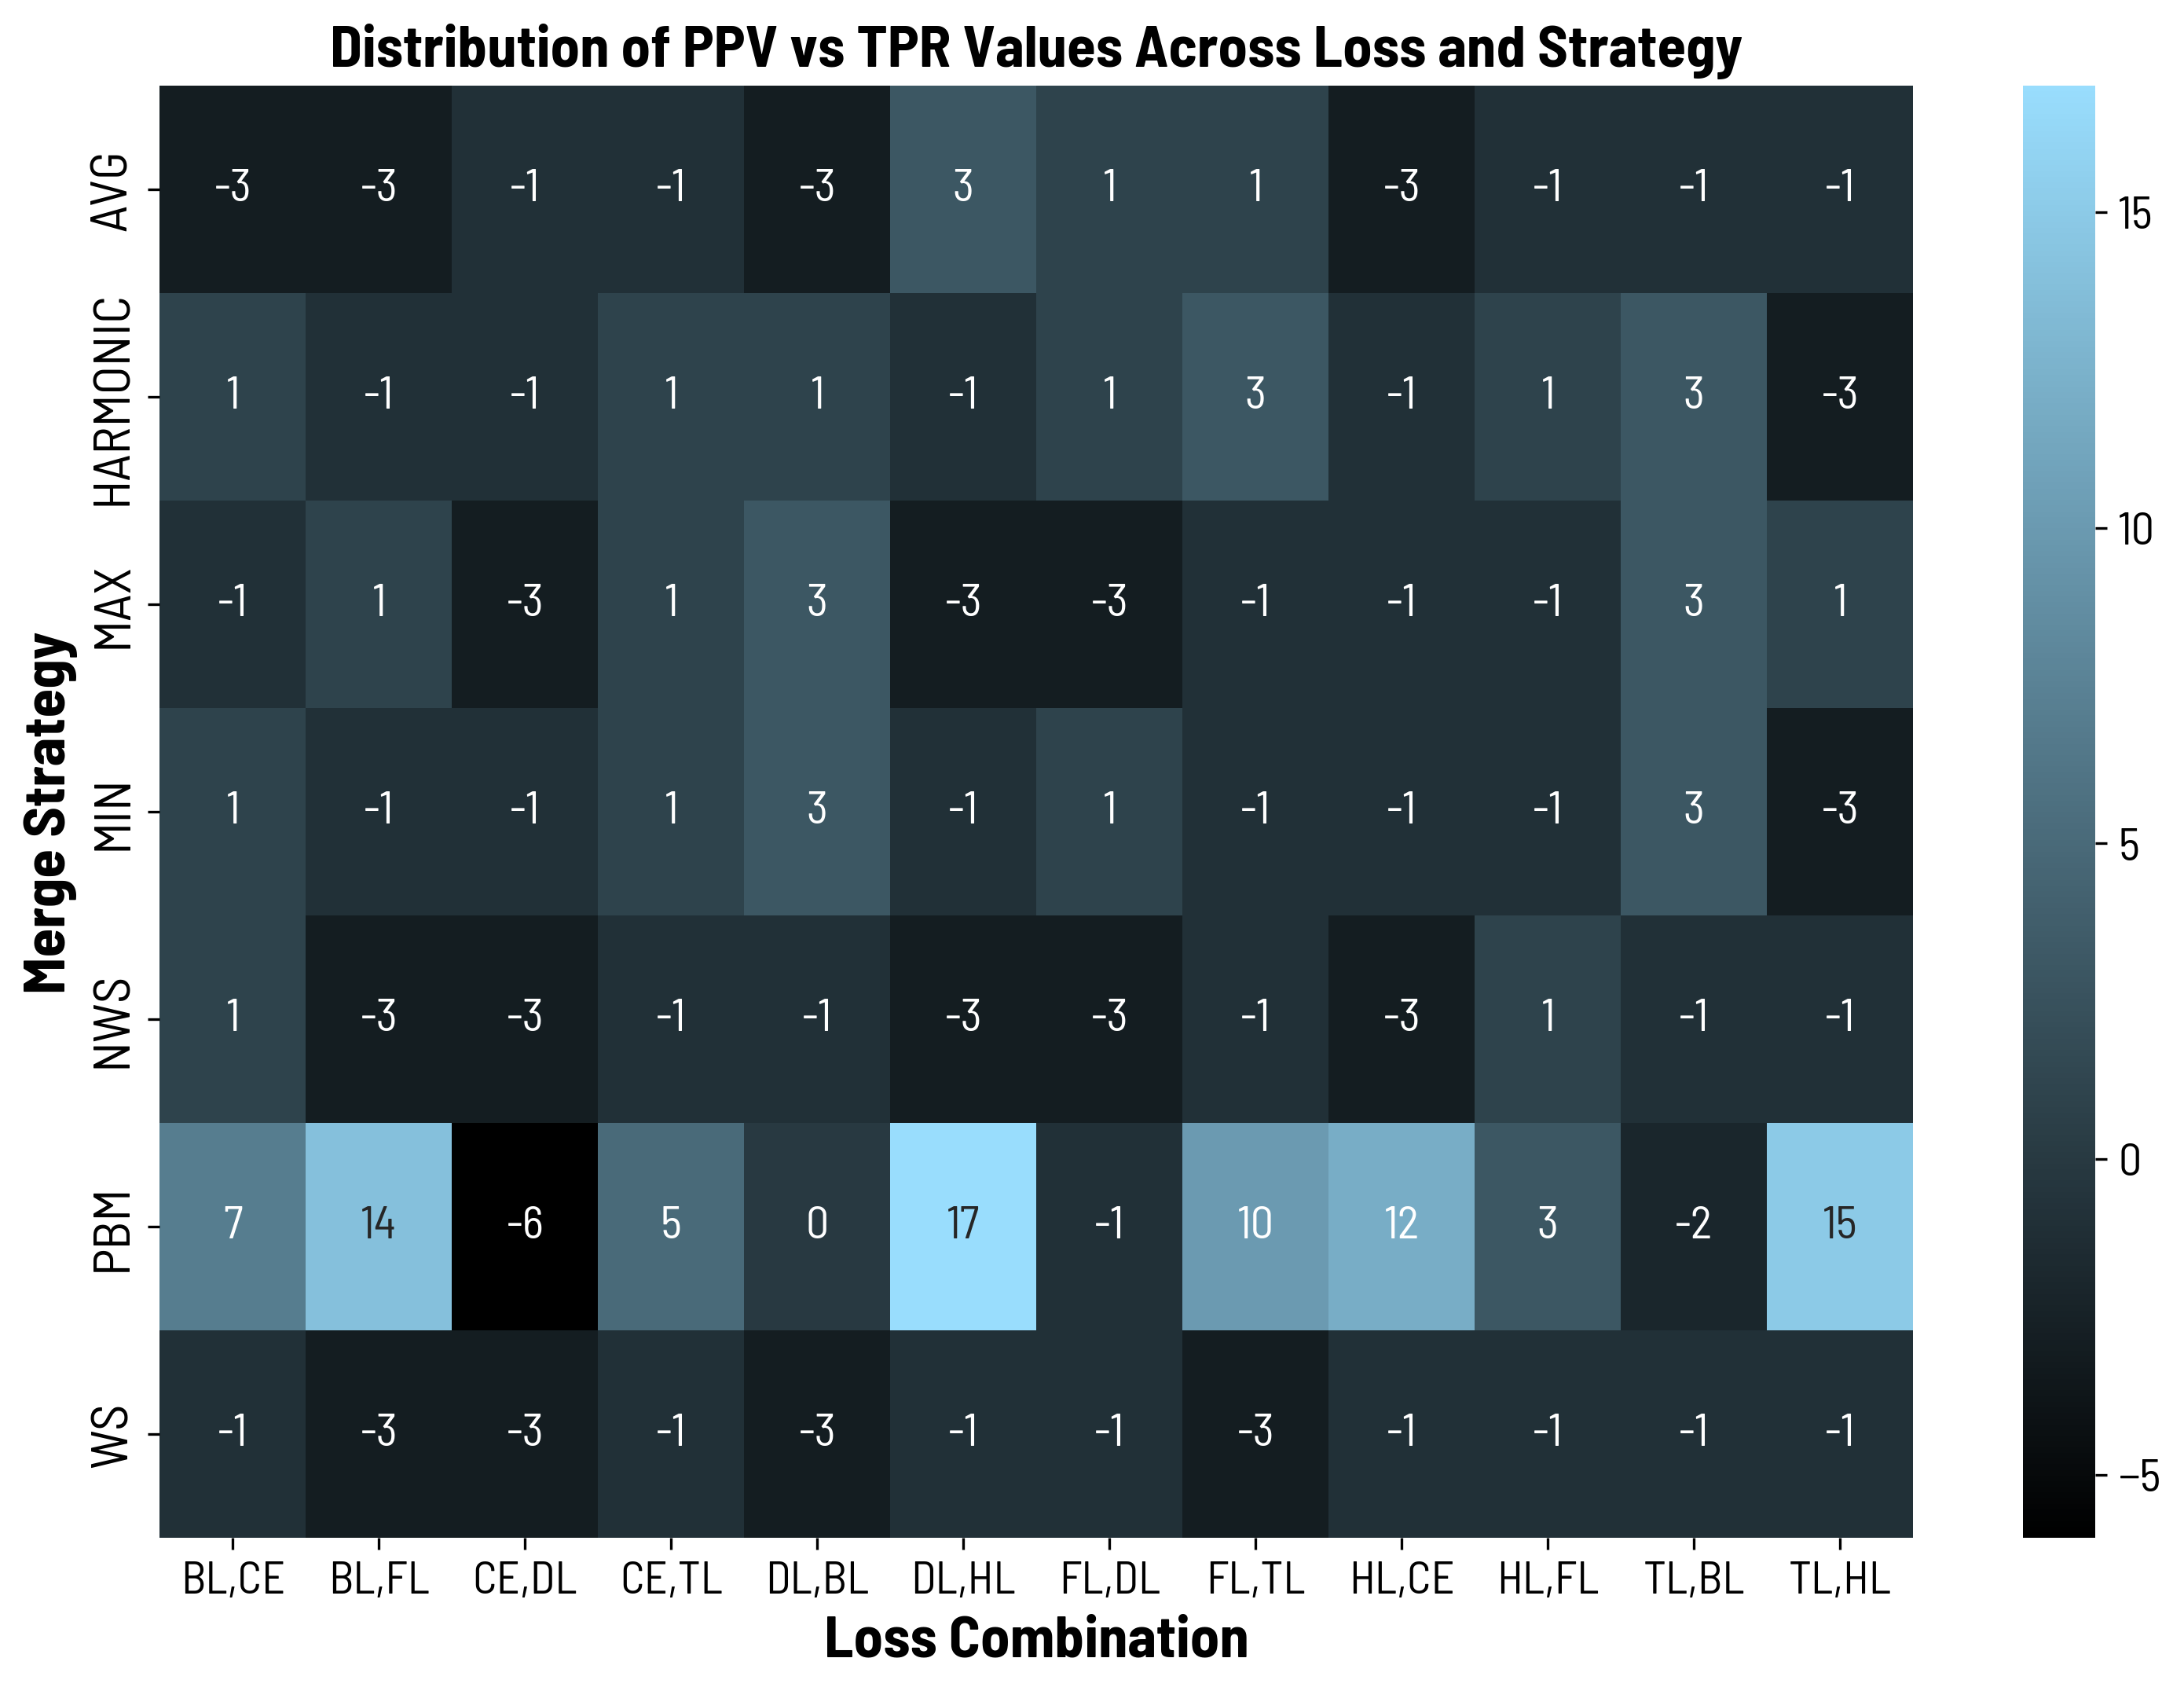
\includegraphics[width=\imgWidthcustom]{images/ppv_tpr_heatmap_double_medaka.png}}
    \subfigure[Distribution of PPV vs. TPR for triple losses]{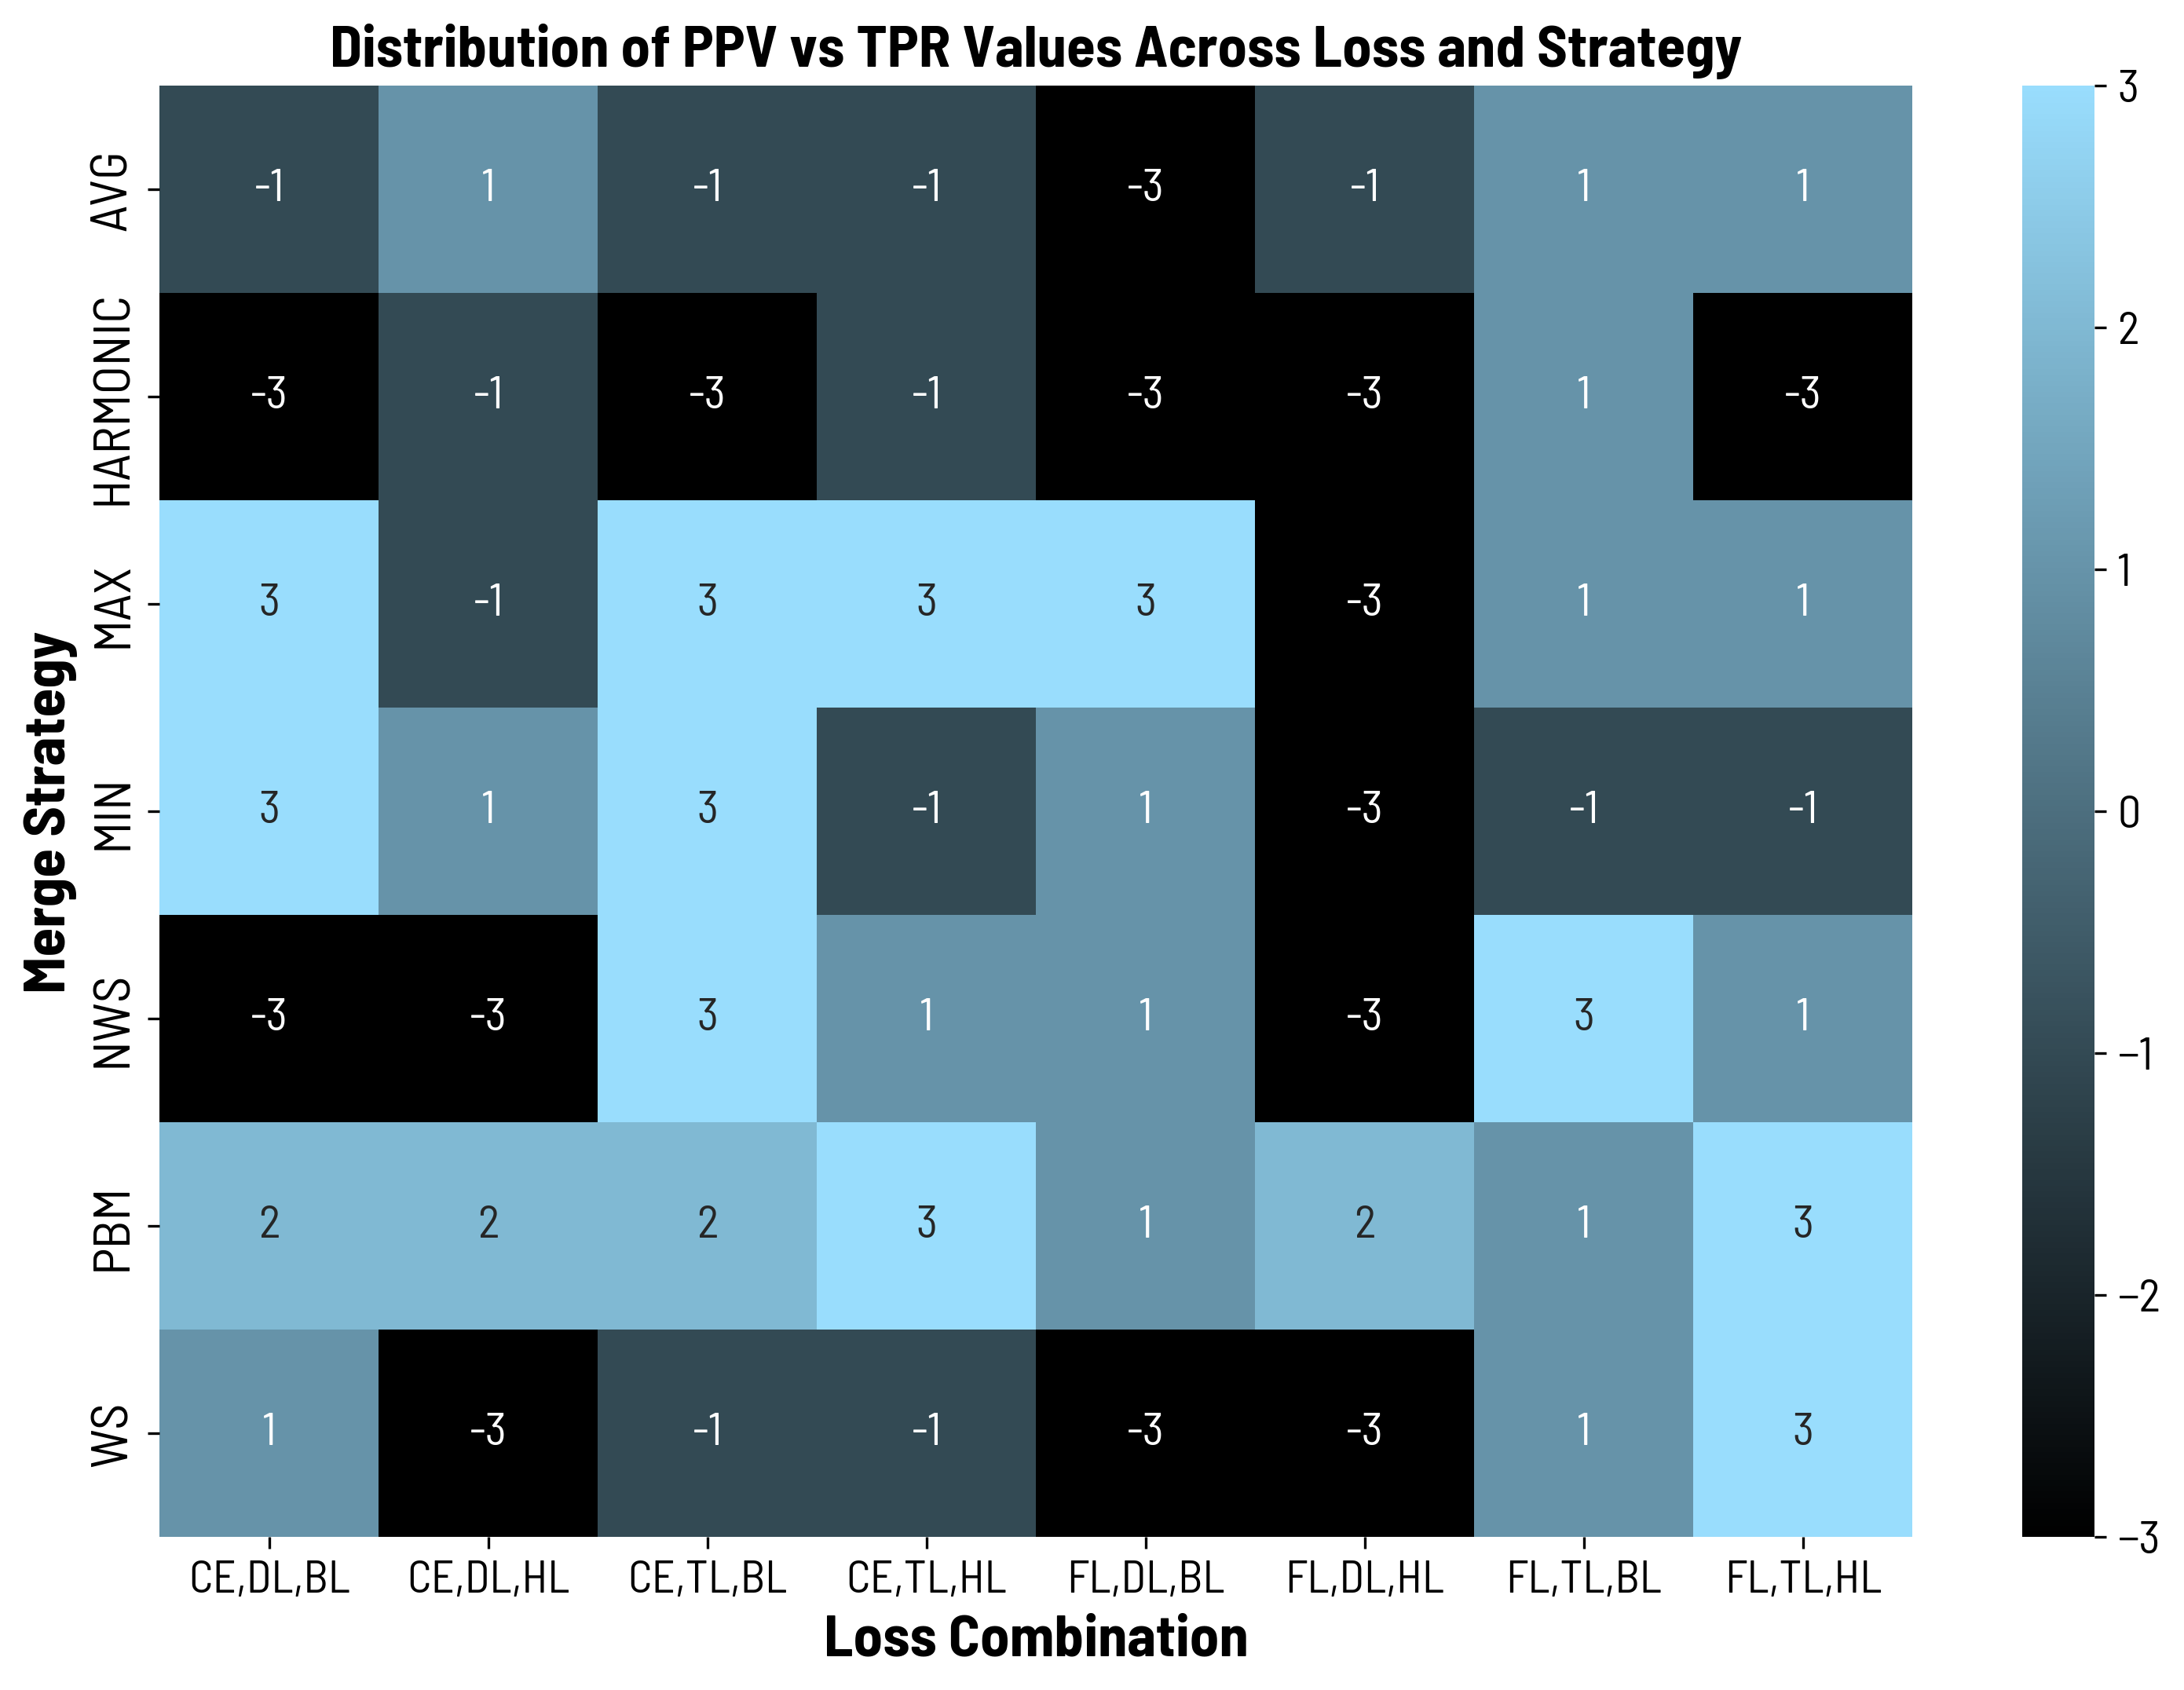
\includegraphics[width=\imgWidthcustom]{images/ppv_tpr_heatmap_triple_medaka.png}}
    \caption[Distribution of PPV vs. TPR Values]{Heatmaps visualizing the relative prevalence as a difference map of PPV and TPR across various loss combinations and merge strategies. Each cell represents a unique combination. Positive values indicate a predominance of TPR, while negative values signify a predominance of PPV.}
    \label{ppv_vs_tpr_medaka}
\end{figure}
\newpage

\subsection{Ablation study}
\begin{figure}[H]%[htbp]
    \centering
    \subfigure[Double Loss Combination for 100 \% Data Utilization]{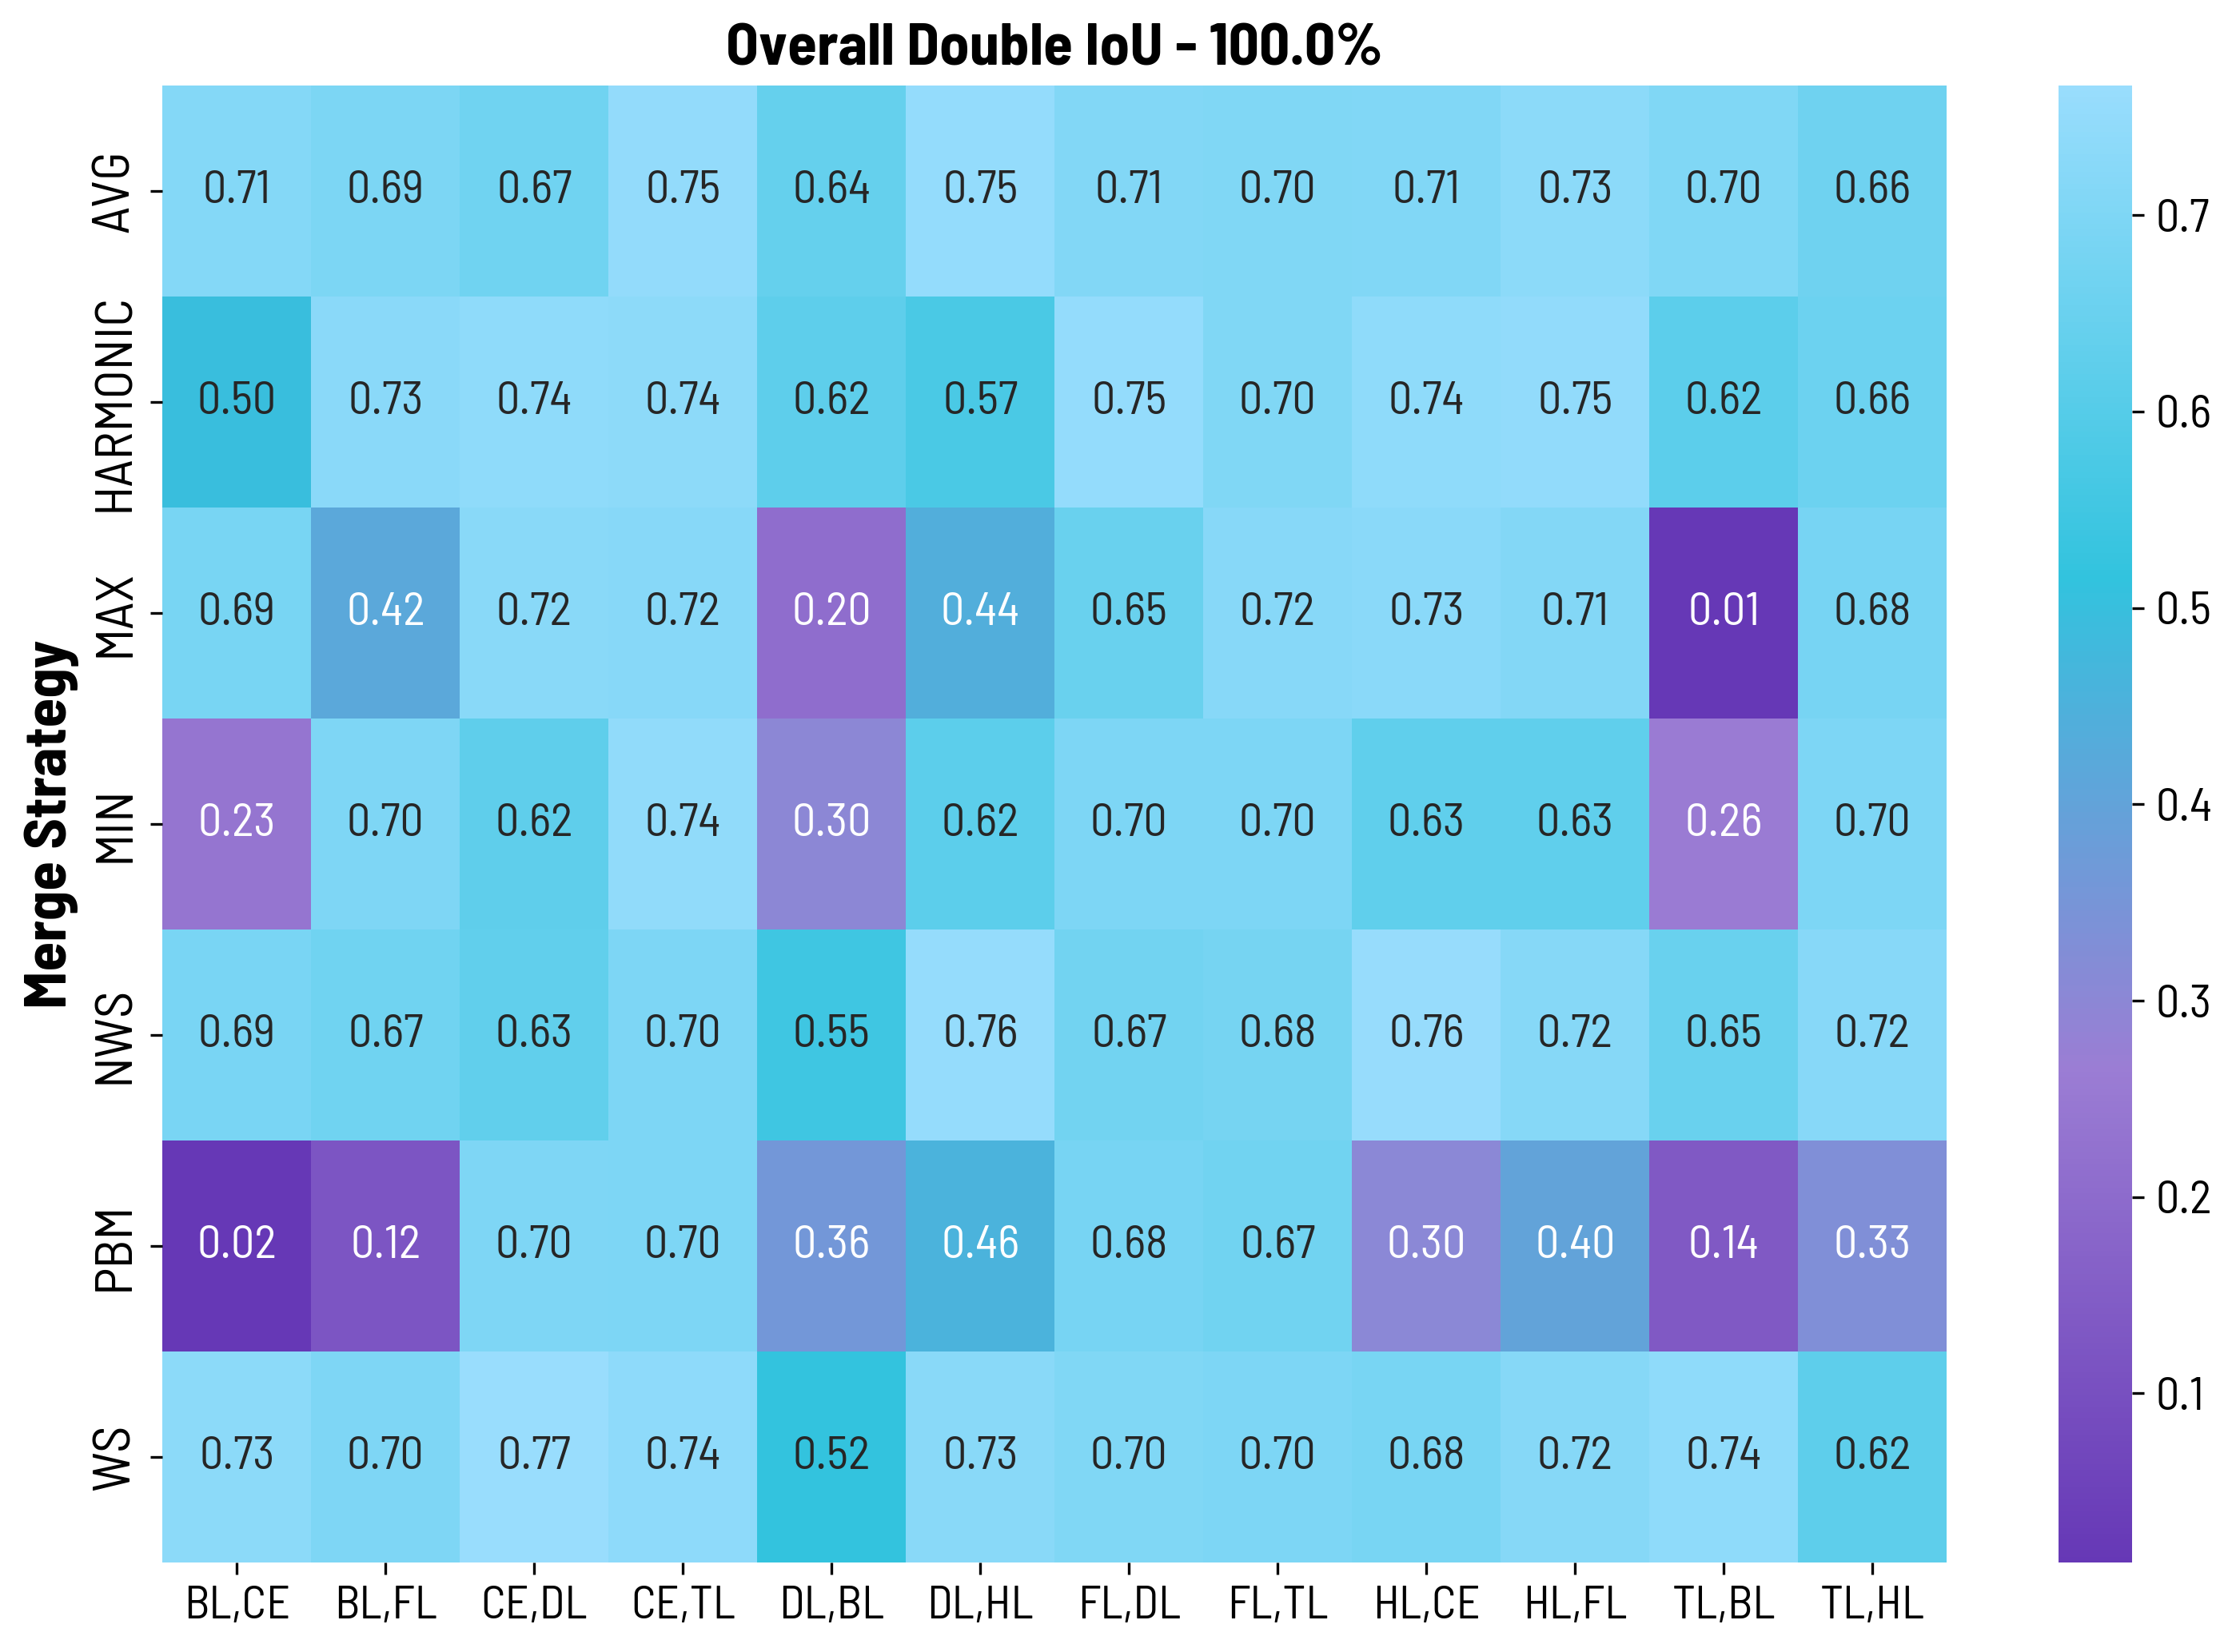
\includegraphics[width=\imgWidthcustom]{images/(1.0, 2)_ablation_summary_medaka.png}}
    \subfigure[Triple Loss Combination for 100 \% Data Utilization]{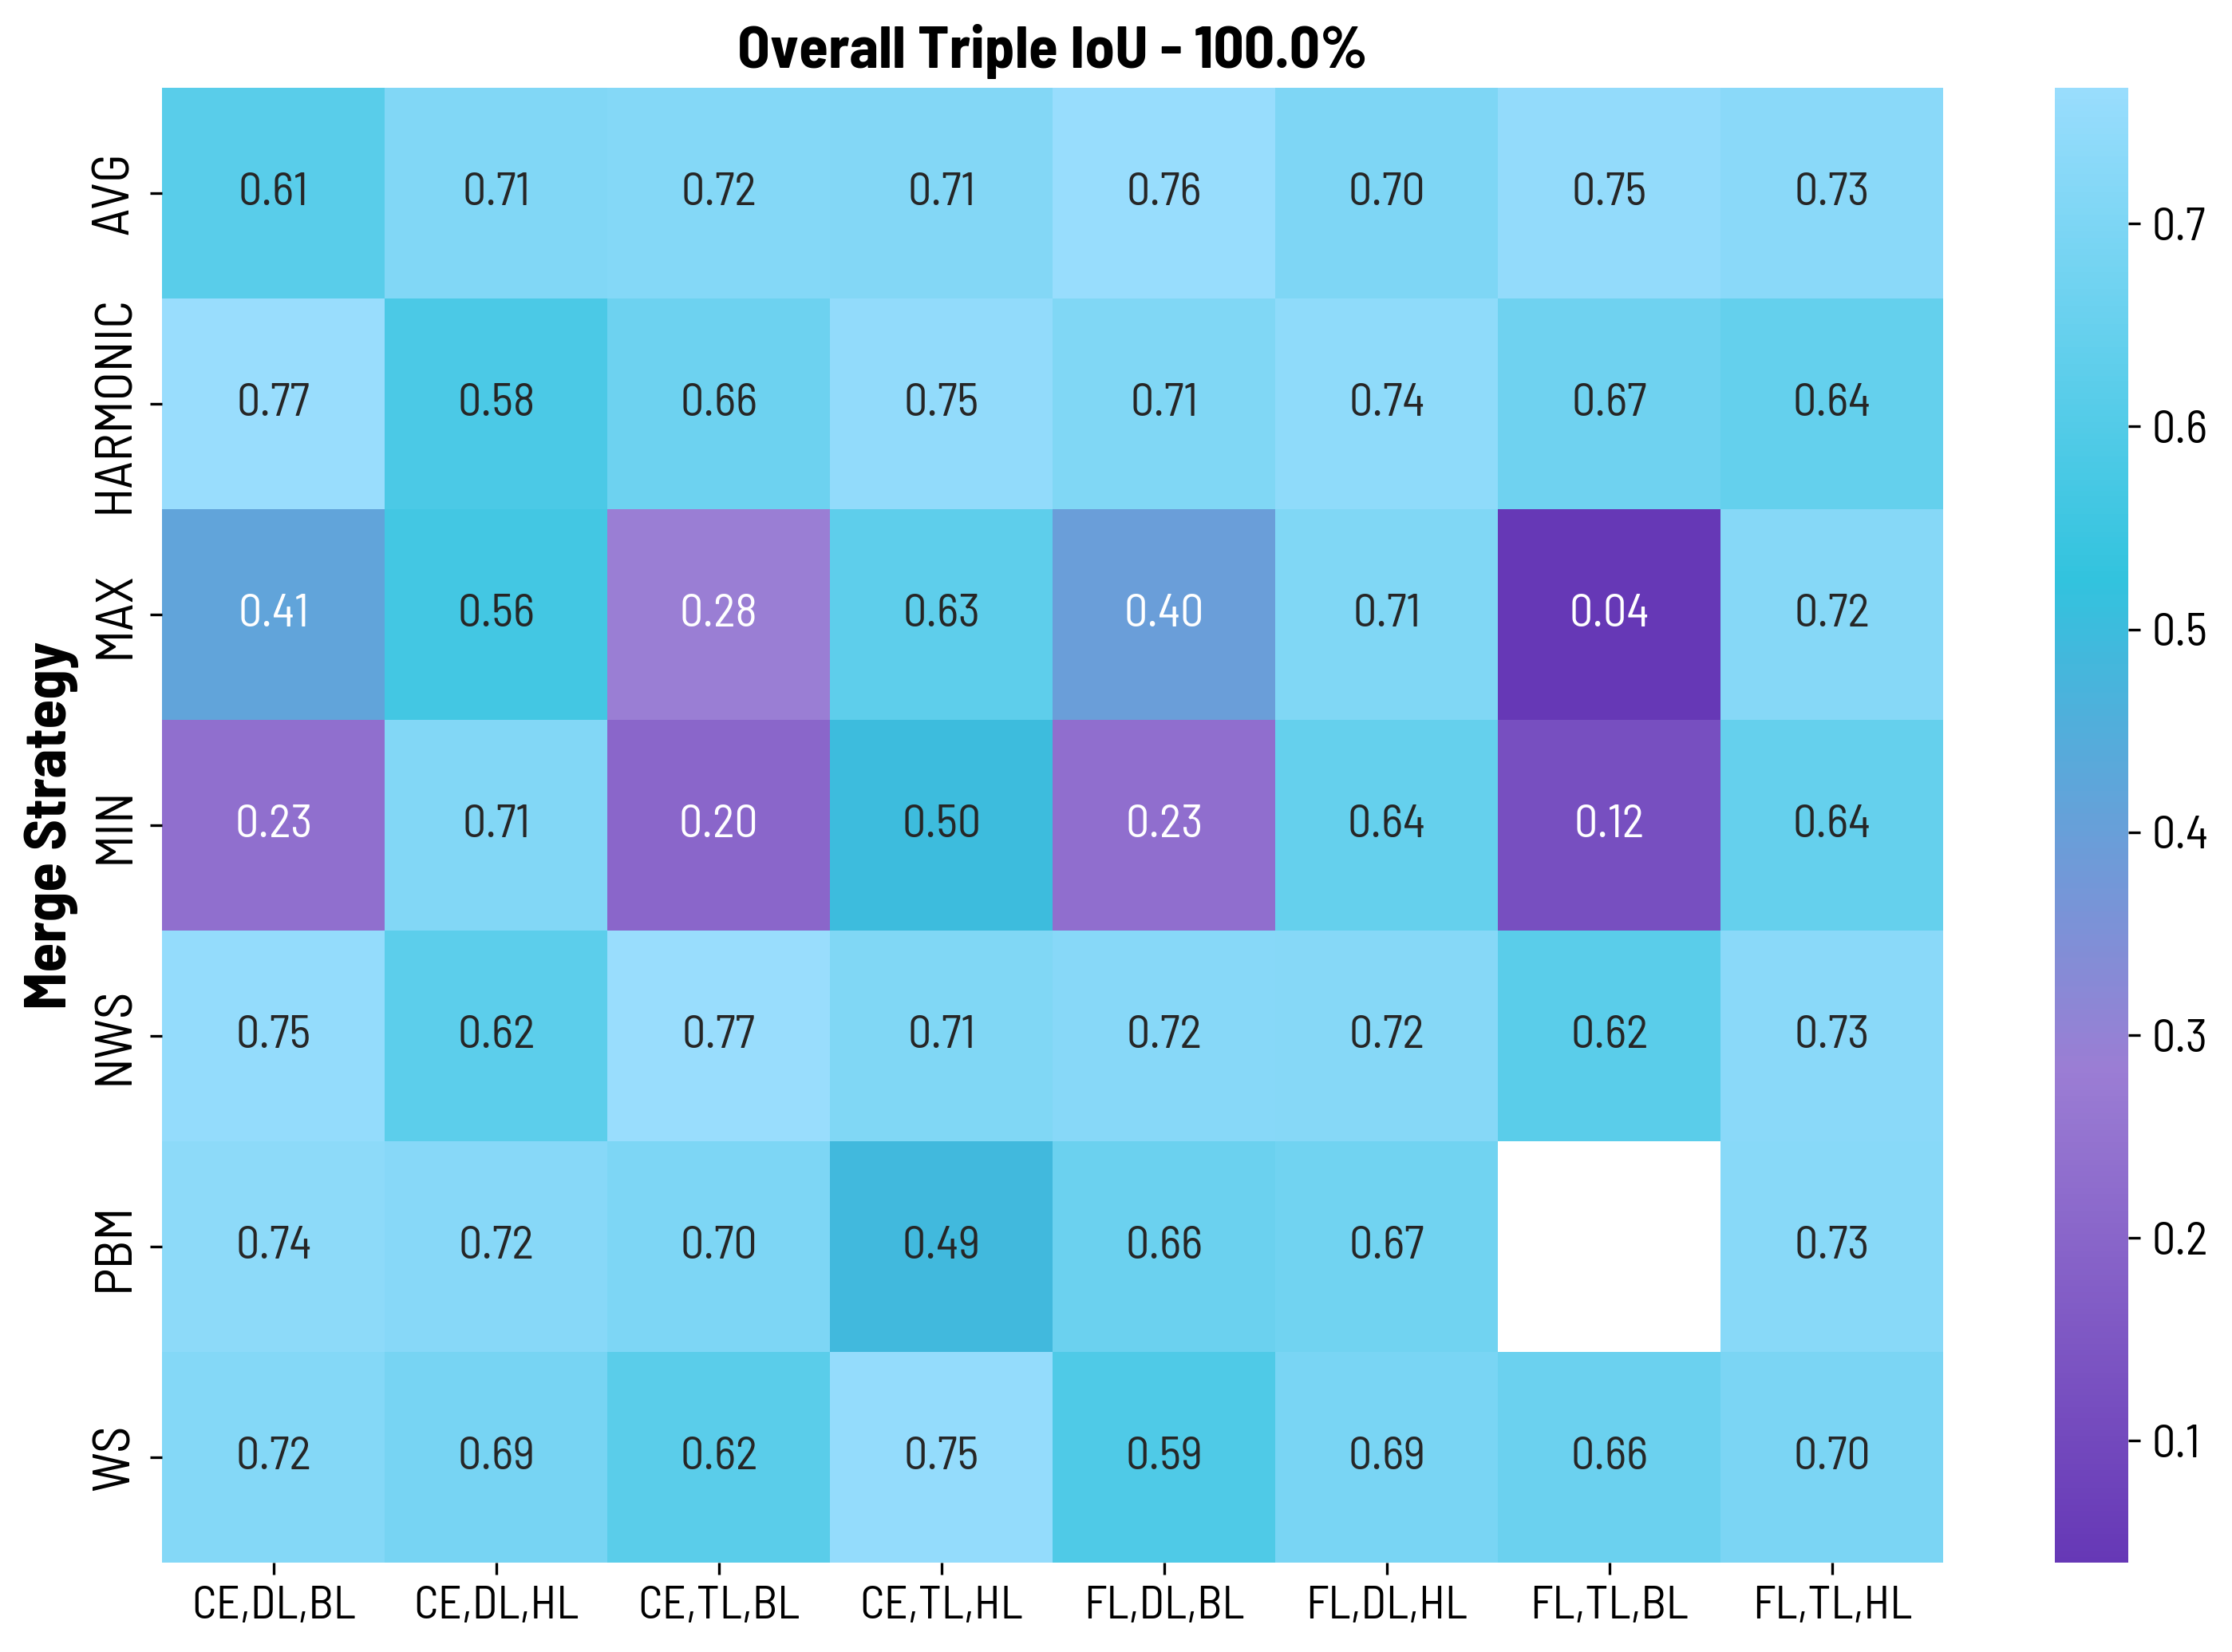
\includegraphics[width=\imgWidthcustom]{images/(1.0, 3)_ablation_summary_medaka.png}}
    \subfigure[Double Loss Combination for 64 \% Data Utilization]{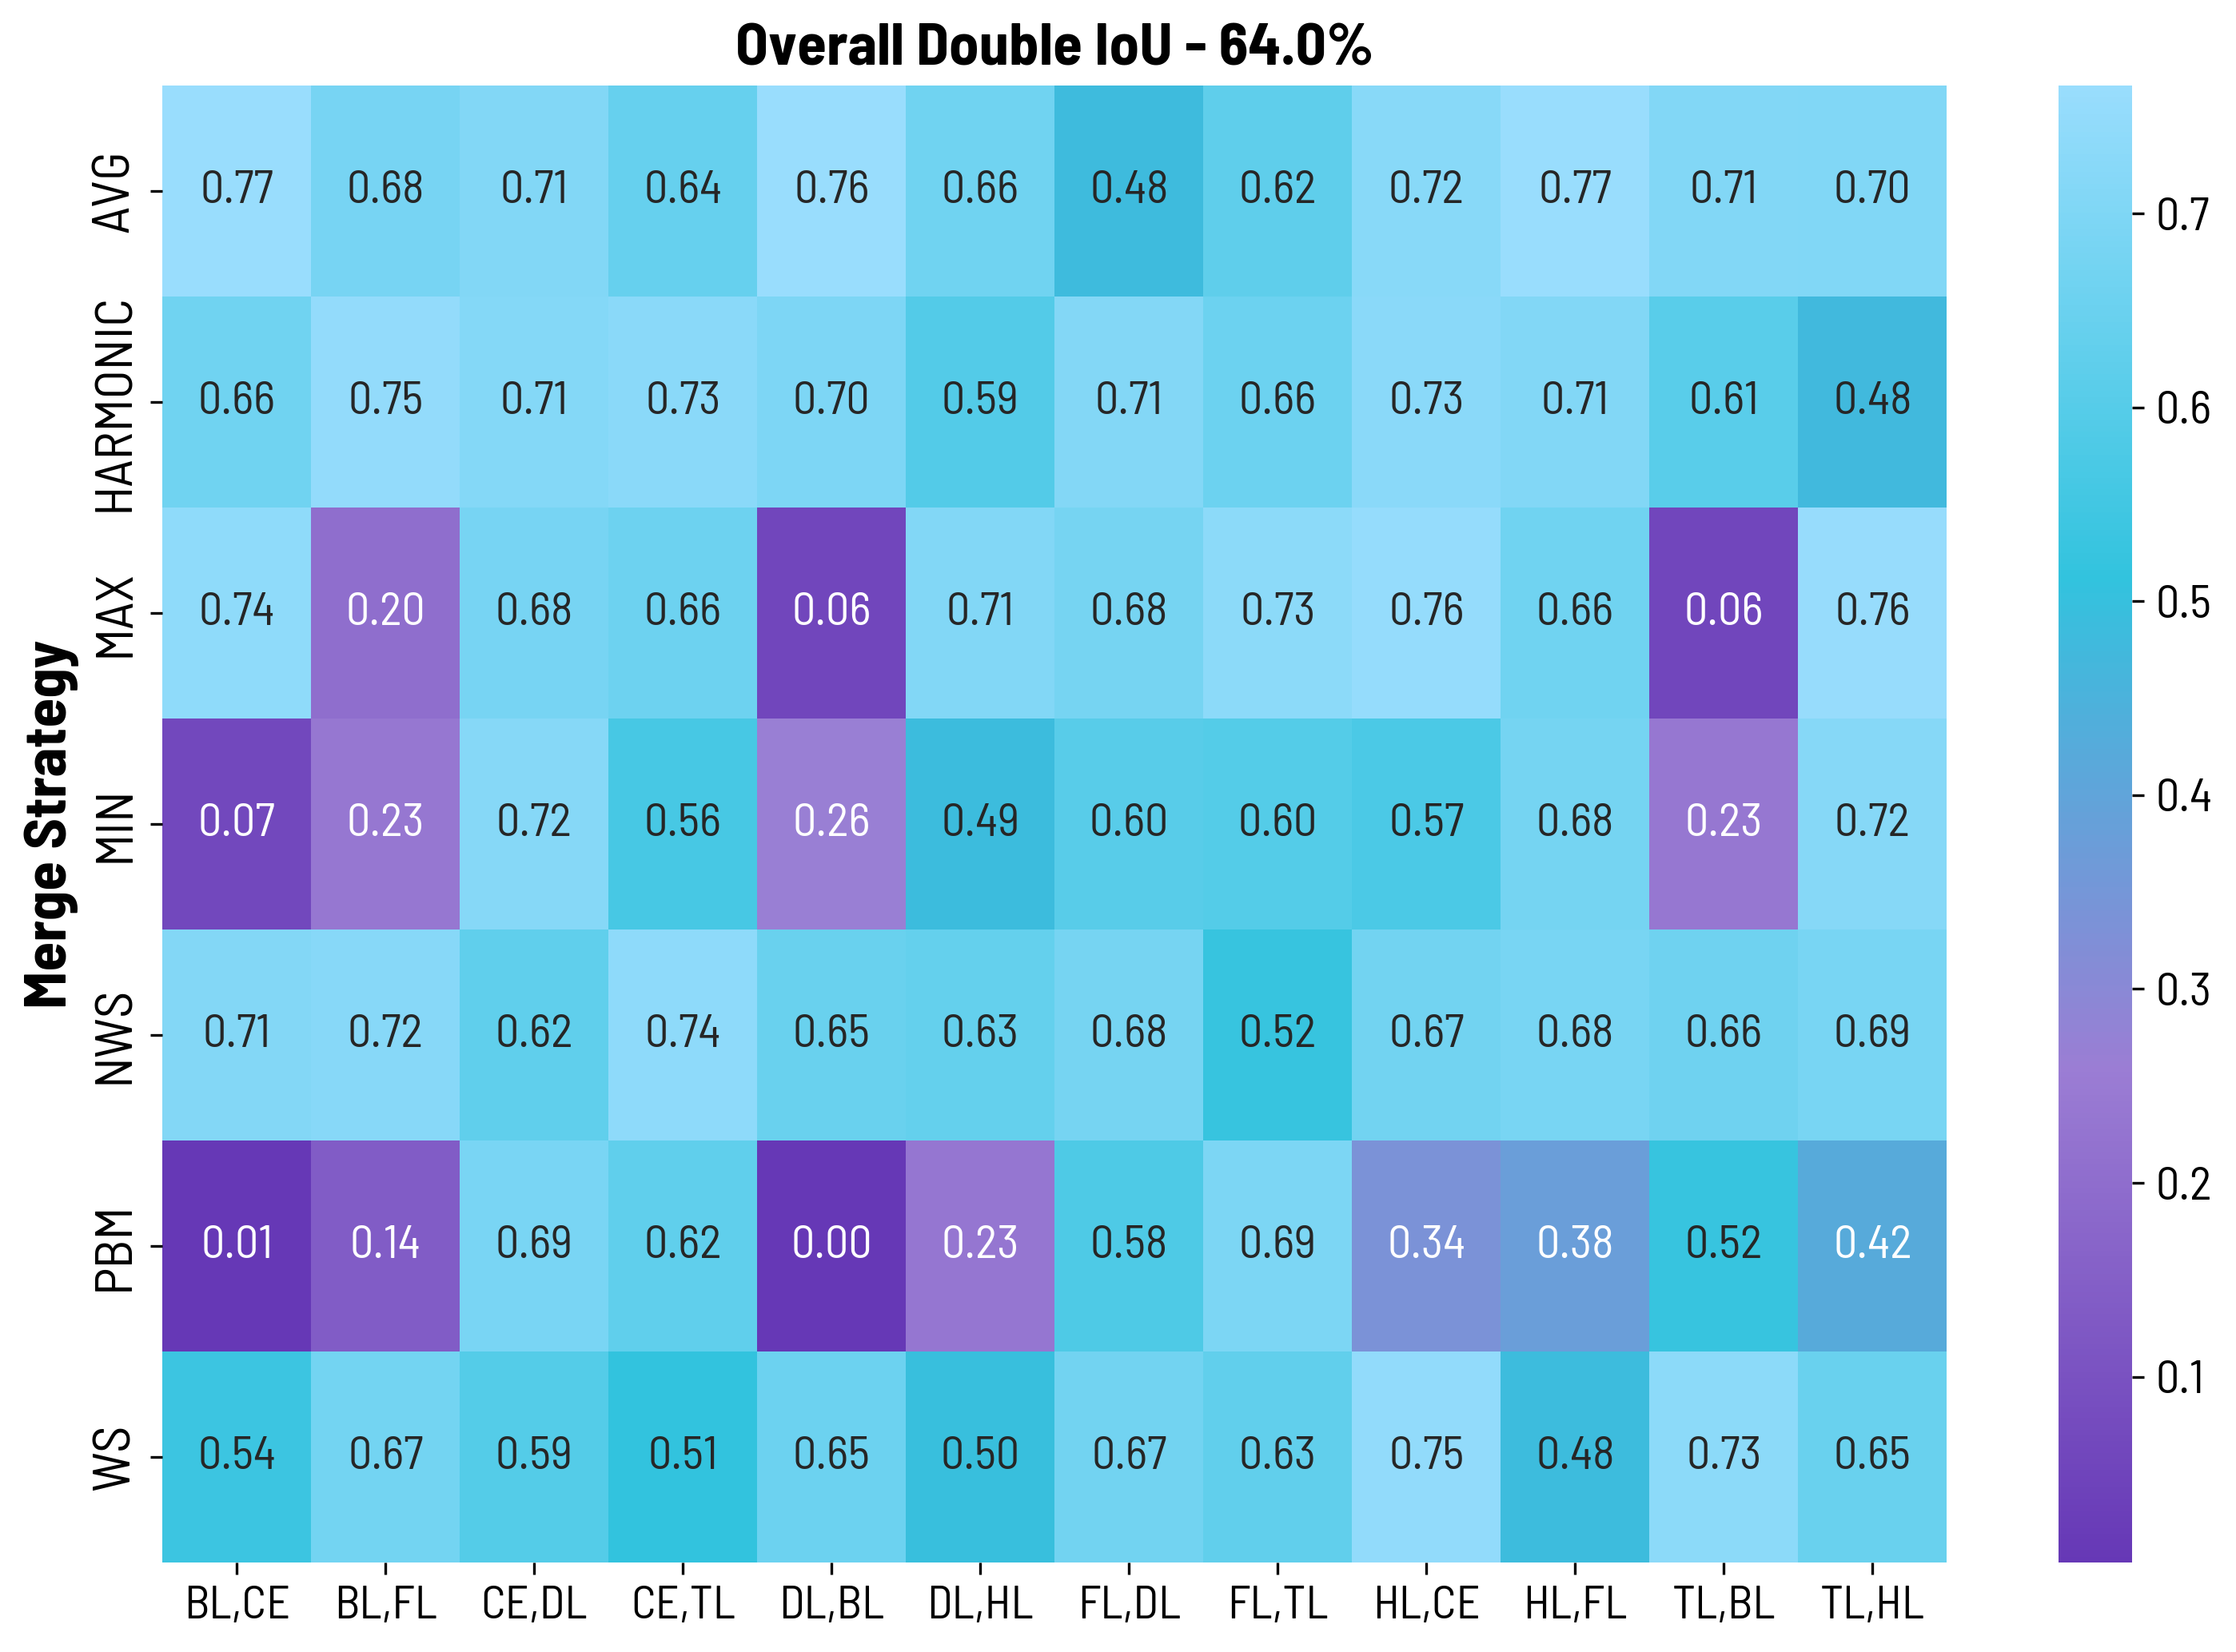
\includegraphics[width=\imgWidthcustom]{images/(0.64, 2)_ablation_summary_medaka.png}}
    \subfigure[Triple Loss Combination for 64 \% Data Utilization]{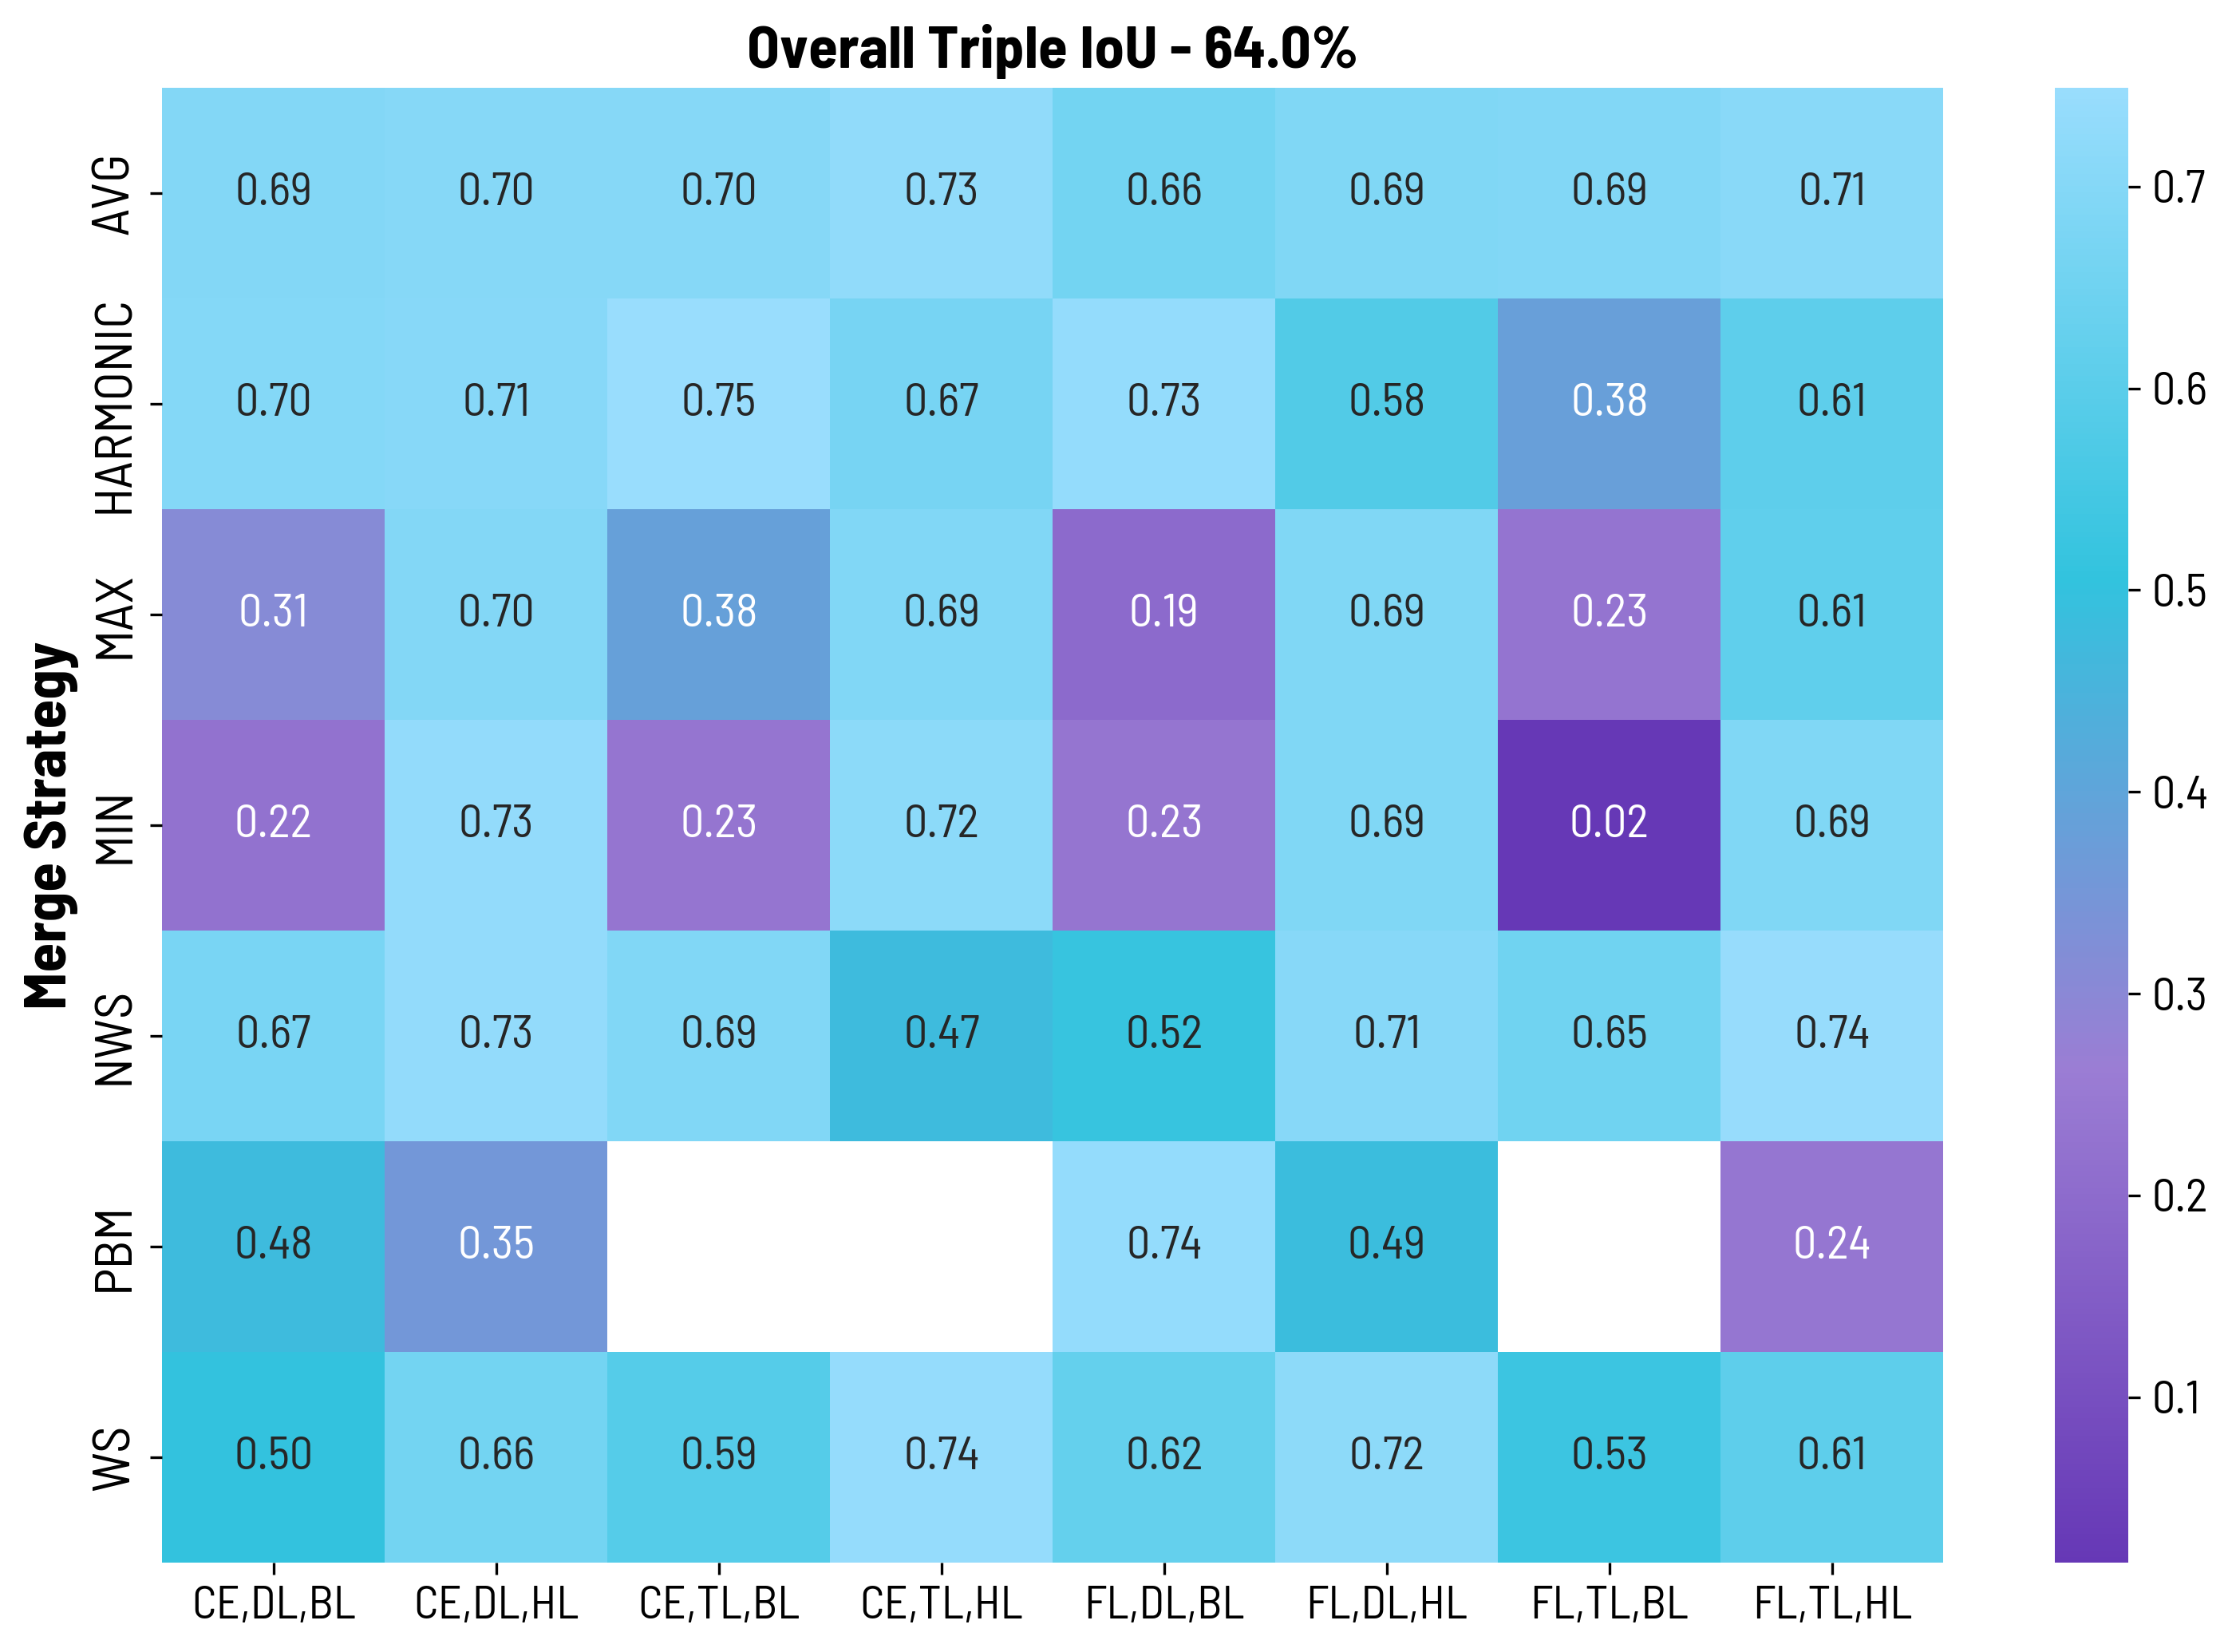
\includegraphics[width=\imgWidthcustom]{images/(0.64, 3)_ablation_summary_medaka.png}}
    \subfigure[Double Loss Combination for 32 \% Data Utilization]{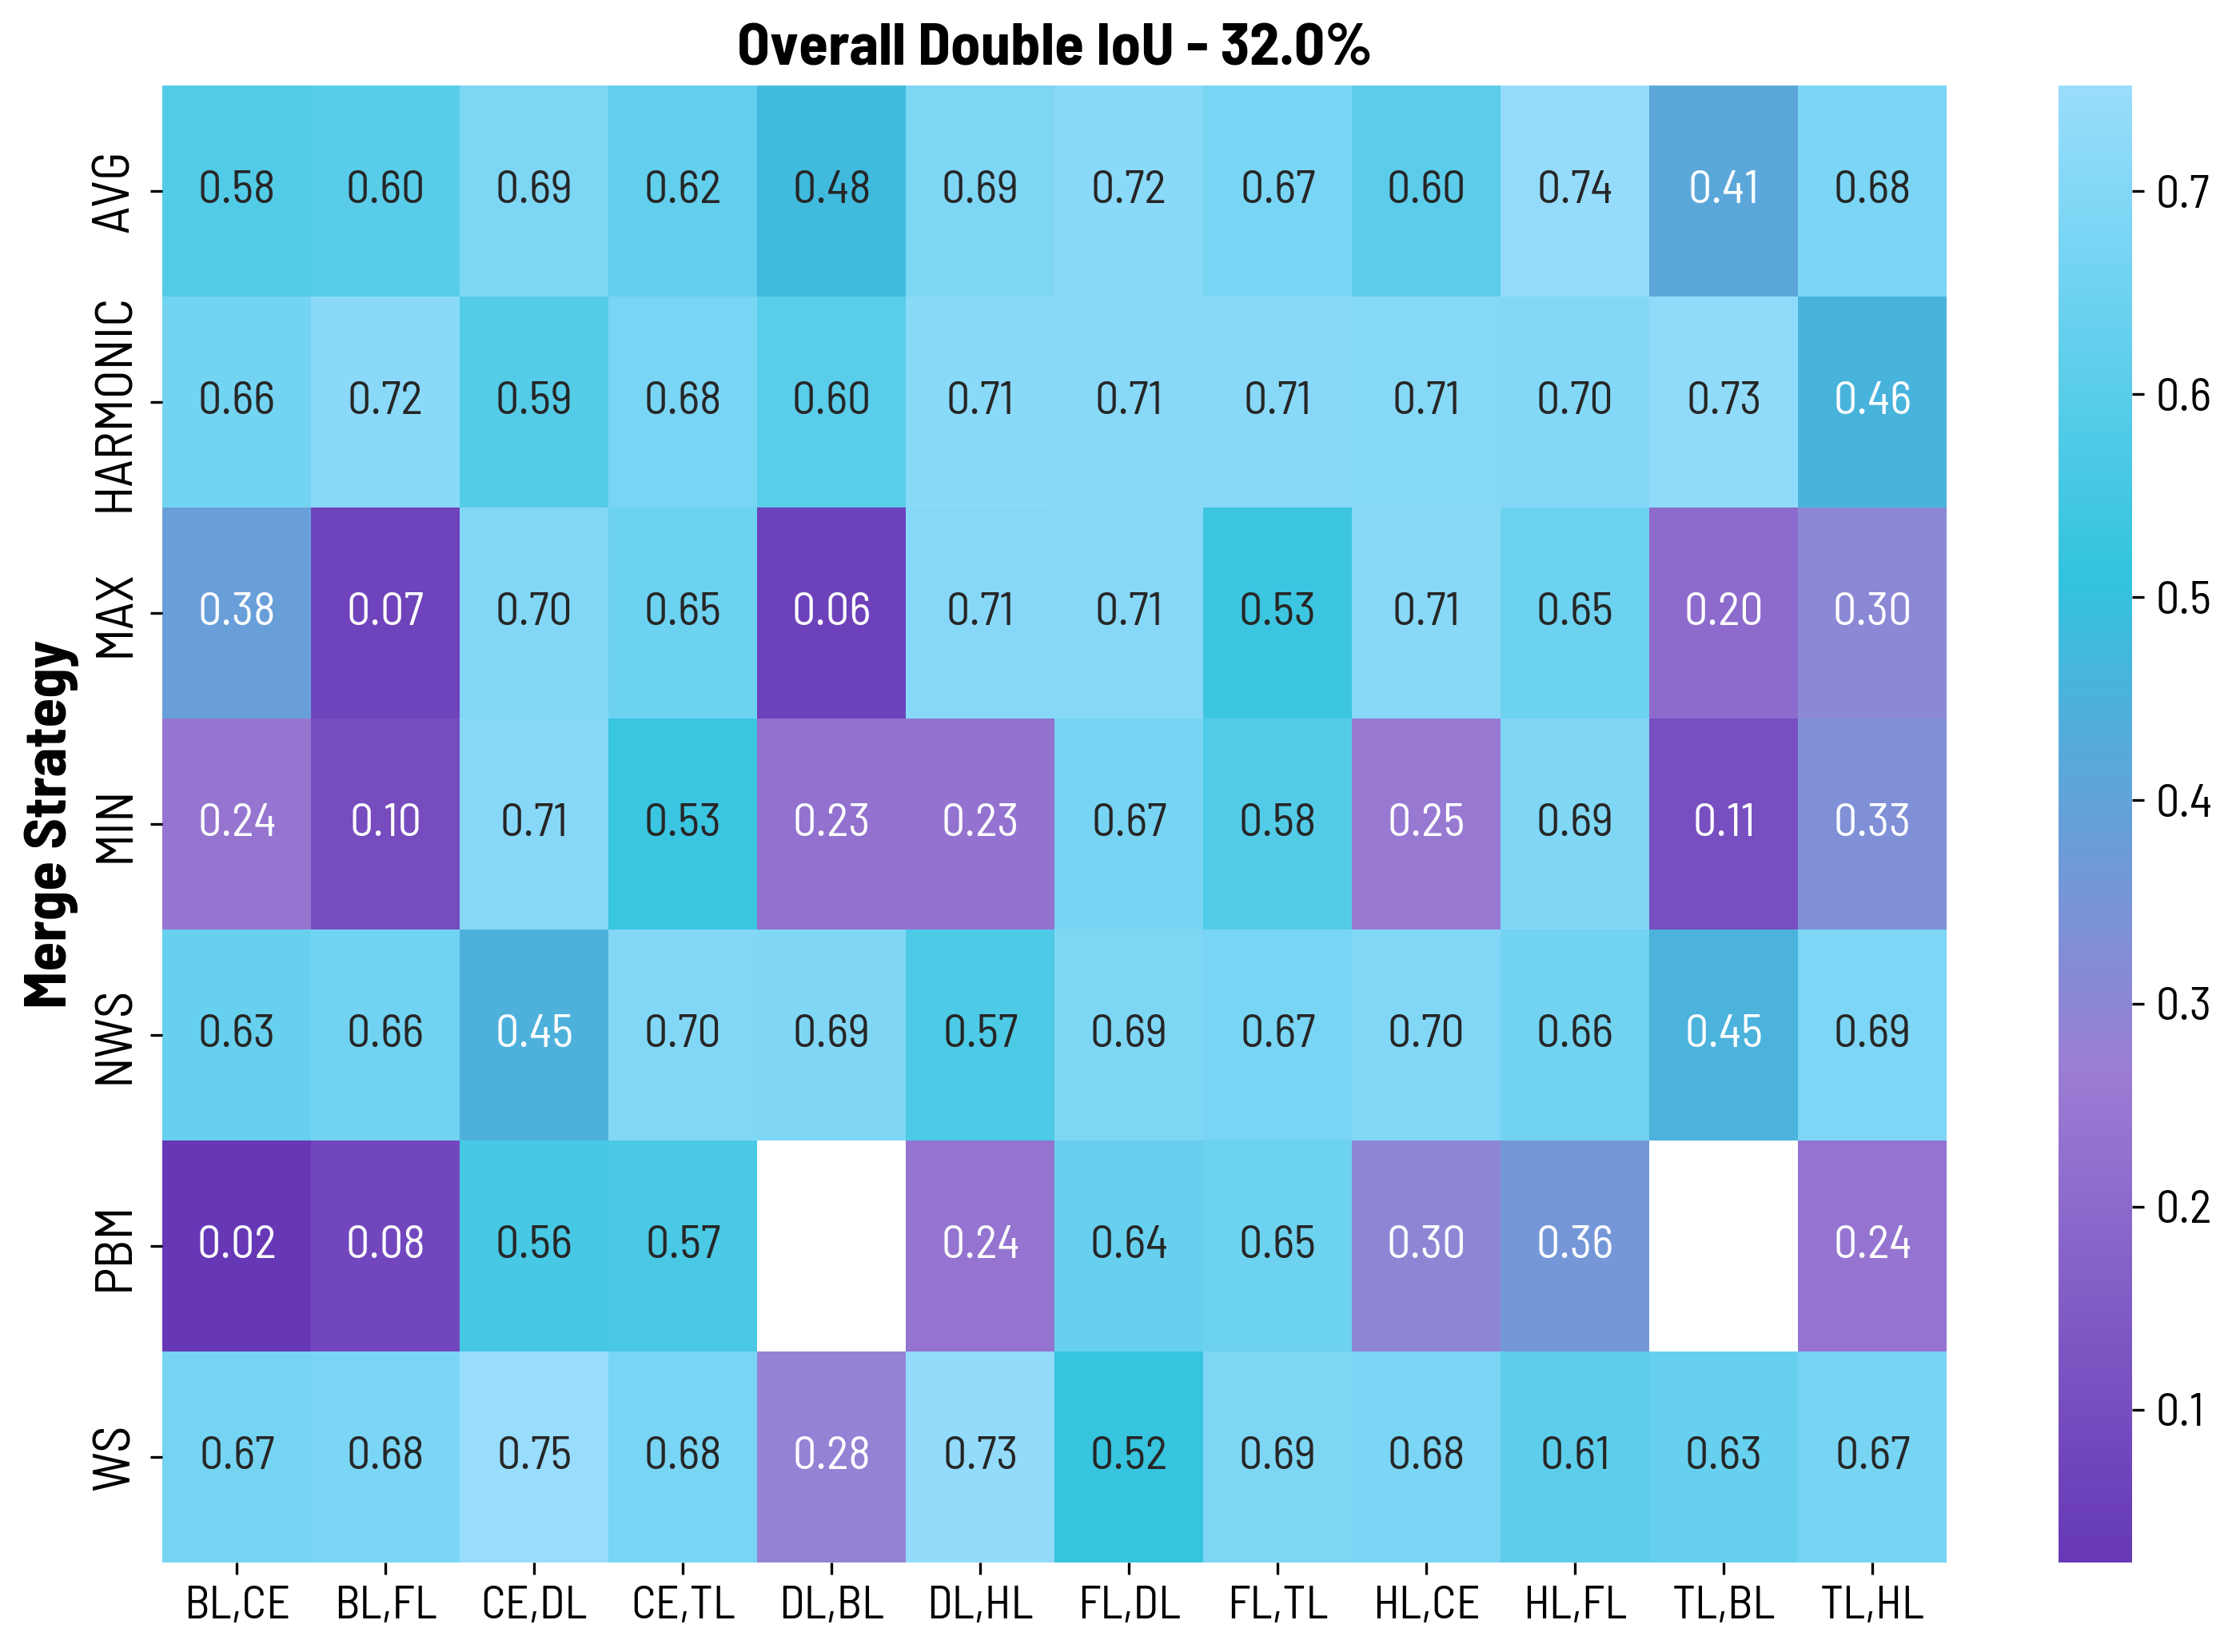
\includegraphics[width=\imgWidthcustom]{images/(0.32, 2)_ablation_summary_medaka.png}}
    \subfigure[Triple Loss Combination for 32 \% Data Utilization]{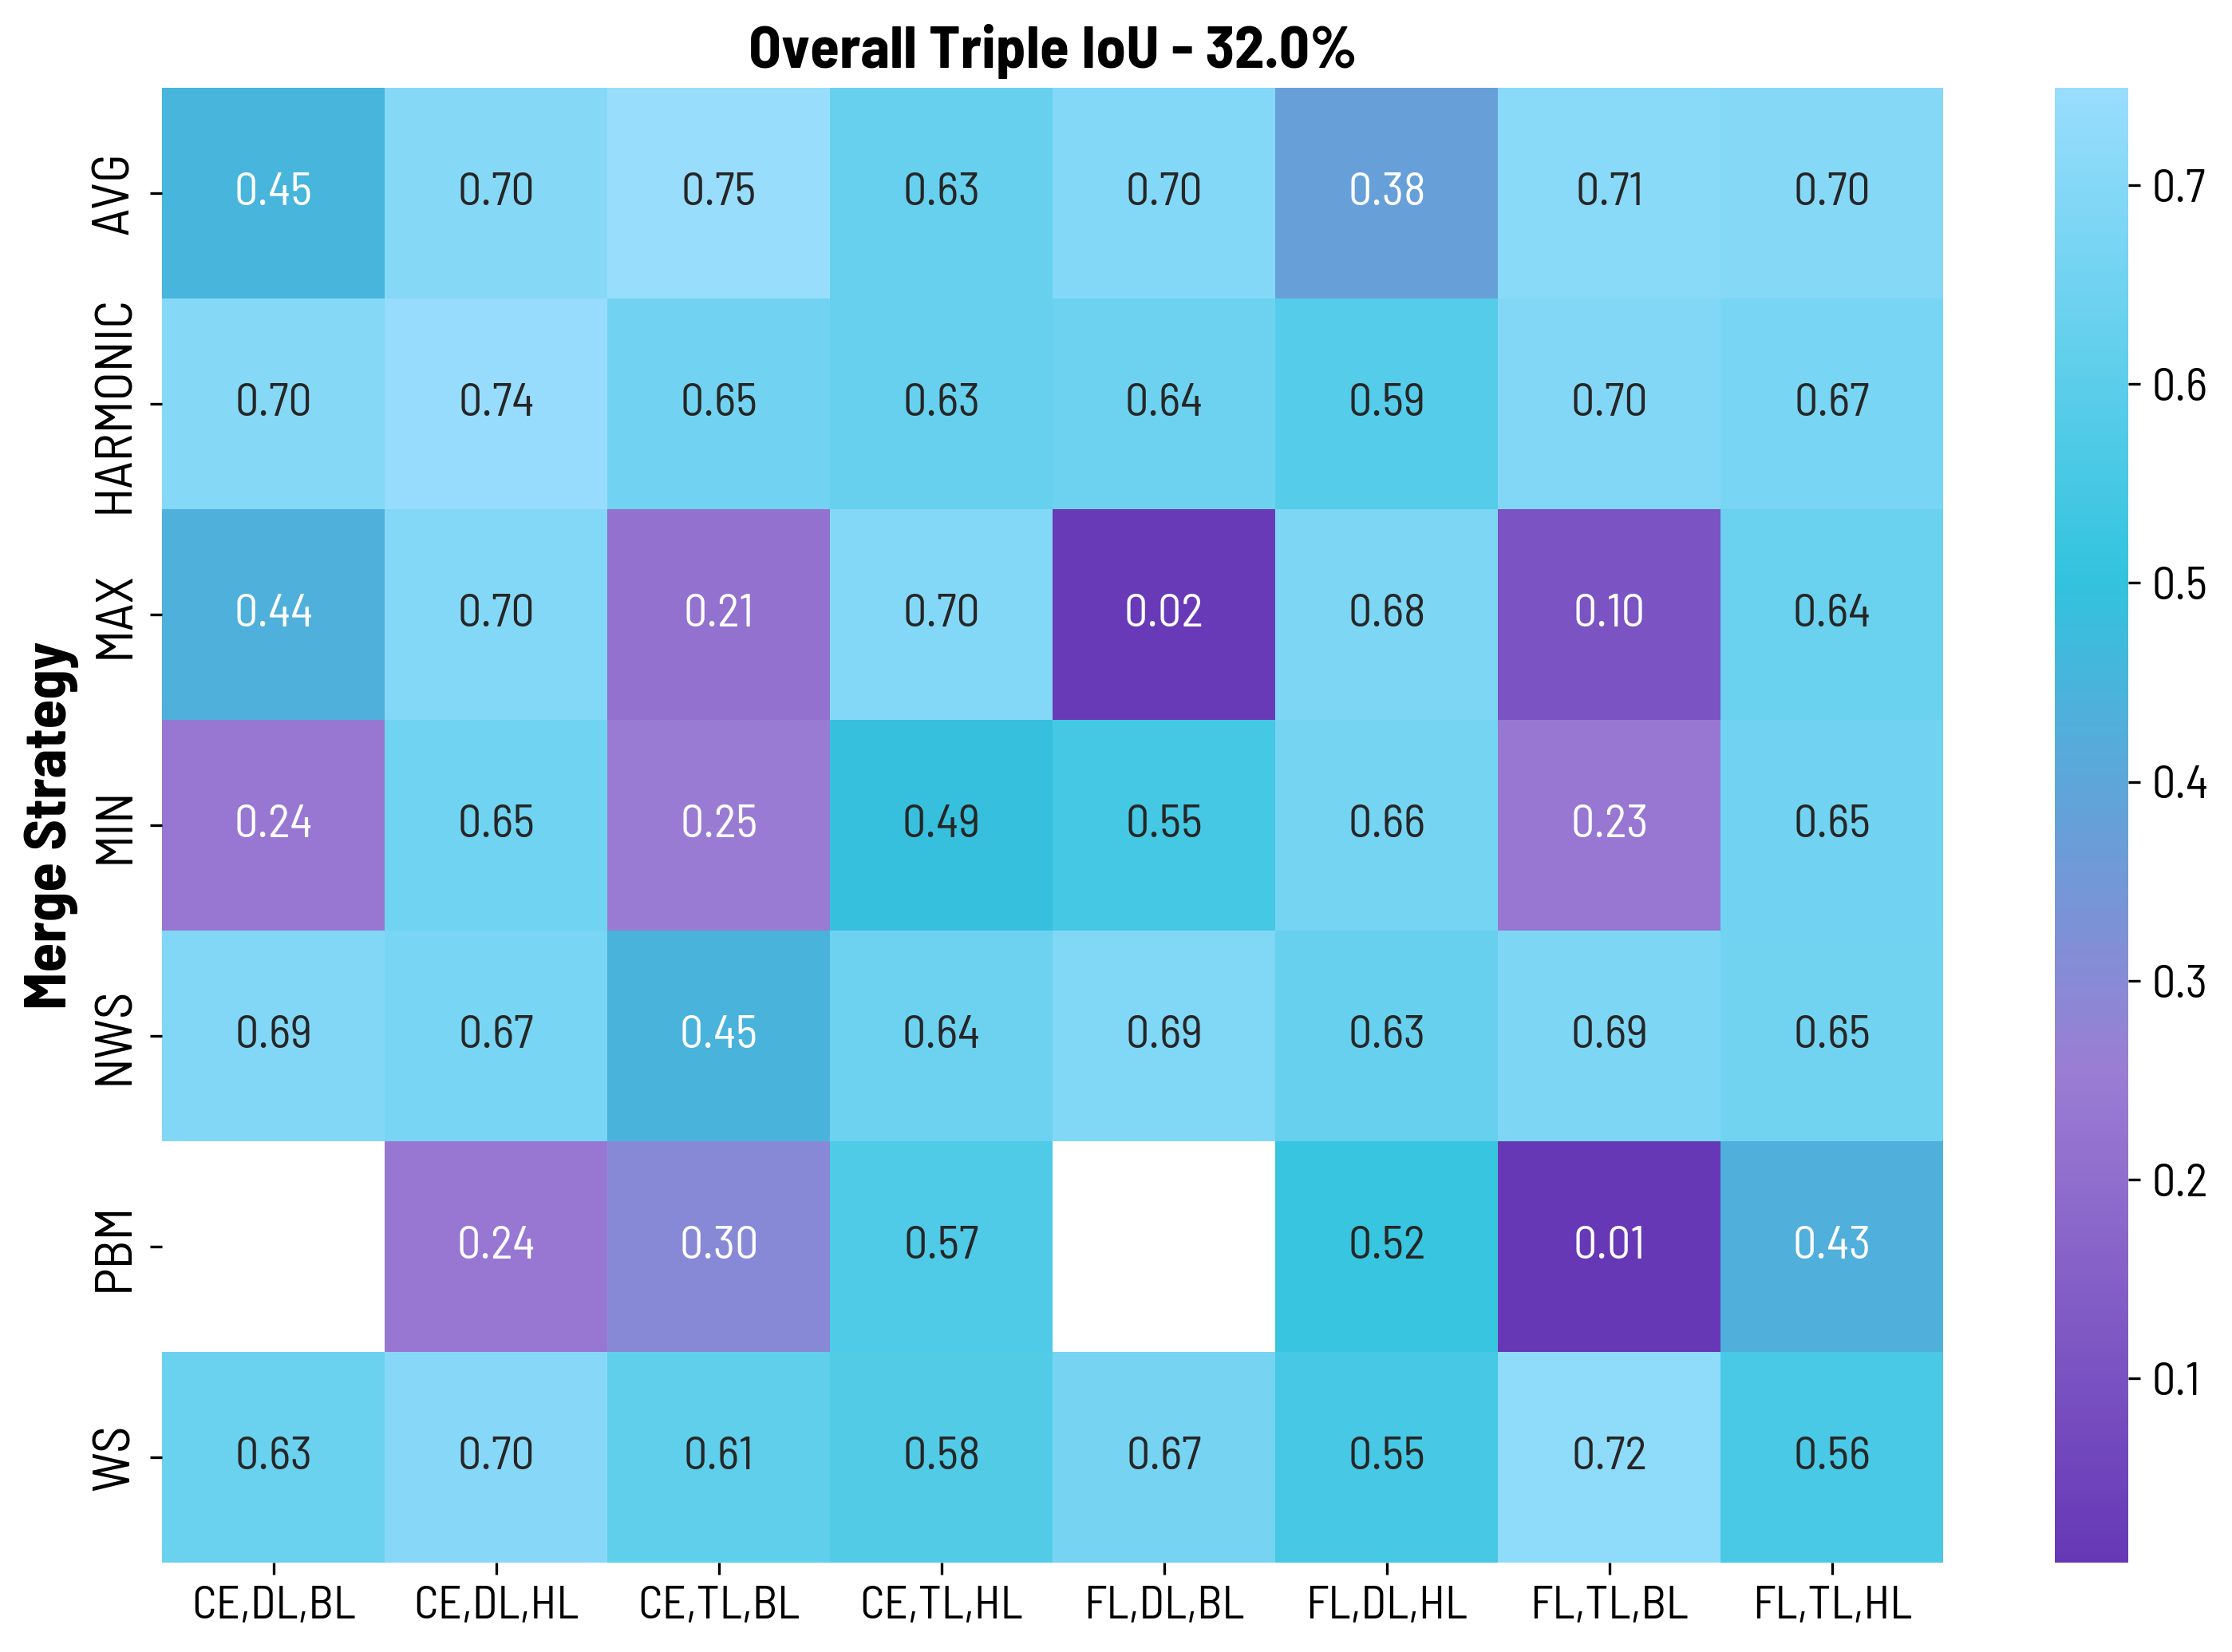
\includegraphics[width=\imgWidthcustom]{images/(0.32, 3)_ablation_summary_medaka.png}}
    \caption[Overall results for different dataset sizes]{Overall results generated from different dataset sizes. The left column (a,c,e) illustrates results from double loss combinations, while the right column (b,d,f) depicts results from triple loss combinations.}
    \label{ablation_medaka_heatmaps}
\end{figure}
\newpage

%----------------------------------------------------------------------------------------%
%---------------------------------------Skin lesion--------------------------------------%
%----------------------------------------------------------------------------------------%
\section{Skin lesion}
\label{sec:supplementary_skin_lesion}
\subsection{Baseline}
\label{subsec:baseline_skin_lesion}
% Please add the following required packages to your document preamble:
% \usepackage{graphicx}
% \usepackage[table,xcdraw]{xcolor}
% If you use beamer only pass "xcolor=table" option, i.e. \documentclass[xcolor=table]{beamer}
\begin{table}[H]
  \centering
  \resizebox{\textwidth}{!} &
    {\color[HTML]{FFFFFF} Iou} &
    {\color[HTML]{FFFFFF} PPV} &
    {\color[HTML]{FFFFFF} TPR} &
    {\color[HTML]{FFFFFF} PPV vs. TPR} \\ \hline
  \multicolumn{1}{|c|}{1} &
    \multicolumn{1}{c|}{55} &
    \cellcolor[HTML]{6638B6}{\color[HTML]{FFFFFF} DB} &
    \textit{CE} &
    0.64 &
    \textit{0.667} &
    \textit{0.812} &
    \textit{0.824} &
    TPR \\ \hline
  \multicolumn{1}{|c|}{2} &
    \multicolumn{1}{c|}{29} &
    \cellcolor[HTML]{6638B6}{\color[HTML]{FFFFFF} DB} &
    \textit{CE} &
    0.32 &
    \textit{0.640} &
    \textit{0.780} &
    \textit{0.819} &
    TPR \\ \hline
  \multicolumn{1}{|c|}{3} &
    \multicolumn{1}{c|}{29} &
    \cellcolor[HTML]{6638B6}{\color[HTML]{FFFFFF} DB} &
    \textit{CE} &
    0.32 &
    \textit{0.626} &
    \textit{0.807} &
    \textit{0.752} &
    PPV \\ \hline
  \multicolumn{1}{|c|}{4} &
    \multicolumn{1}{c|}{29} &
    \cellcolor[HTML]{6638B6}{\color[HTML]{FFFFFF} DB} &
    \textit{CE} &
    0.32 &
    \textit{0.584} &
    \textit{0.745} &
    \textit{0.699} &
    PPV \\ \hline
  \multicolumn{1}{|c|}{5} &
    \multicolumn{1}{c|}{63} &
    \cellcolor[HTML]{6638B6}{\color[HTML]{FFFFFF} DB} &
    \textit{CE} &
    0.64 &
    \textit{0.580} &
    \textit{0.752} &
    \textit{0.704} &
    PPV \\ \hline
  \multicolumn{1}{|c|}{6} &
    \multicolumn{1}{c|}{83} &
    \cellcolor[HTML]{6638B6}{\color[HTML]{FFFFFF} DB} &
    \textit{CE} &
    1.00 &
    \textit{0.532} &
    \textit{0.753} &
    \textit{0.670} &
    PPV \\ \hline
  \multicolumn{1}{|c|}{7} &
    \multicolumn{1}{c|}{97} &
    \cellcolor[HTML]{6638B6}{\color[HTML]{FFFFFF} DB} &
    \textit{CE} &
    1.00 &
    \textit{0.528} &
    \textit{0.769} &
    \textit{0.641} &
    PPV \\ \hline
  \multicolumn{1}{|c|}{8} &
    \multicolumn{1}{c|}{55} &
    \cellcolor[HTML]{6638B6}{\color[HTML]{FFFFFF} DB} &
    CE &
    0.64 &
    0.528 &
    0.753 &
    0.643 &
    PPV \\ \hline
  \multicolumn{1}{|c|}{9} &
    \multicolumn{1}{c|}{83} &
    \cellcolor[HTML]{6638B6}{\color[HTML]{FFFFFF} DB} &
    CE &
    1.00 &
    0.500 &
    0.738 &
    0.611 &
    PPV \\ \hline
   &
    \textit{} &
    {\color[HTML]{FFFFFF} \textbf{}} &
    \textit{\textbf{CE Result}} &
     &
    \textit{\textbf{0.576}} &
    \textit{\textbf{0.768}} &
    \textit{\textbf{0.707}} &
    \textbf{PPV} \\ \hline
  \multicolumn{1}{|c|}{10} &
    \multicolumn{1}{c|}{55} &
    \cellcolor[HTML]{6638B6}{\color[HTML]{FFFFFF} DB} &
    FL &
    0.64 &
    0.666 &
    0.841 &
    0.780 &
    PPV \\ \hline
  \multicolumn{1}{|c|}{11} &
    \multicolumn{1}{c|}{84} &
    \cellcolor[HTML]{6638B6}{\color[HTML]{FFFFFF} DB} &
    FL &
    1.00 &
    0.657 &
    0.829 &
    0.788 &
    PPV \\ \hline
  \multicolumn{1}{|c|}{12} &
    \multicolumn{1}{c|}{83} &
    \cellcolor[HTML]{6638B6}{\color[HTML]{FFFFFF} DB} &
    FL &
    1.00 &
    0.623 &
    0.821 &
    0.727 &
    PPV \\ \hline
  \multicolumn{1}{|c|}{13} &
    \multicolumn{1}{c|}{55} &
    \cellcolor[HTML]{6638B6}{\color[HTML]{FFFFFF} DB} &
    FL &
    0.64 &
    0.623 &
    0.784 &
    0.799 &
    TPR \\ \hline
  \multicolumn{1}{|c|}{14} &
    \multicolumn{1}{c|}{83} &
    \cellcolor[HTML]{6638B6}{\color[HTML]{FFFFFF} DB} &
    FL &
    1.00 &
    0.618 &
    0.822 &
    0.718 &
    PPV \\ \hline
  \multicolumn{1}{|c|}{15} &
    \multicolumn{1}{c|}{54} &
    \cellcolor[HTML]{6638B6}{\color[HTML]{FFFFFF} DB} &
    FL &
    0.64 &
    0.607 &
    0.814 &
    0.746 &
    PPV \\ \hline
  \multicolumn{1}{|c|}{16} &
    \multicolumn{1}{c|}{31} &
    \cellcolor[HTML]{6638B6}{\color[HTML]{FFFFFF} DB} &
    FL &
    0.32 &
    0.589 &
    0.778 &
    0.708 &
    PPV \\ \hline
  \multicolumn{1}{|c|}{17} &
    \multicolumn{1}{c|}{31} &
    \cellcolor[HTML]{6638B6}{\color[HTML]{FFFFFF} DB} &
    FL &
    0.32 &
    0.588 &
    0.789 &
    0.742 &
    PPV \\ \hline
  \multicolumn{1}{|c|}{18} &
    \multicolumn{1}{c|}{30} &
    \cellcolor[HTML]{6638B6}{\color[HTML]{FFFFFF} DB} &
    FL &
    0.32 &
    0.586 &
    0.754 &
    0.752 &
    PPV \\ \hline
   &
    \textit{\textbf{}} &
    {\color[HTML]{FFFFFF} } &
    \textit{\textbf{FL Result}} &
     &
    \textit{\textbf{0.618}} &
    \textit{\textbf{0.803}} &
    \textit{\textbf{0.751}} &
    \textbf{PPV} \\ \hline
  \multicolumn{1}{|c|}{19} &
    \multicolumn{1}{c|}{85} &
    \cellcolor[HTML]{00A9CE}{\color[HTML]{FFFFFF} RB} &
    DL &
    1.00 &
    0.659 &
    0.811 &
    0.807 &
    PPV \\ \hline
  \multicolumn{1}{|c|}{20} &
    \multicolumn{1}{c|}{84} &
    \cellcolor[HTML]{00A9CE}{\color[HTML]{FFFFFF} RB} &
    DL &
    1.00 &
    0.657 &
    0.802 &
    0.812 &
    TPR \\ \hline
  \multicolumn{1}{|c|}{21} &
    \multicolumn{1}{c|}{56} &
    \cellcolor[HTML]{00A9CE}{\color[HTML]{FFFFFF} RB} &
    DL &
    0.64 &
    0.650 &
    0.785 &
    0.800 &
    TPR \\ \hline
  \multicolumn{1}{|c|}{22} &
    \multicolumn{1}{c|}{100} &
    \cellcolor[HTML]{00A9CE}{\color[HTML]{FFFFFF} RB} &
    DL &
    1.00 &
    0.643 &
    0.787 &
    0.827 &
    TPR \\ \hline
  \multicolumn{1}{|c|}{23} &
    \multicolumn{1}{c|}{29} &
    \cellcolor[HTML]{00A9CE}{\color[HTML]{FFFFFF} RB} &
    DL &
    0.32 &
    0.624 &
    0.779 &
    0.800 &
    TPR \\ \hline
  \multicolumn{1}{|c|}{24} &
    \multicolumn{1}{c|}{54} &
    \cellcolor[HTML]{00A9CE}{\color[HTML]{FFFFFF} RB} &
    DL &
    0.64 &
    0.598 &
    0.801 &
    0.728 &
    PPV \\ \hline
  \multicolumn{1}{|c|}{25} &
    \multicolumn{1}{c|}{55} &
    \cellcolor[HTML]{00A9CE}{\color[HTML]{FFFFFF} RB} &
    DL &
    0.64 &
    0.585 &
    0.797 &
    0.686 &
    PPV \\ \hline
  \multicolumn{1}{|c|}{26} &
    \multicolumn{1}{c|}{35} &
    \cellcolor[HTML]{00A9CE}{\color[HTML]{FFFFFF} RB} &
    DL &
    0.32 &
    0.504 &
    0.697 &
    0.629 &
    PPV \\ \hline
  \multicolumn{1}{|c|}{27} &
    \multicolumn{1}{c|}{28} &
    \cellcolor[HTML]{00A9CE}{\color[HTML]{FFFFFF} RB} &
    DL &
    0.32 &
    0.427 &
    0.523 &
    0.550 &
    TPR \\ \hline
   &
    \textit{\textbf{}} &
    {\color[HTML]{FFFFFF} } &
    \textit{\textbf{DL Result}} &
     &
    \textit{\textbf{0.594}} &
    \textit{\textbf{0.754}} &
    \textit{\textbf{0.738}} &
    \textbf{PPV} \\ \hline
    \multicolumn{1}{|c|}{28} &
    \multicolumn{1}{c|}{86} &
    \cellcolor[HTML]{00A9CE}{\color[HTML]{FFFFFF} RB} &
    TL &
    1.00 &
    0.660 &
    0.795 &
    0.833 &
    TPR \\ \hline
  \multicolumn{1}{|c|}{29} &
    \multicolumn{1}{c|}{99} &
    \cellcolor[HTML]{00A9CE}{\color[HTML]{FFFFFF} RB} &
    TL &
    1.00 &
    0.647 &
    0.808 &
    0.794 &
    PPV \\ \hline
  \multicolumn{1}{|c|}{30} &
    \multicolumn{1}{c|}{55} &
    \cellcolor[HTML]{00A9CE}{\color[HTML]{FFFFFF} RB} &
    TL &
    0.64 &
    0.646 &
    0.791 &
    0.818 &
    TPR \\ \hline
  \multicolumn{1}{|c|}{31} &
    \multicolumn{1}{c|}{84} &
    \cellcolor[HTML]{00A9CE}{\color[HTML]{FFFFFF} RB} &
    TL &
    1.00 &
    0.628 &
    0.783 &
    0.821 &
    TPR \\ \hline
  \multicolumn{1}{|c|}{32} &
    \multicolumn{1}{c|}{28} &
    \cellcolor[HTML]{00A9CE}{\color[HTML]{FFFFFF} RB} &
    TL &
    0.32 &
    0.627 &
    0.761 &
    0.759 &
    PPV \\ \hline
  \multicolumn{1}{|c|}{33} &
    \multicolumn{1}{c|}{54} &
    \cellcolor[HTML]{00A9CE}{\color[HTML]{FFFFFF} RB} &
    TL &
    0.64 &
    0.605 &
    0.788 &
    0.771 &
    PPV \\ \hline
  \end{tabular}%
  }
  \end{table}

  % Please add the following required packages to your document preamble:
% \usepackage{graphicx}
% \usepackage[table,xcdraw]{xcolor}
% If you use beamer only pass "xcolor=table" option, i.e. \documentclass[xcolor=table]{beamer}
\begin{table}[H]
  \centering
  \resizebox{\textwidth}{!} &
    {\color[HTML]{FFFFFF} Iou} &
    {\color[HTML]{FFFFFF} PPV} &
    {\color[HTML]{FFFFFF} TPR} &
    {\color[HTML]{FFFFFF} PPV vs. TPR} \\ \hline
    \multicolumn{1}{|c|}{34} &
      \multicolumn{1}{c|}{34} &
      \cellcolor[HTML]{00A9CE}{\color[HTML]{FFFFFF} RB} &
      TL &
      0.32 &
      0.600 &
      0.784 &
      0.733 &
      PPV \\ \hline
    \multicolumn{1}{|c|}{35} &
      \multicolumn{1}{c|}{64} &
      \cellcolor[HTML]{00A9CE}{\color[HTML]{FFFFFF} RB} &
      TL &
      0.64 &
      0.591 &
      0.765 &
      0.728 &
      PPV \\ \hline
    \multicolumn{1}{|c|}{36} &
      \multicolumn{1}{c|}{29} &
      \cellcolor[HTML]{00A9CE}{\color[HTML]{FFFFFF} RB} &
      TL &
      0.32 &
      0.563 &
      0.726 &
      0.712 &
      PPV \\ \hline
     &
      \textit{\textbf{}} &
      {\color[HTML]{FFFFFF} } &
      \textit{\textbf{TL Result}} &
       &
      \textit{\textbf{0.618}} &
      \textit{\textbf{0.778}} &
      \textit{\textbf{0.774}} &
      \textbf{PPV} \\ \hline
      
  \multicolumn{1}{|c|}{37} &
    \multicolumn{1}{c|}{141} &
    \cellcolor[HTML]{99DDFD}{\color[HTML]{FFFFFF} BB} &
    HL\textsubscript{1} &
    1.00 &
    0.647 &
    0.816 &
    0.801 &
    PPV \\ \hline
  \multicolumn{1}{|c|}{38} &
    \multicolumn{1}{c|}{92} &
    \cellcolor[HTML]{99DDFD}{\color[HTML]{FFFFFF} BB} &
    HL\textsubscript{1} &
    0.64 &
    0.625 &
    0.801 &
    0.786 &
    PPV \\ \hline
  \multicolumn{1}{|c|}{39} &
    \multicolumn{1}{c|}{46} &
    \cellcolor[HTML]{99DDFD}{\color[HTML]{FFFFFF} BB} &
    HL\textsubscript{1} &
    0.32 &
    0.599 &
    0.809 &
    0.730 &
    PPV \\ \hline
  \multicolumn{1}{|c|}{40} &
    \multicolumn{1}{c|}{139} &
    \cellcolor[HTML]{99DDFD}{\color[HTML]{FFFFFF} BB} &
    HL\textsubscript{1} &
    1.00 &
    0.595 &
    0.793 &
    0.741 &
    PPV \\ \hline
  \multicolumn{1}{|c|}{41} &
    \multicolumn{1}{c|}{91} &
    \cellcolor[HTML]{99DDFD}{\color[HTML]{FFFFFF} BB} &
    HL\textsubscript{1} &
    0.64 &
    0.594 &
    0.771 &
    0.784 &
    TPR \\ \hline
  \multicolumn{1}{|c|}{42} &
    \multicolumn{1}{c|}{91} &
    \cellcolor[HTML]{99DDFD}{\color[HTML]{FFFFFF} BB} &
    HL\textsubscript{1} &
    0.64 &
    0.593 &
    0.823 &
    0.727 &
    PPV \\ \hline
  \multicolumn{1}{|c|}{43} &
    \multicolumn{1}{c|}{47} &
    \cellcolor[HTML]{99DDFD}{\color[HTML]{FFFFFF} BB} &
    HL\textsubscript{1} &
    0.32 &
    0.584 &
    0.756 &
    0.747 &
    PPV \\ \hline
  \multicolumn{1}{|c|}{44} &
    \multicolumn{1}{c|}{48} &
    \cellcolor[HTML]{99DDFD}{\color[HTML]{FFFFFF} BB} &
    HL\textsubscript{1} &
    0.32 &
    0.574 &
    0.760 &
    0.737 &
    PPV \\ \hline
  \multicolumn{1}{|c|}{45} &
    \multicolumn{1}{c|}{213} &
    \cellcolor[HTML]{99DDFD}{\color[HTML]{FFFFFF} BB} &
    HL\textsubscript{1} &
    1.00 &
    0.566 &
    0.758 &
    0.726 &
    PPV \\ \hline
   &
    \textit{\textbf{}} &
    {\color[HTML]{FFFFFF} } &
    \textit{\textbf{HL\textsubscript{1} Result}} &
     &
    \textit{\textbf{0.597}} &
    \textit{\textbf{0.788}} &
    \textit{\textbf{0.753}} &
    \textbf{PPV} \\ \hline
  \multicolumn{1}{|c|}{46} &
    \multicolumn{1}{c|}{69} &
    \cellcolor[HTML]{99DDFD}{\color[HTML]{FFFFFF} BB} &
    BL &
    1.00 &
    0.384 &
    0.560 &
    0.526 &
    PPV \\ \hline
  \multicolumn{1}{|c|}{47} &
    \multicolumn{1}{c|}{24} &
    \cellcolor[HTML]{99DDFD}{\color[HTML]{FFFFFF} BB} &
    BL &
    0.32 &
    0.382 &
    0.533 &
    0.555 &
    TPR \\ \hline
  \multicolumn{1}{|c|}{48} &
    \multicolumn{1}{c|}{104} &
    \cellcolor[HTML]{99DDFD}{\color[HTML]{FFFFFF} BB} &
    BL &
    1.00 &
    0.382 &
    0.516 &
    0.497 &
    PPV \\ \hline
  \multicolumn{1}{|c|}{49} &
    \multicolumn{1}{c|}{24} &
    \cellcolor[HTML]{99DDFD}{\color[HTML]{FFFFFF} BB} &
    BL &
    0.32 &
    0.375 &
    0.603 &
    0.664 &
    TPR \\ \hline
  \multicolumn{1}{|c|}{50} &
    \multicolumn{1}{c|}{25} &
    \cellcolor[HTML]{99DDFD}{\color[HTML]{FFFFFF} BB} &
    BL &
    0.32 &
    0.371 &
    0.545 &
    0.508 &
    PPV \\ \hline
  \multicolumn{1}{|c|}{51} &
    \multicolumn{1}{c|}{65} &
    \cellcolor[HTML]{99DDFD}{\color[HTML]{FFFFFF} BB} &
    BL &
    1.00 &
    0.338 &
    0.523 &
    0.532 &
    TPR \\ \hline
  \multicolumn{1}{|c|}{52} &
    \multicolumn{1}{c|}{68} &
    \cellcolor[HTML]{99DDFD}{\color[HTML]{FFFFFF} BB} &
    BL &
    0.64 &
    0.266 &
    0.509 &
    0.515 &
    TPR \\ \hline
  \multicolumn{1}{|c|}{53} &
    \multicolumn{1}{c|}{44} &
    \cellcolor[HTML]{99DDFD}{\color[HTML]{FFFFFF} BB} &
    BL &
    0.64 &
    0.238 &
    0.446 &
    0.450 &
    TPR \\ \hline
  \multicolumn{1}{|c|}{54} &
    \multicolumn{1}{c|}{44} &
    \cellcolor[HTML]{99DDFD}{\color[HTML]{FFFFFF} BB} &
    BL &
    0.64 &
    0.229 &
    0.472 &
    0.478 &
    TPR \\ \hline
   &
    \textit{\textbf{}} &
    {\color[HTML]{FFFFFF} } &
    \textit{\textbf{BL Result}} &
     &
    \textit{\textbf{0.329}} &
    \textit{\textbf{0.523}} &
    \textit{\textbf{0.525}} &
    \textbf{TPR} \\ \cline{4-4} \cline{6-9} 
   &
    \textit{\textbf{}} &
    {\color[HTML]{FFFFFF} } &
    \cellcolor[HTML]{000000}{\color[HTML]{FFFFFF} \textit{\textbf{Grand Average}}} &
     &
    \cellcolor[HTML]{000000}{\color[HTML]{FFFFFF} \textit{\textbf{0.556}}} &
    \cellcolor[HTML]{000000}{\color[HTML]{FFFFFF} \textit{\textbf{0.736}}} &
    \cellcolor[HTML]{000000}{\color[HTML]{FFFFFF} \textit{\textbf{0.708}}} &
    \cellcolor[HTML]{000000}{\color[HTML]{FFFFFF} \textbf{PPV}} \\ \cline{4-4} \cline{6-9} 
  \end{tabular}%
  }
  \caption[Top baseline results for the Skin Lesion dataset]{The table presents the average values of various metrics of 3 baseline models for each loss function. The column titled \squote{PPV vs. TPR} illustrates the trade-off between a high \acf{PPV} and low \acf{TPR}, or vice versa, for each model.}
  \label{tab:baseline_skin_lesion_long}
  \end{table}
\newpage

\subsection{Discrete}
\label{subsec:discrete_skin_lesion}

\subsubsection*{Loss Combination}
% Please add the following required packages to your document preamble:
% \usepackage{graphicx}
% \usepackage[table,xcdraw]{xcolor}
% If you use beamer only pass "xcolor=table" option, i.e. \documentclass[xcolor=table]{beamer}
\begin{table}[H]
    \centering
    \resizebox{\textwidth}{!} &
      {\color[HTML]{FFFFFF} IoU} &
      {\color[HTML]{FFFFFF} PPV} &
      {\color[HTML]{FFFFFF} TPR} &
      {\color[HTML]{FFFFFF} PPV vs. TPR} \\ \hline
    \multicolumn{1}{|c|}{1} &
      101 &
      BL,CE &
      \multicolumn{1}{c|}{HARMONIC} &
      0.64 &
      0.640 &
      0.814 &
      0.791 &
      PPV \\ \hline
    \multicolumn{1}{|c|}{2} &
      152 &
      BL,CE &
      \multicolumn{1}{c|}{NWS} &
      1.00 &
      0.637 &
      0.803 &
      0.778 &
      PPV \\ \hline
    \multicolumn{1}{|c|}{3} &
      152 &
      BL,CE &
      \multicolumn{1}{c|}{WS} &
      1.00 &
      0.631 &
      0.818 &
      0.762 &
      PPV \\ \hline
    \multicolumn{1}{|c|}{4} &
      152 &
      BL,CE &
      \multicolumn{1}{c|}{HARMONIC} &
      1.00 &
      0.618 &
      0.803 &
      0.738 &
      PPV \\ \hline
    \multicolumn{1}{|c|}{5} &
      101 &
      BL,CE &
      \multicolumn{1}{c|}{NWS} &
      0.64 &
      0.600 &
      0.795 &
      0.719 &
      PPV \\ \hline
    \multicolumn{1}{|c|}{6} &
      56 &
      BL,CE &
      \multicolumn{1}{c|}{WS} &
      0.32 &
      0.583 &
      0.789 &
      0.704 &
      PPV \\ \hline
    \multicolumn{1}{|c|}{7} &
      56 &
      BL,CE &
      \multicolumn{1}{c|}{NWS} &
      0.32 &
      0.578 &
      0.723 &
      0.786 &
      TPR \\ \hline
    \multicolumn{1}{|c|}{8} &
      101 &
      BL,CE &
      \multicolumn{1}{c|}{AVG} &
      0.64 &
      0.568 &
      0.767 &
      0.708 &
      PPV \\ \hline
    \multicolumn{1}{|c|}{9} &
      56 &
      BL,CE &
      \multicolumn{1}{c|}{AVG} &
      0.32 &
      0.524 &
      0.709 &
      0.649 &
      PPV \\ \hline
     &
       &
      \textit{\textbf{BL,CE Result}} &
       &
       &
      \textit{\textbf{0.598}} &
      \textit{\textbf{0.780}} &
      \textit{\textbf{0.737}} &
      \textit{\textbf{PPV}} \\ \hline
    \multicolumn{1}{|c|}{10} &
      102 &
      BL,FL &
      \multicolumn{1}{c|}{HARMONIC} &
      0.64 &
      0.644 &
      0.842 &
      0.762 &
      PPV \\ \hline
    \multicolumn{1}{|c|}{11} &
      102 &
      BL,FL &
      \multicolumn{1}{c|}{AVG} &
      0.64 &
      0.633 &
      0.792 &
      0.792 &
      TPR \\ \hline
    \multicolumn{1}{|c|}{12} &
      102 &
      BL,FL &
      \multicolumn{1}{c|}{NWS} &
      0.64 &
      0.631 &
      0.811 &
      0.758 &
      PPV \\ \hline
    \multicolumn{1}{|c|}{13} &
      153 &
      BL,FL &
      \multicolumn{1}{c|}{AVG} &
      1.00 &
      0.599 &
      0.805 &
      0.712 &
      PPV \\ \hline
    \multicolumn{1}{|c|}{14} &
      56 &
      BL,FL &
      \multicolumn{1}{c|}{NWS} &
      0.32 &
      0.584 &
      0.736 &
      0.719 &
      PPV \\ \hline
    \multicolumn{1}{|c|}{15} &
      152 &
      BL,FL &
      \multicolumn{1}{c|}{NWS} &
      1.00 &
      0.583 &
      0.742 &
      0.791 &
      TPR \\ \hline
    \multicolumn{1}{|c|}{16} &
      56 &
      BL,FL &
      \multicolumn{1}{c|}{WS} &
      0.32 &
      0.582 &
      0.745 &
      0.721 &
      PPV \\ \hline
    \multicolumn{1}{|c|}{17} &
      56 &
      BL,FL &
      \multicolumn{1}{c|}{HARMONIC} &
      0.32 &
      0.580 &
      0.795 &
      0.696 &
      PPV \\ \hline
    \multicolumn{1}{|c|}{18} &
      153 &
      BL,FL &
      \multicolumn{1}{c|}{HARMONIC} &
      1.00 &
      0.568 &
      0.790 &
      0.704 &
      PPV \\ \hline
     &
       &
      \textit{\textbf{BL,FL Result}} &
       &
       &
      \textit{\textbf{0.600}} &
      \textit{\textbf{0.784}} &
      \textit{\textbf{0.739}} &
      \textit{\textbf{PPV}} \\ \hline
    \multicolumn{1}{|c|}{19} &
      109 &
      CE,DL &
      \multicolumn{1}{c|}{AVG} &
      1.00 &
      0.662 &
      0.820 &
      0.810 &
      PPV \\ \hline
    \multicolumn{1}{|c|}{20} &
      109 &
      CE,DL &
      \multicolumn{1}{c|}{NWS} &
      1.00 &
      0.657 &
      0.818 &
      0.808 &
      PPV \\ \hline
    \multicolumn{1}{|c|}{21} &
      72 &
      CE,DL &
      \multicolumn{1}{c|}{HARMONIC} &
      0.64 &
      0.643 &
      0.829 &
      0.765 &
      PPV \\ \hline
    \multicolumn{1}{|c|}{22} &
      72 &
      CE,DL &
      \multicolumn{1}{c|}{WS} &
      0.64 &
      0.629 &
      0.789 &
      0.786 &
      PPV \\ \hline
    \multicolumn{1}{|c|}{23} &
      109 &
      CE,DL &
      \multicolumn{1}{c|}{MIN} &
      1.00 &
      0.624 &
      0.832 &
      0.751 &
      PPV \\ \hline
    \multicolumn{1}{|c|}{24} &
      38 &
      CE,DL &
      \multicolumn{1}{c|}{MIN} &
      0.32 &
      0.564 &
      0.773 &
      0.693 &
      PPV \\ \hline
    \multicolumn{1}{|c|}{25} &
      39 &
      CE,DL &
      \multicolumn{1}{c|}{AVG} &
      0.32 &
      0.560 &
      0.736 &
      0.738 &
      TPR \\ \hline
    \multicolumn{1}{|c|}{26} &
      71 &
      CE,DL &
      \multicolumn{1}{c|}{AVG} &
      0.64 &
      0.559 &
      0.780 &
      0.665 &
      PPV \\ \hline
    \multicolumn{1}{|c|}{27} &
      38 &
      CE,DL &
      \multicolumn{1}{c|}{MAX} &
      0.32 &
      0.538 &
      0.722 &
      0.675 &
      PPV \\ \hline
     &
       &
      \textit{\textbf{CE,DL Result}} &
       &
       &
      \textit{\textbf{0.604}} &
      \textit{\textbf{0.789}} &
      \textit{\textbf{0.744}} &
      \textit{\textbf{PPV}} \\ \hline
      
      \multicolumn{1}{|c|}{28} &
      109 &
      CE,TL &
      \multicolumn{1}{c|}{AVG} &
      1.00 &
      0.642 &
      0.821 &
      0.763 &
      PPV \\ \hline
    \multicolumn{1}{|c|}{29} &
      71 &
      CE,TL &
      \multicolumn{1}{c|}{NWS} &
      0.64 &
      0.639 &
      0.821 &
      0.774 &
      PPV \\ \hline
    \multicolumn{1}{|c|}{30} &
      108 &
      CE,TL &
      \multicolumn{1}{c|}{MAX} &
      1.00 &
      0.627 &
      0.835 &
      0.749 &
      PPV \\ \hline
    \multicolumn{1}{|c|}{31} &
      109 &
      CE,TL &
      \multicolumn{1}{c|}{WS} &
      1.00 &
      0.624 &
      0.804 &
      0.756 &
      PPV \\ \hline
    \multicolumn{1}{|c|}{32} &
      70 &
      CE,TL &
      \multicolumn{1}{c|}{MIN} &
      0.64 &
      0.618 &
      0.770 &
      0.773 &
      TPR \\ \hline
    \multicolumn{1}{|c|}{33} &
      36 &
      CE,TL &
      \multicolumn{1}{c|}{MIN} &
      0.32 &
      0.585 &
      0.731 &
      0.754 &
      TPR \\ \hline

    \end{tabular}%
    }
    \end{table}


% Please add the following required packages to your document preamble:
% \usepackage{graphicx}
% \usepackage[table,xcdraw]{xcolor}
% If you use beamer only pass "xcolor=table" option, i.e. \documentclass[xcolor=table]{beamer}
\begin{table}[H]
  \centering
  \resizebox{\textwidth}{!} &
    {\color[HTML]{FFFFFF} IoU} &
    {\color[HTML]{FFFFFF} PPV} &
    {\color[HTML]{FFFFFF} TPR} &
    {\color[HTML]{FFFFFF} PPV vs. TPR} \\ \hline
    \multicolumn{1}{|c|}{34} &
      37 &
      CE,TL &
      \multicolumn{1}{c|}{NWS} &
      0.32 &
      0.584 &
      0.762 &
      0.717 &
      PPV \\ \hline
    \multicolumn{1}{|c|}{35} &
      71 &
      CE,TL &
      \multicolumn{1}{c|}{HARMONIC} &
      0.64 &
      0.563 &
      0.801 &
      0.674 &
      PPV \\ \hline
    \multicolumn{1}{|c|}{36} &
      37 &
      CE,TL &
      \multicolumn{1}{c|}{HARMONIC} &
      0.32 &
      0.539 &
      0.719 &
      0.655 &
      PPV \\ \hline
     &
       &
      \textit{\textbf{CE,TL Result}} &
       &
       &
      \textit{\textbf{0.602}} &
      \textit{\textbf{0.785}} &
      \textit{\textbf{0.735}} &
      \textit{\textbf{PPV}} \\ \hline

  \multicolumn{1}{|c|}{37} &
    152 &
    DL,BL &
    \multicolumn{1}{c|}{NWS} &
    1.00 &
    0.671 &
    0.817 &
    0.830 &
    TPR \\ \hline
  \multicolumn{1}{|c|}{38} &
    152 &
    DL,BL &
    \multicolumn{1}{c|}{WS} &
    1.00 &
    0.642 &
    0.794 &
    0.793 &
    PPV \\ \hline
  \multicolumn{1}{|c|}{39} &
    88 &
    DL,BL &
    \multicolumn{1}{c|}{MIN} &
    0.64 &
    0.632 &
    0.801 &
    0.778 &
    PPV \\ \hline
  \multicolumn{1}{|c|}{40} &
    132 &
    DL,BL &
    \multicolumn{1}{c|}{MIN} &
    1.00 &
    0.621 &
    0.787 &
    0.790 &
    TPR \\ \hline
  \multicolumn{1}{|c|}{41} &
    55 &
    DL,BL &
    \multicolumn{1}{c|}{WS} &
    0.32 &
    0.608 &
    0.790 &
    0.775 &
    PPV \\ \hline
  \multicolumn{1}{|c|}{42} &
    101 &
    DL,BL &
    \multicolumn{1}{c|}{AVG} &
    0.64 &
    0.588 &
    0.793 &
    0.698 &
    PPV \\ \hline
  \multicolumn{1}{|c|}{43} &
    55 &
    DL,BL &
    \multicolumn{1}{c|}{HARMONIC} &
    0.32 &
    0.579 &
    0.777 &
    0.767 &
    PPV \\ \hline
  \multicolumn{1}{|c|}{44} &
    55 &
    DL,BL &
    \multicolumn{1}{c|}{NWS} &
    0.32 &
    0.550 &
    0.775 &
    0.690 &
    PPV \\ \hline
  \multicolumn{1}{|c|}{45} &
    101 &
    DL,BL &
    \multicolumn{1}{c|}{WS} &
    0.64 &
    0.505 &
    0.708 &
    0.626 &
    PPV \\ \hline
   &
     &
    \textit{\textbf{DL,BL Result}} &
     &
     &
    \textit{\textbf{0.600}} &
    \textit{\textbf{0.782}} &
    \textit{\textbf{0.750}} &
    \textit{\textbf{PPV}} \\ \hline
  \multicolumn{1}{|c|}{46} &
    233 &
    DL,HL\textsubscript{1} &
    \multicolumn{1}{c|}{WS} &
    1.00 &
    0.625 &
    0.827 &
    0.742 &
    PPV \\ \hline
  \multicolumn{1}{|c|}{47} &
    232 &
    DL,HL\textsubscript{1} &
    \multicolumn{1}{c|}{HARMONIC} &
    1.00 &
    0.613 &
    0.821 &
    0.736 &
    PPV \\ \hline
  \multicolumn{1}{|c|}{48} &
    151 &
    DL,HL\textsubscript{1} &
    \multicolumn{1}{c|}{WS} &
    0.64 &
    0.595 &
    0.799 &
    0.738 &
    PPV \\ \hline
  \multicolumn{1}{|c|}{49} &
    229 &
    DL,HL\textsubscript{1} &
    \multicolumn{1}{c|}{MIN} &
    1.00 &
    0.580 &
    0.754 &
    0.719 &
    PPV \\ \hline
  \multicolumn{1}{|c|}{50} &
    80 &
    DL,HL\textsubscript{1} &
    \multicolumn{1}{c|}{HARMONIC} &
    0.32 &
    0.571 &
    0.761 &
    0.693 &
    PPV \\ \hline
  \multicolumn{1}{|c|}{51} &
    80 &
    DL,HL\textsubscript{1} &
    \multicolumn{1}{c|}{NWS} &
    0.32 &
    0.559 &
    0.770 &
    0.700 &
    PPV \\ \hline
  \multicolumn{1}{|c|}{52} &
    80 &
    DL,HL\textsubscript{1} &
    \multicolumn{1}{c|}{AVG} &
    0.32 &
    0.555 &
    0.732 &
    0.754 &
    TPR \\ \hline
  \multicolumn{1}{|c|}{53} &
    151 &
    DL,HL\textsubscript{1} &
    \multicolumn{1}{c|}{AVG} &
    0.64 &
    0.510 &
    0.729 &
    0.617 &
    PPV \\ \hline
  \multicolumn{1}{|c|}{54} &
    150 &
    DL,HL\textsubscript{1} &
    \multicolumn{1}{c|}{MAX} &
    0.64 &
    0.463 &
    0.667 &
    0.574 &
    PPV \\ \hline
   &
     &
    \textit{\textbf{DL,HL\textsubscript{1} Result}} &
     &
     &
    \textit{\textbf{0.563}} &
    \textit{\textbf{0.762}} &
    \textit{\textbf{0.697}} &
    \textit{\textbf{PPV}} \\ \hline
  \multicolumn{1}{|c|}{55} &
    74 &
    FL,DL &
    \multicolumn{1}{c|}{MIN} &
    0.64 &
    0.658 &
    0.823 &
    0.806 &
    PPV \\ \hline
  \multicolumn{1}{|c|}{56} &
    41 &
    FL,DL &
    \multicolumn{1}{c|}{MIN} &
    0.32 &
    0.648 &
    0.800 &
    0.798 &
    PPV \\ \hline
  \multicolumn{1}{|c|}{57} &
    112 &
    FL,DL &
    \multicolumn{1}{c|}{NWS} &
    1.00 &
    0.640 &
    0.816 &
    0.768 &
    PPV \\ \hline
  \multicolumn{1}{|c|}{58} &
    111 &
    FL,DL &
    \multicolumn{1}{c|}{MAX} &
    1.00 &
    0.639 &
    0.836 &
    0.768 &
    PPV \\ \hline
  \multicolumn{1}{|c|}{59} &
    75 &
    FL,DL &
    \multicolumn{1}{c|}{HARMONIC} &
    0.64 &
    0.600 &
    0.792 &
    0.735 &
    PPV \\ \hline
  \multicolumn{1}{|c|}{60} &
    41 &
    FL,DL &
    \multicolumn{1}{c|}{WS} &
    0.32 &
    0.596 &
    0.786 &
    0.768 &
    PPV \\ \hline
  \multicolumn{1}{|c|}{61} &
    41 &
    FL,DL &
    \multicolumn{1}{c|}{HARMONIC} &
    0.32 &
    0.587 &
    0.796 &
    0.726 &
    PPV \\ \hline
  \multicolumn{1}{|c|}{62} &
    112 &
    FL,DL &
    \multicolumn{1}{c|}{HARMONIC} &
    1.00 &
    0.556 &
    0.797 &
    0.690 &
    PPV \\ \hline
  \multicolumn{1}{|c|}{63} &
    74 &
    FL,DL &
    \multicolumn{1}{c|}{NWS} &
    0.64 &
    0.547 &
    0.773 &
    0.655 &
    PPV \\ \hline
   &
     &
    \textit{\textbf{FL,DL Result}} &
     &
     &
    \textit{\textbf{0.608}} &
    \textit{\textbf{0.802}} &
    \textit{\textbf{0.746}} &
    \textit{\textbf{PPV}} \\ \hline
  \multicolumn{1}{|c|}{64} &
    74 &
    FL,TL &
    \multicolumn{1}{c|}{WS} &
    0.64 &
    0.643 &
    0.825 &
    0.764 &
    PPV \\ \hline
  \multicolumn{1}{|c|}{65} &
    112 &
    FL,TL &
    \multicolumn{1}{c|}{AVG} &
    1.00 &
    0.607 &
    0.791 &
    0.740 &
    PPV \\ \hline
  \multicolumn{1}{|c|}{66} &
    112 &
    FL,TL &
    \multicolumn{1}{c|}{WS} &
    1.00 &
    0.604 &
    0.772 &
    0.770 &
    PPV \\ \hline
  \multicolumn{1}{|c|}{67} &
    74 &
    FL,TL &
    \multicolumn{1}{c|}{NWS} &
    0.64 &
    0.603 &
    0.773 &
    0.771 &
    PPV \\ \hline
  \multicolumn{1}{|c|}{68} &
    40 &
    FL,TL &
    \multicolumn{1}{c|}{MAX} &
    0.32 &
    0.597 &
    0.735 &
    0.755 &
    TPR \\ \hline
  \multicolumn{1}{|c|}{69} &
    40 &
    FL,TL &
    \multicolumn{1}{c|}{WS} &
    0.32 &
    0.570 &
    0.792 &
    0.708 &
    PPV \\ \hline
  \multicolumn{1}{|c|}{70} &
    40 &
    FL,TL &
    \multicolumn{1}{c|}{AVG} &
    0.32 &
    0.559 &
    0.725 &
    0.681 &
    PPV \\ \hline
  \multicolumn{1}{|c|}{71} &
    73 &
    FL,TL &
    \multicolumn{1}{c|}{MAX} &
    0.64 &
    0.545 &
    0.777 &
    0.656 &
    PPV \\ \hline
  \multicolumn{1}{|c|}{72} &
    113 &
    FL,TL &
    \multicolumn{1}{c|}{HARMONIC} &
    1.00 &
    0.540 &
    0.789 &
    0.647 &
    PPV \\ \hline
   &
     &
    \textit{\textbf{FL,TL Result}} &
     &
     &
    \textit{\textbf{0.585}} &
    \textit{\textbf{0.776}} &
    \textit{\textbf{0.721}} &
    \textit{\textbf{PPV}} \\ \cline{3-3} \cline{6-9} 
  \end{tabular}%
  }
  \end{table}


% Please add the following required packages to your document preamble:
% \usepackage{graphicx}
% \usepackage[table,xcdraw]{xcolor}
% If you use beamer only pass "xcolor=table" option, i.e. \documentclass[xcolor=table]{beamer}
\begin{table}[H]
  \centering
  \resizebox{\textwidth}{!} &
    {\color[HTML]{FFFFFF} IoU} &
    {\color[HTML]{FFFFFF} PPV} &
    {\color[HTML]{FFFFFF} TPR} &
    {\color[HTML]{FFFFFF} PPV vs. TPR} \\ \hline
  \multicolumn{1}{|c|}{73} &
    232 &
    HL\textsubscript{1},CE &
    \multicolumn{1}{c|}{WS} &
    1.00 &
    0.642 &
    0.797 &
    0.819 &
    TPR \\ \hline
  \multicolumn{1}{|c|}{74} &
    152 &
    HL\textsubscript{1},CE &
    \multicolumn{1}{c|}{NWS} &
    0.64 &
    0.631 &
    0.800 &
    0.785 &
    PPV \\ \hline
  \multicolumn{1}{|c|}{75} &
    152 &
    HL\textsubscript{1},CE &
    \multicolumn{1}{c|}{MIN} &
    0.64 &
    0.622 &
    0.800 &
    0.780 &
    PPV \\ \hline
  \multicolumn{1}{|c|}{76} &
    81 &
    HL\textsubscript{1},CE &
    \multicolumn{1}{c|}{HARMONIC} &
    0.32 &
    0.602 &
    0.764 &
    0.758 &
    PPV \\ \hline
  \multicolumn{1}{|c|}{77} &
    82 &
    HL\textsubscript{1},CE &
    \multicolumn{1}{c|}{MAX} &
    0.32 &
    0.586 &
    0.768 &
    0.760 &
    PPV \\ \hline
  \multicolumn{1}{|c|}{78} &
    232 &
    HL\textsubscript{1},CE &
    \multicolumn{1}{c|}{MAX} &
    1.00 &
    0.581 &
    0.730 &
    0.780 &
    TPR \\ \hline
  \multicolumn{1}{|c|}{79} &
    152 &
    HL\textsubscript{1},CE &
    \multicolumn{1}{c|}{WS} &
    0.64 &
    0.580 &
    0.784 &
    0.731 &
    PPV \\ \hline
  \multicolumn{1}{|c|}{80} &
    81 &
    HL\textsubscript{1},CE &
    \multicolumn{1}{c|}{WS} &
    0.32 &
    0.563 &
    0.797 &
    0.706 &
    PPV \\ \hline
  \multicolumn{1}{|c|}{81} &
    231 &
    HL\textsubscript{1},CE &
    \multicolumn{1}{c|}{MIN} &
    1.00 &
    0.538 &
    0.787 &
    0.642 &
    PPV \\ \hline
   &
     &
    \textit{\textbf{HL\textsubscript{1},CE Result}} &
     &
     &
    \textit{\textbf{0.594}} &
    \textit{\textbf{0.781}} &
    \textit{\textbf{0.751}} &
    \textit{\textbf{PPV}} \\ \hline
  \multicolumn{1}{|c|}{82} &
    152 &
    HL\textsubscript{1},FL &
    \multicolumn{1}{c|}{MAX} &
    0.64 &
    0.636 &
    0.775 &
    0.839 &
    TPR \\ \hline
  \multicolumn{1}{|c|}{83} &
    232 &
    HL\textsubscript{1},FL &
    \multicolumn{1}{c|}{MIN} &
    1.00 &
    0.619 &
    0.822 &
    0.742 &
    PPV \\ \hline
  \multicolumn{1}{|c|}{84} &
    81 &
    HL\textsubscript{1},FL &
    \multicolumn{1}{c|}{MIN} &
    0.32 &
    0.610 &
    0.773 &
    0.758 &
    PPV \\ \hline
  \multicolumn{1}{|c|}{85} &
    233 &
    HL\textsubscript{1},FL &
    \multicolumn{1}{c|}{WS} &
    1.00 &
    0.601 &
    0.783 &
    0.723 &
    PPV \\ \hline
  \multicolumn{1}{|c|}{86} &
    152 &
    HL\textsubscript{1},FL &
    \multicolumn{1}{c|}{MIN} &
    0.64 &
    0.597 &
    0.762 &
    0.725 &
    PPV \\ \hline
  \multicolumn{1}{|c|}{87} &
    153 &
    HL\textsubscript{1},FL &
    \multicolumn{1}{c|}{AVG} &
    0.64 &
    0.577 &
    0.799 &
    0.709 &
    PPV \\ \hline
  \multicolumn{1}{|c|}{88} &
    82 &
    HL\textsubscript{1},FL &
    \multicolumn{1}{c|}{NWS} &
    0.32 &
    0.561 &
    0.777 &
    0.685 &
    PPV \\ \hline
  \multicolumn{1}{|c|}{89} &
    82 &
    HL\textsubscript{1},FL &
    \multicolumn{1}{c|}{HARMONIC} &
    0.32 &
    0.560 &
    0.751 &
    0.685 &
    PPV \\ \hline
  \multicolumn{1}{|c|}{90} &
    231 &
    HL\textsubscript{1},FL &
    \multicolumn{1}{c|}{MAX} &
    1.00 &
    0.552 &
    0.775 &
    0.687 &
    PPV \\ \hline
   &
     &
    \textit{\textbf{HL\textsubscript{1},FL Result}} &
     &
     &
    \textit{\textbf{0.590}} &
    \textit{\textbf{0.780}} &
    \textit{\textbf{0.728}} &
    \textit{\textbf{PPV}} \\ \hline
  \multicolumn{1}{|c|}{91} &
    152 &
    TL,BL &
    \multicolumn{1}{c|}{WS} &
    1.00 &
    0.669 &
    0.832 &
    0.805 &
    PPV \\ \hline
  \multicolumn{1}{|c|}{92} &
    151 &
    TL,BL &
    \multicolumn{1}{c|}{AVG} &
    1.00 &
    0.653 &
    0.825 &
    0.776 &
    PPV \\ \hline
  \multicolumn{1}{|c|}{93} &
    153 &
    TL,BL &
    \multicolumn{1}{c|}{HARMONIC} &
    1.00 &
    0.633 &
    0.794 &
    0.780 &
    PPV \\ \hline
  \multicolumn{1}{|c|}{94} &
    100 &
    TL,BL &
    \multicolumn{1}{c|}{WS} &
    0.64 &
    0.613 &
    0.778 &
    0.758 &
    PPV \\ \hline
  \multicolumn{1}{|c|}{95} &
    54 &
    TL,BL &
    \multicolumn{1}{c|}{NWS} &
    0.32 &
    0.585 &
    0.749 &
    0.739 &
    PPV \\ \hline
  \multicolumn{1}{|c|}{96} &
    54 &
    TL,BL &
    \multicolumn{1}{c|}{AVG} &
    0.32 &
    0.577 &
    0.752 &
    0.735 &
    PPV \\ \hline
  \multicolumn{1}{|c|}{97} &
    55 &
    TL,BL &
    \multicolumn{1}{c|}{HARMONIC} &
    0.32 &
    0.567 &
    0.774 &
    0.720 &
    PPV \\ \hline
  \multicolumn{1}{|c|}{98} &
    100 &
    TL,BL &
    \multicolumn{1}{c|}{NWS} &
    0.64 &
    0.540 &
    0.750 &
    0.656 &
    PPV \\ \hline
  \multicolumn{1}{|c|}{99} &
    88 &
    TL,BL &
    \multicolumn{1}{c|}{MIN} &
    0.64 &
    0.487 &
    0.708 &
    0.594 &
    PPV \\ \hline
   &
     &
    \textit{\textbf{TL,BL Result}} &
     &
     &
    \textit{\textbf{0.592}} &
    \textit{\textbf{0.774}} &
    \textit{\textbf{0.729}} &
    \textit{\textbf{PPV}} \\ \hline
  \multicolumn{1}{|c|}{100} &
    151 &
    TL,HL\textsubscript{1} &
    \multicolumn{1}{c|}{MIN} &
    0.64 &
    0.645 &
    0.795 &
    0.817 &
    TPR \\ \hline
  \multicolumn{1}{|c|}{101} &
    152 &
    TL,HL\textsubscript{1} &
    \multicolumn{1}{c|}{NWS} &
    0.64 &
    0.617 &
    0.785 &
    0.786 &
    TPR \\ \hline
  \multicolumn{1}{|c|}{102} &
    231 &
    TL,HL\textsubscript{1} &
    \multicolumn{1}{c|}{HARMONIC} &
    1.00 &
    0.612 &
    0.810 &
    0.729 &
    PPV \\ \hline
  \multicolumn{1}{|c|}{103} &
    80 &
    TL,HL\textsubscript{1} &
    \multicolumn{1}{c|}{MAX} &
    0.32 &
    0.596 &
    0.788 &
    0.745 &
    PPV \\ \hline
  \multicolumn{1}{|c|}{104} &
    229 &
    TL,HL\textsubscript{1} &
    \multicolumn{1}{c|}{MIN} &
    1.00 &
    0.583 &
    0.761 &
    0.724 &
    PPV \\ \hline
  \multicolumn{1}{|c|}{105} &
    80 &
    TL,HL\textsubscript{1} &
    \multicolumn{1}{c|}{AVG} &
    0.32 &
    0.543 &
    0.791 &
    0.688 &
    PPV \\ \hline
  \multicolumn{1}{|c|}{106} &
    80 &
    TL,HL\textsubscript{1} &
    \multicolumn{1}{c|}{WS} &
    0.32 &
    0.539 &
    0.797 &
    0.687 &
    PPV \\ \hline
  \multicolumn{1}{|c|}{107} &
    150 &
    TL,HL\textsubscript{1} &
    \multicolumn{1}{c|}{MAX} &
    0.64 &
    0.518 &
    0.777 &
    0.625 &
    PPV \\ \hline
  \multicolumn{1}{|c|}{108} &
    232 &
    TL,HL\textsubscript{1} &
    \multicolumn{1}{c|}{AVG} &
    1.00 &
    0.517 &
    0.728 &
    0.711 &
    PPV \\ \hline
   &
     &
    \textit{\textbf{TL,HL\textsubscript{1} Result}} &
     &
     &
    \textit{\textbf{0.575}} &
    \textit{\textbf{0.781}} &
    \textit{\textbf{0.723}} &
    \textit{\textbf{PPV}} \\ \cline{3-3} \cline{6-9} 
   &
     &
    \textit{\textbf{Grand Average}} &
     &
     &
    \textit{\textbf{0.593}} &
    \textit{\textbf{0.781}} &
    \textit{\textbf{0.733}} &
    \textit{\textbf{PPV}} \\ \cline{3-3} \cline{6-9} 
  \end{tabular}%
  }
  \caption[Top double discrete loss combination results (Skin Lesion)]{Table lists the top 3 results for every double loss combination. The column \squote{Strategy} indicates which type of loss merging strategy has been used. The \squote{IoU} column reflects the average outcomes contrasting the foreground class against the background class. The column titled \squote{PPV vs. TPR} illustrates the trade-off between a high \acf{PPV} and low \acf{TPR}, or vice versa, for each model.}
  \label{tab:loss_combination_results_melanoma_double_long}
  \end{table}
% Please add the following required packages to your document preamble:
% \usepackage{graphicx}
% \usepackage[table,xcdraw]{xcolor}
% If you use beamer only pass "xcolor=table" option, i.e. \documentclass[xcolor=table]{beamer}
\begin{table}[H]
  \centering
  \resizebox{\textwidth}{!} &
    {\color[HTML]{FFFFFF} IoU} &
    {\color[HTML]{FFFFFF} PPV} &
    {\color[HTML]{FFFFFF} TPR} &
    {\color[HTML]{FFFFFF} PPV vs. TPR} \\ \hline
  \multicolumn{1}{|c|}{1} &
    89 &
    CE,DL,BL &
    \multicolumn{1}{c|}{MIN} &
    0.64 &
    0.651 &
    0.786 &
    0.834 &
    TPR \\ \hline
  \multicolumn{1}{|c|}{2} &
    101 &
    CE,DL,BL &
    \multicolumn{1}{c|}{HARMONIC} &
    0.64 &
    0.613 &
    0.787 &
    0.738 &
    PPV \\ \hline
  \multicolumn{1}{|c|}{3} &
    101 &
    CE,DL,BL &
    \multicolumn{1}{c|}{WS} &
    0.64 &
    0.613 &
    0.770 &
    0.788 &
    TPR \\ \hline
  \multicolumn{1}{|c|}{4} &
    154 &
    CE,DL,BL &
    \multicolumn{1}{c|}{AVG} &
    1.00 &
    0.611 &
    0.821 &
    0.717 &
    PPV \\ \hline
  \multicolumn{1}{|c|}{5} &
    155 &
    CE,DL,BL &
    \multicolumn{1}{c|}{HARMONIC} &
    1.00 &
    0.601 &
    0.820 &
    0.706 &
    PPV \\ \hline
  \multicolumn{1}{|c|}{6} &
    154 &
    CE,DL,BL &
    \multicolumn{1}{c|}{WS} &
    1.00 &
    0.594 &
    0.798 &
    0.725 &
    PPV \\ \hline
  \multicolumn{1}{|c|}{7} &
    49 &
    CE,DL,BL &
    \multicolumn{1}{c|}{MIN} &
    0.32 &
    0.588 &
    0.743 &
    0.812 &
    TPR \\ \hline
  \multicolumn{1}{|c|}{8} &
    54 &
    CE,DL,BL &
    \multicolumn{1}{c|}{HARMONIC} &
    0.32 &
    0.583 &
    0.757 &
    0.762 &
    TPR \\ \hline
  \multicolumn{1}{|c|}{9} &
    54 &
    CE,DL,BL &
    \multicolumn{1}{c|}{WS} &
    0.32 &
    0.569 &
    0.779 &
    0.695 &
    PPV \\ \hline
   &
     &
    \textit{\textbf{CE,DL,BL Result}} &
     &
     &
    \textit{\textbf{0.603}} &
    \textit{\textbf{0.784}} &
    \textit{\textbf{0.753}} &
    \textit{\textbf{PPV}} \\ \hline
  \multicolumn{1}{|c|}{10} &
    149 &
    CE,DL,HL\textsubscript{1} &
    \multicolumn{1}{c|}{MIN} &
    0.64 &
    0.634 &
    0.804 &
    0.792 &
    PPV \\ \hline
  \multicolumn{1}{|c|}{11} &
    77 &
    CE,DL,HL\textsubscript{1} &
    \multicolumn{1}{c|}{MAX} &
    0.32 &
    0.633 &
    0.816 &
    0.757 &
    PPV \\ \hline
  \multicolumn{1}{|c|}{12} &
    231 &
    CE,DL,HL\textsubscript{1} &
    \multicolumn{1}{c|}{HARMONIC} &
    1.00 &
    0.621 &
    0.808 &
    0.746 &
    PPV \\ \hline
  \multicolumn{1}{|c|}{13} &
    232 &
    CE,DL,HL\textsubscript{1} &
    \multicolumn{1}{c|}{WS} &
    1.00 &
    0.614 &
    0.793 &
    0.758 &
    PPV \\ \hline
  \multicolumn{1}{|c|}{14} &
    151 &
    CE,DL,HL\textsubscript{1} &
    \multicolumn{1}{c|}{HARMONIC} &
    0.64 &
    0.610 &
    0.786 &
    0.779 &
    PPV \\ \hline
  \multicolumn{1}{|c|}{15} &
    77 &
    CE,DL,HL\textsubscript{1} &
    \multicolumn{1}{c|}{HARMONIC} &
    0.32 &
    0.608 &
    0.765 &
    0.756 &
    PPV \\ \hline
  \multicolumn{1}{|c|}{16} &
    77 &
    CE,DL,HL\textsubscript{1} &
    \multicolumn{1}{c|}{AVG} &
    0.32 &
    0.586 &
    0.793 &
    0.738 &
    PPV \\ \hline
  \multicolumn{1}{|c|}{17} &
    230 &
    CE,DL,HL\textsubscript{1} &
    \multicolumn{1}{c|}{MIN} &
    1.00 &
    0.586 &
    0.764 &
    0.719 &
    PPV \\ \hline
  \multicolumn{1}{|c|}{18} &
    150 &
    CE,DL,HL\textsubscript{1} &
    \multicolumn{1}{c|}{AVG} &
    0.64 &
    0.576 &
    0.795 &
    0.692 &
    PPV \\ \hline
   &
     &
    \textit{\textbf{CE,DL,HL\textsubscript{1} Result}} &
     &
     &
    \textit{\textbf{0.608}} &
    \textit{\textbf{0.792}} &
    \textit{\textbf{0.749}} &
    \textit{\textbf{PPV}} \\ \hline
  \multicolumn{1}{|c|}{19} &
    99 &
    CE,TL,BL &
    \multicolumn{1}{c|}{AVG} &
    0.64 &
    0.648 &
    0.816 &
    0.797 &
    PPV \\ \hline
  \multicolumn{1}{|c|}{20} &
    132 &
    CE,TL,BL &
    \multicolumn{1}{c|}{MIN} &
    1.00 &
    0.632 &
    0.812 &
    0.750 &
    PPV \\ \hline
  \multicolumn{1}{|c|}{21} &
    153 &
    CE,TL,BL &
    \multicolumn{1}{c|}{AVG} &
    1.00 &
    0.630 &
    0.816 &
    0.754 &
    PPV \\ \hline
  \multicolumn{1}{|c|}{22} &
    101 &
    CE,TL,BL &
    \multicolumn{1}{c|}{NWS} &
    0.64 &
    0.629 &
    0.794 &
    0.788 &
    PPV \\ \hline
  \multicolumn{1}{|c|}{23} &
    153 &
    CE,TL,BL &
    \multicolumn{1}{c|}{WS} &
    1.00 &
    0.628 &
    0.800 &
    0.770 &
    PPV \\ \hline
  \multicolumn{1}{|c|}{24} &
    100 &
    CE,TL,BL &
    \multicolumn{1}{c|}{HARMONIC} &
    0.64 &
    0.597 &
    0.759 &
    0.777 &
    TPR \\ \hline
  \multicolumn{1}{|c|}{25} &
    52 &
    CE,TL,BL &
    \multicolumn{1}{c|}{NWS} &
    0.32 &
    0.579 &
    0.767 &
    0.727 &
    PPV \\ \hline
  \multicolumn{1}{|c|}{26} &
    47 &
    CE,TL,BL &
    \multicolumn{1}{c|}{MIN} &
    0.32 &
    0.574 &
    0.746 &
    0.777 &
    TPR \\ \hline
  \multicolumn{1}{|c|}{27} &
    52 &
    CE,TL,BL &
    \multicolumn{1}{c|}{HARMONIC} &
    0.32 &
    0.561 &
    0.792 &
    0.683 &
    PPV \\ \hline
   &
     &
    \textit{\textbf{CE,TL,BL Result}} &
     &
     &
    \textit{\textbf{0.609}} &
    \textit{\textbf{0.789}} &
    \textit{\textbf{0.758}} &
    \textit{\textbf{PPV}} \\ \hline
  \multicolumn{1}{|c|}{28} &
    231 &
    CE,TL,HL\textsubscript{1} &
    \multicolumn{1}{c|}{HARMONIC} &
    1.00 &
    0.672 &
    0.808 &
    0.837 &
    TPR \\ \hline
  \multicolumn{1}{|c|}{29} &
    232 &
    CE,TL,HL\textsubscript{1} &
    \multicolumn{1}{c|}{WS} &
    1.00 &
    0.636 &
    0.828 &
    0.762 &
    PPV \\ \hline
  \multicolumn{1}{|c|}{30} &
    230 &
    CE,TL,HL\textsubscript{1} &
    \multicolumn{1}{c|}{MAX} &
    1.00 &
    0.620 &
    0.818 &
    0.765 &
    PPV \\ \hline
  \multicolumn{1}{|c|}{31} &
    75 &
    CE,TL,HL\textsubscript{1} &
    \multicolumn{1}{c|}{AVG} &
    0.32 &
    0.590 &
    0.802 &
    0.722 &
    PPV \\ \hline
  \multicolumn{1}{|c|}{32} &
    76 &
    CE,TL,HL\textsubscript{1} &
    \multicolumn{1}{c|}{NWS} &
    0.32 &
    0.564 &
    0.747 &
    0.692 &
    PPV \\ \hline
  \multicolumn{1}{|c|}{33} &
    148 &
    CE,TL,HL\textsubscript{1} &
    \multicolumn{1}{c|}{MIN} &
    0.64 &
    0.551 &
    0.790 &
    0.673 &
    PPV \\ \hline
  \multicolumn{1}{|c|}{34} &
    148 &
    CE,TL,HL\textsubscript{1} &
    \multicolumn{1}{c|}{MAX} &
    0.64 &
    0.538 &
    0.761 &
    0.657 &
    PPV \\ \hline
  \multicolumn{1}{|c|}{35} &
    149 &
    CE,TL,HL\textsubscript{1} &
    \multicolumn{1}{c|}{HARMONIC} &
    0.64 &
    0.537 &
    0.733 &
    0.697 &
    PPV \\ \hline
  \multicolumn{1}{|c|}{36} &
    74 &
    CE,TL,HL\textsubscript{1} &
    \multicolumn{1}{c|}{MAX} &
    0.32 &
    0.536 &
    0.740 &
    0.676 &
    PPV \\ \hline
   &
     &
    \textit{\textbf{CE,TL,HL\textsubscript{1} Result}} &
     &
     &
    \textit{\textbf{0.583}} &
    \textit{\textbf{0.781}} &
    \textit{\textbf{0.720}} &
    \textit{\textbf{PPV}} \\ \hline
  \multicolumn{1}{|c|}{37} &
    159 &
    FL,DL,BL &
    \multicolumn{1}{c|}{HARMONIC} &
    1.00 &
    0.670 &
    0.799 &
    0.851 &
    TPR \\ \hline
  \multicolumn{1}{|c|}{38} &
    104 &
    FL,DL,BL &
    \multicolumn{1}{c|}{HARMONIC} &
    0.64 &
    0.648 &
    0.815 &
    0.808 &
    PPV \\ \hline
  \multicolumn{1}{|c|}{39} &
    148 &
    FL,DL,BL &
    \multicolumn{1}{c|}{MIN} &
    1.00 &
    0.623 &
    0.800 &
    0.775 &
    PPV \\ \hline
  \multicolumn{1}{|c|}{40} &
    160 &
    FL,DL,BL &
    \multicolumn{1}{c|}{NWS} &
    1.00 &
    0.610 &
    0.808 &
    0.723 &
    PPV \\ \hline
  \multicolumn{1}{|c|}{41} &
    103 &
    FL,DL,BL &
    \multicolumn{1}{c|}{WS} &
    0.64 &
    0.609 &
    0.809 &
    0.761 &
    PPV \\ \hline
  \end{tabular}%
  }
  \end{table}

% Please add the following required packages to your document preamble:
% \usepackage{graphicx}
% \usepackage[table,xcdraw]{xcolor}
% If you use beamer only pass "xcolor=table" option, i.e. \documentclass[xcolor=table]{beamer}
\begin{table}[H]
  \centering
  \resizebox{\textwidth}{!} &
    {\color[HTML]{FFFFFF} IoU} &
    {\color[HTML]{FFFFFF} PPV} &
    {\color[HTML]{FFFFFF} TPR} &
    {\color[HTML]{FFFFFF} PPV vs. TPR} \\ \hline
    \multicolumn{1}{|c|}{42} &
    56 &
    FL,DL,BL &
    \multicolumn{1}{c|}{HARMONIC} &
    0.32 &
    0.592 &
    0.797 &
    0.719 &
    PPV \\ \hline
  \multicolumn{1}{|c|}{43} &
    53 &
    FL,DL,BL &
    \multicolumn{1}{c|}{MIN} &
    0.32 &
    0.586 &
    0.742 &
    0.732 &
    PPV \\ \hline
  \multicolumn{1}{|c|}{44} &
    56 &
    FL,DL,BL &
    \multicolumn{1}{c|}{WS} &
    0.32 &
    0.582 &
    0.760 &
    0.725 &
    PPV \\ \hline
  \multicolumn{1}{|c|}{45} &
    104 &
    FL,DL,BL &
    \multicolumn{1}{c|}{AVG} &
    0.64 &
    0.534 &
    0.731 &
    0.639 &
    PPV \\ \hline
   &
     &
    \textit{\textbf{FL,DL,BL Result}} &
     &
     &
    \textit{\textbf{0.606}} &
    \textit{\textbf{0.784}} &
    \textit{\textbf{0.748}} &
    \textit{\textbf{PPV}} \\ \hline
  \multicolumn{1}{|c|}{46} &
    233 &
    FL,DL,HL\textsubscript{1} &
    \multicolumn{1}{c|}{MIN} &
    1.00 &
    0.652 &
    0.806 &
    0.818 &
    TPR \\ \hline
  \multicolumn{1}{|c|}{47} &
    80 &
    FL,DL,HL\textsubscript{1} &
    \multicolumn{1}{c|}{WS} &
    0.32 &
    0.640 &
    0.817 &
    0.784 &
    PPV \\ \hline
  \multicolumn{1}{|c|}{48} &
    151 &
    FL,DL,HL\textsubscript{1} &
    \multicolumn{1}{c|}{MIN} &
    0.64 &
    0.631 &
    0.815 &
    0.769 &
    PPV \\ \hline
  \multicolumn{1}{|c|}{49} &
    235 &
    FL,DL,HL\textsubscript{1} &
    \multicolumn{1}{c|}{NWS} &
    1.00 &
    0.626 &
    0.799 &
    0.769 &
    PPV \\ \hline
  \multicolumn{1}{|c|}{50} &
    234 &
    FL,DL,HL\textsubscript{1} &
    \multicolumn{1}{c|}{MAX} &
    1.00 &
    0.619 &
    0.822 &
    0.758 &
    PPV \\ \hline
  \multicolumn{1}{|c|}{51} &
    80 &
    FL,DL,HL\textsubscript{1} &
    \multicolumn{1}{c|}{HARMONIC} &
    0.32 &
    0.575 &
    0.749 &
    0.698 &
    PPV \\ \hline
  \multicolumn{1}{|c|}{52} &
    80 &
    FL,DL,HL\textsubscript{1} &
    \multicolumn{1}{c|}{MAX} &
    0.32 &
    0.574 &
    0.784 &
    0.707 &
    PPV \\ \hline
  \multicolumn{1}{|c|}{53} &
    151 &
    FL,DL,HL\textsubscript{1} &
    \multicolumn{1}{c|}{MAX} &
    0.64 &
    0.572 &
    0.817 &
    0.700 &
    PPV \\ \hline
  \multicolumn{1}{|c|}{54} &
    153 &
    FL,DL,HL\textsubscript{1} &
    \multicolumn{1}{c|}{AVG} &
    0.64 &
    0.561 &
    0.743 &
    0.710 &
    PPV \\ \hline
   &
     &
    \textit{\textbf{FL,DL,HL\textsubscript{1} Result}} &
     &
     &
    \textit{\textbf{0.606}} &
    \textit{\textbf{0.795}} &
    \textit{\textbf{0.746}} &
    \textit{\textbf{PPV}} \\ \hline
  \multicolumn{1}{|c|}{55} &
    155 &
    FL,TL,BL &
    \multicolumn{1}{c|}{NWS} &
    1.00 &
    0.644 &
    0.804 &
    0.814 &
    TPR \\ \hline
  \multicolumn{1}{|c|}{56} &
    155 &
    FL,TL,BL &
    \multicolumn{1}{c|}{WS} &
    1.00 &
    0.639 &
    0.777 &
    0.833 &
    TPR \\ \hline
  \multicolumn{1}{|c|}{57} &
    154 &
    FL,TL,BL &
    \multicolumn{1}{c|}{AVG} &
    1.00 &
    0.630 &
    0.821 &
    0.756 &
    PPV \\ \hline
  \multicolumn{1}{|c|}{58} &
    53 &
    FL,TL,BL &
    \multicolumn{1}{c|}{AVG} &
    0.32 &
    0.599 &
    0.780 &
    0.723 &
    PPV \\ \hline
  \multicolumn{1}{|c|}{59} &
    101 &
    FL,TL,BL &
    \multicolumn{1}{c|}{HARMONIC} &
    0.64 &
    0.584 &
    0.764 &
    0.738 &
    PPV \\ \hline
  \multicolumn{1}{|c|}{60} &
    53 &
    FL,TL,BL &
    \multicolumn{1}{c|}{NWS} &
    0.32 &
    0.574 &
    0.765 &
    0.688 &
    PPV \\ \hline
  \multicolumn{1}{|c|}{61} &
    101 &
    FL,TL,BL &
    \multicolumn{1}{c|}{NWS} &
    0.64 &
    0.573 &
    0.776 &
    0.700 &
    PPV \\ \hline
  \multicolumn{1}{|c|}{62} &
    101 &
    FL,TL,BL &
    \multicolumn{1}{c|}{WS} &
    0.64 &
    0.568 &
    0.798 &
    0.694 &
    PPV \\ \hline
  \multicolumn{1}{|c|}{63} &
    50 &
    FL,TL,BL &
    \multicolumn{1}{c|}{MIN} &
    0.32 &
    0.550 &
    0.779 &
    0.664 &
    PPV \\ \hline
   &
     &
    \textit{\textbf{FL,TL,BL Result}} &
     &
     &
    \textit{\textbf{0.596}} &
    \textit{\textbf{0.785}} &
    \textit{\textbf{0.734}} &
    \textit{\textbf{PPV}} \\ \hline
  \multicolumn{1}{|c|}{64} &
    233 &
    FL,TL,HL\textsubscript{1} &
    \multicolumn{1}{c|}{HARMONIC} &
    1.00 &
    0.657 &
    0.818 &
    0.794 &
    PPV \\ \hline
  \multicolumn{1}{|c|}{65} &
    231 &
    FL,TL,HL\textsubscript{1} &
    \multicolumn{1}{c|}{MIN} &
    1.00 &
    0.653 &
    0.800 &
    0.820 &
    TPR \\ \hline
  \multicolumn{1}{|c|}{66} &
    150 &
    FL,TL,HL\textsubscript{1} &
    \multicolumn{1}{c|}{WS} &
    0.64 &
    0.633 &
    0.787 &
    0.812 &
    TPR \\ \hline
  \multicolumn{1}{|c|}{67} &
    233 &
    FL,TL,HL\textsubscript{1} &
    \multicolumn{1}{c|}{NWS} &
    1.00 &
    0.631 &
    0.819 &
    0.769 &
    PPV \\ \hline
  \multicolumn{1}{|c|}{68} &
    75 &
    FL,TL,HL\textsubscript{1} &
    \multicolumn{1}{c|}{MIN} &
    0.32 &
    0.610 &
    0.785 &
    0.765 &
    PPV \\ \hline
  \multicolumn{1}{|c|}{69} &
    150 &
    FL,TL,HL\textsubscript{1} &
    \multicolumn{1}{c|}{AVG} &
    0.64 &
    0.599 &
    0.784 &
    0.748 &
    PPV \\ \hline
  \multicolumn{1}{|c|}{70} &
    74 &
    FL,TL,HL\textsubscript{1} &
    \multicolumn{1}{c|}{MAX} &
    0.32 &
    0.597 &
    0.772 &
    0.723 &
    PPV \\ \hline
  \multicolumn{1}{|c|}{71} &
    76 &
    FL,TL,HL\textsubscript{1} &
    \multicolumn{1}{c|}{HARMONIC} &
    0.32 &
    0.592 &
    0.769 &
    0.731 &
    PPV \\ \hline
  \multicolumn{1}{|c|}{72} &
    148 &
    FL,TL,HL\textsubscript{1} &
    \multicolumn{1}{c|}{MAX} &
    0.64 &
    0.560 &
    0.739 &
    0.708 &
    PPV \\ \hline
   &
     &
    \textit{\textbf{FL,TL,HL\textsubscript{1} Result}} &
     &
     &
    \textit{\textbf{0.614}} &
    \textit{\textbf{0.786}} &
    \textit{\textbf{0.763}} &
    \textit{\textbf{PPV}} \\ \cline{3-3} \cline{6-9} 
   &
     &
    \textit{\textbf{Grand Average}} &
     &
     &
    \textit{\textbf{0.603}} &
    \textit{\textbf{0.787}} &
    \textit{\textbf{0.746}} &
    \textit{\textbf{PPV}} \\ \cline{3-3} \cline{6-9}  
  \end{tabular}%
  }
  \caption[Top triple discrete loss combination results (Skin Lesion)]{Table lists the top 3 results for every triple loss combination. The column \squote{Strategy} indicates which type of loss merging strategy has been used. The $IoU$ column reflects the average outcomes contrasting the foreground class against the background class. The column titled \squote{PPV vs. TPR} illustrates the trade-off between a high \acf{PPV} and low \acf{TPR}, or vice versa, for each model.}
  \label{tab:loss_combination_results_melanoma_triple_long}
  \end{table}
\subsubsection*{Merge Strategy}
% Please add the following required packages to your document preamble:
% \usepackage{graphicx}
% \usepackage[table,xcdraw]{xcolor}
% If you use beamer only pass "xcolor=table" option, i.e. \documentclass[xcolor=table]{beamer}
\begin{table}[H]
  \centering
  \resizebox{\textwidth}{!} &
    {\color[HTML]{FFFFFF} IoU} &
    {\color[HTML]{FFFFFF} PPV} &
    {\color[HTML]{FFFFFF} TPR} &
    {\color[HTML]{FFFFFF} PPV vs. TPR} \\ \hline
  \multicolumn{1}{|c|}{1} &
    \multicolumn{1}{c|}{109} &
    CE,DL &
    AVG &
    1.00 &
    0.662 &
    0.820 &
    0.810 &
    PPV \\ \hline
  \multicolumn{1}{|c|}{2} &
    \multicolumn{1}{c|}{151} &
    TL,BL &
    AVG &
    1.00 &
    0.653 &
    0.825 &
    0.776 &
    PPV \\ \hline
  \multicolumn{1}{|c|}{3} &
    \multicolumn{1}{c|}{109} &
    CE,TL &
    AVG &
    1.00 &
    0.642 &
    0.821 &
    0.763 &
    PPV \\ \hline
  \multicolumn{1}{|c|}{4} &
    \multicolumn{1}{c|}{102} &
    BL,FL &
    AVG &
    0.64 &
    0.633 &
    0.792 &
    0.792 &
    TPR \\ \hline
  \multicolumn{1}{|c|}{5} &
    \multicolumn{1}{c|}{101} &
    DL,BL &
    AVG &
    0.64 &
    0.588 &
    0.793 &
    0.698 &
    PPV \\ \hline
  \multicolumn{1}{|c|}{6} &
    \multicolumn{1}{c|}{54} &
    TL,BL &
    AVG &
    0.32 &
    0.577 &
    0.752 &
    0.735 &
    PPV \\ \hline
  \multicolumn{1}{|c|}{7} &
    \multicolumn{1}{c|}{153} &
    HL\textsubscript{1},FL &
    AVG &
    0.64 &
    0.577 &
    0.799 &
    0.709 &
    PPV \\ \hline
  \multicolumn{1}{|c|}{8} &
    \multicolumn{1}{c|}{39} &
    CE,DL &
    AVG &
    0.32 &
    0.560 &
    0.736 &
    0.738 &
    TPR \\ \hline
  \multicolumn{1}{|c|}{9} &
    \multicolumn{1}{c|}{81} &
    HL\textsubscript{1},FL &
    AVG &
    0.32 &
    0.559 &
    0.735 &
    0.712 &
    PPV \\ \hline
   &
    \textit{\textbf{}} &
     &
    \textit{\textbf{AVG Result}} &
     &
    \textit{\textbf{0.606}} &
    \textit{\textbf{0.786}} &
    \textit{\textbf{0.748}} &
    \textit{\textbf{PPV}} \\ \hline
  \multicolumn{1}{|c|}{10} &
    \multicolumn{1}{c|}{102} &
    BL,FL &
    HARMONIC &
    0.64 &
    0.644 &
    0.842 &
    0.762 &
    PPV \\ \hline
  \multicolumn{1}{|c|}{11} &
    \multicolumn{1}{c|}{72} &
    CE,DL &
    HARMONIC &
    0.64 &
    0.643 &
    0.829 &
    0.765 &
    PPV \\ \hline
  \multicolumn{1}{|c|}{12} &
    \multicolumn{1}{c|}{101} &
    BL,CE &
    HARMONIC &
    0.64 &
    0.640 &
    0.814 &
    0.791 &
    PPV \\ \hline
  \multicolumn{1}{|c|}{13} &
    \multicolumn{1}{c|}{153} &
    TL,BL &
    HARMONIC &
    1.00 &
    0.633 &
    0.794 &
    0.780 &
    PPV \\ \hline
  \multicolumn{1}{|c|}{14} &
    \multicolumn{1}{c|}{152} &
    BL,CE &
    HARMONIC &
    1.00 &
    0.618 &
    0.803 &
    0.738 &
    PPV \\ \hline
  \multicolumn{1}{|c|}{15} &
    \multicolumn{1}{c|}{232} &
    DL,HL\textsubscript{1} &
    HARMONIC &
    1.00 &
    0.613 &
    0.821 &
    0.736 &
    PPV \\ \hline
  \multicolumn{1}{|c|}{16} &
    \multicolumn{1}{c|}{81} &
    HL\textsubscript{1},CE &
    HARMONIC &
    0.32 &
    0.602 &
    0.764 &
    0.758 &
    PPV \\ \hline
  \multicolumn{1}{|c|}{17} &
    \multicolumn{1}{c|}{41} &
    FL,DL &
    HARMONIC &
    0.32 &
    0.587 &
    0.796 &
    0.726 &
    PPV \\ \hline
  \multicolumn{1}{|c|}{18} &
    \multicolumn{1}{c|}{56} &
    BL,FL &
    HARMONIC &
    0.32 &
    0.580 &
    0.795 &
    0.696 &
    PPV \\ \hline
   &
    \textit{\textbf{}} &
     &
    \textit{\textbf{HARMONIC Result}} &
     &
    \textit{\textbf{0.618}} &
    \textit{\textbf{0.806}} &
    \textit{\textbf{0.750}} &
    \textit{\textbf{PPV}} \\ \hline
  \multicolumn{1}{|c|}{19} &
    \multicolumn{1}{c|}{111} &
    FL,DL &
    MAX &
    1.00 &
    0.639 &
    0.836 &
    0.768 &
    PPV \\ \hline
  \multicolumn{1}{|c|}{20} &
    \multicolumn{1}{c|}{152} &
    HL\textsubscript{1},FL &
    MAX &
    0.64 &
    0.636 &
    0.775 &
    0.839 &
    TPR \\ \hline
  \multicolumn{1}{|c|}{21} &
    \multicolumn{1}{c|}{108} &
    CE,TL &
    MAX &
    1.00 &
    0.627 &
    0.835 &
    0.749 &
    PPV \\ \hline
  \multicolumn{1}{|c|}{22} &
    \multicolumn{1}{c|}{40} &
    FL,TL &
    MAX &
    0.32 &
    0.597 &
    0.735 &
    0.755 &
    TPR \\ \hline
  \multicolumn{1}{|c|}{23} &
    \multicolumn{1}{c|}{80} &
    TL,HL\textsubscript{1} &
    MAX &
    0.32 &
    0.596 &
    0.788 &
    0.745 &
    PPV \\ \hline
  \multicolumn{1}{|c|}{24} &
    \multicolumn{1}{c|}{108} &
    CE,DL &
    MAX &
    1.00 &
    0.592 &
    0.761 &
    0.723 &
    PPV \\ \hline
  \multicolumn{1}{|c|}{25} &
    \multicolumn{1}{c|}{82} &
    HL\textsubscript{1},CE &
    MAX &
    0.32 &
    0.586 &
    0.768 &
    0.760 &
    PPV \\ \hline
  \multicolumn{1}{|c|}{26} &
    \multicolumn{1}{c|}{73} &
    FL,TL &
    MAX &
    0.64 &
    0.545 &
    0.777 &
    0.656 &
    PPV \\ \hline
  \multicolumn{1}{|c|}{27} &
    \multicolumn{1}{c|}{150} &
    TL,HL\textsubscript{1} &
    MAX &
    0.64 &
    0.518 &
    0.777 &
    0.625 &
    PPV \\ \hline
   &
    \textit{\textbf{}} &
     &
    \textit{\textbf{MAX Result}} &
     &
    \textit{\textbf{0.593}} &
    \textit{\textbf{0.784}} &
    \textit{\textbf{0.736}} &
    \textit{\textbf{PPV}} \\ \hline
  \multicolumn{1}{|c|}{28} &
    \multicolumn{1}{c|}{74} &
    FL,DL &
    MIN &
    0.64 &
    0.658 &
    0.823 &
    0.806 &
    PPV \\ \hline
  \multicolumn{1}{|c|}{29} &
    \multicolumn{1}{c|}{41} &
    FL,DL &
    MIN &
    0.32 &
    0.648 &
    0.800 &
    0.798 &
    PPV \\ \hline
  \multicolumn{1}{|c|}{30} &
    \multicolumn{1}{c|}{151} &
    TL,HL\textsubscript{1} &
    MIN &
    0.64 &
    0.645 &
    0.795 &
    0.817 &
    TPR \\ \hline
  \multicolumn{1}{|c|}{31} &
    \multicolumn{1}{c|}{88} &
    DL,BL &
    MIN &
    0.64 &
    0.632 &
    0.801 &
    0.778 &
    PPV \\ \hline
  \multicolumn{1}{|c|}{32} &
    \multicolumn{1}{c|}{109} &
    CE,DL &
    MIN &
    1.00 &
    0.624 &
    0.832 &
    0.751 &
    PPV \\ \hline
  \multicolumn{1}{|c|}{33} &
    \multicolumn{1}{c|}{132} &
    DL,BL &
    MIN &
    1.00 &
    0.621 &
    0.787 &
    0.790 &
    TPR \\ \hline
  \multicolumn{1}{|c|}{34} &
    \multicolumn{1}{c|}{232} &
    HL\textsubscript{1},FL &
    MIN &
    1.00 &
    0.619 &
    0.822 &
    0.742 &
    PPV \\ \hline
  \multicolumn{1}{|c|}{35} &
    \multicolumn{1}{c|}{81} &
    HL\textsubscript{1},FL &
    MIN &
    0.32 &
    0.610 &
    0.773 &
    0.758 &
    PPV \\ \hline
  \end{tabular}%
  }
  \end{table}

% Please add the following required packages to your document preamble:
% \usepackage{graphicx}
% \usepackage[table,xcdraw]{xcolor}
% If you use beamer only pass "xcolor=table" option, i.e. \documentclass[xcolor=table]{beamer}
\begin{table}[H]
  \centering
  \resizebox{\textwidth}{!} &
    {\color[HTML]{FFFFFF} IoU} &
    {\color[HTML]{FFFFFF} PPV} &
    {\color[HTML]{FFFFFF} TPR} &
    {\color[HTML]{FFFFFF} PPV vs. TPR} \\ \hline
  \multicolumn{1}{|c|}{36} &
    \multicolumn{1}{c|}{36} &
    CE,TL &
    MIN &
    0.32 &
    0.585 &
    0.731 &
    0.754 &
    TPR \\ \hline
   &
    \textit{\textbf{}} &
     &
    \textit{\textbf{MIN Result}} &
     &
    \textit{\textbf{0.627}} &
    \textit{\textbf{0.796}} &
    \textit{\textbf{0.777}} &
    \textit{\textbf{PPV}} \\ \hline
  \multicolumn{1}{|c|}{37} &
    \multicolumn{1}{c|}{152} &
    DL,BL &
    NWS &
    1.00 &
    0.671 &
    0.817 &
    0.830 &
    TPR \\ \hline
  \multicolumn{1}{|c|}{38} &
    \multicolumn{1}{c|}{109} &
    CE,DL &
    NWS &
    1.00 &
    0.657 &
    0.818 &
    0.808 &
    PPV \\ \hline
  \multicolumn{1}{|c|}{39} &
    \multicolumn{1}{c|}{112} &
    FL,DL &
    NWS &
    1.00 &
    0.640 &
    0.816 &
    0.768 &
    PPV \\ \hline
  \multicolumn{1}{|c|}{40} &
    \multicolumn{1}{c|}{71} &
    CE,TL &
    NWS &
    0.64 &
    0.639 &
    0.821 &
    0.774 &
    PPV \\ \hline
  \multicolumn{1}{|c|}{41} &
    \multicolumn{1}{c|}{102} &
    BL,FL &
    NWS &
    0.64 &
    0.631 &
    0.811 &
    0.758 &
    PPV \\ \hline
  \multicolumn{1}{|c|}{42} &
    \multicolumn{1}{c|}{152} &
    HL\textsubscript{1},CE &
    NWS &
    0.64 &
    0.631 &
    0.800 &
    0.785 &
    PPV \\ \hline
  \multicolumn{1}{|c|}{43} &
    \multicolumn{1}{c|}{54} &
    TL,BL &
    NWS &
    0.32 &
    0.585 &
    0.749 &
    0.739 &
    PPV \\ \hline
  \multicolumn{1}{|c|}{44} &
    \multicolumn{1}{c|}{37} &
    CE,TL &
    NWS &
    0.32 &
    0.584 &
    0.762 &
    0.717 &
    PPV \\ \hline
  \multicolumn{1}{|c|}{45} &
    \multicolumn{1}{c|}{56} &
    BL,FL &
    NWS &
    0.32 &
    0.584 &
    0.736 &
    0.719 &
    PPV \\ \hline
   &
    \textit{\textbf{}} &
     &
    \textit{\textbf{NWS Result}} &
     &
    \textit{\textbf{0.625}} &
    \textit{\textbf{0.792}} &
    \textit{\textbf{0.766}} &
    \textit{\textbf{PPV}} \\ \hline
  \multicolumn{1}{|c|}{46} &
    \multicolumn{1}{c|}{152} &
    TL,BL &
    WS &
    1.00 &
    0.669 &
    0.832 &
    0.805 &
    PPV \\ \hline
  \multicolumn{1}{|c|}{47} &
    \multicolumn{1}{c|}{74} &
    FL,TL &
    WS &
    0.64 &
    0.643 &
    0.825 &
    0.764 &
    PPV \\ \hline
  \multicolumn{1}{|c|}{48} &
    \multicolumn{1}{c|}{232} &
    HL\textsubscript{1},CE &
    WS &
    1.00 &
    0.642 &
    0.797 &
    0.819 &
    TPR \\ \hline
  \multicolumn{1}{|c|}{49} &
    \multicolumn{1}{c|}{152} &
    DL,BL &
    WS &
    1.00 &
    0.642 &
    0.794 &
    0.793 &
    PPV \\ \hline
  \multicolumn{1}{|c|}{50} &
    \multicolumn{1}{c|}{72} &
    CE,DL &
    WS &
    0.64 &
    0.629 &
    0.789 &
    0.786 &
    PPV \\ \hline
  \multicolumn{1}{|c|}{51} &
    \multicolumn{1}{c|}{100} &
    TL,BL &
    WS &
    0.64 &
    0.613 &
    0.778 &
    0.758 &
    PPV \\ \hline
  \multicolumn{1}{|c|}{52} &
    \multicolumn{1}{c|}{55} &
    DL,BL &
    WS &
    0.32 &
    0.608 &
    0.790 &
    0.775 &
    PPV \\ \hline
  \multicolumn{1}{|c|}{53} &
    \multicolumn{1}{c|}{41} &
    FL,DL &
    WS &
    0.32 &
    0.596 &
    0.786 &
    0.768 &
    PPV \\ \hline
  \multicolumn{1}{|c|}{54} &
    \multicolumn{1}{c|}{56} &
    BL,CE &
    WS &
    0.32 &
    0.583 &
    0.789 &
    0.704 &
    PPV \\ \hline
   &
    \textit{\textbf{}} &
     &
    \textit{\textbf{WS Result}} &
     &
    \textit{\textbf{0.625}} &
    \textit{\textbf{0.798}} &
    \textit{\textbf{0.775}} &
    \textit{\textbf{PPV}} \\ \cline{4-4} \cline{6-9} 
   &
    \textit{\textbf{}} &
     &
    \cellcolor[HTML]{000000}{\color[HTML]{FFFFFF} \textit{\textbf{Grand Average}}} &
     &
    \cellcolor[HTML]{000000}{\color[HTML]{FFFFFF} \textit{\textbf{0.616}}} &
    \cellcolor[HTML]{000000}{\color[HTML]{FFFFFF} \textit{\textbf{0.794}}} &
    \cellcolor[HTML]{000000}{\color[HTML]{FFFFFF} \textit{\textbf{0.759}}} &
    \cellcolor[HTML]{000000}{\color[HTML]{FFFFFF} \textit{\textbf{PPV}}} \\ \cline{4-4} \cline{6-9} 
  \end{tabular}%
  }
  \caption[Top double discrete merge strategy results (Skin Lesion)]{Table contains 54 trained models representing the top 3 double loss combinations for every selection percentage and discrete configuration setting. The $IoU$ column reflects the average outcomes contrasting the foreground class against the background class. The column titled \squote{PPV vs. TPR} illustrates the trade-off between a high \acf{PPV} and low \acf{TPR}, or vice versa, for each model.}
  \label{tab:merge_strategy_results_melanoma_double_long}
  \end{table}
% Please add the following required packages to your document preamble:
% \usepackage{graphicx}
% \usepackage[table,xcdraw]{xcolor}
% If you use beamer only pass "xcolor=table" option, i.e. \documentclass[xcolor=table]{beamer}
\begin{table}[H]
  \centering
  \resizebox{\textwidth}{!} &
    {\color[HTML]{FFFFFF} IoU} &
    {\color[HTML]{FFFFFF} PPV} &
    {\color[HTML]{FFFFFF} TPR} &
    {\color[HTML]{FFFFFF} PPV vs. TPR} \\ \hline
  \multicolumn{1}{|c|}{1} &
    \multicolumn{1}{c|}{99} &
    CE,TL,BL &
    AVG &
    0.64 &
    0.648 &
    0.816 &
    0.797 &
    PPV \\ \hline
  \multicolumn{1}{|c|}{2} &
    \multicolumn{1}{c|}{153} &
    CE,TL,BL &
    AVG &
    1.00 &
    0.630 &
    0.816 &
    0.754 &
    PPV \\ \hline
  \multicolumn{1}{|c|}{3} &
    \multicolumn{1}{c|}{154} &
    FL,TL,BL &
    AVG &
    1.00 &
    0.630 &
    0.821 &
    0.756 &
    PPV \\ \hline
  \multicolumn{1}{|c|}{4} &
    \multicolumn{1}{c|}{154} &
    CE,DL,BL &
    AVG &
    1.00 &
    0.611 &
    0.821 &
    0.717 &
    PPV \\ \hline
  \multicolumn{1}{|c|}{5} &
    \multicolumn{1}{c|}{53} &
    FL,TL,BL &
    AVG &
    0.32 &
    0.599 &
    0.780 &
    0.723 &
    PPV \\ \hline
  \multicolumn{1}{|c|}{6} &
    \multicolumn{1}{c|}{150} &
    FL,TL,HL\textsubscript{1} &
    AVG &
    0.64 &
    0.599 &
    0.784 &
    0.748 &
    PPV \\ \hline
  \multicolumn{1}{|c|}{7} &
    \multicolumn{1}{c|}{75} &
    CE,TL,HL\textsubscript{1} &
    AVG &
    0.32 &
    0.590 &
    0.802 &
    0.722 &
    PPV \\ \hline
  \multicolumn{1}{|c|}{8} &
    \multicolumn{1}{c|}{77} &
    CE,DL,HL\textsubscript{1} &
    AVG &
    0.32 &
    0.586 &
    0.793 &
    0.738 &
    PPV \\ \hline
  \multicolumn{1}{|c|}{9} &
    \multicolumn{1}{c|}{150} &
    CE,DL,HL\textsubscript{1} &
    AVG &
    0.64 &
    0.576 &
    0.795 &
    0.692 &
    PPV \\ \hline
   &
    \textit{\textbf{}} &
     &
    \textit{\textbf{AVG Result}} &
     &
    \textit{\textbf{0.608}} &
    \textit{\textbf{0.803}} &
    \textit{\textbf{0.739}} &
    \textit{\textbf{PPV}} \\ \cline{4-4} \cline{6-9} 
  \end{tabular}%
  }
  \end{table}

  % Please add the following required packages to your document preamble:
% \usepackage{graphicx}
% \usepackage[table,xcdraw]{xcolor}
% If you use beamer only pass "xcolor=table" option, i.e. \documentclass[xcolor=table]{beamer}
\begin{table}[H]
  \centering
  \resizebox{\textwidth}{!} &
    {\color[HTML]{FFFFFF} IoU} &
    {\color[HTML]{FFFFFF} PPV} &
    {\color[HTML]{FFFFFF} TPR} &
    {\color[HTML]{FFFFFF} PPV vs. TPR} \\ \hline
  \multicolumn{1}{|c|}{10} &
    \multicolumn{1}{c|}{231} &
    CE,TL,HL\textsubscript{1} &
    HARMONIC &
    1.00 &
    0.672 &
    0.808 &
    0.837 &
    TPR \\ \hline
  \multicolumn{1}{|c|}{11} &
    \multicolumn{1}{c|}{159} &
    FL,DL,BL &
    HARMONIC &
    1.00 &
    0.670 &
    0.799 &
    0.851 &
    TPR \\ \hline
  \multicolumn{1}{|c|}{12} &
    \multicolumn{1}{c|}{233} &
    FL,TL,HL\textsubscript{1} &
    HARMONIC &
    1.00 &
    0.657 &
    0.818 &
    0.794 &
    PPV \\ \hline
  \multicolumn{1}{|c|}{13} &
    \multicolumn{1}{c|}{104} &
    FL,DL,BL &
    HARMONIC &
    0.64 &
    0.648 &
    0.815 &
    0.808 &
    PPV \\ \hline
  \multicolumn{1}{|c|}{14} &
    \multicolumn{1}{c|}{101} &
    CE,DL,BL &
    HARMONIC &
    0.64 &
    0.613 &
    0.787 &
    0.738 &
    PPV \\ \hline
  \multicolumn{1}{|c|}{15} &
    \multicolumn{1}{c|}{151} &
    CE,DL,HL\textsubscript{1} &
    HARMONIC &
    0.64 &
    0.610 &
    0.786 &
    0.779 &
    PPV \\ \hline
  \multicolumn{1}{|c|}{16} &
    \multicolumn{1}{c|}{77} &
    CE,DL,HL\textsubscript{1} &
    HARMONIC &
    0.32 &
    0.608 &
    0.765 &
    0.756 &
    PPV \\ \hline
  \multicolumn{1}{|c|}{17} &
    \multicolumn{1}{c|}{76} &
    FL,TL,HL\textsubscript{1} &
    HARMONIC &
    0.32 &
    0.592 &
    0.769 &
    0.731 &
    PPV \\ \hline
  \multicolumn{1}{|c|}{18} &
    \multicolumn{1}{c|}{56} &
    FL,DL,BL &
    HARMONIC &
    0.32 &
    0.592 &
    0.797 &
    0.719 &
    PPV \\ \hline
   &
    \textit{\textbf{}} &
     &
    \textit{\textbf{HARMONIC Result}} &
     &
    \textit{\textbf{0.629}} &
    \textit{\textbf{0.794}} &
    \textit{\textbf{0.779}} &
    \textit{\textbf{PPV}} \\ \hline
  \multicolumn{1}{|c|}{19} &
    \multicolumn{1}{c|}{77} &
    CE,DL,HL\textsubscript{1} &
    MAX &
    0.32 &
    0.633 &
    0.816 &
    0.757 &
    PPV \\ \hline
  \multicolumn{1}{|c|}{20} &
    \multicolumn{1}{c|}{230} &
    CE,TL,HL\textsubscript{1} &
    MAX &
    1.00 &
    0.620 &
    0.818 &
    0.765 &
    PPV \\ \hline
  \multicolumn{1}{|c|}{21} &
    \multicolumn{1}{c|}{234} &
    FL,DL,HL\textsubscript{1} &
    MAX &
    1.00 &
    0.619 &
    0.822 &
    0.758 &
    PPV \\ \hline
  \multicolumn{1}{|c|}{22} &
    \multicolumn{1}{c|}{74} &
    CE,TL,HL\textsubscript{1} &
    MAX &
    0.32 &
    0.617 &
    0.797 &
    0.772 &
    PPV \\ \hline
  \multicolumn{1}{|c|}{23} &
    \multicolumn{1}{c|}{74} &
    FL,TL,HL\textsubscript{1} &
    MAX &
    0.32 &
    0.597 &
    0.772 &
    0.723 &
    PPV \\ \hline
  \multicolumn{1}{|c|}{24} &
    \multicolumn{1}{c|}{149} &
    CE,DL,HL\textsubscript{1} &
    MAX &
    0.64 &
    0.575 &
    0.825 &
    0.689 &
    PPV \\ \hline
  \multicolumn{1}{|c|}{25} &
    \multicolumn{1}{c|}{151} &
    FL,DL,HL\textsubscript{1} &
    MAX &
    0.64 &
    0.572 &
    0.817 &
    0.700 &
    PPV \\ \hline
  \multicolumn{1}{|c|}{26} &
    \multicolumn{1}{c|}{148} &
    FL,TL,HL\textsubscript{1} &
    MAX &
    0.64 &
    0.560 &
    0.739 &
    0.708 &
    PPV \\ \hline
  \multicolumn{1}{|c|}{27} &
    \multicolumn{1}{c|}{229} &
    CE,TL,HL\textsubscript{1} &
    MAX &
    1.00 &
    0.545 &
    0.750 &
    0.659 &
    PPV \\ \hline
   &
    \textit{\textbf{}} &
     &
    \textit{\textbf{MAX Result}} &
     &
    \textit{\textbf{0.593}} &
    \textit{\textbf{0.795}} &
    \textit{\textbf{0.726}} &
    \textit{\textbf{PPV}} \\ \hline
  \multicolumn{1}{|c|}{28} &
    \multicolumn{1}{c|}{231} &
    FL,TL,HL\textsubscript{1} &
    MIN &
    1.00 &
    0.653 &
    0.800 &
    0.820 &
    TPR \\ \hline
  \multicolumn{1}{|c|}{29} &
    \multicolumn{1}{c|}{233} &
    FL,DL,HL\textsubscript{1} &
    MIN &
    1.00 &
    0.652 &
    0.806 &
    0.818 &
    TPR \\ \hline
  \multicolumn{1}{|c|}{30} &
    \multicolumn{1}{c|}{89} &
    CE,DL,BL &
    MIN &
    0.64 &
    0.651 &
    0.786 &
    0.834 &
    TPR \\ \hline
  \multicolumn{1}{|c|}{31} &
    \multicolumn{1}{c|}{149} &
    CE,DL,HL\textsubscript{1} &
    MIN &
    0.64 &
    0.634 &
    0.804 &
    0.792 &
    PPV \\ \hline
  \multicolumn{1}{|c|}{32} &
    \multicolumn{1}{c|}{132} &
    CE,TL,BL &
    MIN &
    1.00 &
    0.632 &
    0.812 &
    0.750 &
    PPV \\ \hline
  \multicolumn{1}{|c|}{33} &
    \multicolumn{1}{c|}{151} &
    FL,DL,HL\textsubscript{1} &
    MIN &
    0.64 &
    0.631 &
    0.815 &
    0.769 &
    PPV \\ \hline
  \multicolumn{1}{|c|}{34} &
    \multicolumn{1}{c|}{75} &
    FL,TL,HL\textsubscript{1} &
    MIN &
    0.32 &
    0.610 &
    0.785 &
    0.765 &
    PPV \\ \hline
  \multicolumn{1}{|c|}{35} &
    \multicolumn{1}{c|}{49} &
    CE,DL,BL &
    MIN &
    0.32 &
    0.588 &
    0.743 &
    0.812 &
    TPR \\ \hline
  \multicolumn{1}{|c|}{36} &
    \multicolumn{1}{c|}{53} &
    FL,DL,BL &
    MIN &
    0.32 &
    0.586 &
    0.742 &
    0.732 &
    PPV \\ \hline
   &
    \textit{\textbf{}} &
     &
    \textit{\textbf{MIN Result}} &
     &
    \textit{\textbf{0.626}} &
    \textit{\textbf{0.788}} &
    \textit{\textbf{0.788}} &
    \textit{\textbf{PPV}} \\ \hline
  \multicolumn{1}{|c|}{37} &
    \multicolumn{1}{c|}{149} &
    CE,TL,HL\textsubscript{1} &
    NWS &
    0.64 &
    0.646 &
    0.803 &
    0.824 &
    TPR \\ \hline
  \multicolumn{1}{|c|}{38} &
    \multicolumn{1}{c|}{155} &
    FL,TL,BL &
    NWS &
    1.00 &
    0.644 &
    0.804 &
    0.814 &
    TPR \\ \hline
  \multicolumn{1}{|c|}{39} &
    \multicolumn{1}{c|}{233} &
    FL,TL,HL\textsubscript{1} &
    NWS &
    1.00 &
    0.631 &
    0.819 &
    0.769 &
    PPV \\ \hline
  \multicolumn{1}{|c|}{40} &
    \multicolumn{1}{c|}{101} &
    CE,TL,BL &
    NWS &
    0.64 &
    0.629 &
    0.794 &
    0.788 &
    PPV \\ \hline
  \multicolumn{1}{|c|}{41} &
    \multicolumn{1}{c|}{235} &
    FL,DL,HL\textsubscript{1} &
    NWS &
    1.00 &
    0.626 &
    0.799 &
    0.769 &
    PPV \\ \hline
  \multicolumn{1}{|c|}{42} &
    \multicolumn{1}{c|}{52} &
    CE,TL,BL &
    NWS &
    0.32 &
    0.579 &
    0.767 &
    0.727 &
    PPV \\ \hline
  \multicolumn{1}{|c|}{43} &
    \multicolumn{1}{c|}{53} &
    FL,TL,BL &
    NWS &
    0.32 &
    0.574 &
    0.765 &
    0.688 &
    PPV \\ \hline
  \multicolumn{1}{|c|}{44} &
    \multicolumn{1}{c|}{101} &
    FL,TL,BL &
    NWS &
    0.64 &
    0.573 &
    0.776 &
    0.700 &
    PPV \\ \hline
  \multicolumn{1}{|c|}{45} &
    \multicolumn{1}{c|}{76} &
    CE,TL,HL\textsubscript{1} &
    NWS &
    0.32 &
    0.564 &
    0.747 &
    0.692 &
    PPV \\ \hline
   &
    \textit{\textbf{}} &
     &
    \textit{\textbf{NWS Result}} &
     &
    \textit{\textbf{0.607}} &
    \textit{\textbf{0.786}} &
    \textit{\textbf{0.752}} &
    \textit{\textbf{PPV}} \\ \hline
  \multicolumn{1}{|c|}{46} &
    \multicolumn{1}{c|}{80} &
    FL,DL,HL\textsubscript{1} &
    WS &
    0.32 &
    0.640 &
    0.817 &
    0.784 &
    PPV \\ \hline
  \multicolumn{1}{|c|}{47} &
    \multicolumn{1}{c|}{155} &
    FL,TL,BL &
    WS &
    1.00 &
    0.639 &
    0.777 &
    0.833 &
    TPR \\ \hline
  \multicolumn{1}{|c|}{48} &
    \multicolumn{1}{c|}{232} &
    CE,TL,HL\textsubscript{1} &
    WS &
    1.00 &
    0.636 &
    0.828 &
    0.762 &
    PPV \\ \hline
  \multicolumn{1}{|c|}{49} &
    \multicolumn{1}{c|}{150} &
    FL,TL,HL\textsubscript{1} &
    WS &
    0.64 &
    0.633 &
    0.787 &
    0.812 &
    TPR \\ \hline
  \multicolumn{1}{|c|}{50} &
    \multicolumn{1}{c|}{153} &
    CE,TL,BL &
    WS &
    1.00 &
    0.628 &
    0.800 &
    0.770 &
    PPV \\ \hline
  \end{tabular}%
  }
  \end{table}

  \begin{table}[H]
    \centering
    \resizebox{\textwidth}{!} &
      {\color[HTML]{FFFFFF} IoU} &
      {\color[HTML]{FFFFFF} PPV} &
      {\color[HTML]{FFFFFF} TPR} &
      {\color[HTML]{FFFFFF} PPV vs. TPR} \\ \hline
    \multicolumn{1}{|c|}{51} &
      \multicolumn{1}{c|}{101} &
      CE,DL,BL &
      WS &
      0.64 &
      0.613 &
      0.770 &
      0.788 &
      TPR \\ \hline
    \multicolumn{1}{|c|}{52} &
      \multicolumn{1}{c|}{103} &
      FL,DL,BL &
      WS &
      0.64 &
      0.609 &
      0.809 &
      0.761 &
      PPV \\ \hline
    \multicolumn{1}{|c|}{53} &
      \multicolumn{1}{c|}{56} &
      FL,DL,BL &
      WS &
      0.32 &
      0.582 &
      0.760 &
      0.725 &
      PPV \\ \hline
    \multicolumn{1}{|c|}{54} &
      \multicolumn{1}{c|}{54} &
      CE,DL,BL &
      WS &
      0.32 &
      0.569 &
      0.779 &
      0.695 &
      PPV \\ \hline
     &
      \textit{\textbf{}} &
       &
      \textit{\textbf{WS Result}} &
       &
      \textit{\textbf{0.617}} &
      \textit{\textbf{0.792}} &
      \textit{\textbf{0.770}} &
      \textit{\textbf{PPV}} \\ \cline{4-4} \cline{6-9} 
     &
      \textit{\textbf{}} &
       &
      \cellcolor[HTML]{000000}{\color[HTML]{FFFFFF} \textit{\textbf{Grand Average}}} &
       &
      \cellcolor[HTML]{000000}{\color[HTML]{FFFFFF} \textit{\textbf{0.613}}} &
      \cellcolor[HTML]{000000}{\color[HTML]{FFFFFF} \textit{\textbf{0.793}}} &
      \cellcolor[HTML]{000000}{\color[HTML]{FFFFFF} \textit{\textbf{0.759}}} &
      \cellcolor[HTML]{000000}{\color[HTML]{FFFFFF} \textit{\textbf{PPV}}} \\ \cline{4-4} \cline{6-9} 
    \end{tabular}%
    }
    \caption[Top triple discrete merge strategy results (Skin Lesion)]{Table contains 54 trained models representing the top 3 triple loss combinations for every selection percentage and discrete configuration setting. The $IoU$ column reflects the average outcomes contrasting the foreground class against the background class. The column titled \squote{PPV vs. TPR} illustrates the trade-off between a high \acf{PPV} and low \acf{TPR}, or vice versa, for each model.}
    \label{tab:merge_strategy_results_melanoma_triple_long}
    \end{table}
\newpage

\subsection{Continuous}
\label{subsec:continous_melanoma}
% Please add the following required packages to your document preamble:
% \usepackage{graphicx}
% \usepackage[table,xcdraw]{xcolor}
% If you use beamer only pass "xcolor=table" option, i.e. \documentclass[xcolor=table]{beamer}
\begin{table}[H]
  \centering
  \resizebox{\textwidth}{!} &
    {\color[HTML]{FFFFFF} IoU} &
    {\color[HTML]{FFFFFF} PPV} &
    {\color[HTML]{FFFFFF} TPR} &
    {\color[HTML]{FFFFFF} PPV vs. TPR} &
    {\color[HTML]{FFFFFF} pbm\_alpha} &
    {\color[HTML]{FFFFFF} pbm\_I} \\ \hline
  \multicolumn{1}{|c|}{1} &
    75 &
    BL,CE &
    0.64 &
    0.612 &
    0.816 &
    0.742 &
    PPV &
    3.122 &
    0.961 \\ \hline
  \multicolumn{1}{|c|}{2} &
    107 &
    BL,CE &
    1.00 &
    0.118 &
    0.118 &
    0.500 &
    TPR &
    8.482 &
    0.644 \\ \hline
  \multicolumn{1}{|c|}{3} &
    99 &
    BL,CE &
    0.64 &
    0.130 &
    0.606 &
    0.508 &
    PPV &
    5.927 &
    0.761 \\ \hline
   &
     &
    \textit{\textbf{BL,CE Result}} &
     &
    \textit{\textbf{0.287}} &
    \textit{\textbf{0.513}} &
    \textit{\textbf{0.583}} &
    \textit{\textbf{TPR}} &
    \textit{\textbf{5.844}} &
    \textit{\textbf{0.789}} \\ \hline
  \multicolumn{1}{|c|}{4} &
    98 &
    BL,FL &
    0.64 &
    0.381 &
    0.381 &
    0.500 &
    TPR &
    8.238 &
    0.970 \\ \hline
  \multicolumn{1}{|c|}{5} &
    38 &
    BL,FL &
    0.32 &
    0.121 &
    0.121 &
    0.500 &
    TPR &
    9.974 &
    0.621 \\ \hline
  \multicolumn{1}{|c|}{6} &
    73 &
    BL,FL &
    0.64 &
    0.116 &
    0.116 &
    0.500 &
    TPR &
    8.421 &
    0.573 \\ \hline
   &
     &
    \textit{\textbf{BL,FL Result}} &
     &
    \textit{\textbf{0.206}} &
    \textit{\textbf{0.206}} &
    \textit{\textbf{0.500}} &
    \textit{\textbf{TPR}} &
    \textit{\textbf{8.878}} &
    \textit{\textbf{0.721}} \\ \hline
  \multicolumn{1}{|c|}{7} &
    36 &
    CE,DL &
    0.32 &
    0.592 &
    0.784 &
    0.700 &
    PPV &
    7.632 &
    0.572 \\ \hline
  \multicolumn{1}{|c|}{8} &
    58 &
    CE,DL &
    0.64 &
    0.541 &
    0.753 &
    0.665 &
    PPV &
    9.186 &
    0.672 \\ \hline
  \multicolumn{1}{|c|}{9} &
    288 &
    CE,DL &
    1.00 &
    0.509 &
    0.730 &
    0.619 &
    PPV &
    2.341 &
    0.497 \\ \hline
   &
     &
    \textit{\textbf{CE,DL Result}} &
     &
    \textit{\textbf{0.547}} &
    \textit{\textbf{0.756}} &
    \textit{\textbf{0.661}} &
    \textit{\textbf{PPV}} &
    \textit{\textbf{6.386}} &
    \textit{\textbf{0.580}} \\ \hline
  \multicolumn{1}{|c|}{10} &
    41 &
    CE,TL &
    0.32 &
    0.557 &
    0.783 &
    0.678 &
    PPV &
    5.613 &
    0.169 \\ \hline
  \multicolumn{1}{|c|}{11} &
    74 &
    CE,TL &
    0.64 &
    0.595 &
    0.823 &
    0.702 &
    PPV &
    9.064 &
    0.194 \\ \hline
  \multicolumn{1}{|c|}{12} &
    32 &
    CE,TL &
    0.32 &
    0.627 &
    0.781 &
    0.788 &
    TPR &
    1.616 &
    0.332 \\ \hline
   &
     &
    \textit{\textbf{CE,TL Result}} &
     &
    \textit{\textbf{0.593}} &
    \textit{\textbf{0.796}} &
    \textit{\textbf{0.723}} &
    \textit{\textbf{PPV}} &
    \textit{\textbf{5.431}} &
    \textit{\textbf{0.232}} \\ \hline
  \multicolumn{1}{|c|}{13} &
    40 &
    DL,BL &
    0.32 &
    0.637 &
    0.784 &
    0.826 &
    TPR &
    3.571 &
    0.990 \\ \hline
  \multicolumn{1}{|c|}{14} &
    70 &
    DL,BL &
    0.64 &
    0.513 &
    0.688 &
    0.708 &
    TPR &
    6.435 &
    0.924 \\ \hline
  \multicolumn{1}{|c|}{15} &
    111 &
    DL,BL &
    1.00 &
    0.083 &
    0.115 &
    0.288 &
    TPR &
    9.667 &
    0.532 \\ \hline
   &
     &
    \textit{\textbf{DL,BL Result}} &
     &
    \textit{\textbf{0.411}} &
    \textit{\textbf{0.529}} &
    \textit{\textbf{0.607}} &
    \textit{\textbf{TPR}} &
    \textit{\textbf{6.558}} &
    \textit{\textbf{0.815}} \\ \hline
  \multicolumn{1}{|c|}{16} &
    53 &
    DL,HL &
    0.32 &
    0.644 &
    0.766 &
    0.837 &
    TPR &
    9.078 &
    0.942 \\ \hline
  \multicolumn{1}{|c|}{17} &
    234 &
    DL,HL &
    1.00 &
    0.633 &
    0.814 &
    0.759 &
    PPV &
    1.492 &
    0.819 \\ \hline
   &
     &
    \textit{\textbf{DL,HL Result}} &
     &
    \textit{\textbf{0.639}} &
    \textit{\textbf{0.790}} &
    \textit{\textbf{0.798}} &
    \textit{\textbf{TPR}} &
    \textit{\textbf{5.285}} &
    \textit{\textbf{0.881}} \\ \hline
  \multicolumn{1}{|c|}{18} &
    113 &
    FL,DL &
    1.00 &
    0.604 &
    0.793 &
    0.745 &
    PPV &
    8.792 &
    0.966 \\ \hline
  \multicolumn{1}{|c|}{19} &
    36 &
    FL,DL &
    0.32 &
    0.599 &
    0.806 &
    0.715 &
    PPV &
    8.231 &
    0.008 \\ \hline
  \multicolumn{1}{|c|}{20} &
    36 &
    FL,DL &
    0.32 &
    0.540 &
    0.742 &
    0.675 &
    PPV &
    9.333 &
    0.396 \\ \hline
   &
     &
    \textit{\textbf{FL,DL Result}} &
     &
    \textit{\textbf{0.581}} &
    \textit{\textbf{0.780}} &
    \textit{\textbf{0.712}} &
    \textit{\textbf{PPV}} &
    \textit{\textbf{8.786}} &
    \textit{\textbf{0.456}} \\ \hline
  \multicolumn{1}{|c|}{21} &
    71 &
    FL,TL &
    0.64 &
    0.642 &
    0.810 &
    0.768 &
    PPV &
    9.128 &
    0.062 \\ \hline
  \multicolumn{1}{|c|}{22} &
    58 &
    FL,TL &
    0.64 &
    0.645 &
    0.795 &
    0.806 &
    TPR &
    1.605 &
    0.541 \\ \hline
  \multicolumn{1}{|c|}{23} &
    93 &
    FL,TL &
    1.00 &
    0.632 &
    0.790 &
    0.766 &
    PPV &
    3.285 &
    0.087 \\ \hline
   &
     &
    \textit{\textbf{FL,TL Result}} &
     &
    \textit{\textbf{0.640}} &
    \textit{\textbf{0.798}} &
    \textit{\textbf{0.780}} &
    \textit{\textbf{PPV}} &
    \textit{\textbf{4.673}} &
    \textit{\textbf{0.230}} \\ \hline
  \multicolumn{1}{|c|}{24} &
    75 &
    HL,CE &
    0.32 &
    0.445 &
    0.646 &
    0.573 &
    PPV &
    9.000 &
    0.469 \\ \hline
  \multicolumn{1}{|c|}{25} &
    54 &
    HL,CE &
    0.32 &
    0.629 &
    0.781 &
    0.779 &
    PPV &
    7.954 &
    0.938 \\ \hline
  \multicolumn{1}{|c|}{26} &
    53 &
    HL,CE &
    0.32 &
    0.585 &
    0.720 &
    0.714 &
    PPV &
    6.801 &
    0.870 \\ \hline
   &
     &
    \textit{\textbf{HL,CE Result}} &
     &
    \textit{\textbf{0.553}} &
    \textit{\textbf{0.716}} &
    \textit{\textbf{0.689}} &
    \textit{\textbf{PPV}} &
    \textit{\textbf{7.918}} &
    \textit{\textbf{0.759}} \\ \hline
  \multicolumn{1}{|c|}{27} &
    222 &
    HL,FL &
    1.00 &
    0.608 &
    0.778 &
    0.787 &
    TPR &
    8.950 &
    0.654 \\ \hline
  \multicolumn{1}{|c|}{28} &
    96 &
    HL,FL &
    0.64 &
    0.593 &
    0.766 &
    0.702 &
    PPV &
    6.902 &
    0.939 \\ \hline
  \multicolumn{1}{|c|}{29} &
    53 &
    HL,FL &
    0.32 &
    0.591 &
    0.814 &
    0.725 &
    PPV &
    4.918 &
    0.922 \\ \hline
   &
     &
    \textit{\textbf{HL,FL Result}} &
     &
    \textit{\textbf{0.597}} &
    \textit{\textbf{0.786}} &
    \textit{\textbf{0.738}} &
    \textit{\textbf{PPV}} &
    \textit{\textbf{6.923}} &
    \textit{\textbf{0.838}} \\ \hline
  \multicolumn{1}{|c|}{30} &
    107 &
    TL,BL &
    1.00 &
    0.584 &
    0.752 &
    0.749 &
    PPV &
    6.633 &
    0.955 \\ \hline
  \multicolumn{1}{|c|}{31} &
    43 &
    TL,BL &
    0.32 &
    0.379 &
    0.379 &
    0.500 &
    TPR &
    2.175 &
    0.906 \\ \hline
   &
     &
    \textit{\textbf{TL,BL Result}} &
     &
    \textit{\textbf{0.481}} &
    \textit{\textbf{0.565}} &
    \textit{\textbf{0.624}} &
    \textit{\textbf{TPR}} &
    \textit{\textbf{4.404}} &
    \textit{\textbf{0.931}} \\ \hline
  \multicolumn{1}{|c|}{32} &
    50 &
    TL,HL &
    0.32 &
    0.579 &
    0.752 &
    0.726 &
    PPV &
    3.723 &
    0.897 \\ \hline
  \multicolumn{1}{|c|}{33} &
    235 &
    TL,HL &
    1.00 &
    0.606 &
    0.734 &
    0.827 &
    TPR &
    2.684 &
    0.612 \\ \hline
  \end{tabular}%
  }
  \end{table}

  % Please add the following required packages to your document preamble:
% \usepackage{graphicx}
% \usepackage[table,xcdraw]{xcolor}
% If you use beamer only pass "xcolor=table" option, i.e. \documentclass[xcolor=table]{beamer}
\begin{table}[H]
  \centering
  \resizebox{\textwidth}{!} &
    {\color[HTML]{FFFFFF} IoU} &
    {\color[HTML]{FFFFFF} PPV} &
    {\color[HTML]{FFFFFF} TPR} &
    {\color[HTML]{FFFFFF} PPV vs. TPR} &
    {\color[HTML]{FFFFFF} pbm\_alpha} &
    {\color[HTML]{FFFFFF} pbm\_I} \\ \hline
  \multicolumn{1}{|c|}{34} &
    232 &
    TL,HL &
    1.00 &
    0.539 &
    0.759 &
    0.686 &
    PPV &
    2.474 &
    0.448 \\ \hline
   &
     &
    \textit{\textbf{TL,HL Result}} &
     &
    \textit{\textbf{0.575}} &
    \textit{\textbf{0.748}} &
    \textit{\textbf{0.746}} &
    \textit{\textbf{PPV}} &
    \textit{\textbf{2.960}} &
    \textit{\textbf{0.653}} \\ \cline{3-3} \cline{5-10} 
   &
     &
    \cellcolor[HTML]{000000}{\color[HTML]{FFFFFF} \textit{\textbf{Grand Average}}} &
     &
    \cellcolor[HTML]{000000}{\color[HTML]{FFFFFF} \textit{\textbf{0.506}}} &
    \cellcolor[HTML]{000000}{\color[HTML]{FFFFFF} \textit{\textbf{0.665}}} &
    \cellcolor[HTML]{000000}{\color[HTML]{FFFFFF} \textit{\textbf{0.678}}} &
    \cellcolor[HTML]{000000}{\color[HTML]{FFFFFF} \textit{\textbf{TPR}}} &
    \cellcolor[HTML]{000000}{\color[HTML]{FFFFFF} \textit{\textbf{6.248}}} &
    \cellcolor[HTML]{000000}{\color[HTML]{FFFFFF} \textit{\textbf{0.642}}} \\ \cline{3-3} \cline{5-10} 
  \end{tabular}%
  }
  \caption[Top double continous loss combination results (Skin Lesion)]{Table lists the top 3 results for every double loss combination using the performance-based continuous merge strategy. The column titled \squote{PPV vs. TPR} illustrates the trade-off between a high \acf{PPV} and low \acf{TPR}, or vice versa, for each model.}
  \label{tab:continous_loss_combination_melanoma_double_long}
  \end{table}
% Please add the following required packages to your document preamble:
% \usepackage{graphicx}
% \usepackage[table,xcdraw]{xcolor}
% If you use beamer only pass "xcolor=table" option, i.e. \documentclass[xcolor=table]{beamer}
\begin{table}[H]
  \centering
  \resizebox{\textwidth}{!} &
    {\color[HTML]{FFFFFF} IoU} &
    {\color[HTML]{FFFFFF} PPV} &
    {\color[HTML]{FFFFFF} TPR} &
    {\color[HTML]{FFFFFF} PPV vs. TPR} &
    {\color[HTML]{FFFFFF} pbm\_alpha} &
    {\color[HTML]{FFFFFF} pbm\_I} \\ \hline
  \multicolumn{1}{|c|}{1} &
    113 &
    CE,DL,BL &
    1.00 &
    0.588 &
    0.739 &
    0.742 &
    TPR &
    9.854 &
    0.202 \\ \hline
  \multicolumn{1}{|c|}{2} &
    43 &
    CE,DL,BL &
    0.32 &
    0.411 &
    0.495 &
    0.532 &
    TPR &
    4.815 &
    0.909 \\ \hline
  \multicolumn{1}{|c|}{3} &
    67 &
    CE,DL,BL &
    0.64 &
    0.310 &
    0.639 &
    0.652 &
    TPR &
    5.479 &
    0.360 \\ \hline
   &
     &
    \textit{\textbf{CE,DL,BL Result}} &
     &
    \textit{\textbf{0.436}} &
    \textit{\textbf{0.625}} &
    \textit{\textbf{0.642}} &
    \textit{\textbf{TPR}} &
    \textit{\textbf{6.716}} &
    \textit{\textbf{0.490}} \\ \hline
  \multicolumn{1}{|c|}{4} &
    149 &
    CE,DL,HL &
    1.00 &
    0.667 &
    0.809 &
    0.830 &
    TPR &
    5.745 &
    0.860 \\ \hline
  \multicolumn{1}{|c|}{5} &
    50 &
    CE,DL,HL &
    0.32 &
    0.608 &
    0.755 &
    0.795 &
    TPR &
    5.766 &
    0.592 \\ \hline
  \multicolumn{1}{|c|}{6} &
    150 &
    CE,DL,HL &
    1.00 &
    0.594 &
    0.801 &
    0.712 &
    PPV &
    9.568 &
    0.427 \\ \hline
   &
     &
    \textit{\textbf{CE,DL,HL Result}} &
     &
    \textit{\textbf{0.623}} &
    \textit{\textbf{0.788}} &
    \textit{\textbf{0.779}} &
    \textit{\textbf{PPV}} &
    \textit{\textbf{7.026}} &
    \textit{\textbf{0.626}} \\ \hline
  \multicolumn{1}{|c|}{7} &
    41 &
    CE,TL,BL &
    0.32 &
    0.519 &
    0.719 &
    0.733 &
    TPR &
    6.290 &
    0.862 \\ \hline
  \multicolumn{1}{|c|}{8} &
    74 &
    CE,TL,BL &
    0.64 &
    0.507 &
    0.662 &
    0.683 &
    TPR &
    8.155 &
    0.990 \\ \hline
  \multicolumn{1}{|c|}{9} &
    37 &
    CE,TL,BL &
    0.32 &
    0.406 &
    0.633 &
    0.693 &
    TPR &
    9.814 &
    0.527 \\ \hline
   &
     &
    \textit{\textbf{CE,TL,BL Result}} &
     &
    \textit{\textbf{0.477}} &
    \textit{\textbf{0.671}} &
    \textit{\textbf{0.703}} &
    \textit{\textbf{TPR}} &
    \textit{\textbf{8.086}} &
    \textit{\textbf{0.793}} \\ \hline
  \multicolumn{1}{|c|}{10} &
    145 &
    CE,TL,HL &
    1.00 &
    0.633 &
    0.818 &
    0.760 &
    PPV &
    2.834 &
    0.952 \\ \hline
  \multicolumn{1}{|c|}{11} &
    151 &
    CE,TL,HL &
    1.00 &
    0.627 &
    0.771 &
    0.807 &
    TPR &
    9.665 &
    0.875 \\ \hline
  \multicolumn{1}{|c|}{12} &
    151 &
    CE,TL,HL &
    1.00 &
    0.613 &
    0.784 &
    0.773 &
    PPV &
    9.529 &
    0.990 \\ \hline
   &
     &
    \textit{\textbf{CE,TL,HL Result}} &
     &
    \textit{\textbf{0.624}} &
    \textit{\textbf{0.791}} &
    \textit{\textbf{0.780}} &
    \textit{\textbf{PPV}} &
    \textit{\textbf{7.342}} &
    \textit{\textbf{0.939}} \\ \hline
  \multicolumn{1}{|c|}{13} &
    73 &
    FL,DL,BL &
    0.64 &
    0.632 &
    0.831 &
    0.758 &
    PPV &
    3.168 &
    0.948 \\ \hline
  \multicolumn{1}{|c|}{14} &
    71 &
    FL,DL,BL &
    0.64 &
    0.588 &
    0.755 &
    0.776 &
    TPR &
    7.923 &
    0.767 \\ \hline
  \multicolumn{1}{|c|}{15} &
    76 &
    FL,DL,BL &
    0.64 &
    0.581 &
    0.765 &
    0.768 &
    TPR &
    6.878 &
    0.612 \\ \hline
   &
     &
    \textit{\textbf{FL,DL,BL Result}} &
     &
    \textit{\textbf{0.600}} &
    \textit{\textbf{0.784}} &
    \textit{\textbf{0.767}} &
    \textit{\textbf{PPV}} &
    \textit{\textbf{5.989}} &
    \textit{\textbf{0.776}} \\ \hline
  \multicolumn{1}{|c|}{16} &
    51 &
    FL,DL,HL &
    0.32 &
    0.620 &
    0.786 &
    0.769 &
    PPV &
    6.774 &
    0.934 \\ \hline
  \multicolumn{1}{|c|}{17} &
    94 &
    FL,DL,HL &
    0.64 &
    0.601 &
    0.812 &
    0.745 &
    PPV &
    4.047 &
    0.093 \\ \hline
  \multicolumn{1}{|c|}{18} &
    147 &
    FL,DL,HL &
    1.00 &
    0.596 &
    0.739 &
    0.793 &
    TPR &
    9.887 &
    0.190 \\ \hline
   &
     &
    \textit{\textbf{FL,DL,HL Result}} &
     &
    \textit{\textbf{0.606}} &
    \textit{\textbf{0.779}} &
    \textit{\textbf{0.769}} &
    \textit{\textbf{PPV}} &
    \textit{\textbf{6.903}} &
    \textit{\textbf{0.406}} \\ \hline
  \multicolumn{1}{|c|}{19} &
    43 &
    FL,TL,BL &
    0.32 &
    0.570 &
    0.739 &
    0.728 &
    PPV &
    8.957 &
    0.666 \\ \hline
  \multicolumn{1}{|c|}{20} &
    38 &
    FL,TL,BL &
    0.32 &
    0.530 &
    0.757 &
    0.694 &
    PPV &
    7.897 &
    0.731 \\ \hline
  \multicolumn{1}{|c|}{21} &
    69 &
    FL,TL,BL &
    0.64 &
    0.462 &
    0.686 &
    0.700 &
    TPR &
    6.306 &
    0.323 \\ \hline
   &
     &
    \textit{\textbf{FL,TL,BL Result}} &
     &
    \textit{\textbf{0.521}} &
    \textit{\textbf{0.727}} &
    \textit{\textbf{0.707}} &
    \textit{\textbf{PPV}} &
    \textit{\textbf{7.720}} &
    \textit{\textbf{0.573}} \\ \hline
  \multicolumn{1}{|c|}{22} &
    94 &
    FL,TL,HL &
    0.64 &
    0.609 &
    0.814 &
    0.733 &
    PPV &
    9.214 &
    0.249 \\ \hline
  \multicolumn{1}{|c|}{23} &
    99 &
    FL,TL,HL &
    0.64 &
    0.567 &
    0.749 &
    0.693 &
    PPV &
    6.783 &
    0.668 \\ \hline
  \multicolumn{1}{|c|}{24} &
    96 &
    FL,TL,HL &
    0.64 &
    0.520 &
    0.638 &
    0.630 &
    PPV &
    9.134 &
    0.077 \\ \hline
   &
     &
    \textit{\textbf{FL,TL,HL Result}} &
     &
    \textit{\textbf{0.566}} &
    \textit{\textbf{0.734}} &
    \textit{\textbf{0.685}} &
    \textit{\textbf{PPV}} &
    \textit{\textbf{8.377}} &
    \textit{\textbf{0.332}} \\ \cline{3-3} \cline{5-10} 
   &
     &
    \cellcolor[HTML]{000000}{\color[HTML]{FFFFFF} \textit{\textbf{Grand Average}}} &
     &
    \cellcolor[HTML]{000000}{\color[HTML]{FFFFFF} \textit{\textbf{0.557}}} &
    \cellcolor[HTML]{000000}{\color[HTML]{FFFFFF} \textit{\textbf{0.737}}} &
    \cellcolor[HTML]{000000}{\color[HTML]{FFFFFF} \textit{\textbf{0.729}}} &
    \cellcolor[HTML]{000000}{\color[HTML]{FFFFFF} \textit{\textbf{PPV}}} &
    \cellcolor[HTML]{000000}{\color[HTML]{FFFFFF} \textit{\textbf{7.270}}} &
    \cellcolor[HTML]{000000}{\color[HTML]{FFFFFF} \textit{\textbf{0.617}}} \\ \cline{3-3} \cline{5-10} 
  \end{tabular}%
  }
  \caption[Top triple continous loss combination results (Skin Lesion)]{Table lists the top 3 results for every triple loss combination using the performance-based continuous merge strategy. The column titled \squote{PPV vs. TPR} illustrates the trade-off between a high \acf{PPV} and low \acf{TPR}, or vice versa, for each model.}
  \label{tab:continous_loss_combination_melanoma_triple_long}
  \end{table}
\newpage

\subsection{Specific}
\label{subsec:specific_combination_melanoma}
% Please add the following required packages to your document preamble:
% \usepackage{graphicx}
% \usepackage[table,xcdraw]{xcolor}
% If you use beamer only pass "xcolor=table" option, i.e. \documentclass[xcolor=table]{beamer}
\begin{table}[H]
    \centering
    \resizebox{\textwidth}{!} &
      {\color[HTML]{FFFFFF} Strategy} &
      {\color[HTML]{FFFFFF} IoU} &
      {\color[HTML]{FFFFFF} IoU 0} &
      {\color[HTML]{FFFFFF} IoU 1} &
      {\color[HTML]{FFFFFF} PPV} &
      {\color[HTML]{FFFFFF} TPR} &
      {\color[HTML]{FFFFFF} PPV vs. TPR} \\ \hline
    \multicolumn{1}{|c|}{1}  & \multicolumn{1}{c|}{299} & \multicolumn{1}{l|}{CE,TL} & 1.00 & NWS & 0.660 & 0.790 & 0.529 & 0.799 & 0.840 & TPR \\ \hline
    \multicolumn{1}{|c|}{2}  & \multicolumn{1}{c|}{167} & \multicolumn{1}{l|}{CE,TL} & 1.00 & NWS & 0.659 & 0.790 & 0.529 & 0.787 & 0.855 & TPR \\ \hline
    \multicolumn{1}{|c|}{3}  & \multicolumn{1}{c|}{302} & \multicolumn{1}{l|}{CE,TL} & 1.00 & NWS & 0.652 & 0.798 & 0.507 & 0.810 & 0.814 & TPR \\ \hline
    \multicolumn{1}{|c|}{4}  & \multicolumn{1}{c|}{283} & \multicolumn{1}{l|}{CE,TL} & 1.00 & NWS & 0.651 & 0.805 & 0.497 & 0.800 & 0.807 & PPV \\ \hline
    \multicolumn{1}{|c|}{5}  & \multicolumn{1}{c|}{285} & \multicolumn{1}{l|}{CE,TL} & 1.00 & NWS & 0.629 & 0.821 & 0.437 & 0.769 & 0.766 & PPV \\ \hline
    \multicolumn{1}{|c|}{6}  & \multicolumn{1}{c|}{294} & \multicolumn{1}{l|}{CE,TL} & 1.00 & NWS & 0.629 & 0.768 & 0.490 & 0.768 & 0.831 & TPR \\ \hline
    \multicolumn{1}{|c|}{7}  & \multicolumn{1}{c|}{185} & \multicolumn{1}{l|}{CE,TL} & 0.64 & NWS & 0.671 & 0.812 & 0.529 & 0.822 & 0.814 & PPV \\ \hline
    \multicolumn{1}{|c|}{8}  & \multicolumn{1}{c|}{166} & \multicolumn{1}{l|}{CE,TL} & 0.64 & NWS & 0.670 & 0.802 & 0.539 & 0.796 & 0.850 & TPR \\ \hline
    \multicolumn{1}{|c|}{9}  & \multicolumn{1}{c|}{174} & \multicolumn{1}{l|}{CE,TL} & 0.64 & NWS & 0.665 & 0.817 & 0.513 & 0.827 & 0.809 & PPV \\ \hline
    \multicolumn{1}{|c|}{10} & \multicolumn{1}{c|}{186} & \multicolumn{1}{l|}{CE,TL} & 0.64 & NWS & 0.661 & 0.821 & 0.501 & 0.816 & 0.798 & PPV \\ \hline
    \multicolumn{1}{|c|}{11} & \multicolumn{1}{c|}{197} & \multicolumn{1}{l|}{CE,TL} & 0.64 & NWS & 0.655 & 0.811 & 0.499 & 0.793 & 0.824 & TPR \\ \hline
    \multicolumn{1}{|c|}{12} & \multicolumn{1}{c|}{202} & \multicolumn{1}{l|}{CE,TL} & 0.64 & NWS & 0.648 & 0.817 & 0.479 & 0.819 & 0.771 & PPV \\ \hline
    \multicolumn{1}{|c|}{13} & \multicolumn{1}{c|}{106} & \multicolumn{1}{l|}{CE,TL} & 0.32 & NWS & 0.657 & 0.830 & 0.483 & 0.842 & 0.774 & PPV \\ \hline
    \multicolumn{1}{|c|}{14} & \multicolumn{1}{c|}{109} & \multicolumn{1}{l|}{CE,TL} & 0.32 & NWS & 0.648 & 0.804 & 0.492 & 0.800 & 0.817 & TPR \\ \hline
    \multicolumn{1}{|c|}{15} & \multicolumn{1}{c|}{102} & \multicolumn{1}{l|}{CE,TL} & 0.32 & NWS & 0.629 & 0.805 & 0.453 & 0.780 & 0.804 & TPR \\ \hline
    \multicolumn{1}{|c|}{16} & \multicolumn{1}{c|}{56}  & \multicolumn{1}{l|}{CE,TL} & 0.32 & NWS & 0.619 & 0.778 & 0.459 & 0.792 & 0.787 & PPV \\ \hline
    \multicolumn{1}{|c|}{17} & \multicolumn{1}{c|}{103} & \multicolumn{1}{l|}{CE,TL} & 0.32 & NWS & 0.609 & 0.740 & 0.479 & 0.789 & 0.776 & PPV \\ \hline
    \multicolumn{1}{|c|}{18} & \multicolumn{1}{c|}{115} & \multicolumn{1}{l|}{CE,TL} & 0.32 & NWS & 0.591 & 0.731 & 0.451 & 0.777 & 0.784 & TPR \\ \hline
     &
       &
       &
       &
      \cellcolor[HTML]{000000}{\color[HTML]{FFFFFF} \textit{\textbf{Grand Average}}} &
      \cellcolor[HTML]{000000}{\color[HTML]{FFFFFF} \textit{\textbf{0.645}}} &
      \cellcolor[HTML]{000000}{\color[HTML]{FFFFFF} \textit{\textbf{0.797}}} &
      \cellcolor[HTML]{000000}{\color[HTML]{FFFFFF} \textit{\textbf{0.493}}} &
      \cellcolor[HTML]{000000}{\color[HTML]{FFFFFF} \textit{\textbf{0.799}}} &
      \cellcolor[HTML]{000000}{\color[HTML]{FFFFFF} \textit{\textbf{0.807}}} &
      \cellcolor[HTML]{000000}{\color[HTML]{FFFFFF} \textit{\textbf{TPR}}} \\ \cline{5-11} 
    \end{tabular}%
    }
    \caption[Specific Combination Skin Lesion]{Table lists six models for each selection percentage trained repetitively on the loss combination \ac{CE}, \ac{TL} using the normalized weighted sum (NWS) strategy for merging. These results serve as part of a final comparison against baseline results providing an identical iteration number. The columns $IoU_0,\hdots,IoU_1$ represent the two classes, Background and Foreground.  The column titled \squote{PPV vs. TPR} illustrates the trade-off between a high \acf{PPV} and low \acf{TPR}, or vice versa, for each model.}
    \label{tab:top_six_CETL_melanoma}
    \end{table}
\newpage

\subsection{PPV vs. TPR}
\begin{figure}[H]%[htbp]
    \centering
    \subfigure[Distribution of PPV vs. TPR for double losses]{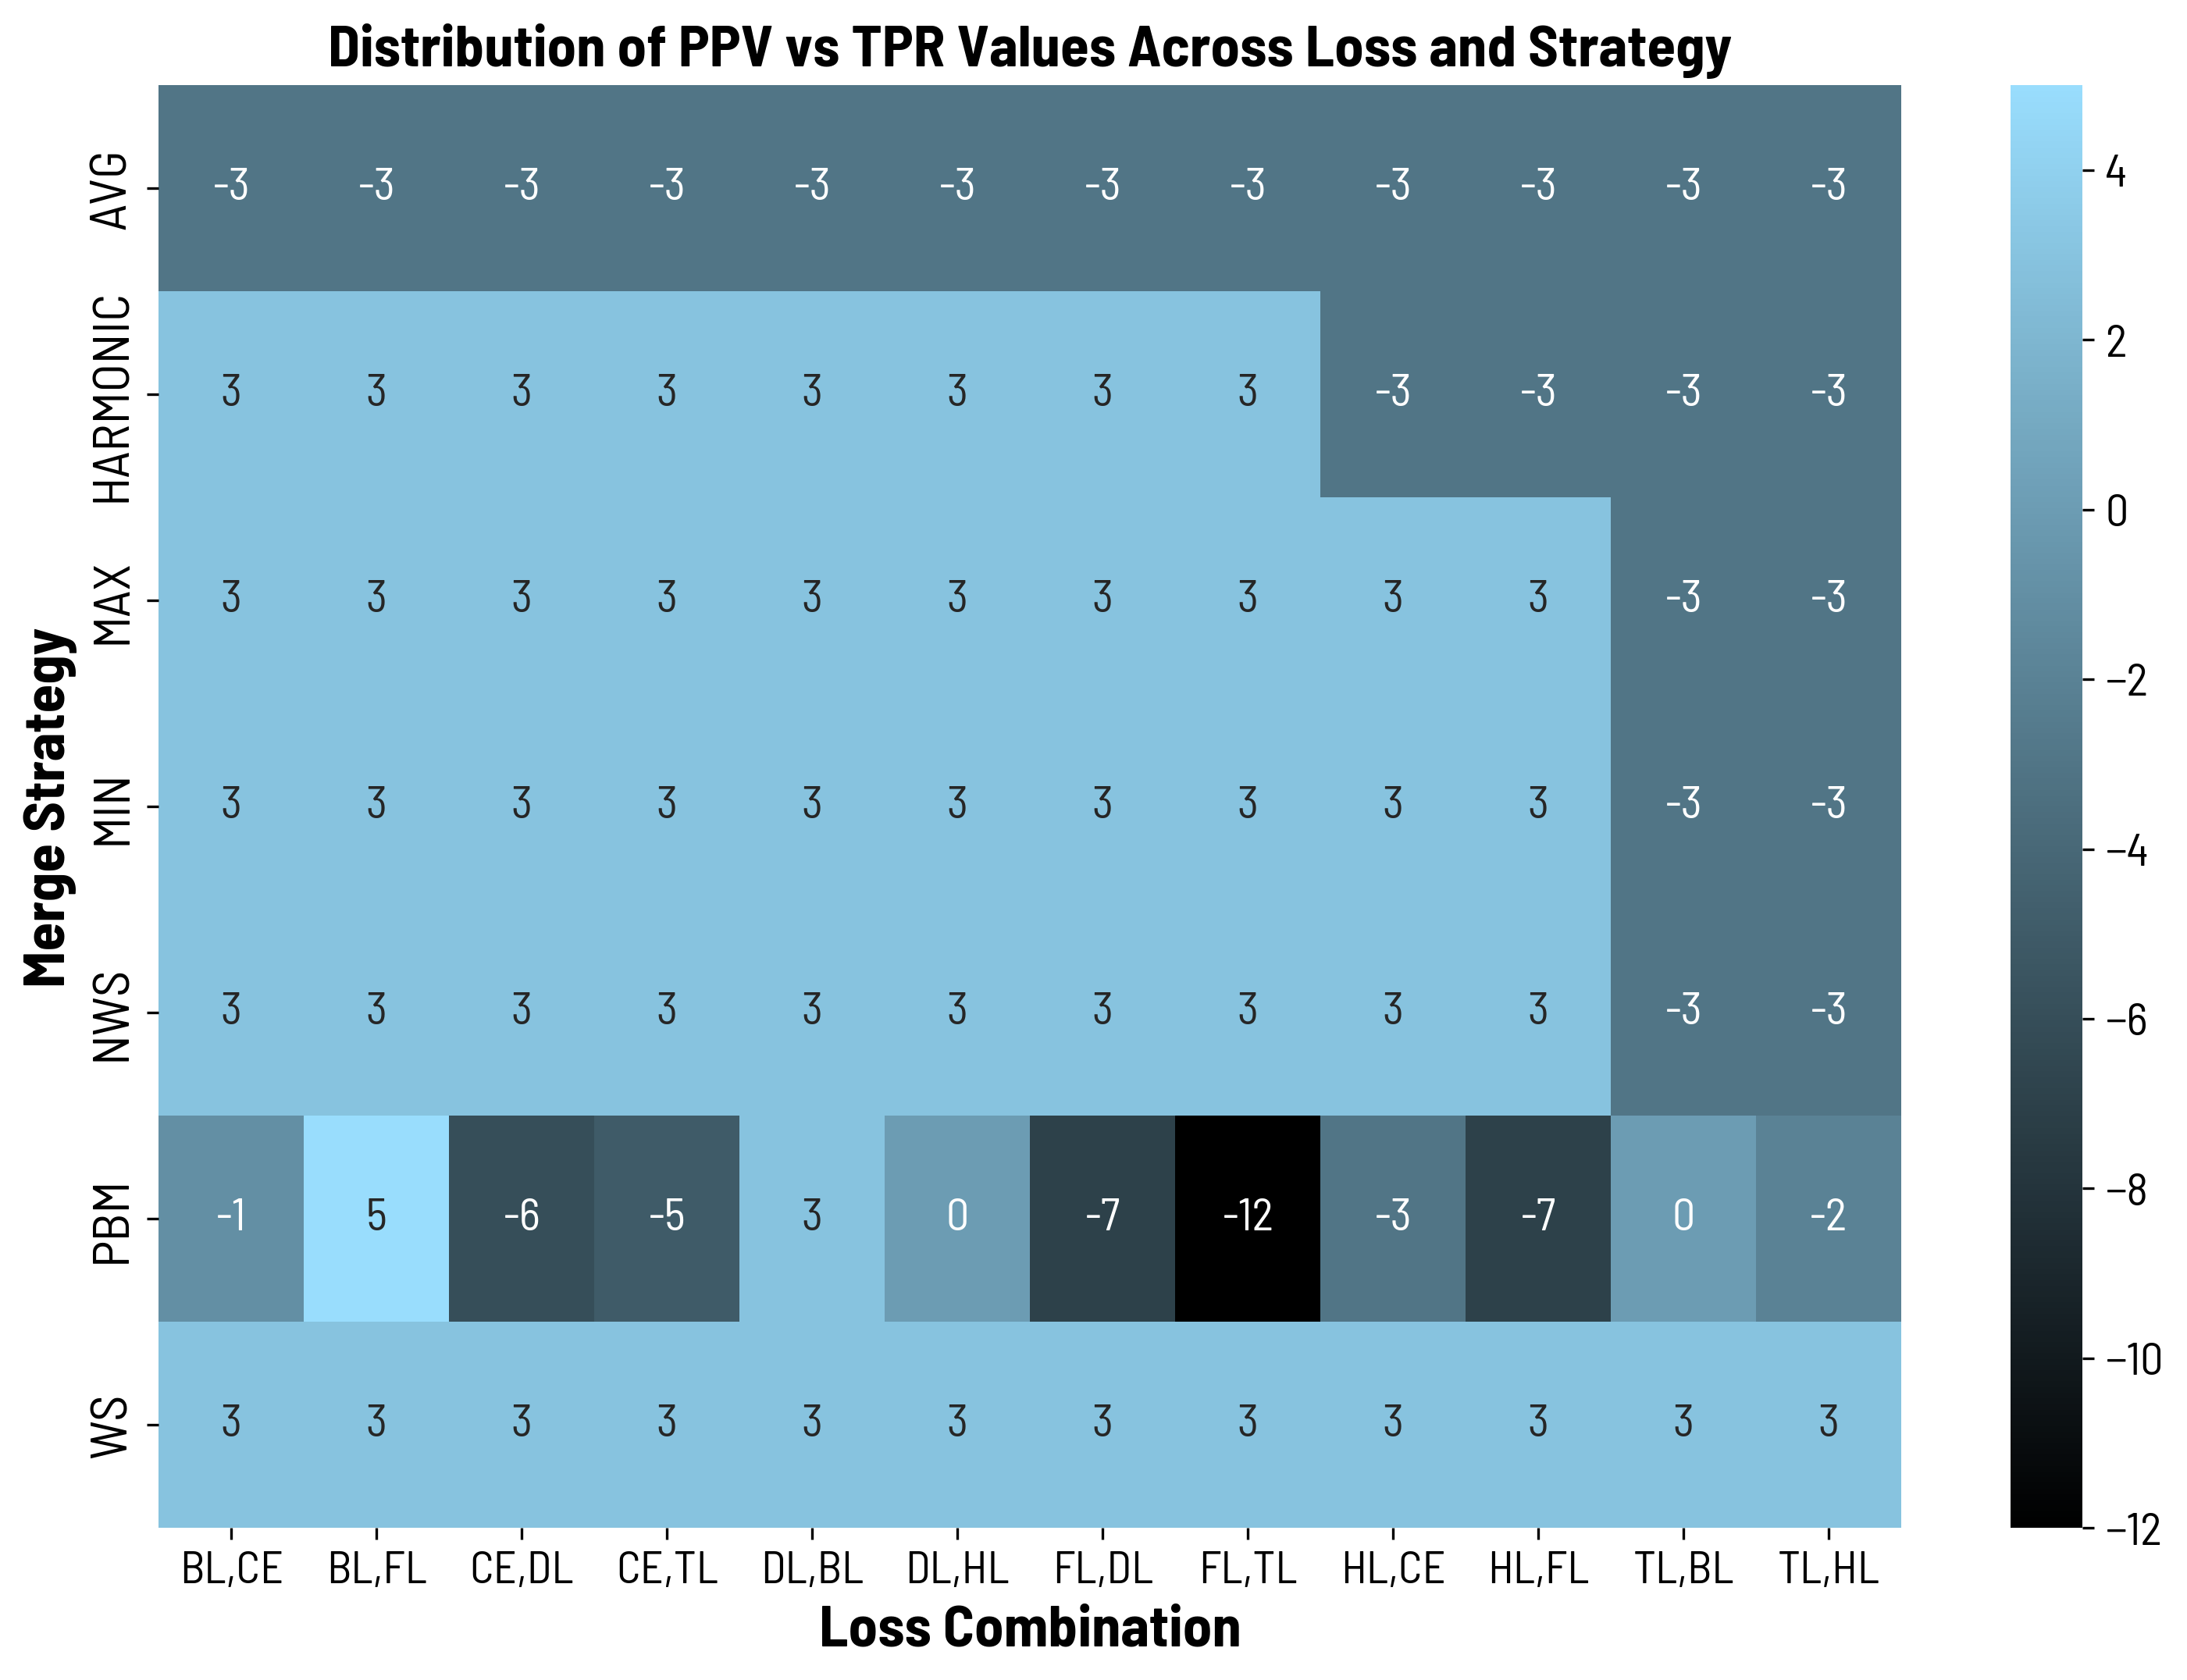
\includegraphics[width=\imgWidthcustom]{images/ppv_tpr_heatmap_double_melanoma.png}}
    \subfigure[Distribution of PPV vs. TPR for triple losses]{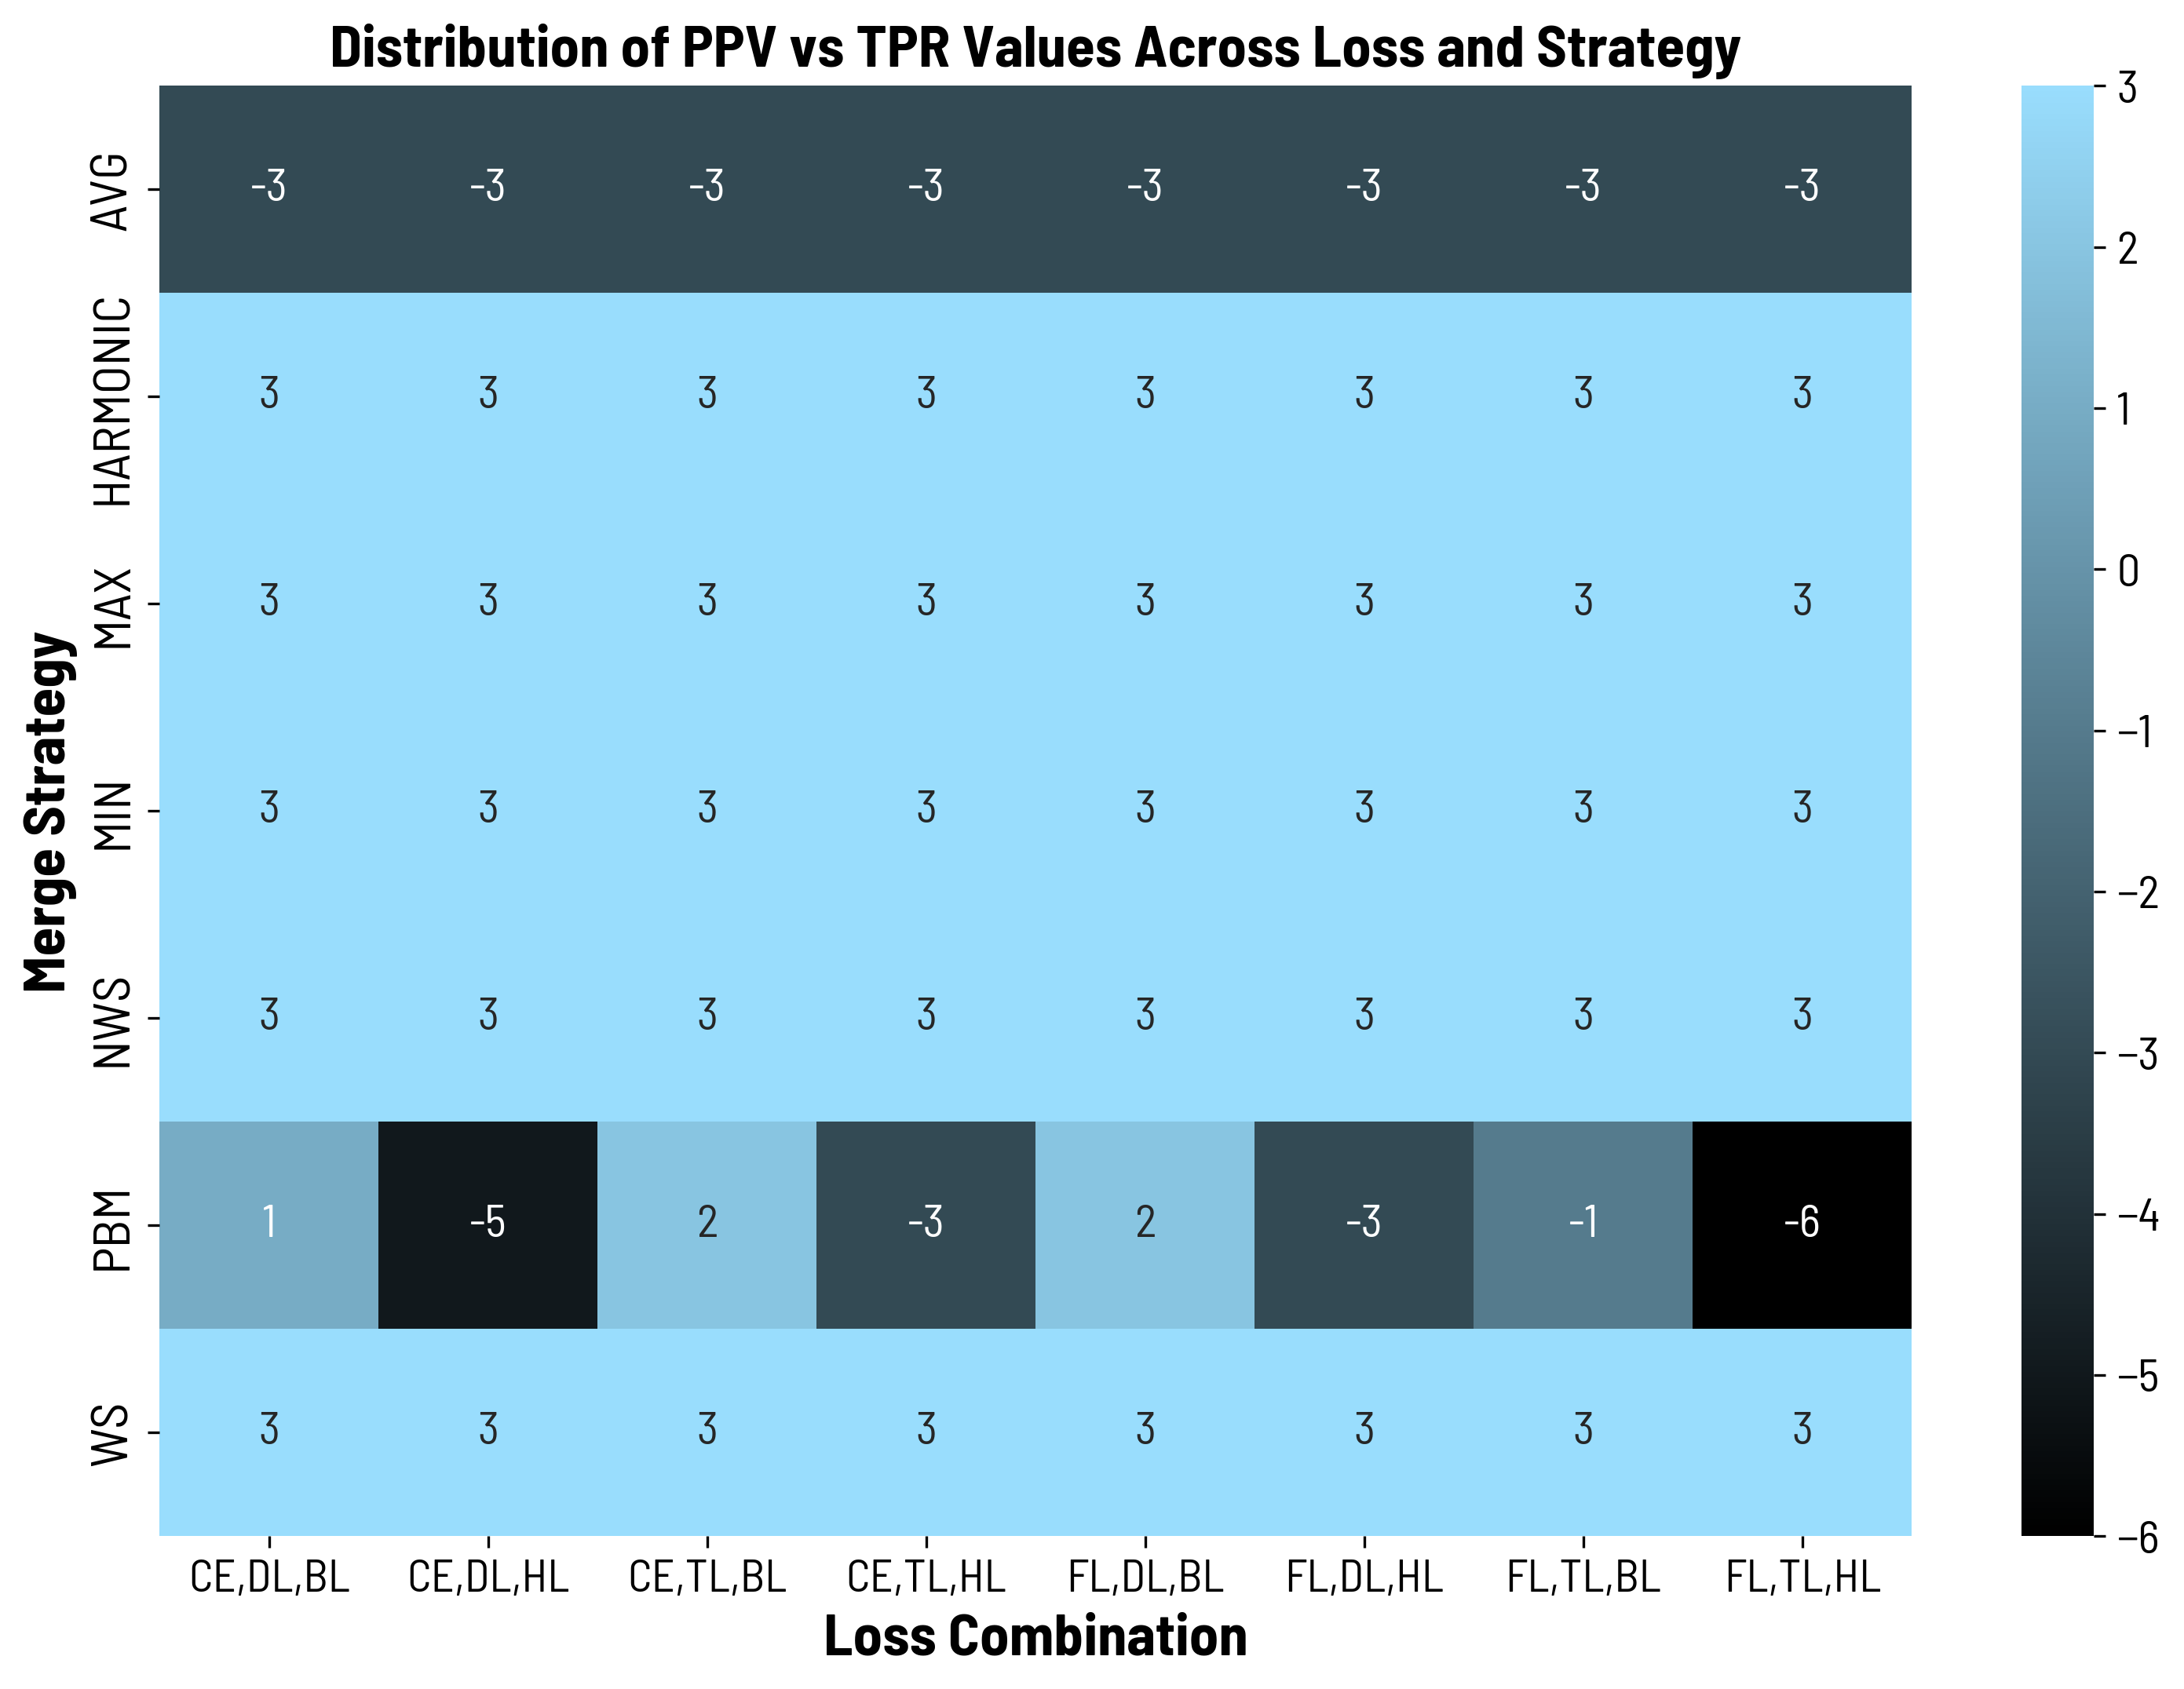
\includegraphics[width=\imgWidthcustom]{images/ppv_tpr_heatmap_triple_melanoma.png}}
    \caption[Distribution of PPV vs. TPR Values]{Heatmaps visualizing the relative prevalence as a difference map of PPV and TPR across various loss combinations and merge strategies. Each cell represents a unique combination. Positive values indicate a predominance of TPR, while negative values signify a predominance of PPV.}
    \label{ppv_vs_tpr_melanoma}
\end{figure}
\newpage

\subsection{Ablation study}
\begin{figure}[H]%[htbp]
    \centering
    \subfigure[Double Loss Combination for 100 \% Data Utilization]{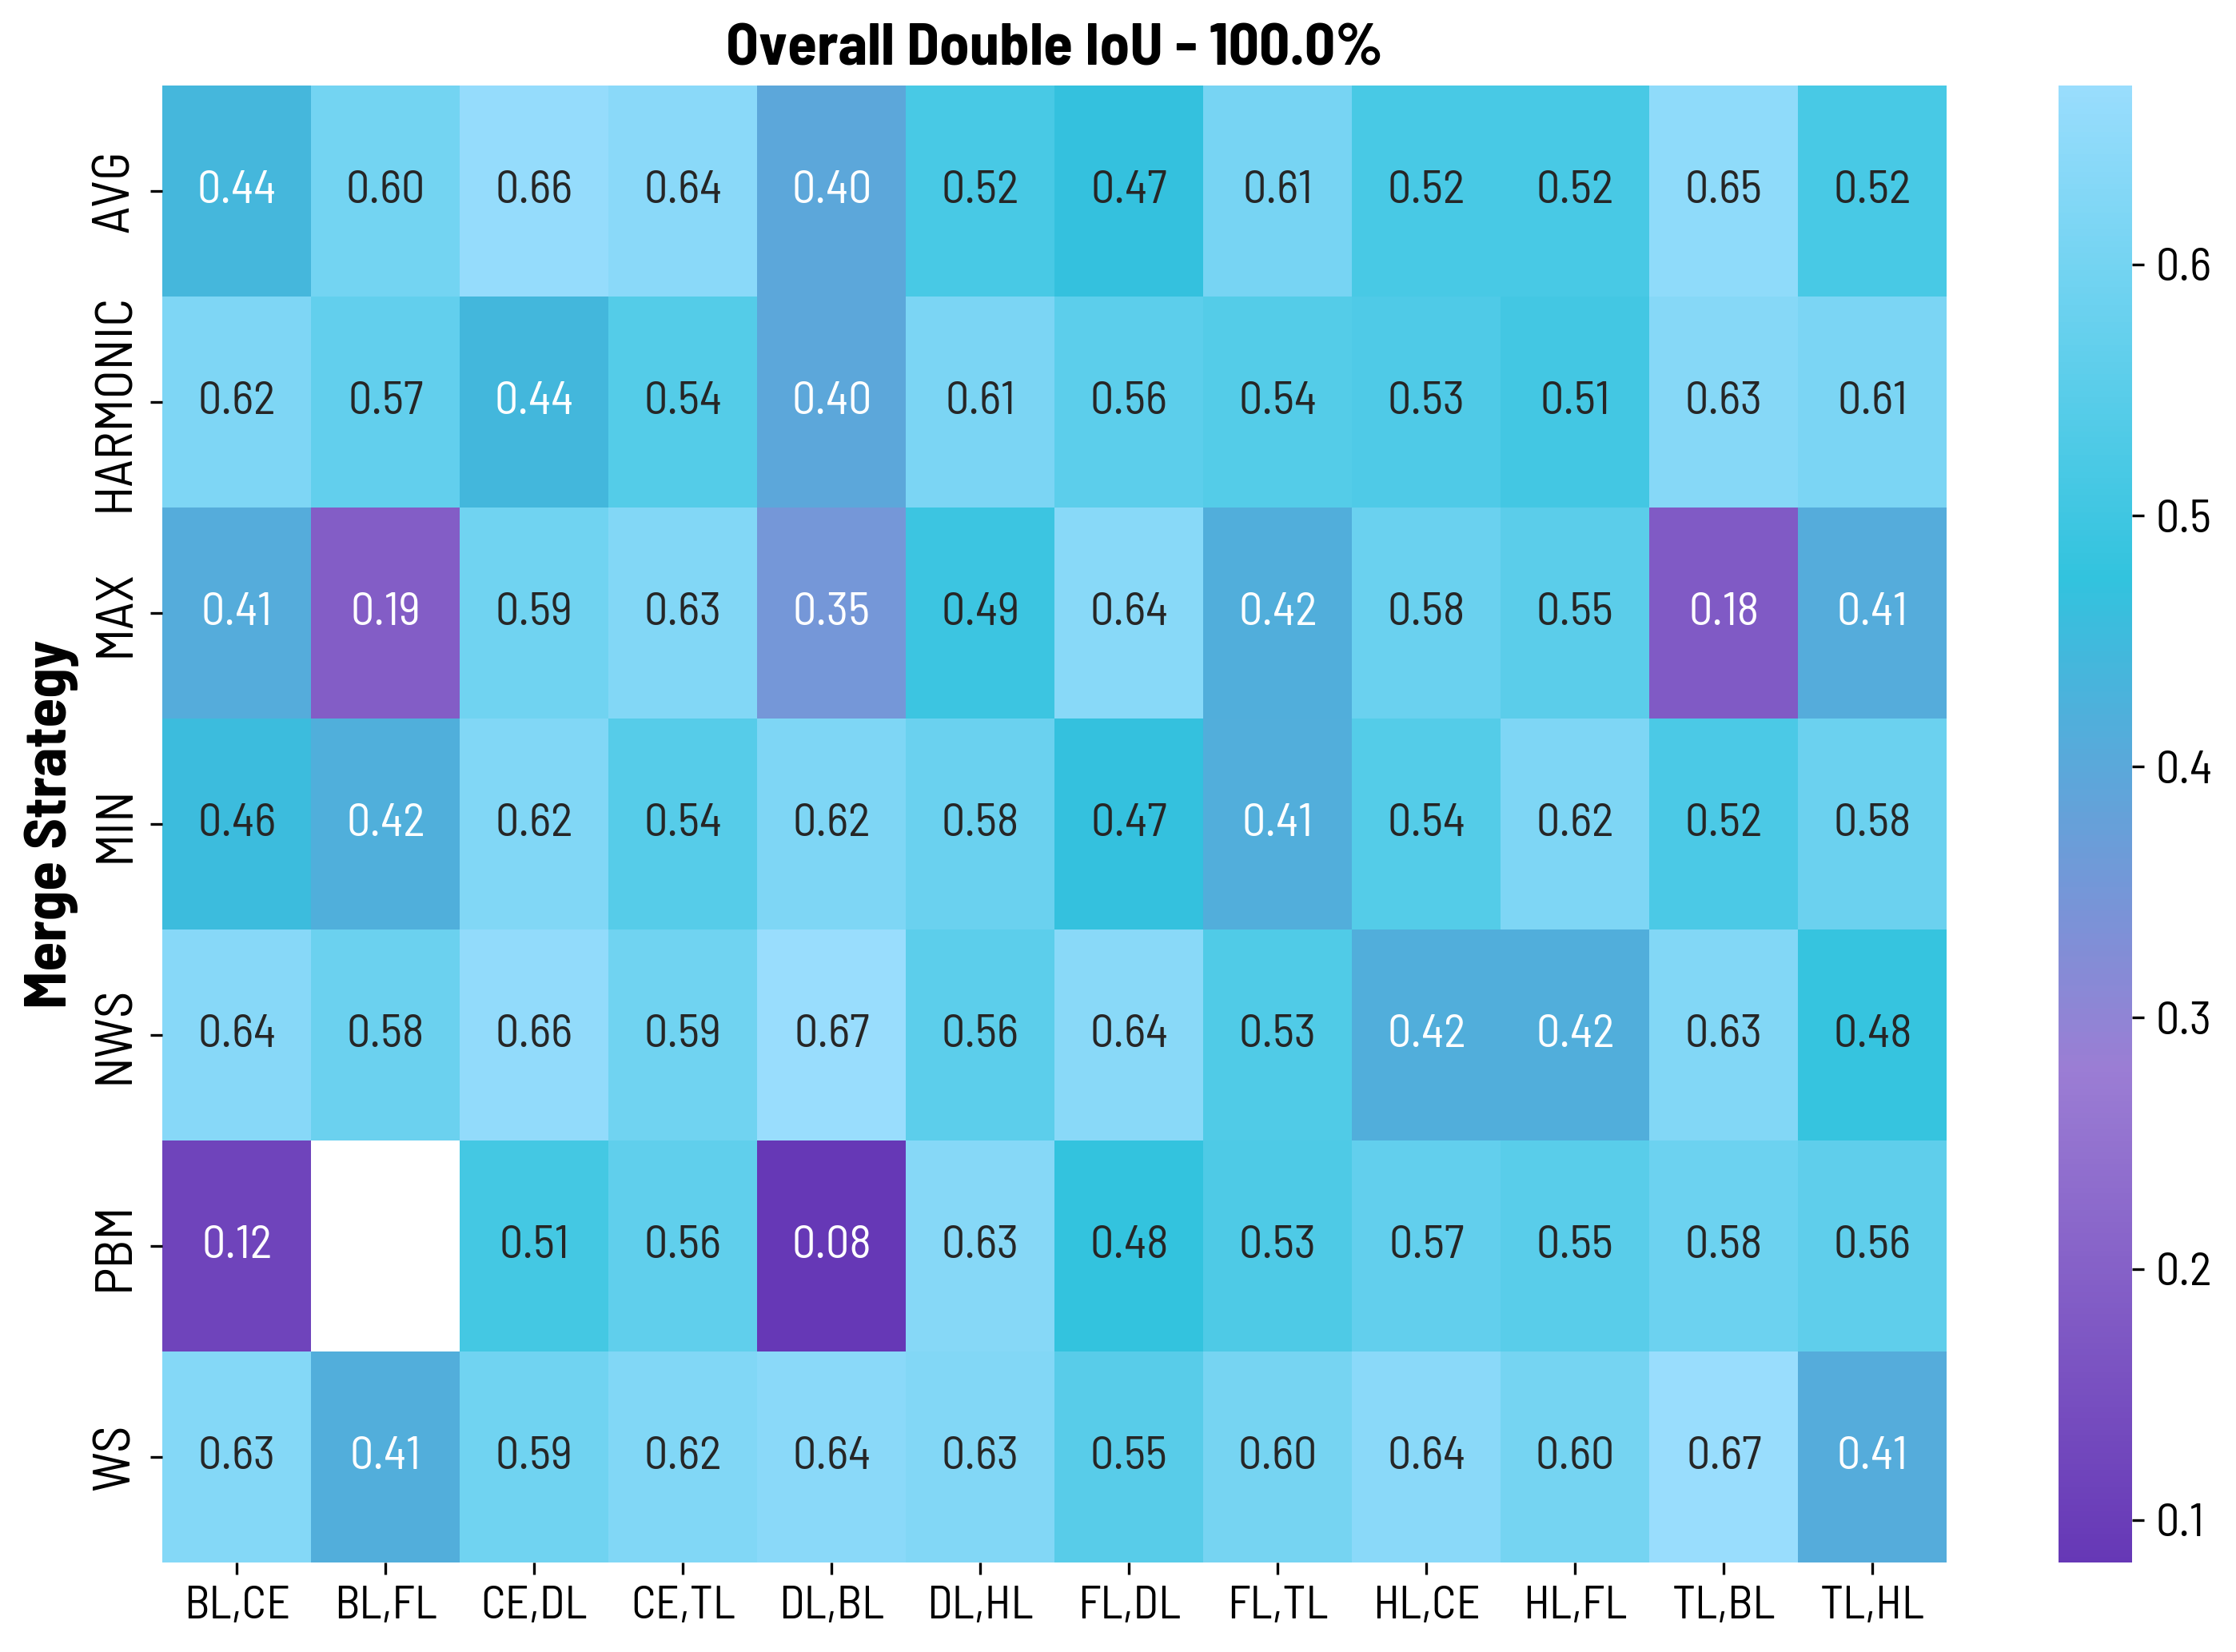
\includegraphics[width=\imgWidthcustom]{images/(1.0, 2)_ablation_summary_melanoma.png}}
    \subfigure[Triple Loss Combination for 100 \% Data Utilization]{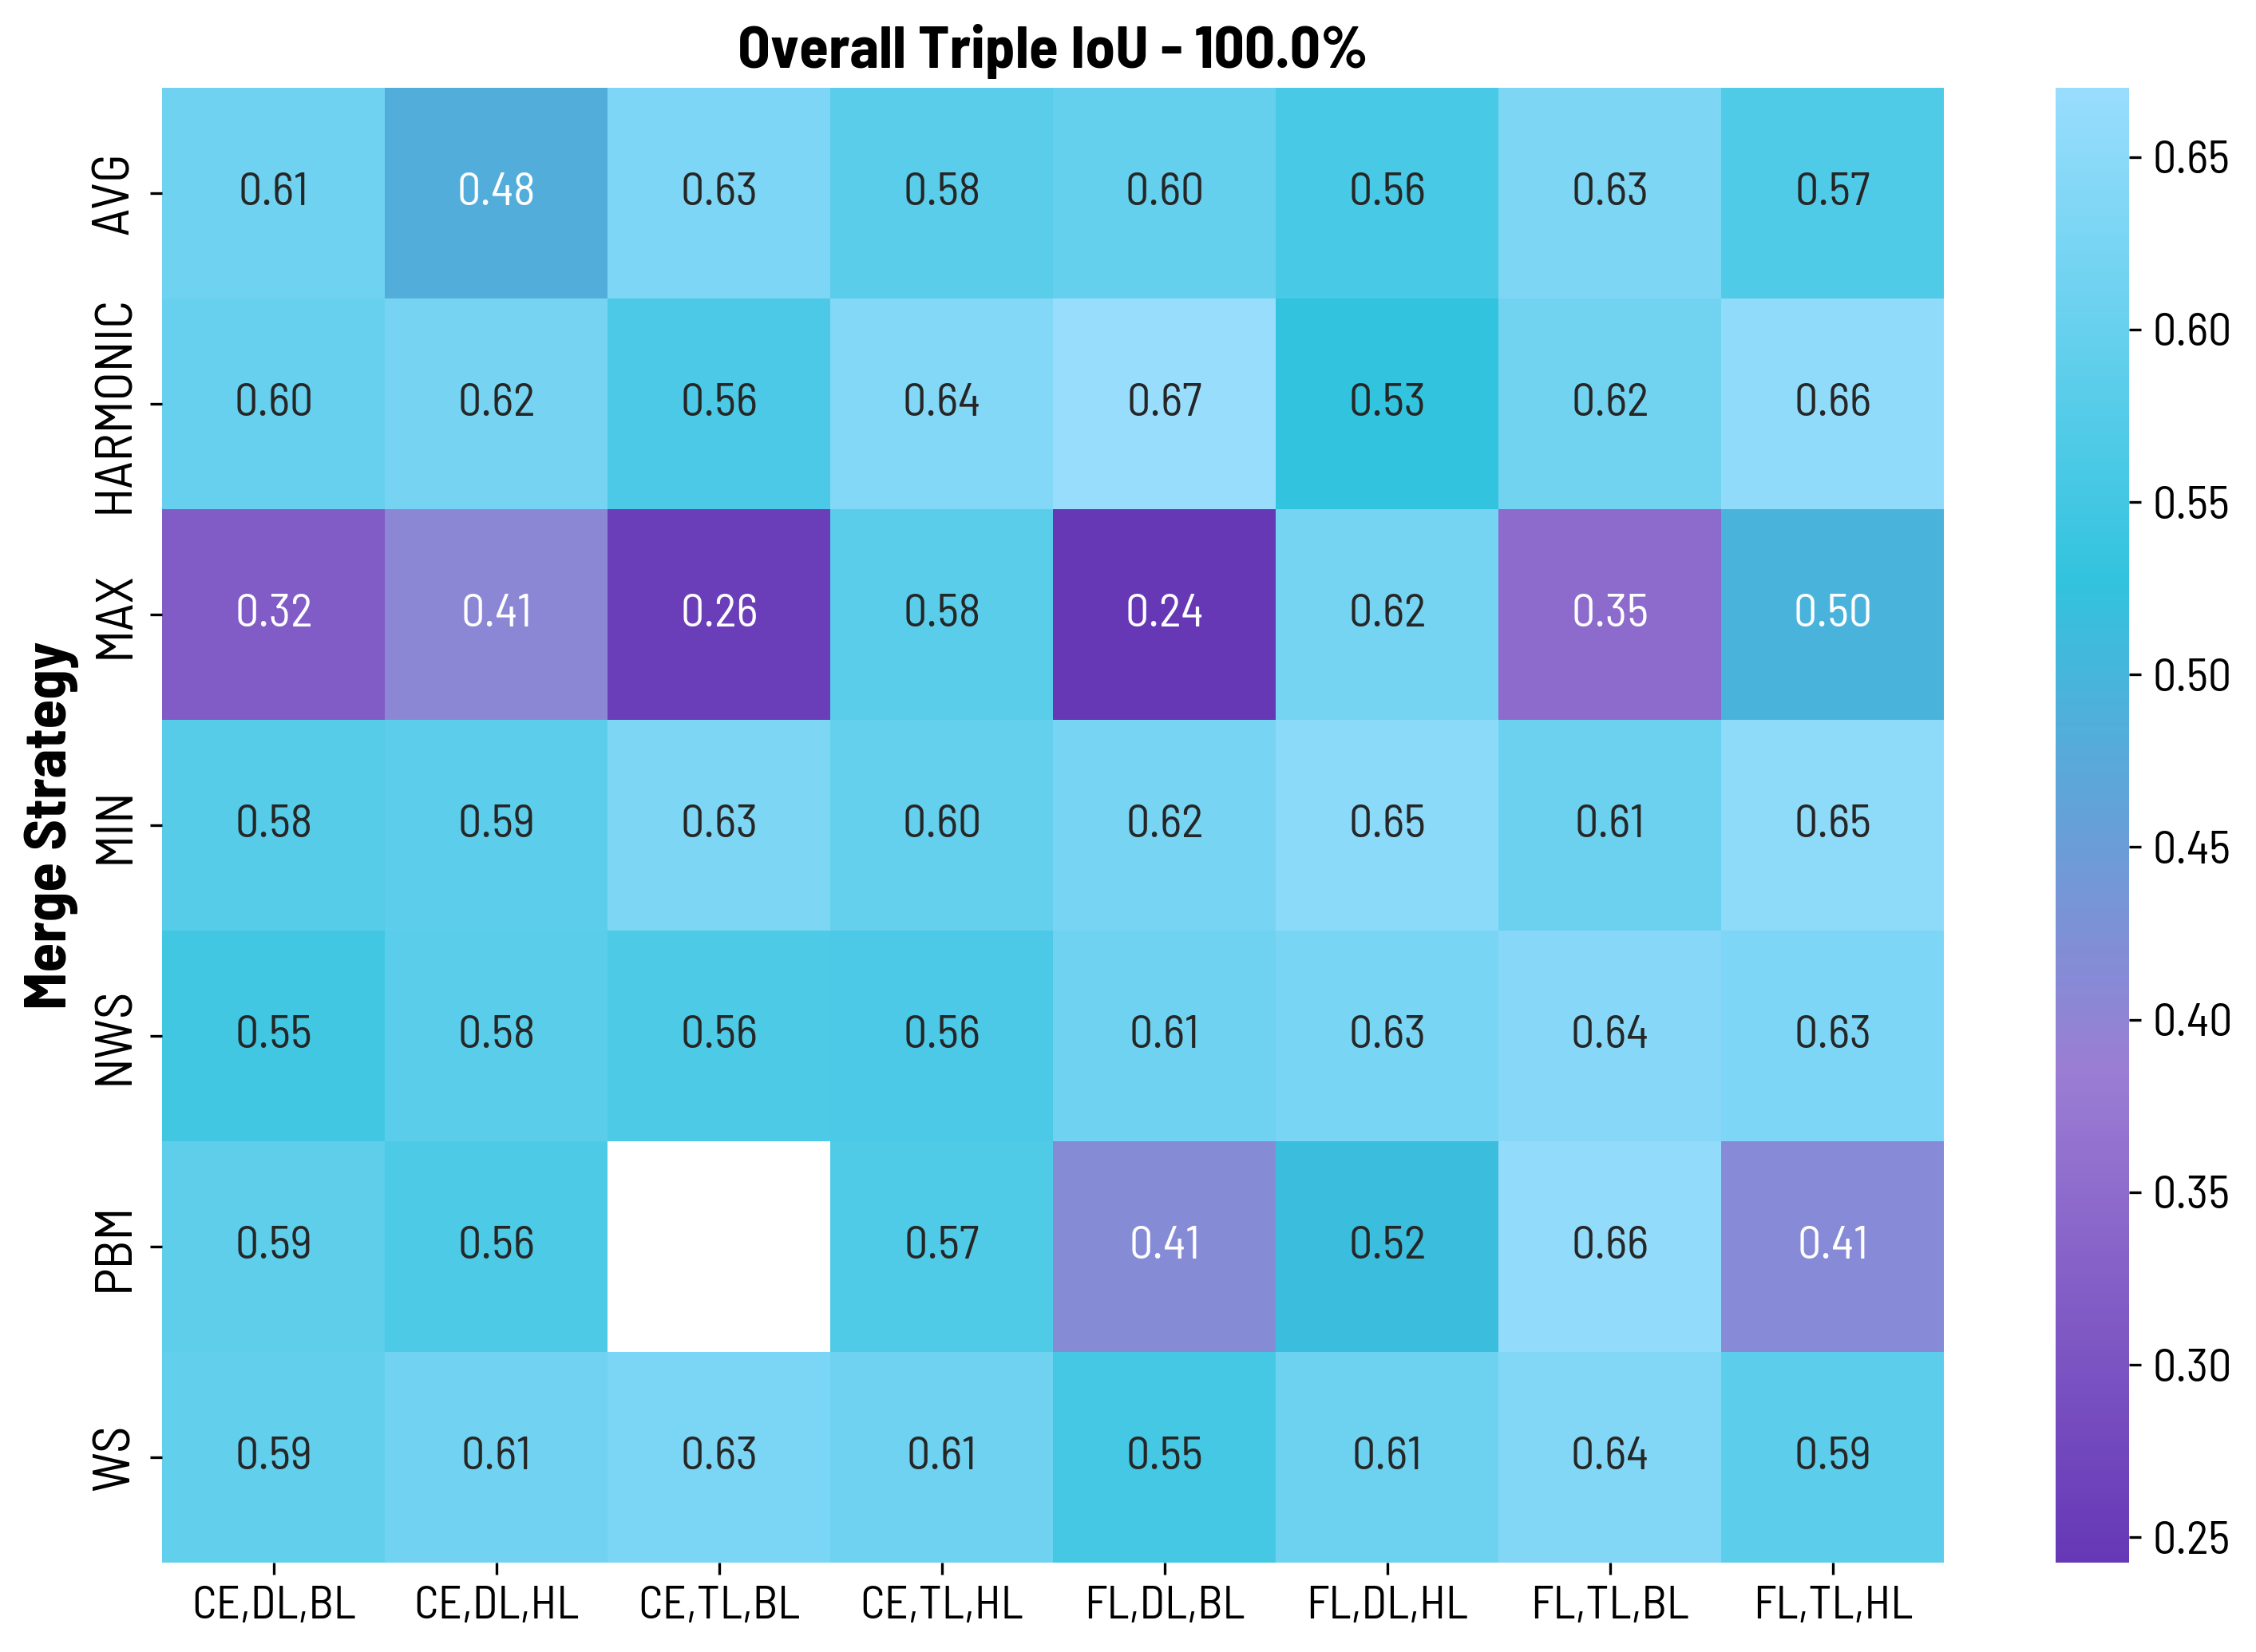
\includegraphics[width=\imgWidthcustom]{images/(1.0, 3)_ablation_summary_melanoma.png}}
    \subfigure[Double Loss Combination for 64 \% Data Utilization]{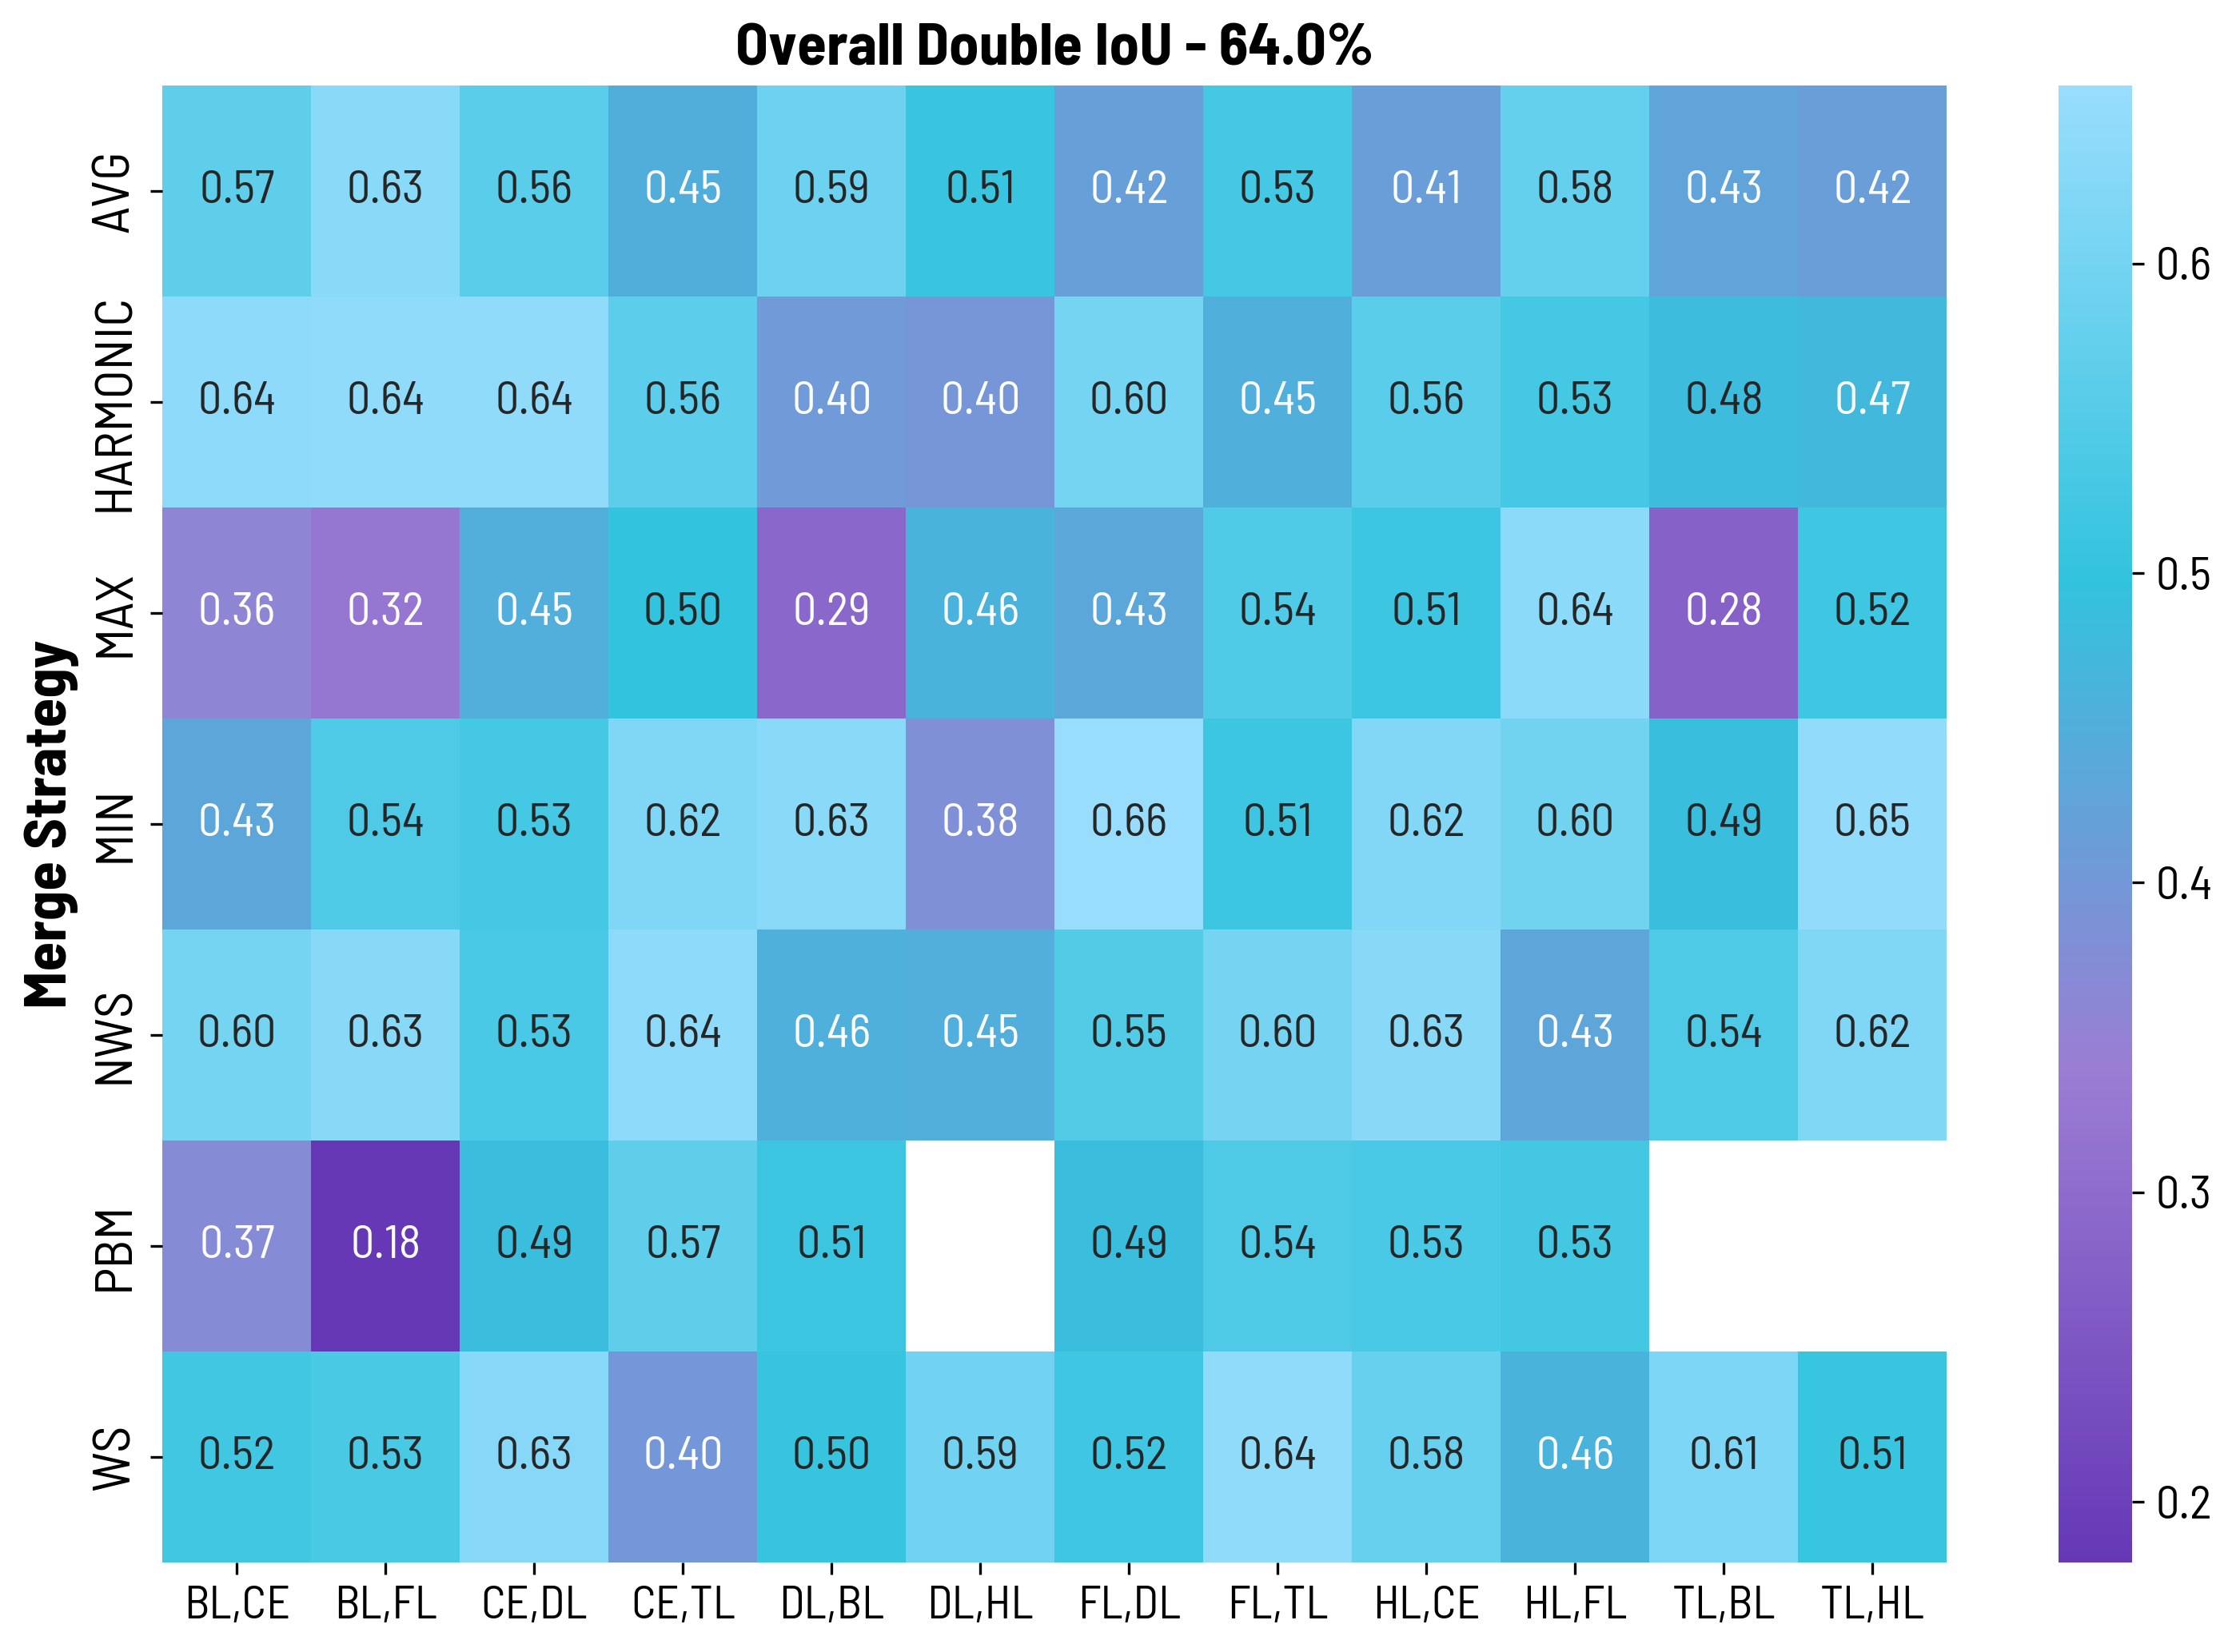
\includegraphics[width=\imgWidthcustom]{images/(0.64, 2)_ablation_summary_melanoma.png}}
    \subfigure[Triple Loss Combination for 64 \% Data Utilization]{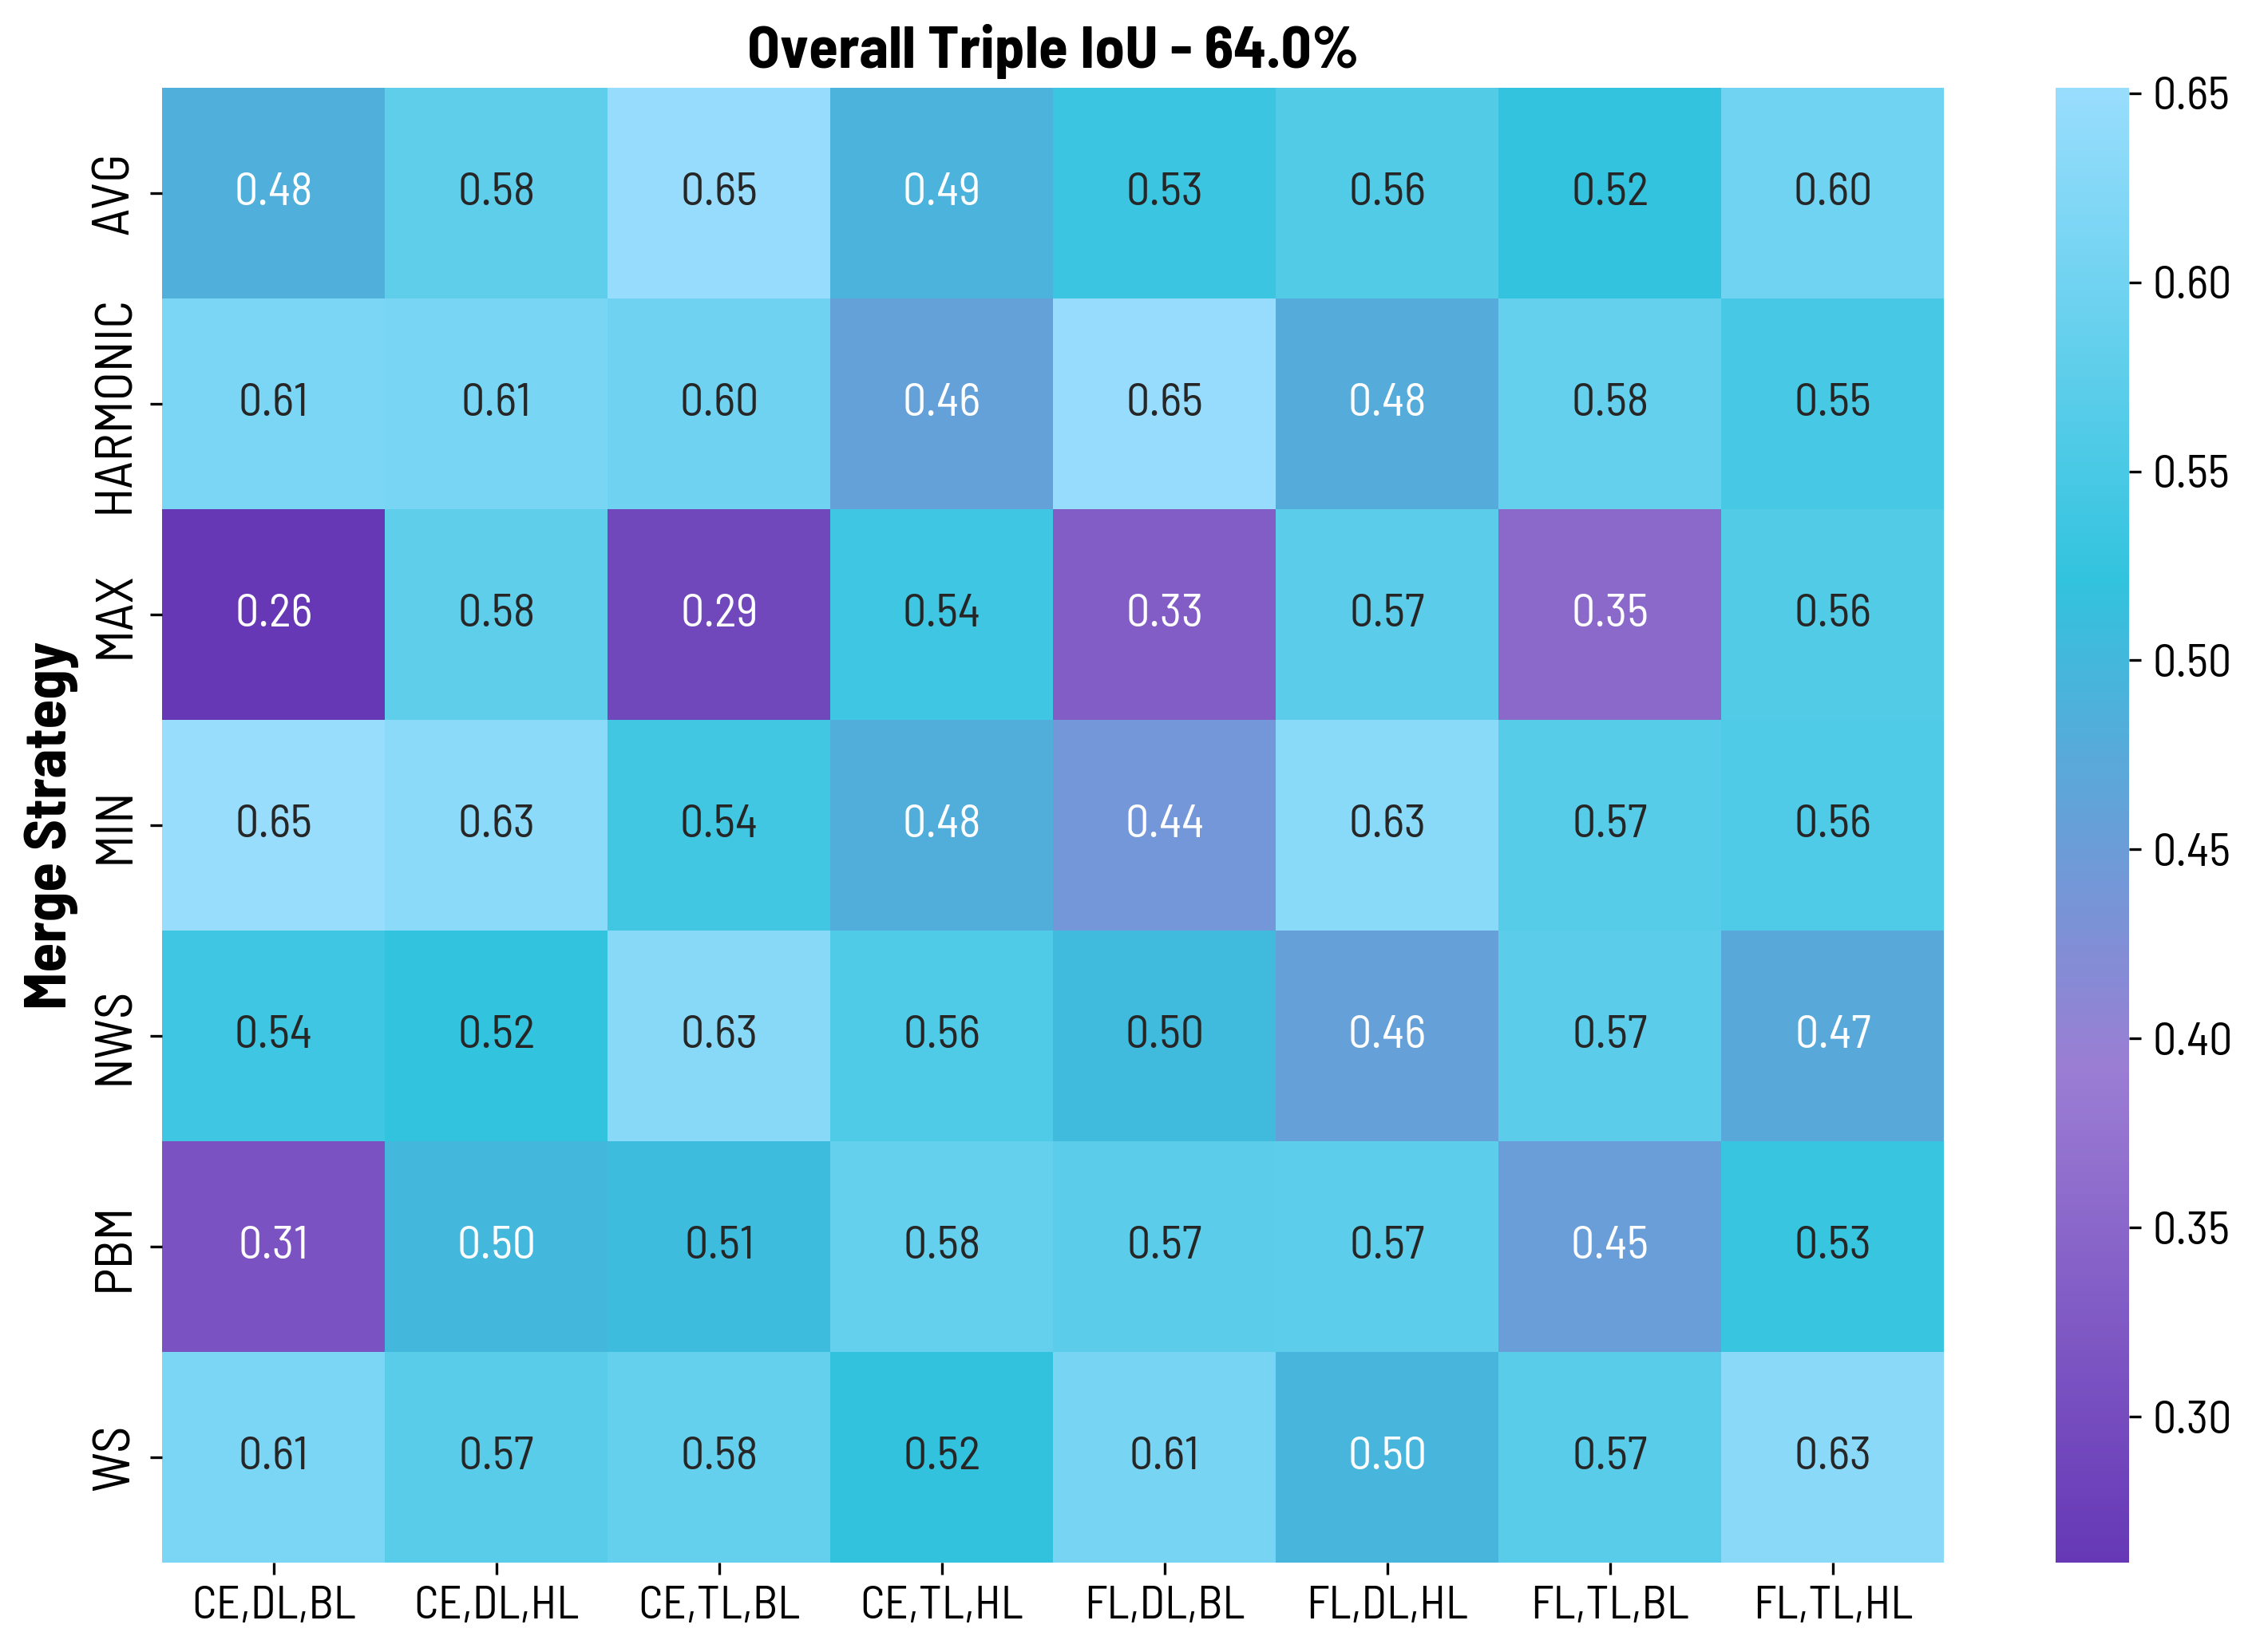
\includegraphics[width=\imgWidthcustom]{images/(0.64, 3)_ablation_summary_melanoma.png}}
    \subfigure[Double Loss Combination for 32 \% Data Utilization]{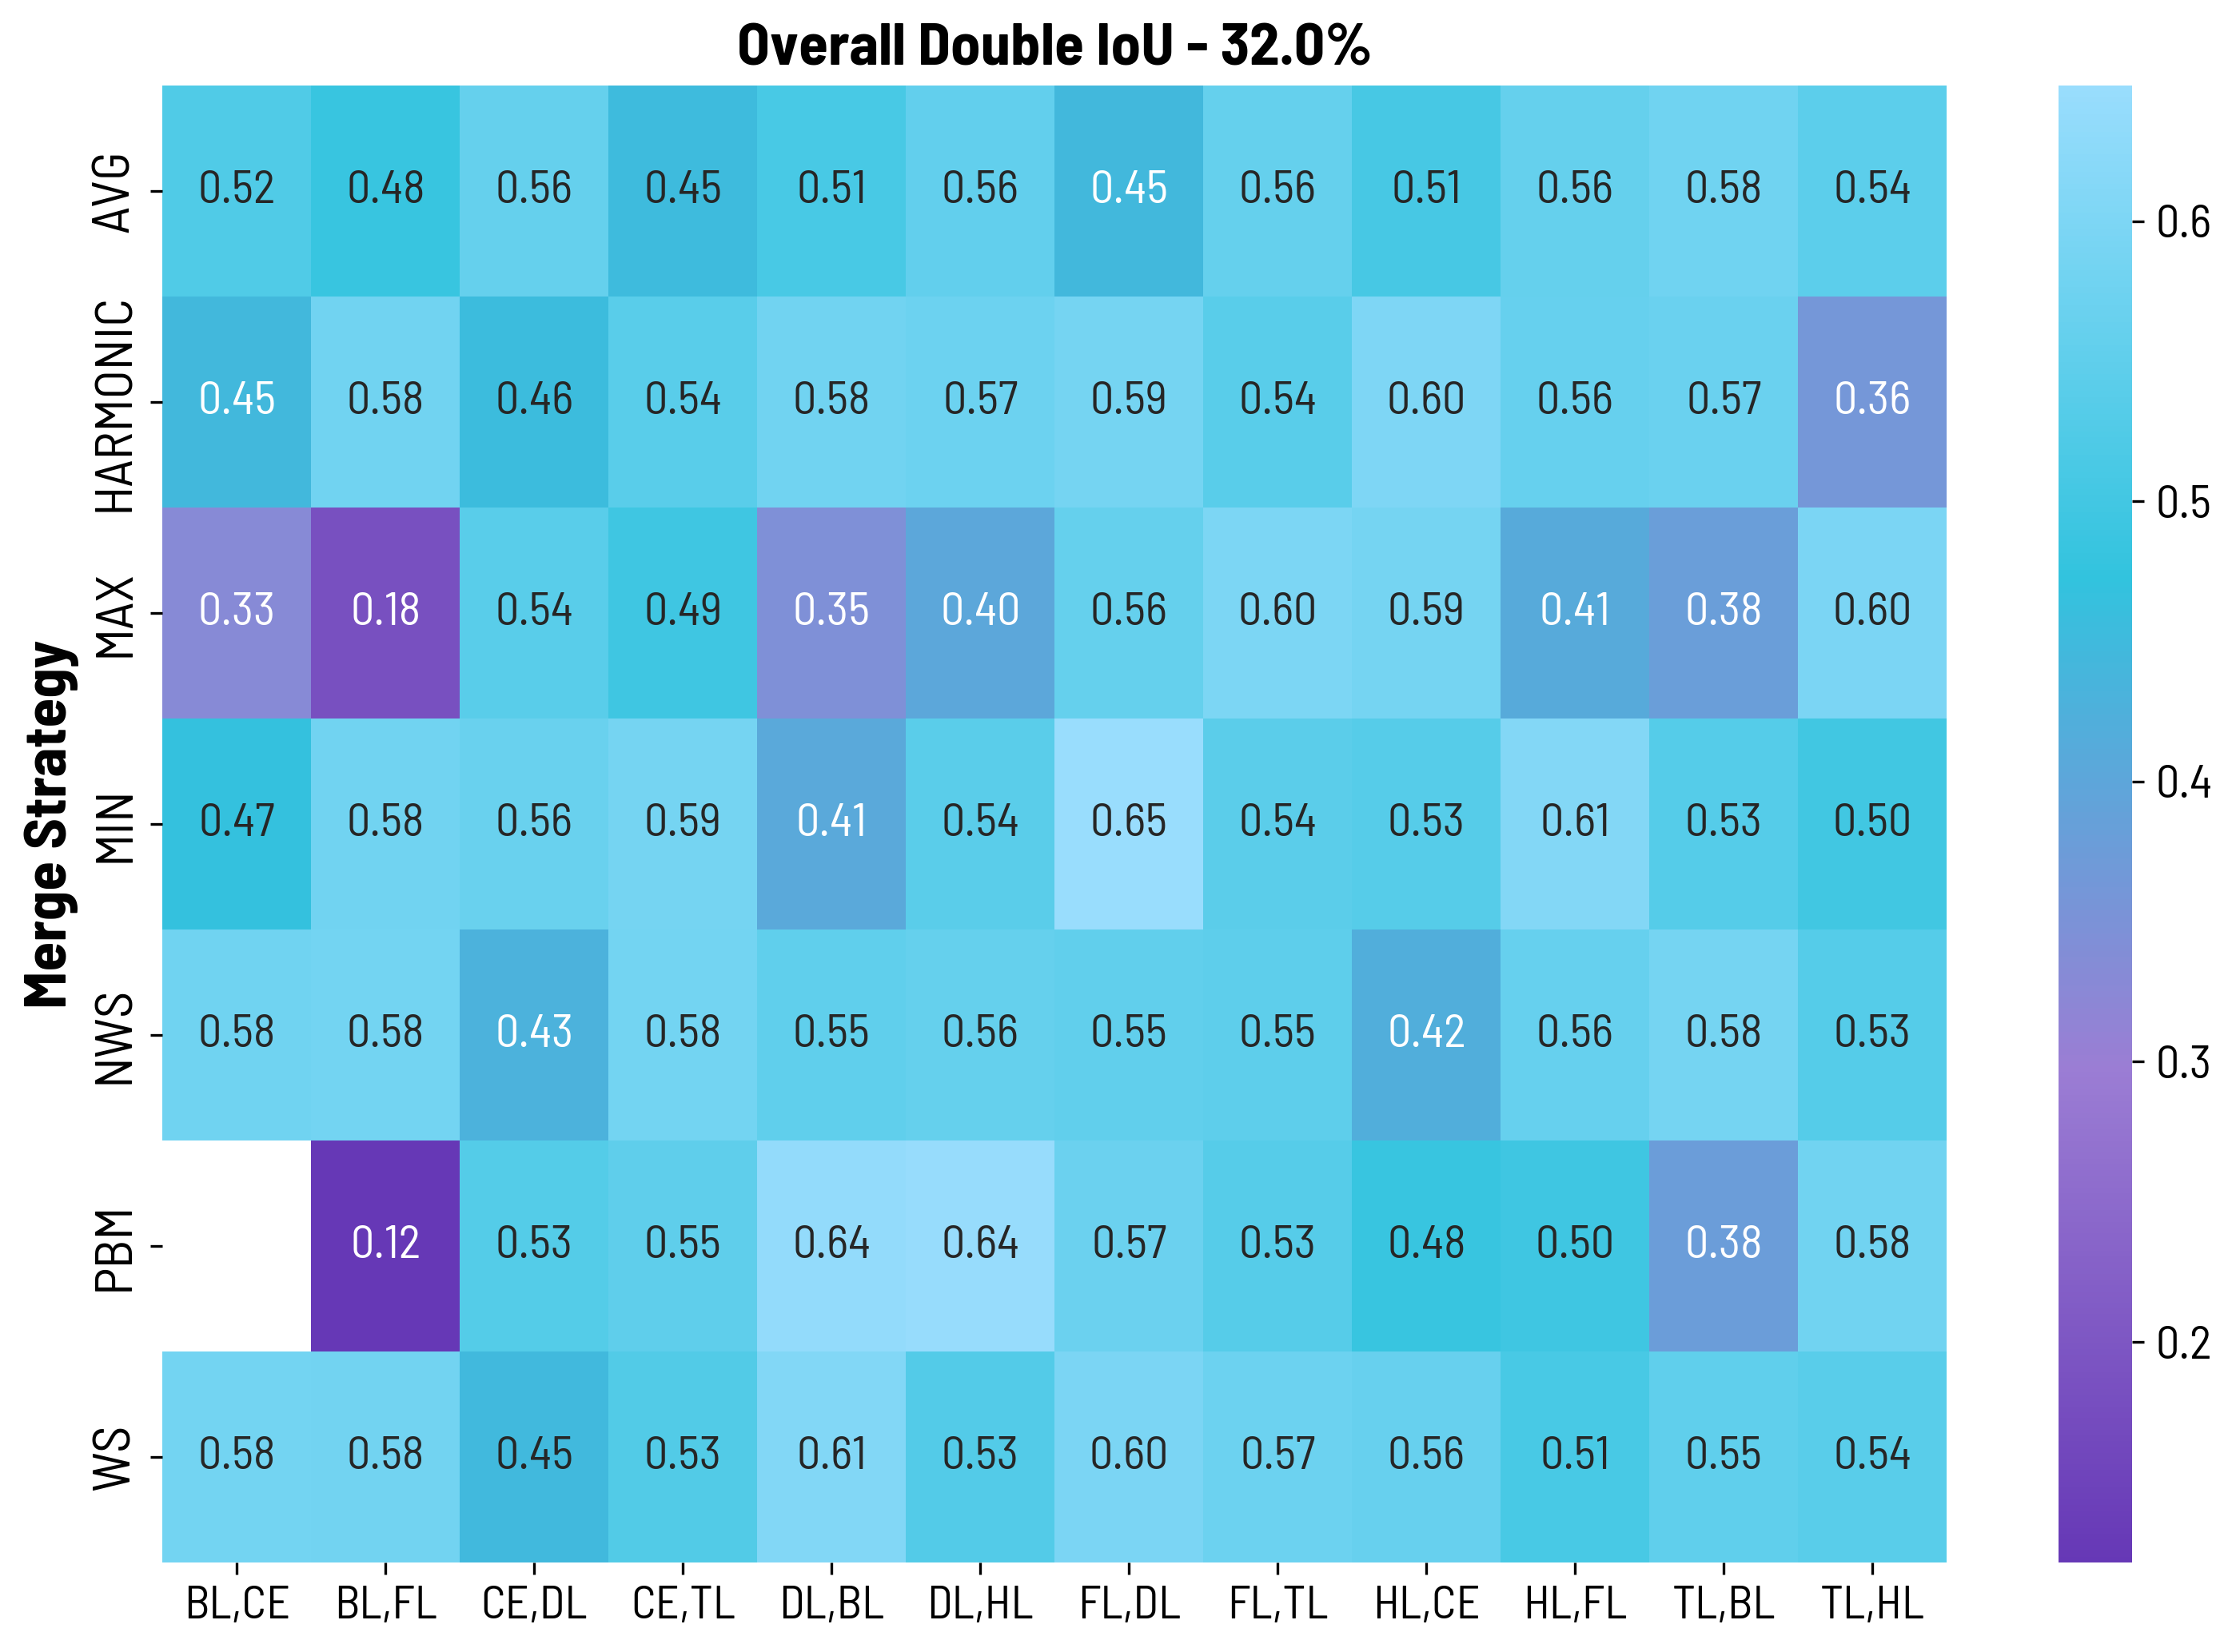
\includegraphics[width=\imgWidthcustom]{images/(0.32, 2)_ablation_summary_melanoma.png}}
    \subfigure[Triple Loss Combination for 32 \% Data Utilization]{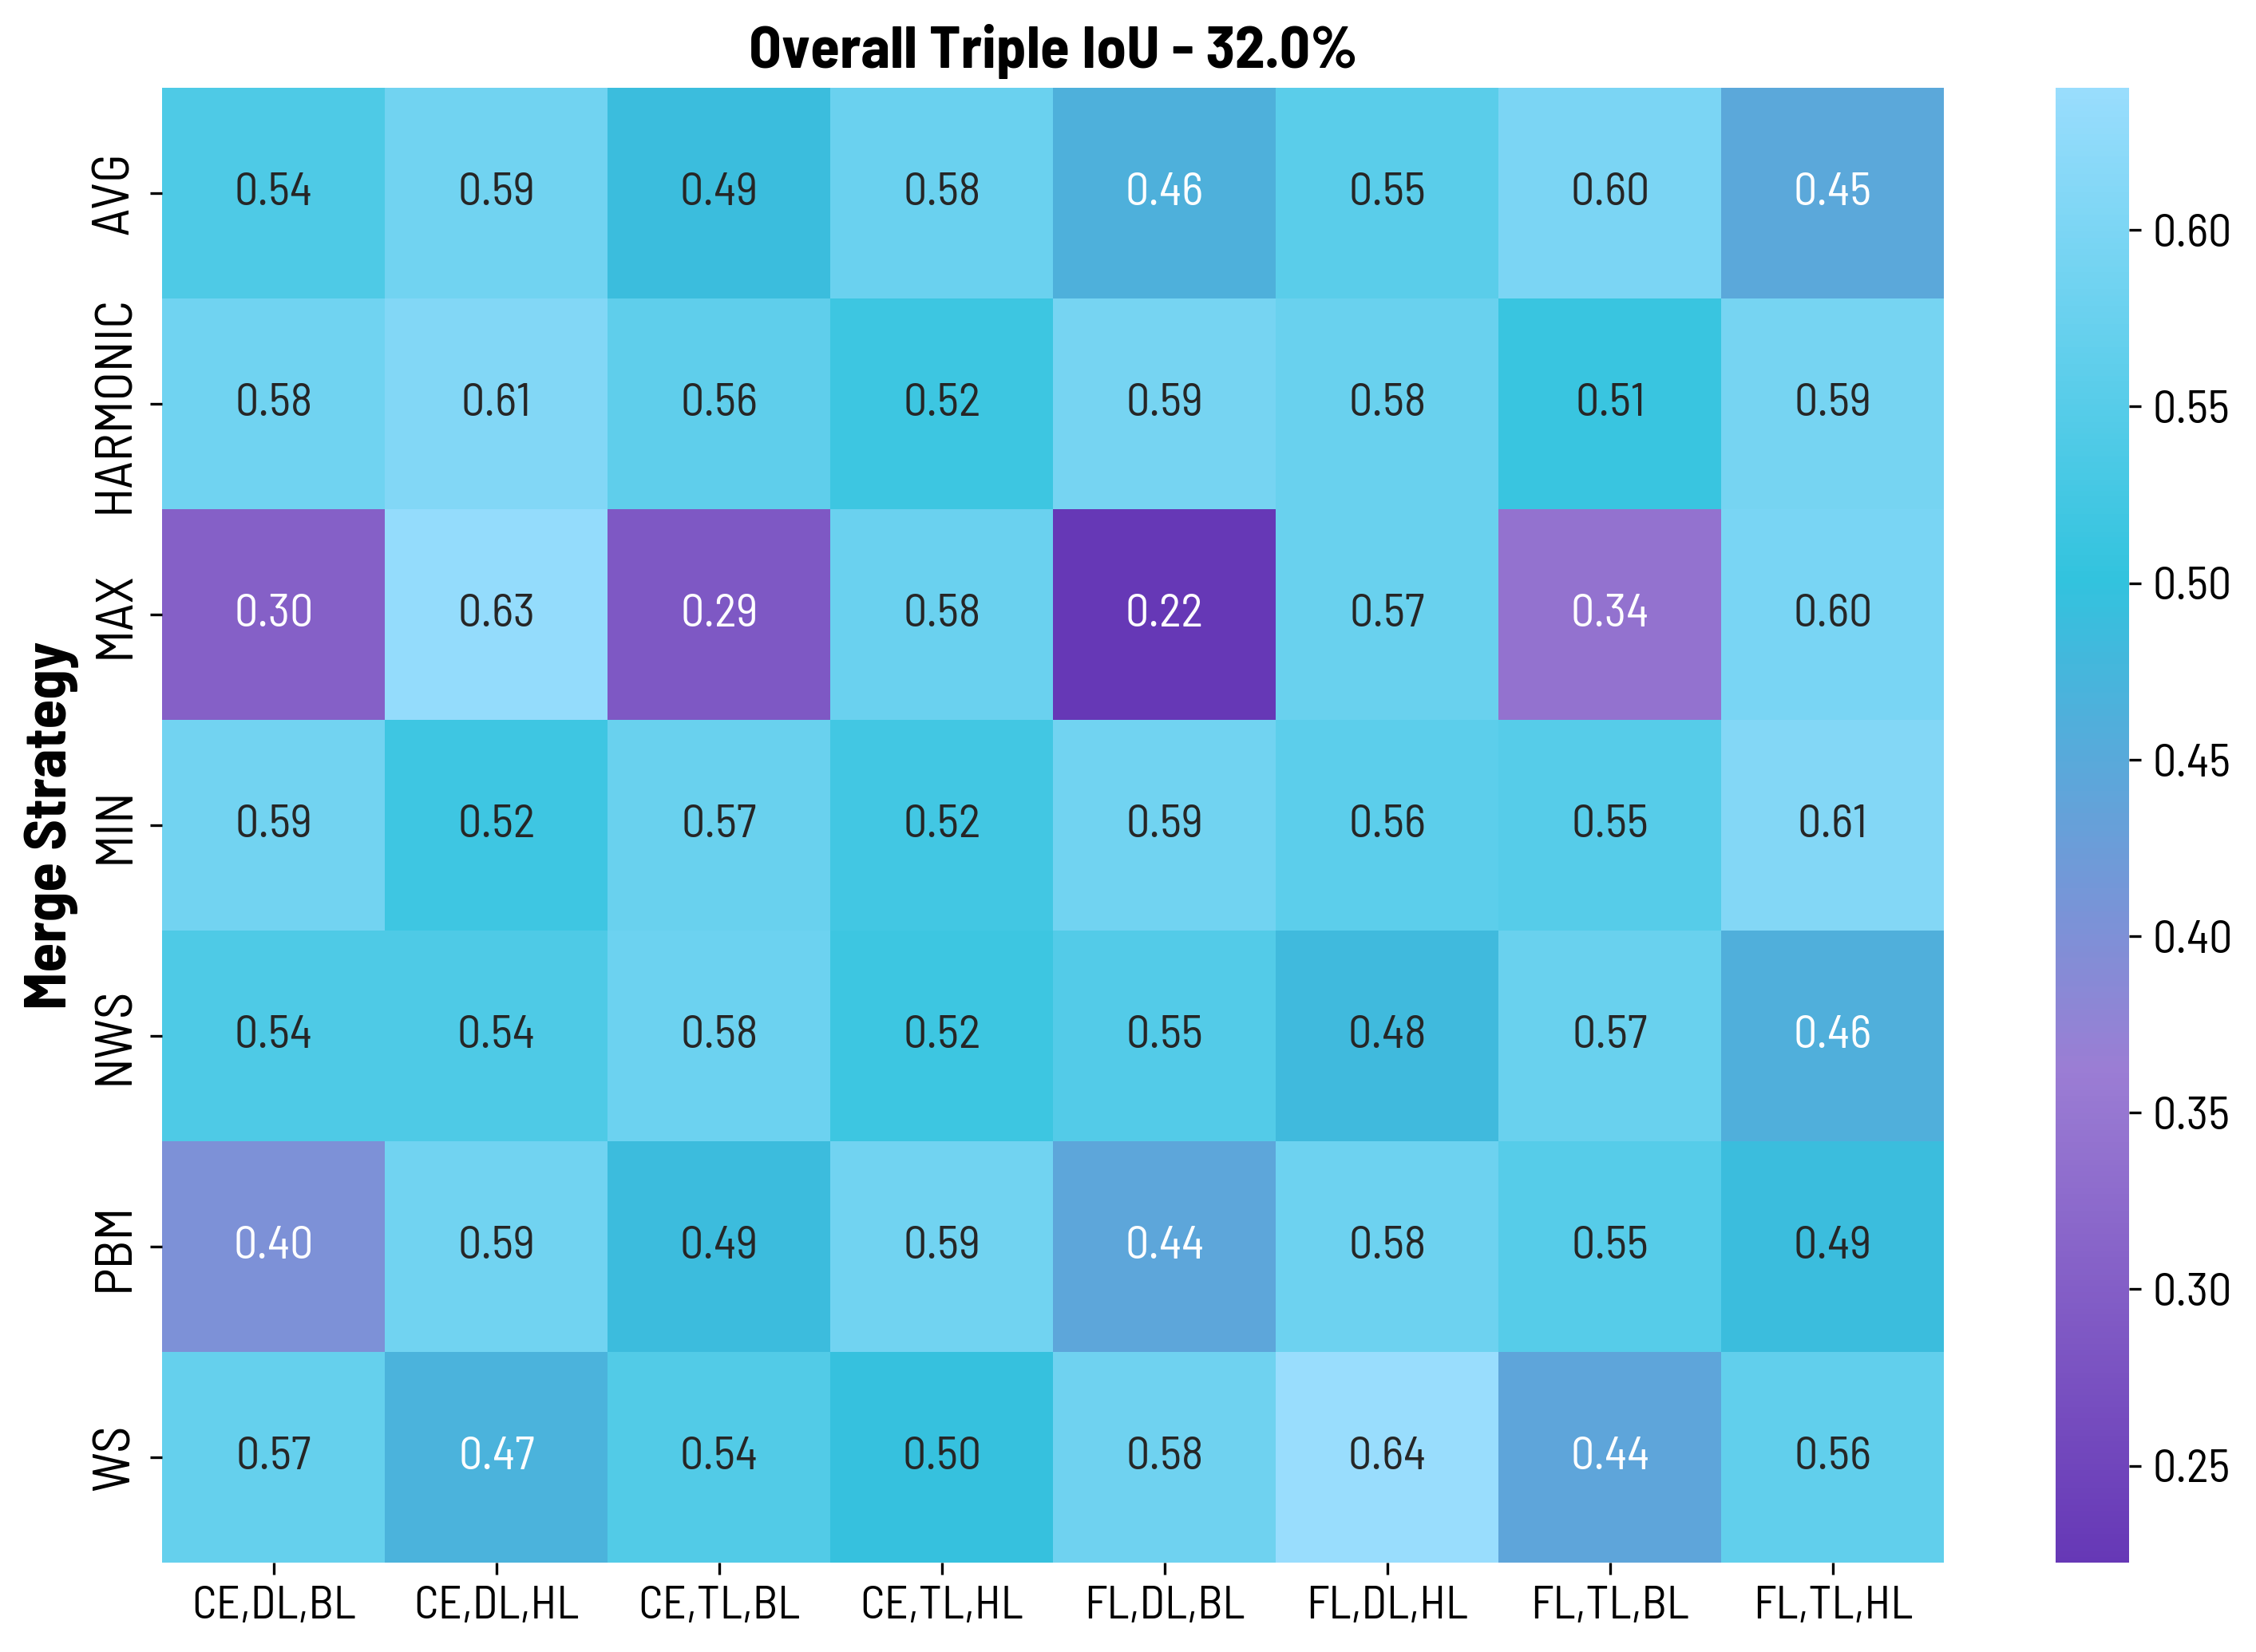
\includegraphics[width=\imgWidthcustom]{images/(0.32, 3)_ablation_summary_melanoma.png}}
    \caption[Overall results for different dataset sizes]{Overall results generated from different dataset sizes. The left column (a,c,e) illustrates results from double loss combinations, while the right column (b,d,f) depicts results from triple loss combinations.}
    \label{ablation_melanoma_heatmaps}
\end{figure}
\newpage


%----------------------------------------------------------------------------------------%
%---------------------------------------IDRID--------------------------------------------%
%----------------------------------------------------------------------------------------%
\section{Idrid}
\label{sec:supplementary_idrid}
\subsection{Baseline}
\label{subsec:baseline_idrid}
% Please add the following required packages to your document preamble:
% \usepackage{graphicx}
% \usepackage[table,xcdraw]{xcolor}
% If you use beamer only pass "xcolor=table" option, i.e. \documentclass[xcolor=table]{beamer}
\begin{table}[H]
  \centering
  \resizebox{\textwidth}{!}{%
  \begin{tabular}{ccc|l|l|l|l|l|l|l|l|l|c|}
  \hline
  \rowcolor[HTML]{000000} 
  \multicolumn{1}{|c|}{\cellcolor[HTML]{000000}{\color[HTML]{FFFFFF} No.}} &
    \multicolumn{1}{c|}{\cellcolor[HTML]{000000}{\color[HTML]{FFFFFF} R-time(m)}} &
    {\color[HTML]{FFFFFF} Loss type} &
    {\color[HTML]{FFFFFF} Loss} &
    {\color[HTML]{FFFFFF} Iou} &
    {\color[HTML]{FFFFFF} IoU 0} &
    {\color[HTML]{FFFFFF} IoU 1} &
    {\color[HTML]{FFFFFF} IoU 2} &
    {\color[HTML]{FFFFFF} IoU 3} &
    {\color[HTML]{FFFFFF} IoU 4} &
    {\color[HTML]{FFFFFF} PPV} &
    {\color[HTML]{FFFFFF} TPR} &
    {\color[HTML]{FFFFFF} PPV vs. TPR} \\ \hline
  \multicolumn{1}{|c|}{1} &
    \multicolumn{1}{c|}{37} &
    \cellcolor[HTML]{6638B6}{\color[HTML]{FFFFFF} DB} &
    CE &
    0.367 &
    0.961 &
    0.002 &
    0.234 &
    0.002 &
    0.634 &
    0.520 &
    0.435 &
    PPV \\ \hline
  \multicolumn{1}{|c|}{2} &
    \multicolumn{1}{c|}{44} &
    \cellcolor[HTML]{6638B6}{\color[HTML]{FFFFFF} DB} &
    CE &
    0.364 &
    0.954 &
    0.002 &
    0.290 &
    0.011 &
    0.561 &
    0.565 &
    0.429 &
    PPV \\ \hline
  \multicolumn{1}{|c|}{3} &
    \multicolumn{1}{c|}{40} &
    \cellcolor[HTML]{6638B6}{\color[HTML]{FFFFFF} DB} &
    CE &
    0.348 &
    0.958 &
    0.042 &
    0.289 &
    0.000 &
    0.449 &
    0.525 &
    0.408 &
    PPV \\ \hline
   &
     &
    {\color[HTML]{FFFFFF} } &
    {\color[HTML]{000000} \textit{\textbf{CE Result}}} &
    {\color[HTML]{000000} \textit{\textbf{0.359}}} &
    {\color[HTML]{000000} \textit{\textbf{0.958}}} &
    {\color[HTML]{000000} \textit{\textbf{0.015}}} &
    {\color[HTML]{000000} \textit{\textbf{0.271}}} &
    {\color[HTML]{000000} \textit{\textbf{0.004}}} &
    {\color[HTML]{000000} \textit{\textbf{0.548}}} &
    {\color[HTML]{000000} \textit{\textbf{0.537}}} &
    {\color[HTML]{000000} \textit{\textbf{0.424}}} &
    \textbf{PPV} \\ \hline
  \multicolumn{1}{|c|}{4} &
    \multicolumn{1}{c|}{35} &
    \cellcolor[HTML]{6638B6}{\color[HTML]{FFFFFF} DB} &
    FL &
    0.361 &
    0.949 &
    0.003 &
    0.289 &
    0.027 &
    0.539 &
    0.602 &
    0.431 &
    PPV \\ \hline
  \multicolumn{1}{|c|}{5} &
    \multicolumn{1}{c|}{42} &
    \cellcolor[HTML]{6638B6}{\color[HTML]{FFFFFF} DB} &
    FL &
    0.301 &
    0.940 &
    0.002 &
    0.258 &
    0.023 &
    0.282 &
    0.522 &
    0.374 &
    PPV \\ \hline
  \multicolumn{1}{|c|}{6} &
    \multicolumn{1}{c|}{35} &
    \cellcolor[HTML]{6638B6}{\color[HTML]{FFFFFF} DB} &
    FL &
    0.300 &
    0.948 &
    0.003 &
    0.255 &
    0.041 &
    0.253 &
    0.580 &
    0.381 &
    PPV \\ \hline
   &
     &
     &
    \textit{\textbf{FL Result}} &
    \textit{\textbf{0.321}} &
    \textit{\textbf{0.946}} &
    \textit{\textbf{0.002}} &
    \textit{\textbf{0.267}} &
    \textit{\textbf{0.031}} &
    \textit{\textbf{0.358}} &
    \textit{\textbf{0.568}} &
    \textit{\textbf{0.396}} &
    \textbf{PPV} \\ \hline
  \multicolumn{1}{|c|}{7} &
    \multicolumn{1}{c|}{36} &
    \cellcolor[HTML]{00A9CE}{\color[HTML]{FFFFFF} RB} &
    FL &
    0.343 &
    0.896 &
    0.103 &
    0.276 &
    0.115 &
    0.324 &
    0.591 &
    0.446 &
    PPV \\ \hline
  \multicolumn{1}{|c|}{8} &
    \multicolumn{1}{c|}{44} &
    \cellcolor[HTML]{00A9CE}{\color[HTML]{FFFFFF} RB} &
    FL &
    0.282 &
    0.941 &
    0.000 &
    0.000 &
    0.000 &
    0.470 &
    0.342 &
    0.336 &
    PPV \\ \hline
  \multicolumn{1}{|c|}{9} &
    \multicolumn{1}{c|}{45} &
    \cellcolor[HTML]{00A9CE}{\color[HTML]{FFFFFF} RB} &
    FL &
    0.276 &
    0.940 &
    0.017 &
    0.240 &
    0.053 &
    0.131 &
    0.501 &
    0.358 &
    PPV \\ \hline
   &
     &
    {\color[HTML]{FFFFFF} } &
    \textit{\textbf{FL Result}} &
    \textit{\textbf{0.300}} &
    \textit{\textbf{0.926}} &
    \textit{\textbf{0.040}} &
    \textit{\textbf{0.172}} &
    \textit{\textbf{0.056}} &
    \textit{\textbf{0.308}} &
    \textit{\textbf{0.478}} &
    \textit{\textbf{0.380}} &
    \textbf{PPV} \\ \hline
  \multicolumn{1}{|c|}{10} &
    \multicolumn{1}{c|}{27} &
    \cellcolor[HTML]{00A9CE}{\color[HTML]{FFFFFF} RB} &
    TL &
    0.302 &
    0.969 &
    0.000 &
    0.000 &
    0.000 &
    0.539 &
    0.352 &
    0.332 &
    PPV \\ \hline
  \multicolumn{1}{|c|}{11} &
    \multicolumn{1}{c|}{22} &
    \cellcolor[HTML]{00A9CE}{\color[HTML]{FFFFFF} RB} &
    TL &
    0.228 &
    0.952 &
    0.000 &
    0.000 &
    0.000 &
    0.188 &
    0.262 &
    0.269 &
    TPR \\ \hline
  \multicolumn{1}{|c|}{12} &
    \multicolumn{1}{c|}{26} &
    \cellcolor[HTML]{00A9CE}{\color[HTML]{FFFFFF} RB} &
    TL &
    0.225 &
    0.949 &
    0.000 &
    0.000 &
    0.000 &
    0.177 &
    0.248 &
    0.273 &
    TPR \\ \hline
   &
     &
    {\color[HTML]{FFFFFF} } &
    \textit{\textbf{TL Result}} &
    \textit{\textbf{0.252}} &
    \textit{\textbf{0.956}} &
    \textit{\textbf{0.000}} &
    \textit{\textbf{0.000}} &
    \textit{\textbf{0.000}} &
    \textit{\textbf{0.301}} &
    \textit{\textbf{0.287}} &
    \textit{\textbf{0.292}} &
    \textbf{TPR} \\ \hline
  \multicolumn{1}{|c|}{13} &
    \multicolumn{1}{c|}{91} &
    \cellcolor[HTML]{99DDFD}{\color[HTML]{FFFFFF} BB} &
    HL\textsubscript{1} &
    0.283 &
    0.940 &
    0.000 &
    0.000 &
    0.000 &
    0.477 &
    0.343 &
    0.340 &
    PPV \\ \hline
  \multicolumn{1}{|c|}{14} &
    \multicolumn{1}{c|}{89} &
    \cellcolor[HTML]{99DDFD}{\color[HTML]{FFFFFF} BB} &
    HL\textsubscript{1} &
    0.270 &
    0.948 &
    0.000 &
    0.000 &
    0.000 &
    0.402 &
    0.342 &
    0.319 &
    PPV \\ \hline
  \multicolumn{1}{|c|}{15} &
    \multicolumn{1}{c|}{95} &
    \cellcolor[HTML]{99DDFD}{\color[HTML]{FFFFFF} BB} &
    HL\textsubscript{1} &
    0.255 &
    0.951 &
    0.000 &
    0.000 &
    0.000 &
    0.326 &
    0.302 &
    0.301 &
    PPV \\ \hline
   &
     &
    {\color[HTML]{FFFFFF} } &
    \textit{\textbf{HL Result}} &
    \textit{\textbf{0.270}} &
    \textit{\textbf{0.946}} &
    \textit{\textbf{0.000}} &
    \textit{\textbf{0.000}} &
    \textit{\textbf{0.000}} &
    \textit{\textbf{0.402}} &
    \textit{\textbf{0.329}} &
    \textit{\textbf{0.320}} &
    \textbf{PPV} \\ \hline
  \multicolumn{1}{|c|}{16} &
    \multicolumn{1}{c|}{64} &
    \cellcolor[HTML]{99DDFD}{\color[HTML]{FFFFFF} BB} &
    BL &
    0.075 &
    0.349 &
    0.007 &
    0.007 &
    0.001 &
    0.011 &
    0.199 &
    0.168 &
    PPV \\ \hline
  \multicolumn{1}{|c|}{17} &
    \multicolumn{1}{c|}{65} &
    \cellcolor[HTML]{99DDFD}{\color[HTML]{FFFFFF} BB} &
    BL &
    0.038 &
    0.171 &
    0.012 &
    0.006 &
    0.001 &
    0.000 &
    0.187 &
    0.177 &
    PPV \\ \hline
  \multicolumn{1}{|c|}{18} &
    \multicolumn{1}{c|}{69} &
    \cellcolor[HTML]{99DDFD}{\color[HTML]{FFFFFF} BB} &
    BL &
    0.024 &
    0.089 &
    0.007 &
    0.013 &
    0.001 &
    0.009 &
    0.202 &
    0.216 &
    TPR \\ \hline
   &
     &
     &
    \textit{\textbf{BL Result}} &
    \textit{\textbf{0.046}} &
    \textit{\textbf{0.203}} &
    \textit{\textbf{0.009}} &
    \textit{\textbf{0.009}} &
    \textit{\textbf{0.001}} &
    \textit{\textbf{0.007}} &
    \textit{\textbf{0.196}} &
    \textit{\textbf{0.187}} &
    \textbf{PPV} \\ \cline{4-13} 
   &
     &
     &
    \cellcolor[HTML]{000000}{\color[HTML]{FFFFFF} \textit{\textbf{Grand Average}}} &
    \cellcolor[HTML]{000000}{\color[HTML]{FFFFFF} \textit{\textbf{0.258}}} &
    \cellcolor[HTML]{000000}{\color[HTML]{FFFFFF} \textit{\textbf{0.823}}} &
    \cellcolor[HTML]{000000}{\color[HTML]{FFFFFF} \textit{\textbf{0.011}}} &
    \cellcolor[HTML]{000000}{\color[HTML]{FFFFFF} \textit{\textbf{0.120}}} &
    \cellcolor[HTML]{000000}{\color[HTML]{FFFFFF} \textit{\textbf{0.015}}} &
    \cellcolor[HTML]{000000}{\color[HTML]{FFFFFF} \textit{\textbf{0.321}}} &
    \cellcolor[HTML]{000000}{\color[HTML]{FFFFFF} \textit{\textbf{0.399}}} &
    \cellcolor[HTML]{000000}{\color[HTML]{FFFFFF} \textit{\textbf{0.333}}} &
    \cellcolor[HTML]{000000}{\color[HTML]{FFFFFF} \textbf{PPV}} \\ \cline{4-13} 
  \end{tabular}%
  }
  \caption[Top baseline results for the IDRID]{The table presents the average values of various metrics for the top 3 baseline models corresponding to each loss function. The columns $IoU_0,\hdots,IoU_4$ represent the five classes, Background, Haemorrhages, Hard Exudates, Microaneurys and Optic Disc. The column titled \squote{PPV vs. TPR}" illustrates the trade-off between a high \acf{PPV} and low \acf{TPR}, or vice versa, for each model.}
  \label{tab:baseline_idrid_long}
  \end{table}
\newpage

\subsection{Discrete}
\label{subsec:discrete_idrid}
\subsubsection*{Loss Combination}
% Please add the following required packages to your document preamble:
% \usepackage{graphicx}
% \usepackage[table,xcdraw]{xcolor}
% If you use beamer only pass "xcolor=table" option, i.e. \documentclass[xcolor=table]{beamer}
\begin{table}[H]
  \centering
  \resizebox{\textwidth}{!}{%
  \begin{tabular}{cc|l|c|c|c|c|c|c|c|c|c|c|}
  \hline
  \rowcolor[HTML]{000000} 
  \multicolumn{1}{|c|}{\cellcolor[HTML]{000000}{\color[HTML]{FFFFFF} No.}} &
    {\color[HTML]{FFFFFF} R-time(m)} &
    {\color[HTML]{FFFFFF} Loss combination} &
    {\color[HTML]{FFFFFF} Strategy} &
    {\color[HTML]{FFFFFF} IoU} &
    {\color[HTML]{FFFFFF} IoU 0} &
    {\color[HTML]{FFFFFF} IoU 1} &
    {\color[HTML]{FFFFFF} IoU 2} &
    {\color[HTML]{FFFFFF} IoU 3} &
    {\color[HTML]{FFFFFF} Iou 4} &
    {\color[HTML]{FFFFFF} PPV} &
    {\color[HTML]{FFFFFF} TPR} &
    {\color[HTML]{FFFFFF} PPV vs. TPR} \\ \hline
  \multicolumn{1}{|c|}{1} &
    189 &
    BL,CE &
    AVG &
    0.352 &
    0.936 &
    0.002 &
    0.309 &
    0.000 &
    0.514 &
    0.492 &
    0.426 &
    PPV \\ \hline
  \multicolumn{1}{|c|}{2} &
    83 &
    BL,CE &
    NWS &
    0.330 &
    0.935 &
    0.032 &
    0.279 &
    0.000 &
    0.402 &
    0.539 &
    0.401 &
    PPV \\ \hline
  \multicolumn{1}{|c|}{3} &
    38 &
    BL,CE &
    MAX &
    0.298 &
    0.933 &
    0.002 &
    0.265 &
    0.000 &
    0.291 &
    0.441 &
    0.380 &
    PPV \\ \hline
  \textbf{} &
    \textit{\textbf{}} &
    \textit{\textbf{BL,CE Result}} &
    \textbf{} &
    \textit{\textbf{0.327}} &
    \textit{\textbf{0.935}} &
    \textit{\textbf{0.012}} &
    \textit{\textbf{0.284}} &
    \textit{\textbf{0.000}} &
    \textit{\textbf{0.402}} &
    \textit{\textbf{0.491}} &
    \textit{\textbf{0.402}} &
    \textbf{PPV} \\ \hline
  \multicolumn{1}{|c|}{4} &
    129 &
    BL,FL &
    AVG &
    0.358 &
    0.951 &
    0.169 &
    0.342 &
    0.076 &
    0.252 &
    0.665 &
    0.426 &
    PPV \\ \hline
  \multicolumn{1}{|c|}{5} &
    116 &
    BL,FL &
    WS &
    0.329 &
    0.950 &
    0.001 &
    0.274 &
    0.006 &
    0.413 &
    0.475 &
    0.408 &
    PPV \\ \hline
  \multicolumn{1}{|c|}{6} &
    38 &
    BL,FL &
    NWS &
    0.328 &
    0.920 &
    0.012 &
    0.280 &
    0.016 &
    0.410 &
    0.588 &
    0.420 &
    PPV \\ \hline
  \textbf{} &
    \textit{\textbf{}} &
    \textit{\textbf{BL,FL Result}} &
    \textbf{} &
    \textit{\textbf{0.338}} &
    \textit{\textbf{0.941}} &
    \textit{\textbf{0.061}} &
    \textit{\textbf{0.299}} &
    \textit{\textbf{0.033}} &
    \textit{\textbf{0.358}} &
    \textit{\textbf{0.576}} &
    \textit{\textbf{0.418}} &
    \textbf{PPV} \\ \hline
  \multicolumn{1}{|c|}{7} &
    16 &
    CE,DL &
    AVG &
    0.397 &
    0.936 &
    0.205 &
    0.312 &
    0.163 &
    0.369 &
    0.636 &
    0.509 &
    PPV \\ \hline
  \multicolumn{1}{|c|}{8} &
    33 &
    CE,DL &
    AVG &
    0.390 &
    0.948 &
    0.121 &
    0.315 &
    0.134 &
    0.433 &
    0.697 &
    0.468 &
    PPV \\ \hline
  \multicolumn{1}{|c|}{9} &
    16 &
    CE,DL &
    HARMONIC &
    0.347 &
    0.936 &
    0.051 &
    0.304 &
    0.054 &
    0.390 &
    0.645 &
    0.427 &
    PPV \\ \hline
  \textbf{} &
    \textit{\textbf{}} &
    \textit{\textbf{CE,DL Result}} &
    \textbf{} &
    \textit{\textbf{0.378}} &
    \textit{\textbf{0.940}} &
    \textit{\textbf{0.126}} &
    \textit{\textbf{0.310}} &
    \textit{\textbf{0.117}} &
    \textit{\textbf{0.397}} &
    \textit{\textbf{0.659}} &
    \textit{\textbf{0.468}} &
    \textbf{PPV} \\ \hline
    \multicolumn{1}{|c|}{10} &
    24 &
    CE,TL &
    MAX &
    0.414 &
    0.916 &
    0.216 &
    0.368 &
    0.196 &
    0.372 &
    0.637 &
    0.534 &
    PPV \\ \hline
  \multicolumn{1}{|c|}{11} &
    29 &
    CE,TL &
    WS &
    0.394 &
    0.948 &
    0.226 &
    0.286 &
    0.196 &
    0.315 &
    0.626 &
    0.534 &
    PPV \\ \hline
  \multicolumn{1}{|c|}{12} &
    29 &
    CE,TL &
    AVG &
    0.380 &
    0.940 &
    0.112 &
    0.292 &
    0.151 &
    0.403 &
    0.597 &
    0.495 &
    PPV \\ \hline
  \textbf{} &
    \textit{\textbf{}} &
    \textit{\textbf{CE,TL Result}} &
    \textbf{} &
    \textit{\textbf{0.396}} &
    \textit{\textbf{0.934}} &
    \textit{\textbf{0.185}} &
    \textit{\textbf{0.315}} &
    \textit{\textbf{0.181}} &
    \textit{\textbf{0.363}} &
    \textit{\textbf{0.620}} &
    \textit{\textbf{0.521}} &
    \textbf{PPV} \\ \hline
  \multicolumn{1}{|c|}{13} &
    60 &
    DL,BL &
    AVG &
    0.380 &
    0.946 &
    0.132 &
    0.284 &
    0.146 &
    0.391 &
    0.580 &
    0.474 &
    PPV \\ \hline
  \multicolumn{1}{|c|}{14} &
    37 &
    DL,BL &
    AVG &
    0.378 &
    0.940 &
    0.086 &
    0.320 &
    0.145 &
    0.401 &
    0.633 &
    0.479 &
    PPV \\ \hline
  \multicolumn{1}{|c|}{15} &
    69 &
    DL,BL &
    WS &
    0.370 &
    0.964 &
    0.096 &
    0.284 &
    0.155 &
    0.352 &
    0.676 &
    0.453 &
    PPV \\ \hline
  \textbf{} &
    \textit{\textbf{}} &
    \textit{\textbf{DL,BL Result}} &
    \textbf{} &
    \textit{\textbf{0.376}} &
    \textit{\textbf{0.950}} &
    \textit{\textbf{0.105}} &
    \textit{\textbf{0.296}} &
    \textit{\textbf{0.148}} &
    \textit{\textbf{0.381}} &
    \textit{\textbf{0.630}} &
    \textit{\textbf{0.469}} &
    \textbf{PPV} \\ \hline
  \multicolumn{1}{|c|}{16} &
    110 &
    DL,HL\textsubscript{1} &
    NWS &
    0.305 &
    0.930 &
    0.060 &
    0.262 &
    0.090 &
    0.181 &
    0.537 &
    0.410 &
    PPV \\ \hline
  \multicolumn{1}{|c|}{17} &
    103 &
    DL,HL\textsubscript{1} &
    MAX &
    0.258 &
    0.910 &
    0.002 &
    0.231 &
    0.000 &
    0.145 &
    0.354 &
    0.354 &
    TPR \\ \hline
  \multicolumn{1}{|c|}{18} &
    101 &
    DL,HL\textsubscript{1} &
    HARMONIC &
    0.257 &
    0.961 &
    0.000 &
    0.000 &
    0.000 &
    0.322 &
    0.277 &
    0.297 &
    TPR \\ \hline
  \textbf{} &
    \textit{\textbf{}} &
    \textit{\textbf{DL,HL\textsubscript{1} Result}} &
    \textbf{} &
    \textit{\textbf{0.273}} &
    \textit{\textbf{0.933}} &
    \textit{\textbf{0.021}} &
    \textit{\textbf{0.164}} &
    \textit{\textbf{0.030}} &
    \textit{\textbf{0.216}} &
    \textit{\textbf{0.389}} &
    \textit{\textbf{0.354}} &
    \textbf{PPV} \\ \hline
  \multicolumn{1}{|c|}{19} &
    17 &
    FL,DL &
    AVG &
    0.362 &
    0.936 &
    0.122 &
    0.245 &
    0.117 &
    0.390 &
    0.663 &
    0.472 &
    PPV \\ \hline
  \multicolumn{1}{|c|}{20} &
    37 &
    FL,DL &
    NWS &
    0.351 &
    0.962 &
    0.080 &
    0.257 &
    0.158 &
    0.298 &
    0.649 &
    0.446 &
    PPV \\ \hline
  \multicolumn{1}{|c|}{21} &
    17 &
    FL,DL &
    MAX &
    0.349 &
    0.940 &
    0.165 &
    0.247 &
    0.165 &
    0.228 &
    0.637 &
    0.458 &
    PPV \\ \hline
  \textbf{} &
    \textit{\textbf{}} &
    \textit{\textbf{FL,DL Result}} &
    \textbf{} &
    \textit{\textbf{0.354}} &
    \textit{\textbf{0.946}} &
    \textit{\textbf{0.123}} &
    \textit{\textbf{0.249}} &
    \textit{\textbf{0.147}} &
    \textit{\textbf{0.305}} &
    \textit{\textbf{0.649}} &
    \textit{\textbf{0.459}} &
    \textbf{PPV} \\ \hline
  \multicolumn{1}{|c|}{22} &
    16 &
    FL,TL &
    MAX &
    0.377 &
    0.919 &
    0.216 &
    0.270 &
    0.160 &
    0.318 &
    0.626 &
    0.519 &
    PPV \\ \hline
  \multicolumn{1}{|c|}{23} &
    16 &
    FL,TL &
    AVG &
    0.372 &
    0.968 &
    0.188 &
    0.275 &
    0.168 &
    0.260 &
    0.641 &
    0.488 &
    PPV \\ \hline
  \multicolumn{1}{|c|}{24} &
    16 &
    FL,TL &
    MIN &
    0.351 &
    0.948 &
    0.053 &
    0.308 &
    0.069 &
    0.377 &
    0.640 &
    0.426 &
    PPV \\ \hline
  \textbf{} &
    \textit{\textbf{}} &
    \textit{\textbf{FL,TL Result}} &
    \textbf{} &
    \textit{\textbf{0.367}} &
    \textit{\textbf{0.945}} &
    \textit{\textbf{0.152}} &
    \textit{\textbf{0.284}} &
    \textit{\textbf{0.133}} &
    \textit{\textbf{0.318}} &
    \textit{\textbf{0.636}} &
    \textit{\textbf{0.478}} &
    \textbf{PPV} \\ \hline
  \multicolumn{1}{|c|}{25} &
    100 &
    HL\textsubscript{1},CE &
    MIN &
    0.332 &
    0.931 &
    0.004 &
    0.250 &
    0.000 &
    0.473 &
    0.485 &
    0.407 &
    PPV \\ \hline
  \multicolumn{1}{|c|}{26} &
    109 &
    HL\textsubscript{1},CE &
    NWS &
    0.307 &
    0.955 &
    0.001 &
    0.194 &
    0.000 &
    0.387 &
    0.410 &
    0.372 &
    PPV \\ \hline
  \multicolumn{1}{|c|}{27} &
    85 &
    HL\textsubscript{1},CE &
    HARMONIC &
    0.286 &
    0.948 &
    0.003 &
    0.171 &
    0.000 &
    0.307 &
    0.394 &
    0.366 &
    PPV \\ \hline
   &
    \textit{\textbf{}} &
    \textit{\textbf{HL\textsubscript{1},CE Result}} &
     &
    \textit{\textbf{0.308}} &
    \textit{\textbf{0.945}} &
    \textit{\textbf{0.003}} &
    \textit{\textbf{0.205}} &
    \textit{\textbf{0.000}} &
    \textit{\textbf{0.389}} &
    \textit{\textbf{0.430}} &
    \textit{\textbf{0.382}} &
    \textbf{PPV} \\ \hline
  \multicolumn{1}{|c|}{28} &
    94 &
    HL\textsubscript{1},FL &
    MIN &
    0.342 &
    0.923 &
    0.093 &
    0.316 &
    0.063 &
    0.317 &
    0.617 &
    0.430 &
    PPV \\ \hline
  \multicolumn{1}{|c|}{29} &
    89 &
    HL\textsubscript{1},FL &
    HARMONIC &
    0.327 &
    0.939 &
    0.000 &
    0.228 &
    0.000 &
    0.469 &
    0.433 &
    0.433 &
    TPR \\ \hline
  \multicolumn{1}{|c|}{30} &
    98 &
    HL\textsubscript{1},FL &
    NWS &
    0.319 &
    0.940 &
    0.003 &
    0.212 &
    0.000 &
    0.441 &
    0.449 &
    0.390 &
    PPV \\ \hline
   &
    \textit{\textbf{}} &
    \textit{\textbf{HL\textsubscript{1},FL Result}} &
     &
    \textit{\textbf{0.330}} &
    \textit{\textbf{0.934}} &
    \textit{\textbf{0.032}} &
    \textit{\textbf{0.252}} &
    \textit{\textbf{0.021}} &
    \textit{\textbf{0.409}} &
    \textit{\textbf{0.500}} &
    \textit{\textbf{0.418}} &
    \textbf{PPV} \\ \hline
  \multicolumn{1}{|c|}{31} &
    82 &
    TL,BL &
    AVG &
    0.369 &
    0.927 &
    0.199 &
    0.339 &
    0.134 &
    0.246 &
    0.601 &
    0.468 &
    PPV \\ \hline
  \multicolumn{1}{|c|}{32} &
    83 &
    TL,BL &
    HARMONIC &
    0.300 &
    0.936 &
    0.067 &
    0.178 &
    0.000 &
    0.316 &
    0.477 &
    0.433 &
    PPV \\ \hline
  \multicolumn{1}{|c|}{33} &
    36 &
    TL,BL &
    AVG &
    0.277 &
    0.961 &
    0.000 &
    0.216 &
    0.000 &
    0.207 &
    0.418 &
    0.373 &
    PPV \\ \hline
   &
    \textit{\textbf{}} &
    \textit{\textbf{TL,BL Result}} &
     &
    \textit{\textbf{0.315}} &
    \textit{\textbf{0.941}} &
    \textit{\textbf{0.089}} &
    \textit{\textbf{0.244}} &
    \textit{\textbf{0.045}} &
    \textit{\textbf{0.256}} &
    \textit{\textbf{0.499}} &
    \textit{\textbf{0.425}} &
    \textbf{PPV} \\ \hline
  \multicolumn{1}{|c|}{34} &
    94 &
    TL,HL\textsubscript{1} &
    NWS &
    0.275 &
    0.960 &
    0.000 &
    0.000 &
    0.000 &
    0.417 &
    0.328 &
    0.316 &
    PPV \\ \hline
    \multicolumn{1}{|c|}{35} &
    104 &
    TL,HL\textsubscript{1} &
    WS &
    0.240 &
    0.951 &
    0.000 &
    0.000 &
    0.000 &
    0.250 &
    0.319 &
    0.279 &
    PPV \\ \hline
  \end{tabular}%
  }
  \end{table}

  % Please add the following required packages to your document preamble:
% \usepackage{graphicx}
% \usepackage[table,xcdraw]{xcolor}
% If you use beamer only pass "xcolor=table" option, i.e. \documentclass[xcolor=table]{beamer}
\begin{table}[H]
  \centering
  \resizebox{\textwidth}{!}{%
  \begin{tabular}{cc|l|c|c|c|c|c|c|c|c|c|c|}
  \hline
  \rowcolor[HTML]{000000} 
  \multicolumn{1}{|c|}{\cellcolor[HTML]{000000}{\color[HTML]{FFFFFF} No.}} &
    {\color[HTML]{FFFFFF} R-time(m)} &
    {\color[HTML]{FFFFFF} Loss combination} &
    {\color[HTML]{FFFFFF} Strategy} &
    {\color[HTML]{FFFFFF} IoU} &
    {\color[HTML]{FFFFFF} IoU 0} &
    {\color[HTML]{FFFFFF} IoU 1} &
    {\color[HTML]{FFFFFF} IoU 2} &
    {\color[HTML]{FFFFFF} IoU 3} &
    {\color[HTML]{FFFFFF} Iou 4} &
    {\color[HTML]{FFFFFF} PPV} &
    {\color[HTML]{FFFFFF} TPR} &
    {\color[HTML]{FFFFFF} PPV vs. TPR} \\ \hline
  \multicolumn{1}{|c|}{36} &
    94 &
    TL,HL\textsubscript{1} &
    MAX &
    0.238 &
    0.946 &
    0.000 &
    0.000 &
    0.000 &
    0.245 &
    0.316 &
    0.285 &
    PPV \\ \hline
   &
    \textit{\textbf{}} &
    \textit{\textbf{TL,HL Result}} &
     &
    \textit{\textbf{0.251}} &
    \textit{\textbf{0.952}} &
    \textit{\textbf{0.000}} &
    \textit{\textbf{0.000}} &
    \textit{\textbf{0.000}} &
    \textit{\textbf{0.304}} &
    \textit{\textbf{0.321}} &
    \textit{\textbf{0.294}} &
    \textit{\textbf{PPV}} \\ \cline{3-3} \cline{5-13} 
   &
    \textit{\textbf{}} &
    \cellcolor[HTML]{000000}{\color[HTML]{FFFFFF} \textit{\textbf{Grand Average}}} &
     &
    \cellcolor[HTML]{000000}{\color[HTML]{FFFFFF} \textit{\textbf{0.334}}} &
    \cellcolor[HTML]{000000}{\color[HTML]{FFFFFF} \textit{\textbf{0.941}}} &
    \cellcolor[HTML]{000000}{\color[HTML]{FFFFFF} \textit{\textbf{0.076}}} &
    \cellcolor[HTML]{000000}{\color[HTML]{FFFFFF} \textit{\textbf{0.242}}} &
    \cellcolor[HTML]{000000}{\color[HTML]{FFFFFF} \textit{\textbf{0.071}}} &
    \cellcolor[HTML]{000000}{\color[HTML]{FFFFFF} \textit{\textbf{0.342}}} &
    \cellcolor[HTML]{000000}{\color[HTML]{FFFFFF} \textit{\textbf{0.533}}} &
    \cellcolor[HTML]{000000}{\color[HTML]{FFFFFF} \textit{\textbf{0.424}}} &
    \cellcolor[HTML]{000000}{\color[HTML]{FFFFFF} \textbf{PPV}} \\ \cline{3-3} \cline{5-13} 
  \end{tabular}%
  }
  \caption[Top double discrete loss combination results (IDRID)]{Table lists the top 3 results for every double loss combination. The column \squote{Strategy} indicates which type of loss merging strategy has been used. The columns $IoU_0,\hdots,IoU_4$ represent the five classes, Background, Haemorrhages, Hard Exudates, Microaneurys and Optic Disc. The column titled \squote{PPV vs. TPR}" illustrates the trade-off between a high \acf{PPV} and low \acf{TPR}, or vice versa, for each model.}
  \label{tab:loss_combination_results_idrid_double_long}
  \end{table}
% Please add the following required packages to your document preamble:
% \usepackage{graphicx}
% \usepackage[table,xcdraw]{xcolor}
% If you use beamer only pass "xcolor=table" option, i.e. \documentclass[xcolor=table]{beamer}
\begin{table}[H]
  \centering
  \resizebox{\textwidth}{!}{%
  \begin{tabular}{cc|l|c|c|c|c|c|c|c|c|c|c|}
  \hline
  \rowcolor[HTML]{000000} 
  \multicolumn{1}{|c|}{\cellcolor[HTML]{000000}{\color[HTML]{FFFFFF} No.}} &
    {\color[HTML]{FFFFFF} R-time(m)} &
    {\color[HTML]{FFFFFF} Loss combination} &
    {\color[HTML]{FFFFFF} Strategy} &
    {\color[HTML]{FFFFFF} IoU} &
    {\color[HTML]{FFFFFF} IoU 0} &
    {\color[HTML]{FFFFFF} IoU 1} &
    {\color[HTML]{FFFFFF} IoU 2} &
    {\color[HTML]{FFFFFF} IoU 3} &
    {\color[HTML]{FFFFFF} Iou 4} &
    {\color[HTML]{FFFFFF} PPV} &
    {\color[HTML]{FFFFFF} TPR} &
    {\color[HTML]{FFFFFF} PPV vs. TPR} \\ \hline
  \multicolumn{1}{|c|}{1} &
    39 &
    CE,DL,BL &
    AVG &
    0.387 &
    0.935 &
    0.069 &
    0.306 &
    0.136 &
    0.488 &
    0.612 &
    0.498 &
    PPV \\ \hline
  \multicolumn{1}{|c|}{2} &
    47 &
    CE,DL,BL &
    AVG &
    0.366 &
    0.956 &
    0.131 &
    0.265 &
    0.159 &
    0.318 &
    0.594 &
    0.482 &
    PPV \\ \hline
  \multicolumn{1}{|c|}{3} &
    39 &
    CE,DL,BL &
    NWS &
    0.336 &
    0.936 &
    0.154 &
    0.236 &
    0.150 &
    0.205 &
    0.641 &
    0.462 &
    PPV \\ \hline
  \textit{\textbf{}} &
    \textit{\textbf{}} &
    \textit{\textbf{CE,DL,BL Result}} &
    \textit{\textbf{}} &
    \textit{\textbf{0.363}} &
    \textit{\textbf{0.942}} &
    \textit{\textbf{0.118}} &
    \textit{\textbf{0.269}} &
    \textit{\textbf{0.148}} &
    \textit{\textbf{0.337}} &
    \textit{\textbf{0.616}} &
    \textit{\textbf{0.481}} &
    \textit{\textbf{PPV}} \\ \hline
  \multicolumn{1}{|c|}{4} &
    115 &
    CE,DL,HL\textsubscript{1} &
    NWS &
    0.326 &
    0.965 &
    0.096 &
    0.241 &
    0.111 &
    0.217 &
    0.605 &
    0.412 &
    PPV \\ \hline
  \multicolumn{1}{|c|}{5} &
    105 &
    CE,DL,HL\textsubscript{1} &
    AVG &
    0.312 &
    0.955 &
    0.001 &
    0.234 &
    0.000 &
    0.371 &
    0.453 &
    0.389 &
    PPV \\ \hline
  \multicolumn{1}{|c|}{6} &
    111 &
    CE,DL,HL\textsubscript{1} &
    WS &
    0.304 &
    0.942 &
    0.019 &
    0.257 &
    0.110 &
    0.193 &
    0.522 &
    0.398 &
    PPV \\ \hline
  \textit{\textbf{}} &
    \textit{\textbf{}} &
    \textit{\textbf{CE,DL,HL\textsubscript{1} Result}} &
    \textit{\textbf{}} &
    \textit{\textbf{0.314}} &
    \textit{\textbf{0.954}} &
    \textit{\textbf{0.039}} &
    \textit{\textbf{0.244}} &
    \textit{\textbf{0.074}} &
    \textit{\textbf{0.260}} &
    \textit{\textbf{0.527}} &
    \textit{\textbf{0.400}} &
    \textit{\textbf{PPV}} \\ \hline
  \multicolumn{1}{|c|}{7} &
    38 &
    CE,TL,BL &
    WS &
    0.367 &
    0.885 &
    0.111 &
    0.304 &
    0.126 &
    0.406 &
    0.604 &
    0.482 &
    PPV \\ \hline
  \multicolumn{1}{|c|}{8} &
    94 &
    CE,TL,BL &
    NWS &
    0.359 &
    0.955 &
    0.135 &
    0.278 &
    0.176 &
    0.250 &
    0.622 &
    0.476 &
    PPV \\ \hline
  \multicolumn{1}{|c|}{9} &
    86 &
    CE,TL,BL &
    AVG &
    0.354 &
    0.938 &
    0.151 &
    0.264 &
    0.164 &
    0.252 &
    0.603 &
    0.481 &
    PPV \\ \hline
  \textit{\textbf{}} &
    \textit{\textbf{}} &
    \textit{\textbf{CE,TL,BL Result}} &
    \textit{\textbf{}} &
    \textit{\textbf{0.360}} &
    \textit{\textbf{0.926}} &
    \textit{\textbf{0.132}} &
    \textit{\textbf{0.282}} &
    \textit{\textbf{0.155}} &
    \textit{\textbf{0.303}} &
    \textit{\textbf{0.610}} &
    \textit{\textbf{0.480}} &
    \textit{\textbf{PPV}} \\ \hline
  \multicolumn{1}{|c|}{10} &
    111 &
    CE,TL,HL\textsubscript{1} &
    NWS &
    0.311 &
    0.927 &
    0.040 &
    0.244 &
    0.145 &
    0.198 &
    0.522 &
    0.438 &
    PPV \\ \hline
  \multicolumn{1}{|c|}{11} &
    107 &
    CE,TL,HL\textsubscript{1} &
    WS &
    0.300 &
    0.907 &
    0.036 &
    0.224 &
    0.106 &
    0.226 &
    0.519 &
    0.419 &
    PPV \\ \hline
  \multicolumn{1}{|c|}{12} &
    99 &
    CE,TL,HL\textsubscript{1} &
    HARMONIC &
    0.292 &
    0.949 &
    0.000 &
    0.072 &
    0.000 &
    0.440 &
    0.420 &
    0.350 &
    PPV \\ \hline
  \textit{\textbf{}} &
    \textit{\textbf{}} &
    \textit{\textbf{CE,TL,HL\textsubscript{1} Result}} &
    \textit{\textbf{}} &
    \textit{\textbf{0.301}} &
    \textit{\textbf{0.928}} &
    \textit{\textbf{0.025}} &
    \textit{\textbf{0.180}} &
    \textit{\textbf{0.084}} &
    \textit{\textbf{0.288}} &
    \textit{\textbf{0.487}} &
    \textit{\textbf{0.402}} &
    \textit{\textbf{PPV}} \\ \hline
  \multicolumn{1}{|c|}{13} &
    66 &
    FL,DL,BL &
    AVG &
    0.411 &
    0.948 &
    0.223 &
    0.325 &
    0.185 &
    0.375 &
    0.667 &
    0.520 &
    PPV \\ \hline
  \multicolumn{1}{|c|}{14} &
    75 &
    FL,DL,BL &
    WS &
    0.368 &
    0.936 &
    0.107 &
    0.291 &
    0.135 &
    0.370 &
    0.617 &
    0.475 &
    PPV \\ \hline
  \multicolumn{1}{|c|}{15} &
    67 &
    FL,DL,BL &
    NWS &
    0.363 &
    0.935 &
    0.054 &
    0.281 &
    0.121 &
    0.421 &
    0.587 &
    0.459 &
    PPV \\ \hline
  \textit{\textbf{}} &
    \textit{\textbf{}} &
    \textit{\textbf{FL,DL,BL Result}} &
    \textit{\textbf{}} &
    \textit{\textbf{0.381}} &
    \textit{\textbf{0.940}} &
    \textit{\textbf{0.128}} &
    \textit{\textbf{0.299}} &
    \textit{\textbf{0.147}} &
    \textit{\textbf{0.388}} &
    \textit{\textbf{0.624}} &
    \textit{\textbf{0.485}} &
    \textit{\textbf{PPV}} \\ \hline
  \multicolumn{1}{|c|}{16} &
    61 &
    FL,DL,HL\textsubscript{1} &
    MIN &
    0.332 &
    0.946 &
    0.002 &
    0.281 &
    0.008 &
    0.424 &
    0.567 &
    0.404 &
    PPV \\ \hline
  \multicolumn{1}{|c|}{17} &
    120 &
    FL,DL,HL\textsubscript{1} &
    WS &
    0.320 &
    0.930 &
    0.100 &
    0.284 &
    0.138 &
    0.150 &
    0.513 &
    0.429 &
    PPV \\ \hline
  \multicolumn{1}{|c|}{18} &
    167 &
    FL,DL,HL\textsubscript{1} &
    HARMONIC &
    0.318 &
    0.940 &
    0.009 &
    0.249 &
    0.008 &
    0.386 &
    0.545 &
    0.404 &
    PPV \\ \hline
  \textit{\textbf{}} &
    \textit{\textbf{}} &
    \textit{\textbf{FL,DL,HL\textsubscript{1} Result}} &
    \textit{\textbf{}} &
    \textit{\textbf{0.324}} &
    \textit{\textbf{0.938}} &
    \textit{\textbf{0.037}} &
    \textit{\textbf{0.272}} &
    \textit{\textbf{0.051}} &
    \textit{\textbf{0.320}} &
    \textit{\textbf{0.542}} &
    \textit{\textbf{0.412}} &
    \textit{\textbf{PPV}} \\ \hline
  \multicolumn{1}{|c|}{19} &
    52 &
    FL,TL,BL &
    AVG &
    0.351 &
    0.935 &
    0.233 &
    0.257 &
    0.188 &
    0.140 &
    0.586 &
    0.489 &
    PPV \\ \hline
  \multicolumn{1}{|c|}{20} &
    40 &
    FL,TL,BL &
    NWS &
    0.348 &
    0.947 &
    0.153 &
    0.211 &
    0.135 &
    0.293 &
    0.569 &
    0.481 &
    PPV \\ \hline
  \multicolumn{1}{|c|}{21} &
    62 &
    FL,TL,BL &
    NWS &
    0.335 &
    0.946 &
    0.100 &
    0.277 &
    0.169 &
    0.183 &
    0.611 &
    0.454 &
    PPV \\ \hline
  \textit{\textbf{}} &
    \textit{\textbf{}} &
    \textit{\textbf{FL,TL,BL Result}} &
    \textit{\textbf{}} &
    \textit{\textbf{0.344}} &
    \textit{\textbf{0.943}} &
    \textit{\textbf{0.162}} &
    \textit{\textbf{0.248}} &
    \textit{\textbf{0.164}} &
    \textit{\textbf{0.205}} &
    \textit{\textbf{0.589}} &
    \textit{\textbf{0.475}} &
    \textit{\textbf{PPV}} \\ \hline
  \multicolumn{1}{|c|}{22} &
    61 &
    FL,TL,HL\textsubscript{1} &
    MIN &
    0.334 &
    0.944 &
    0.002 &
    0.276 &
    0.030 &
    0.417 &
    0.554 &
    0.422 &
    PPV \\ \hline
  \multicolumn{1}{|c|}{23} &
    115 &
    FL,TL,HL\textsubscript{1} &
    NWS &
    0.327 &
    0.941 &
    0.091 &
    0.271 &
    0.133 &
    0.196 &
    0.566 &
    0.436 &
    PPV \\ \hline
  \multicolumn{1}{|c|}{24} &
    62 &
    FL,TL,HL\textsubscript{1} &
    HARMONIC &
    0.314 &
    0.941 &
    0.015 &
    0.285 &
    0.008 &
    0.319 &
    0.521 &
    0.377 &
    PPV \\ \hline
  \textbf{} &
    \textbf{} &
    \textbf{FL,TL,HL\textsubscript{1} Result} &
    \textbf{} &
    \textbf{0.325} &
    \textbf{0.942} &
    \textbf{0.036} &
    \textbf{0.277} &
    \textbf{0.057} &
    \textbf{0.311} &
    \textbf{0.547} &
    \textbf{0.412} &
    \textbf{PPV} \\ \cline{3-3} \cline{5-13} 
  \textbf{} &
    \textbf{} &
    \cellcolor[HTML]{000000}{\color[HTML]{FFFFFF} \textit{\textbf{Grand Average}}} &
    \textbf{} &
    \cellcolor[HTML]{000000}{\color[HTML]{FFFFFF} \textit{\textbf{0.339}}} &
    \cellcolor[HTML]{000000}{\color[HTML]{FFFFFF} \textit{\textbf{0.939}}} &
    \cellcolor[HTML]{000000}{\color[HTML]{FFFFFF} \textit{\textbf{0.085}}} &
    \cellcolor[HTML]{000000}{\color[HTML]{FFFFFF} \textit{\textbf{0.259}}} &
    \cellcolor[HTML]{000000}{\color[HTML]{FFFFFF} \textit{\textbf{0.110}}} &
    \cellcolor[HTML]{000000}{\color[HTML]{FFFFFF} \textit{\textbf{0.302}}} &
    \cellcolor[HTML]{000000}{\color[HTML]{FFFFFF} \textit{\textbf{0.568}}} &
    \cellcolor[HTML]{000000}{\color[HTML]{FFFFFF} \textit{\textbf{0.443}}} &
    \cellcolor[HTML]{000000}{\color[HTML]{FFFFFF} \textit{\textbf{PPV}}} \\ \cline{3-3} \cline{5-13} 
  \end{tabular}%
  }
  \caption[Top triple discrete loss combination results (IDRID)]{Table lists the top 3 results for every triple loss combination. The column \enquote{Strategy} indicates which type of loss merging strategy has been used. The columns $IoU_0,\hdots,IoU_4$ represent the five classes, Background, Haemorrhages, Hard Exudates, Microaneurys and Optic Disc. The column titled \squote{PPV vs. TPR}" illustrates the trade-off between a high \acf{PPV} and low \acf{TPR}, or vice versa, for each model.}
  \label{tab:loss_combination_results_idrid_triple_long}
  \end{table}
\subsubsection*{Merge Strategy}
% Please add the following required packages to your document preamble:
% \usepackage{graphicx}
% \usepackage[table,xcdraw]{xcolor}
% If you use beamer only pass "xcolor=table" option, i.e. \documentclass[xcolor=table]{beamer}
\begin{table}[H]
  \centering
  \resizebox{\textwidth}{!}{%
  \begin{tabular}{ccl|l|c|c|c|c|c|c|c|c|c|}
  \hline
  \rowcolor[HTML]{000000} 
  \multicolumn{1}{|c|}{\cellcolor[HTML]{000000}{\color[HTML]{FFFFFF} No.}} &
    \multicolumn{1}{c|}{\cellcolor[HTML]{000000}{\color[HTML]{FFFFFF} R-time(m)}} &
    {\color[HTML]{FFFFFF} Loss} &
    {\color[HTML]{FFFFFF} Strategy} &
    {\color[HTML]{FFFFFF} IoU} &
    {\color[HTML]{FFFFFF} IoU 0} &
    {\color[HTML]{FFFFFF} IoU 1} &
    {\color[HTML]{FFFFFF} IoU 2} &
    {\color[HTML]{FFFFFF} IoU 3} &
    {\color[HTML]{FFFFFF} IoU 4} &
    {\color[HTML]{FFFFFF} PPV} &
    {\color[HTML]{FFFFFF} TPR} &
    {\color[HTML]{FFFFFF} PPV vs. TPR} \\ \hline
  \multicolumn{1}{|c|}{1} &
    \multicolumn{1}{c|}{16} &
    CE,DL &
    AVG &
    0.397 &
    0.936 &
    0.205 &
    0.312 &
    0.163 &
    0.369 &
    0.636 &
    0.509 &
    PPV \\ \hline
  \multicolumn{1}{|c|}{2} &
    \multicolumn{1}{c|}{33} &
    CE,DL &
    AVG &
    0.390 &
    0.948 &
    0.121 &
    0.315 &
    0.134 &
    0.433 &
    0.697 &
    0.468 &
    PPV \\ \hline
  \multicolumn{1}{|c|}{3} &
    \multicolumn{1}{c|}{60} &
    DL,BL &
    AVG &
    0.380 &
    0.946 &
    0.132 &
    0.284 &
    0.146 &
    0.391 &
    0.580 &
    0.474 &
    PPV \\ \hline
  \textbf{} &
    \textbf{} &
    \textbf{} &
    \textbf{AVG Result} &
    \textbf{0.389} &
    \textbf{0.943} &
    \textbf{0.153} &
    \textbf{0.303} &
    \textbf{0.148} &
    \textbf{0.398} &
    \textbf{0.637} &
    \textbf{0.483} &
    \textbf{PPV} \\ \hline
  \multicolumn{1}{|c|}{4} &
    \multicolumn{1}{c|}{16} &
    CE,DL &
    HARMONIC &
    0.347 &
    0.936 &
    0.051 &
    0.304 &
    0.054 &
    0.390 &
    0.645 &
    0.427 &
    PPV \\ \hline
  \end{tabular}%
  }
  \end{table}

  % Please add the following required packages to your document preamble:
% \usepackage{graphicx}
% \usepackage[table,xcdraw]{xcolor}
% If you use beamer only pass "xcolor=table" option, i.e. \documentclass[xcolor=table]{beamer}
\begin{table}[H]
  \centering
  \resizebox{\textwidth}{!}{%
  \begin{tabular}{ccl|l|c|c|c|c|c|c|c|c|c|}
  \hline
  \rowcolor[HTML]{000000} 
  \multicolumn{1}{|c|}{\cellcolor[HTML]{000000}{\color[HTML]{FFFFFF} No.}} &
    \multicolumn{1}{c|}{\cellcolor[HTML]{000000}{\color[HTML]{FFFFFF} R-time(m)}} &
    {\color[HTML]{FFFFFF} Loss} &
    {\color[HTML]{FFFFFF} Strategy} &
    {\color[HTML]{FFFFFF} IoU} &
    {\color[HTML]{FFFFFF} IoU 0} &
    {\color[HTML]{FFFFFF} IoU 1} &
    {\color[HTML]{FFFFFF} IoU 2} &
    {\color[HTML]{FFFFFF} IoU 3} &
    {\color[HTML]{FFFFFF} IoU 4} &
    {\color[HTML]{FFFFFF} PPV} &
    {\color[HTML]{FFFFFF} TPR} &
    {\color[HTML]{FFFFFF} PPV vs. TPR} \\ \hline
  \multicolumn{1}{|c|}{5} &
    \multicolumn{1}{c|}{89} &
    HL\textsubscript{1},FL &
    HARMONIC &
    0.327 &
    0.939 &
    0.000 &
    0.228 &
    0.000 &
    0.469 &
    0.433 &
    0.433 &
    TPR \\ \hline
  \multicolumn{1}{|c|}{6} &
    \multicolumn{1}{c|}{18} &
    FL,DL &
    HARMONIC &
    0.313 &
    0.917 &
    0.016 &
    0.252 &
    0.051 &
    0.331 &
    0.532 &
    0.408 &
    PPV \\ \hline
  \textit{\textbf{}} &
    \textit{\textbf{}} &
    \textit{\textbf{}} &
    \textit{\textbf{HARMONIC Result}} &
    \textit{\textbf{0.329}} &
    \textit{\textbf{0.931}} &
    \textit{\textbf{0.022}} &
    \textit{\textbf{0.261}} &
    \textit{\textbf{0.035}} &
    \textit{\textbf{0.397}} &
    \textit{\textbf{0.537}} &
    \textit{\textbf{0.423}} &
    \textit{\textbf{PPV}} \\ \hline
  \multicolumn{1}{|c|}{7} &
    \multicolumn{1}{c|}{24} &
    CE,TL &
    MAX &
    0.414 &
    0.916 &
    0.216 &
    0.368 &
    0.196 &
    0.372 &
    0.637 &
    0.534 &
    PPV \\ \hline
  \multicolumn{1}{|c|}{8} &
    \multicolumn{1}{c|}{16} &
    FL,TL &
    MAX &
    0.377 &
    0.919 &
    0.216 &
    0.270 &
    0.160 &
    0.318 &
    0.626 &
    0.519 &
    PPV \\ \hline
  \multicolumn{1}{|c|}{9} &
    \multicolumn{1}{c|}{17} &
    FL,DL &
    MAX &
    0.349 &
    0.940 &
    0.165 &
    0.247 &
    0.165 &
    0.228 &
    0.637 &
    0.458 &
    PPV \\ \hline
  \textit{\textbf{}} &
    \textit{\textbf{}} &
    \textit{\textbf{}} &
    \textit{\textbf{MAX Result}} &
    \textit{\textbf{0.380}} &
    \textit{\textbf{0.925}} &
    \textit{\textbf{0.199}} &
    \textit{\textbf{0.295}} &
    \textit{\textbf{0.174}} &
    \textit{\textbf{0.306}} &
    \textit{\textbf{0.633}} &
    \textit{\textbf{0.504}} &
    \textit{\textbf{PPV}} \\ \hline
  \multicolumn{1}{|c|}{10} &
    \multicolumn{1}{c|}{16} &
    FL,TL &
    MIN &
    0.351 &
    0.948 &
    0.053 &
    0.308 &
    0.069 &
    0.377 &
    0.640 &
    0.426 &
    PPV \\ \hline
  \multicolumn{1}{|c|}{11} &
    \multicolumn{1}{c|}{94} &
    HL\textsubscript{1},FL &
    MIN &
    0.342 &
    0.923 &
    0.093 &
    0.316 &
    0.063 &
    0.317 &
    0.617 &
    0.430 &
    PPV \\ \hline
  \multicolumn{1}{|c|}{12} &
    \multicolumn{1}{c|}{100} &
    HL,CE &
    MIN &
    0.332 &
    0.931 &
    0.004 &
    0.250 &
    0.000 &
    0.473 &
    0.485 &
    0.407 &
    PPV \\ \hline
  \textit{\textbf{}} &
    \textit{\textbf{}} &
    \textit{\textbf{}} &
    \textit{\textbf{MIN Result}} &
    \textit{\textbf{0.342}} &
    \textit{\textbf{0.934}} &
    \textit{\textbf{0.050}} &
    \textit{\textbf{0.291}} &
    \textit{\textbf{0.044}} &
    \textit{\textbf{0.389}} &
    \textit{\textbf{0.581}} &
    \textit{\textbf{0.421}} &
    \textit{\textbf{PPV}} \\ \hline
  \multicolumn{1}{|c|}{13} &
    \multicolumn{1}{c|}{37} &
    FL,DL &
    NWS &
    0.351 &
    0.962 &
    0.080 &
    0.257 &
    0.158 &
    0.298 &
    0.649 &
    0.446 &
    PPV \\ \hline
  \multicolumn{1}{|c|}{14} &
    \multicolumn{1}{c|}{35} &
    FL,TL &
    NWS &
    0.349 &
    0.947 &
    0.093 &
    0.252 &
    0.150 &
    0.302 &
    0.582 &
    0.462 &
    PPV \\ \hline
  \multicolumn{1}{|c|}{15} &
    \multicolumn{1}{c|}{18} &
    FL,DL &
    NWS &
    0.347 &
    0.916 &
    0.086 &
    0.320 &
    0.135 &
    0.277 &
    0.617 &
    0.448 &
    PPV \\ \hline
  \textbf{} &
    \textbf{} &
    \textbf{} &
    \textbf{NWS Result} &
    \textbf{0.349} &
    \textbf{0.942} &
    \textbf{0.086} &
    \textbf{0.276} &
    \textbf{0.148} &
    \textbf{0.292} &
    \textbf{0.616} &
    \textbf{0.452} &
    \textbf{PPV} \\ \hline
  \multicolumn{1}{|c|}{16} &
    \multicolumn{1}{c|}{29} &
    CE,TL &
    WS &
    0.394 &
    0.948 &
    0.226 &
    0.286 &
    0.196 &
    0.315 &
    0.626 &
    0.534 &
    PPV \\ \hline
  \multicolumn{1}{|c|}{17} &
    \multicolumn{1}{c|}{35} &
    FL,TL &
    WS &
    0.381 &
    0.933 &
    0.124 &
    0.303 &
    0.180 &
    0.366 &
    0.609 &
    0.505 &
    PPV \\ \hline
  \multicolumn{1}{|c|}{18} &
    \multicolumn{1}{c|}{69} &
    DL,BL &
    WS &
    0.370 &
    0.964 &
    0.096 &
    0.284 &
    0.155 &
    0.352 &
    0.676 &
    0.453 &
    PPV \\ \hline
  \textit{\textbf{}} &
    \textit{\textbf{}} &
    \textit{\textbf{}} &
    \textit{\textbf{WS Result}} &
    \textit{\textbf{0.382}} &
    \textit{\textbf{0.948}} &
    \textit{\textbf{0.149}} &
    \textit{\textbf{0.291}} &
    \textit{\textbf{0.177}} &
    \textit{\textbf{0.344}} &
    \textit{\textbf{0.637}} &
    \textit{\textbf{0.497}} &
    \textit{\textbf{PPV}} \\ \cline{4-13} 
  \textit{} &
    \textit{} &
    \textit{} &
    \cellcolor[HTML]{000000}{\color[HTML]{FFFFFF} \textit{\textbf{Grand Average}}} &
    \cellcolor[HTML]{000000}{\color[HTML]{FFFFFF} \textit{\textbf{0.362}}} &
    \cellcolor[HTML]{000000}{\color[HTML]{FFFFFF} \textit{\textbf{0.937}}} &
    \cellcolor[HTML]{000000}{\color[HTML]{FFFFFF} \textit{\textbf{0.110}}} &
    \cellcolor[HTML]{000000}{\color[HTML]{FFFFFF} \textit{\textbf{0.286}}} &
    \cellcolor[HTML]{000000}{\color[HTML]{FFFFFF} \textit{\textbf{0.121}}} &
    \cellcolor[HTML]{000000}{\color[HTML]{FFFFFF} \textit{\textbf{0.354}}} &
    \cellcolor[HTML]{000000}{\color[HTML]{FFFFFF} \textit{\textbf{0.607}}} &
    \cellcolor[HTML]{000000}{\color[HTML]{FFFFFF} \textit{\textbf{0.463}}} &
    \cellcolor[HTML]{000000}{\color[HTML]{FFFFFF} \textit{\textbf{PPV}}} \\ \cline{4-13} 
  \end{tabular}%
  }
  \caption[Top double discrete merge strategy results (IDRID)]{Table contains 18 trained models representing the top 3 double loss combinations for every discrete merge strategy. The columns $IoU_0,\hdots,IoU_4$ represent the five classes, Background, Haemorrhages, Hard Exudates, Microaneurys and Optic Disc. The column titled \squote{PPV vs. TPR}" illustrates the trade-off between a high \acf{PPV} and low \acf{TPR}, or vice versa, for each model.}
  \label{tab:merge_strategy_results_idrid_double_long}
  \end{table}
% Please add the following required packages to your document preamble:
% \usepackage{graphicx}
% \usepackage[table,xcdraw]{xcolor}
% If you use beamer only pass "xcolor=table" option, i.e. \documentclass[xcolor=table]{beamer}
\begin{table}[H]
  \centering
  \resizebox{\textwidth}{!}{%
  \begin{tabular}{ccl|l|c|c|c|c|c|c|c|c|c|}
  \hline
  \rowcolor[HTML]{000000} 
  \multicolumn{1}{|c|}{\cellcolor[HTML]{000000}{\color[HTML]{FFFFFF} No.}} &
    \multicolumn{1}{c|}{\cellcolor[HTML]{000000}{\color[HTML]{FFFFFF} R-time(m)}} &
    {\color[HTML]{FFFFFF} Loss} &
    {\color[HTML]{FFFFFF} Strategy} &
    {\color[HTML]{FFFFFF} IoU} &
    {\color[HTML]{FFFFFF} IoU 0} &
    {\color[HTML]{FFFFFF} IoU 1} &
    {\color[HTML]{FFFFFF} IoU 2} &
    {\color[HTML]{FFFFFF} IoU 3} &
    {\color[HTML]{FFFFFF} IoU 4} &
    {\color[HTML]{FFFFFF} PPV} &
    {\color[HTML]{FFFFFF} TPR} &
    {\color[HTML]{FFFFFF} PPV vs. TPR} \\ \hline
  \multicolumn{1}{|c|}{1} &
    \multicolumn{1}{c|}{66} &
    FL,DL,BL &
    AVG &
    0.411 &
    0.948 &
    0.223 &
    0.325 &
    0.185 &
    0.375 &
    0.667 &
    0.520 &
    PPV \\ \hline
  \multicolumn{1}{|c|}{2} &
    \multicolumn{1}{c|}{39} &
    CE,DL,BL &
    AVG &
    0.387 &
    0.935 &
    0.069 &
    0.306 &
    0.136 &
    0.488 &
    0.612 &
    0.498 &
    PPV \\ \hline
  \multicolumn{1}{|c|}{3} &
    \multicolumn{1}{c|}{47} &
    CE,DL,BL &
    AVG &
    0.366 &
    0.956 &
    0.131 &
    0.265 &
    0.159 &
    0.318 &
    0.594 &
    0.482 &
    PPV \\ \hline
  \textit{} &
    \textit{} &
    \textit{} &
    \textit{\textbf{AVG Result}} &
    \textit{\textbf{0.388}} &
    \textit{\textbf{0.947}} &
    \textit{\textbf{0.141}} &
    \textit{\textbf{0.299}} &
    \textit{\textbf{0.160}} &
    \textit{\textbf{0.394}} &
    \textit{\textbf{0.625}} &
    \textit{\textbf{0.500}} &
    \textit{\textbf{PPV}} \\ \hline
  \multicolumn{1}{|c|}{4} &
    \multicolumn{1}{c|}{40} &
    FL,TL,BL &
    HARMONIC &
    0.320 &
    0.928 &
    0.003 &
    0.215 &
    0.000 &
    0.455 &
    0.463 &
    0.408 &
    PPV \\ \hline
  \multicolumn{1}{|c|}{5} &
    \multicolumn{1}{c|}{167} &
    FL,DL,HL\textsubscript{1} &
    HARMONIC &
    0.318 &
    0.940 &
    0.009 &
    0.249 &
    0.008 &
    0.386 &
    0.545 &
    0.404 &
    PPV \\ \hline
  \multicolumn{1}{|c|}{6} &
    \multicolumn{1}{c|}{39} &
    CE,DL,BL &
    HARMONIC &
    0.318 &
    0.924 &
    0.005 &
    0.132 &
    0.000 &
    0.527 &
    0.454 &
    0.397 &
    PPV \\ \hline
  \textit{} &
    \textit{} &
    \textit{} &
    \textit{\textbf{HARMONIC Result}} &
    \textit{\textbf{0.319}} &
    \textit{\textbf{0.931}} &
    \textit{\textbf{0.006}} &
    \textit{\textbf{0.199}} &
    \textit{\textbf{0.003}} &
    \textit{\textbf{0.456}} &
    \textit{\textbf{0.487}} &
    \textit{\textbf{0.403}} &
    \textit{\textbf{PPV}} \\ \hline
  \multicolumn{1}{|c|}{7} &
    \multicolumn{1}{c|}{36} &
    CE,TL,BL &
    MAX &
    0.324 &
    0.866 &
    0.056 &
    0.247 &
    0.066 &
    0.385 &
    0.490 &
    0.451 &
    PPV \\ \hline
  \multicolumn{1}{|c|}{8} &
    \multicolumn{1}{c|}{45} &
    CE,DL,BL &
    MAX &
    0.296 &
    0.943 &
    0.075 &
    0.229 &
    0.072 &
    0.162 &
    0.515 &
    0.412 &
    PPV \\ \hline
  \multicolumn{1}{|c|}{9} &
    \multicolumn{1}{c|}{108} &
    FL,DL,HL\textsubscript{1} &
    MAX &
    0.288 &
    0.928 &
    0.001 &
    0.264 &
    0.000 &
    0.247 &
    0.406 &
    0.379 &
    PPV \\ \hline
  \textit{} &
    \textit{} &
    \textit{} &
    \textit{\textbf{MAX Result}} &
    \textit{\textbf{0.303}} &
    \textit{\textbf{0.912}} &
    \textit{\textbf{0.044}} &
    \textit{\textbf{0.247}} &
    \textit{\textbf{0.046}} &
    \textit{\textbf{0.265}} &
    \textit{\textbf{0.470}} &
    \textit{\textbf{0.414}} &
    \textit{\textbf{PPV}} \\ \hline
  \multicolumn{1}{|c|}{10} &
    \multicolumn{1}{c|}{61} &
    FL,TL,HL &
    MIN &
    0.334 &
    0.944 &
    0.002 &
    0.276 &
    0.030 &
    0.417 &
    0.554 &
    0.422 &
    PPV \\ \hline
  \multicolumn{1}{|c|}{11} &
    \multicolumn{1}{c|}{61} &
    FL,DL,HL &
    MIN &
    0.332 &
    0.946 &
    0.002 &
    0.281 &
    0.008 &
    0.424 &
    0.567 &
    0.404 &
    PPV \\ \hline
  \multicolumn{1}{|c|}{12} &
    \multicolumn{1}{c|}{84} &
    FL,DL,HL\textsubscript{1} &
    MIN &
    0.304 &
    0.955 &
    0.002 &
    0.240 &
    0.035 &
    0.288 &
    0.498 &
    0.392 &
    PPV \\ \hline
  \textit{} &
    \textit{} &
    \textit{} &
    \textit{\textbf{MIN Result}} &
    \textit{\textbf{0.323}} &
    \textit{\textbf{0.949}} &
    \textit{\textbf{0.002}} &
    \textit{\textbf{0.266}} &
    \textit{\textbf{0.024}} &
    \textit{\textbf{0.376}} &
    \textit{\textbf{0.540}} &
    \textit{\textbf{0.406}} &
    \textit{\textbf{PPV}} \\ \hline
  \multicolumn{1}{|c|}{13} &
    \multicolumn{1}{c|}{67} &
    FL,DL,BL &
    NWS &
    0.363 &
    0.935 &
    0.054 &
    0.281 &
    0.121 &
    0.421 &
    0.587 &
    0.459 &
    PPV \\ \hline
  \multicolumn{1}{|c|}{14} &
    \multicolumn{1}{c|}{94} &
    CE,TL,BL &
    NWS &
    0.359 &
    0.955 &
    0.135 &
    0.278 &
    0.176 &
    0.250 &
    0.622 &
    0.476 &
    PPV \\ \hline
  \multicolumn{1}{|c|}{15} &
    \multicolumn{1}{c|}{39} &
    CE,TL,BL &
    NWS &
    0.349 &
    0.944 &
    0.199 &
    0.236 &
    0.175 &
    0.189 &
    0.631 &
    0.487 &
    PPV \\ \hline
  \textit{} &
    \textit{} &
    \textit{} &
    \textit{\textbf{NWS Result}} &
    \textit{\textbf{0.357}} &
    \textit{\textbf{0.945}} &
    \textit{\textbf{0.129}} &
    \textit{\textbf{0.265}} &
    \textit{\textbf{0.157}} &
    \textit{\textbf{0.287}} &
    \textit{\textbf{0.613}} &
    \textit{\textbf{0.474}} &
    \textit{\textbf{PPV}} \\ \hline
  \multicolumn{1}{|c|}{16} &
    \multicolumn{1}{c|}{75} &
    FL,DL,BL &
    WS &
    0.368 &
    0.936 &
    0.107 &
    0.291 &
    0.135 &
    0.370 &
    0.617 &
    0.475 &
    PPV \\ \hline
  \multicolumn{1}{|c|}{17} &
    \multicolumn{1}{c|}{38} &
    CE,TL,BL &
    WS &
    0.367 &
    0.885 &
    0.111 &
    0.304 &
    0.126 &
    0.406 &
    0.604 &
    0.482 &
    PPV \\ \hline
  \multicolumn{1}{|c|}{18} &
    \multicolumn{1}{c|}{108} &
    CE,TL,BL &
    WS &
    0.352 &
    0.952 &
    0.141 &
    0.252 &
    0.123 &
    0.294 &
    0.554 &
    0.459 &
    PPV \\ \hline
  \textit{} &
    \textit{} &
    \textit{} &
    \textit{\textbf{WS Result}} &
    \textit{\textbf{0.362}} &
    \textit{\textbf{0.925}} &
    \textit{\textbf{0.119}} &
    \textit{\textbf{0.282}} &
    \textit{\textbf{0.128}} &
    \textit{\textbf{0.357}} &
    \textit{\textbf{0.592}} &
    \textit{\textbf{0.472}} &
    \textit{\textbf{PPV}} \\ \cline{4-13} 
  \textit{} &
    \textit{} &
    \textit{} &
    \cellcolor[HTML]{000000}{\color[HTML]{FFFFFF} \textit{\textbf{Grand Average}}} &
    \cellcolor[HTML]{000000}{\color[HTML]{FFFFFF} \textit{\textbf{0.342}}} &
    \cellcolor[HTML]{000000}{\color[HTML]{FFFFFF} \textit{\textbf{0.934}}} &
    \cellcolor[HTML]{000000}{\color[HTML]{FFFFFF} \textit{\textbf{0.074}}} &
    \cellcolor[HTML]{000000}{\color[HTML]{FFFFFF} \textit{\textbf{0.259}}} &
    \cellcolor[HTML]{000000}{\color[HTML]{FFFFFF} \textit{\textbf{0.086}}} &
    \cellcolor[HTML]{000000}{\color[HTML]{FFFFFF} \textit{\textbf{0.356}}} &
    \cellcolor[HTML]{000000}{\color[HTML]{FFFFFF} \textit{\textbf{0.554}}} &
    \cellcolor[HTML]{000000}{\color[HTML]{FFFFFF} \textit{\textbf{0.445}}} &
    \cellcolor[HTML]{000000}{\color[HTML]{FFFFFF} \textit{\textbf{PPV}}} \\ \cline{4-13} 
  \end{tabular}%
  }
  \caption[Top triple discrete merge strategy results (IDRID)]{Table contains 18 trained models representing the top 3 triple loss combinations for every discrete merge strategy. The columns $IoU_0,\hdots,IoU_4$ represent the five classes, Background, Haemorrhages, Hard Exudates, Microaneurys and Optic Disc. The column titled \squote{PPV vs. TPR}" illustrates the trade-off between a high \acf{PPV} and low \acf{TPR}, or vice versa, for each model.}
  \label{tab:merge_strategy_results_idrid_triple_long}
  \end{table}
\newpage

\subsection{Continuous}
\label{subsec:continous_idrid}
% Please add the following required packages to your document preamble:
% \usepackage{graphicx}
% \usepackage[table,xcdraw]{xcolor}
% If you use beamer only pass "xcolor=table" option, i.e. \documentclass[xcolor=table]{beamer}
\begin{table}[H]
  \centering
  \resizebox{\textwidth}{!}{%
  \begin{tabular}{cc|l|c|c|c|c|c|c|c|c|c|c|c|}
  \hline
  \rowcolor[HTML]{000000} 
  \multicolumn{1}{|c|}{\cellcolor[HTML]{000000}{\color[HTML]{FFFFFF} No.}} &
    {\color[HTML]{FFFFFF} R-time(m)} &
    {\color[HTML]{FFFFFF} Loss} &
    {\color[HTML]{FFFFFF} IoU} &
    {\color[HTML]{FFFFFF} IoU 0} &
    {\color[HTML]{FFFFFF} IoU 1} &
    {\color[HTML]{FFFFFF} IoU 2} &
    {\color[HTML]{FFFFFF} IoU 3} &
    {\color[HTML]{FFFFFF} IoU 4} &
    {\color[HTML]{FFFFFF} PPV} &
    {\color[HTML]{FFFFFF} TPR} &
    {\color[HTML]{FFFFFF} PPV vs. TPR} &
    {\color[HTML]{FFFFFF} pbm\_alpha} &
    {\color[HTML]{FFFFFF} pbm\_I} \\ \hline
  \multicolumn{1}{|c|}{1} &
    68 &
    BL,CE &
    0.318 &
    0.939 &
    0.002 &
    0.211 &
    0.000 &
    0.438 &
    0.471 &
    0.391 &
    PPV &
    2.000 &
    1.000 \\ \hline
  \multicolumn{1}{|c|}{2} &
    34 &
    BL,CE &
    0.313 &
    0.943 &
    0.001 &
    0.223 &
    0.000 &
    0.397 &
    0.489 &
    0.373 &
    PPV &
    2.000 &
    1.000 \\ \hline
  \multicolumn{1}{|c|}{3} &
    35 &
    BL,CE &
    0.302 &
    0.924 &
    0.020 &
    0.223 &
    0.000 &
    0.342 &
    0.443 &
    0.377 &
    PPV &
    3.000 &
    1.000 \\ \hline
  \textit{\textbf{}} &
    \textit{\textbf{}} &
    \textit{\textbf{BL,CE Result}} &
    \textit{\textbf{0.311}} &
    \textit{\textbf{0.935}} &
    \textit{\textbf{0.008}} &
    \textit{\textbf{0.219}} &
    \textit{\textbf{0.000}} &
    \textit{\textbf{0.392}} &
    \textit{\textbf{0.468}} &
    \textit{\textbf{0.380}} &
    \textit{\textbf{PPV}} &
    \textit{\textbf{2.333}} &
    \textit{\textbf{1.000}} \\ \hline
  \multicolumn{1}{|c|}{4} &
    26 &
    BL,FL &
    0.339 &
    0.933 &
    0.052 &
    0.294 &
    0.028 &
    0.390 &
    0.563 &
    0.417 &
    PPV &
    3.000 &
    0.832 \\ \hline
  \multicolumn{1}{|c|}{5} &
    23 &
    BL,FL &
    0.307 &
    0.946 &
    0.001 &
    0.107 &
    0.000 &
    0.480 &
    0.451 &
    0.363 &
    PPV &
    4.000 &
    0.999 \\ \hline
  \multicolumn{1}{|c|}{6} &
    23 &
    BL,FL &
    0.296 &
    0.963 &
    0.001 &
    0.049 &
    0.000 &
    0.467 &
    0.400 &
    0.328 &
    PPV &
    4.000 &
    0.000 \\ \hline
  \textit{\textbf{}} &
    \textit{\textbf{}} &
    \textit{\textbf{BL,FL Result}} &
    \textit{\textbf{0.314}} &
    \textit{\textbf{0.947}} &
    \textit{\textbf{0.018}} &
    \textit{\textbf{0.150}} &
    \textit{\textbf{0.009}} &
    \textit{\textbf{0.446}} &
    \textit{\textbf{0.472}} &
    \textit{\textbf{0.369}} &
    \textit{\textbf{PPV}} &
    \textit{\textbf{3.667}} &
    \textit{\textbf{0.610}} \\ \hline
  \multicolumn{1}{|c|}{7} &
    13 &
    CE,DL &
    0.384 &
    0.927 &
    0.087 &
    0.336 &
    0.119 &
    0.453 &
    0.668 &
    0.474 &
    PPV &
    1.000 &
    0.000 \\ \hline
  \multicolumn{1}{|c|}{8} &
    17 &
    CE,DL &
    0.354 &
    0.935 &
    0.092 &
    0.294 &
    0.106 &
    0.342 &
    0.602 &
    0.443 &
    PPV &
    3.000 &
    1.000 \\ \hline
  \multicolumn{1}{|c|}{9} &
    34 &
    CE,DL &
    0.351 &
    0.928 &
    0.127 &
    0.311 &
    0.135 &
    0.253 &
    0.625 &
    0.455 &
    PPV &
    2.000 &
    1.000 \\ \hline
  \textit{\textbf{}} &
    \textit{\textbf{}} &
    \textit{\textbf{CE,DL Result}} &
    \textit{\textbf{0.363}} &
    \textit{\textbf{0.930}} &
    \textit{\textbf{0.102}} &
    \textit{\textbf{0.314}} &
    \textit{\textbf{0.120}} &
    \textit{\textbf{0.349}} &
    \textit{\textbf{0.632}} &
    \textit{\textbf{0.458}} &
    \textit{\textbf{PPV}} &
    \textit{\textbf{2.000}} &
    \textit{\textbf{0.667}} \\ \hline
  \multicolumn{1}{|c|}{10} &
    17 &
    CE,TL &
    0.402 &
    0.962 &
    0.066 &
    0.320 &
    0.096 &
    0.567 &
    0.647 &
    0.468 &
    PPV &
    3.000 &
    1.000 \\ \hline
  \multicolumn{1}{|c|}{11} &
    12 &
    CE,TL &
    0.366 &
    0.921 &
    0.072 &
    0.319 &
    0.061 &
    0.458 &
    0.582 &
    0.474 &
    PPV &
    1.000 &
    0.000 \\ \hline
  \multicolumn{1}{|c|}{12} &
    40 &
    CE,TL &
    0.357 &
    0.926 &
    0.164 &
    0.303 &
    0.166 &
    0.227 &
    0.585 &
    0.478 &
    PPV &
    3.861 &
    0.859 \\ \hline
  \textit{\textbf{}} &
    \textit{\textbf{}} &
    \textit{\textbf{CE,TL Result}} &
    \textit{\textbf{0.375}} &
    \textit{\textbf{0.936}} &
    \textit{\textbf{0.101}} &
    \textit{\textbf{0.314}} &
    \textit{\textbf{0.107}} &
    \textit{\textbf{0.417}} &
    \textit{\textbf{0.605}} &
    \textit{\textbf{0.473}} &
    \textit{\textbf{PPV}} &
    \textit{\textbf{2.620}} &
    \textit{\textbf{0.620}} \\ \hline
  \multicolumn{1}{|c|}{13} &
    33 &
    DL,BL &
    0.338 &
    0.919 &
    0.021 &
    0.258 &
    0.006 &
    0.486 &
    0.503 &
    0.438 &
    PPV &
    1.000 &
    1.000 \\ \hline
  \multicolumn{1}{|c|}{14} &
    89 &
    DL,BL &
    0.320 &
    0.952 &
    0.126 &
    0.269 &
    0.129 &
    0.123 &
    0.550 &
    0.403 &
    PPV &
    2.538 &
    0.974 \\ \hline
  \multicolumn{1}{|c|}{15} &
    35 &
    DL,BL &
    0.308 &
    0.933 &
    0.012 &
    0.231 &
    0.050 &
    0.315 &
    0.522 &
    0.413 &
    PPV &
    3.000 &
    1.000 \\ \hline
  \textit{\textbf{}} &
    \textit{\textbf{}} &
    \textit{\textbf{DL,BL Result}} &
    \textit{\textbf{0.322}} &
    \textit{\textbf{0.934}} &
    \textit{\textbf{0.053}} &
    \textit{\textbf{0.253}} &
    \textit{\textbf{0.062}} &
    \textit{\textbf{0.308}} &
    \textit{\textbf{0.525}} &
    \textit{\textbf{0.418}} &
    \textit{\textbf{PPV}} &
    \textit{\textbf{2.179}} &
    \textit{\textbf{0.991}} \\ \hline
  \multicolumn{1}{|c|}{16} &
    106 &
    DL,HL\textsubscript{1} &
    0.277 &
    0.923 &
    0.000 &
    0.000 &
    0.000 &
    0.464 &
    0.327 &
    0.345 &
    TPR &
    6.342 &
    0.711 \\ \hline
  \multicolumn{1}{|c|}{17} &
    103 &
    DL,HL\textsubscript{1} &
    0.269 &
    0.916 &
    0.000 &
    0.000 &
    0.000 &
    0.426 &
    0.309 &
    0.355 &
    TPR &
    7.381 &
    0.615 \\ \hline
  \multicolumn{1}{|c|}{18} &
    145 &
    DL,HL\textsubscript{1} &
    0.218 &
    0.799 &
    0.000 &
    0.045 &
    0.000 &
    0.245 &
    0.357 &
    0.365 &
    TPR &
    5.547 &
    0.713 \\ \hline
  \textit{\textbf{}} &
    \textit{\textbf{}} &
    \textit{\textbf{DL,HL\textsubscript{1} Result}} &
    \textit{\textbf{0.255}} &
    \textit{\textbf{0.879}} &
    \textit{\textbf{0.000}} &
    \textit{\textbf{0.015}} &
    \textit{\textbf{0.000}} &
    \textit{\textbf{0.378}} &
    \textit{\textbf{0.331}} &
    \textit{\textbf{0.355}} &
    \textit{\textbf{TPR}} &
    \textit{\textbf{6.423}} &
    \textit{\textbf{0.680}} \\ \hline
  \multicolumn{1}{|c|}{19} &
    14 &
    FL,DL &
    0.400 &
    0.943 &
    0.155 &
    0.358 &
    0.084 &
    0.458 &
    0.650 &
    0.480 &
    PPV &
    3.000 &
    0.000 \\ \hline
  \multicolumn{1}{|c|}{20} &
    18 &
    FL,DL &
    0.376 &
    0.900 &
    0.151 &
    0.347 &
    0.046 &
    0.436 &
    0.570 &
    0.519 &
    PPV &
    5.000 &
    1.000 \\ \hline
  \multicolumn{1}{|c|}{21} &
    15 &
    FL,DL &
    0.347 &
    0.924 &
    0.011 &
    0.304 &
    0.024 &
    0.473 &
    0.602 &
    0.441 &
    PPV &
    1.000 &
    1.000 \\ \hline
  \textit{\textbf{}} &
    \textit{\textbf{}} &
    \textit{\textbf{FL,DL Result}} &
    \textit{\textbf{0.374}} &
    \textit{\textbf{0.922}} &
    \textit{\textbf{0.106}} &
    \textit{\textbf{0.336}} &
    \textit{\textbf{0.051}} &
    \textit{\textbf{0.456}} &
    \textit{\textbf{0.607}} &
    \textit{\textbf{0.480}} &
    \textit{\textbf{PPV}} &
    \textit{\textbf{3.000}} &
    \textit{\textbf{0.667}} \\ \hline
  \multicolumn{1}{|c|}{22} &
    40 &
    FL,TL &
    0.389 &
    0.893 &
    0.174 &
    0.363 &
    0.138 &
    0.375 &
    0.570 &
    0.519 &
    PPV &
    7.674 &
    0.960 \\ \hline
  \multicolumn{1}{|c|}{23} &
    34 &
    FL,TL &
    0.388 &
    0.920 &
    0.211 &
    0.352 &
    0.143 &
    0.316 &
    0.558 &
    0.507 &
    PPV &
    2.000 &
    1.000 \\ \hline
  \multicolumn{1}{|c|}{24} &
    17 &
    FL,TL &
    0.383 &
    0.929 &
    0.166 &
    0.286 &
    0.190 &
    0.342 &
    0.581 &
    0.533 &
    PPV &
    2.000 &
    0.000 \\ \hline
  \textit{\textbf{}} &
    \textit{\textbf{}} &
    \textit{\textbf{FL,TL Result}} &
    \textit{\textbf{0.387}} &
    \textit{\textbf{0.914}} &
    \textit{\textbf{0.184}} &
    \textit{\textbf{0.334}} &
    \textit{\textbf{0.157}} &
    \textit{\textbf{0.344}} &
    \textit{\textbf{0.570}} &
    \textit{\textbf{0.520}} &
    \textit{\textbf{PPV}} &
    \textit{\textbf{3.891}} &
    \textit{\textbf{0.653}} \\ \hline
  \multicolumn{1}{|c|}{25} &
    52 &
    HL\textsubscript{1},CE &
    0.278 &
    0.941 &
    0.002 &
    0.089 &
    0.000 &
    0.356 &
    0.402 &
    0.344 &
    PPV &
    4.000 &
    1.000 \\ \hline
  \multicolumn{1}{|c|}{26} &
    54 &
    HL\textsubscript{1},CE &
    0.276 &
    0.909 &
    0.002 &
    0.128 &
    0.000 &
    0.343 &
    0.352 &
    0.368 &
    TPR &
    2.000 &
    1.000 \\ \hline
  \multicolumn{1}{|c|}{27} &
    109 &
    HL\textsubscript{1},CE &
    0.268 &
    0.961 &
    0.000 &
    0.000 &
    0.000 &
    0.379 &
    0.348 &
    0.305 &
    PPV &
    8.712 &
    0.911 \\ \hline
   &
    \textit{\textbf{}} &
    \textit{\textbf{HL\textsubscript{1},CE Result}} &
    \textit{\textbf{0.274}} &
    \textit{\textbf{0.937}} &
    \textit{\textbf{0.001}} &
    \textit{\textbf{0.072}} &
    \textit{\textbf{0.000}} &
    \textit{\textbf{0.359}} &
    \textit{\textbf{0.367}} &
    \textit{\textbf{0.339}} &
    \textit{\textbf{PPV}} &
    \textit{\textbf{4.904}} &
    \textit{\textbf{0.970}} \\ \hline
  \multicolumn{1}{|c|}{28} &
    56 &
    HL\textsubscript{1},FL &
    0.345 &
    0.957 &
    0.001 &
    0.308 &
    0.000 &
    0.462 &
    0.462 &
    0.430 &
    PPV &
    2.000 &
    1.000 \\ \hline
  \multicolumn{1}{|c|}{29} &
    54 &
    HL\textsubscript{1},FL &
    0.322 &
    0.920 &
    0.001 &
    0.309 &
    0.005 &
    0.375 &
    0.542 &
    0.400 &
    PPV &
    1.000 &
    1.000 \\ \hline
  \multicolumn{1}{|c|}{30} &
    59 &
    HL\textsubscript{1},FL &
    0.304 &
    0.931 &
    0.002 &
    0.246 &
    0.008 &
    0.333 &
    0.463 &
    0.395 &
    PPV &
    2.000 &
    1.000 \\ \hline
   &
    \textit{\textbf{}} &
    \textit{\textbf{HL\textsubscript{1},FL Result}} &
    \textit{\textbf{0.324}} &
    \textit{\textbf{0.936}} &
    \textit{\textbf{0.001}} &
    \textit{\textbf{0.288}} &
    \textit{\textbf{0.004}} &
    \textit{\textbf{0.390}} &
    \textit{\textbf{0.489}} &
    \textit{\textbf{0.408}} &
    \textit{\textbf{PPV}} &
    \textit{\textbf{1.667}} &
    \textit{\textbf{1.000}} \\ \hline
  \multicolumn{1}{|c|}{31} &
    36 &
    TL,BL &
    0.313 &
    0.920 &
    0.049 &
    0.266 &
    0.000 &
    0.329 &
    0.479 &
    0.424 &
    PPV &
    4.000 &
    1.000 \\ \hline
  \multicolumn{1}{|c|}{32} &
    69 &
    TL,BL &
    0.297 &
    0.914 &
    0.039 &
    0.265 &
    0.000 &
    0.269 &
    0.450 &
    0.410 &
    PPV &
    2.000 &
    1.000 \\ \hline
  \multicolumn{1}{|c|}{33} &
    33 &
    TL,BL &
    0.281 &
    0.917 &
    0.044 &
    0.228 &
    0.000 &
    0.216 &
    0.440 &
    0.395 &
    PPV &
    1.000 &
    1.000 \\ \hline
   &
    \textit{\textbf{}} &
    \textit{\textbf{TL,BL Result}} &
    \textit{\textbf{0.297}} &
    \textit{\textbf{0.917}} &
    \textit{\textbf{0.044}} &
    \textit{\textbf{0.253}} &
    \textit{\textbf{0.000}} &
    \textit{\textbf{0.271}} &
    \textit{\textbf{0.456}} &
    \textit{\textbf{0.410}} &
    \textit{\textbf{PPV}} &
    \textit{\textbf{2.333}} &
    \textit{\textbf{1.000}} \\ \hline
  \multicolumn{1}{|c|}{34} &
    99 &
    TL,HL\textsubscript{1} &
    0.266 &
    0.920 &
    0.000 &
    0.004 &
    0.000 &
    0.405 &
    0.366 &
    0.326 &
    PPV &
    6.495 &
    0.851 \\ \hline
  \multicolumn{1}{|c|}{35} &
    82 &
    TL,HL\textsubscript{1} &
    0.250 &
    0.963 &
    0.000 &
    0.000 &
    0.000 &
    0.287 &
    0.337 &
    0.273 &
    PPV &
    6.291 &
    0.187 \\ \hline
  \multicolumn{1}{|c|}{36} &
    50 &
    TL,HL\textsubscript{1} &
    0.243 &
    0.933 &
    0.000 &
    0.000 &
    0.000 &
    0.283 &
    0.284 &
    0.299 &
    TPR &
    3.000 &
    1.000 \\ \hline
   &
    \textit{\textbf{}} &
    \textit{\textbf{TL,HL\textsubscript{1} Result}} &
    \textit{\textbf{0.253}} &
    \textit{\textbf{0.938}} &
    \textit{\textbf{0.000}} &
    \textit{\textbf{0.001}} &
    \textit{\textbf{0.000}} &
    \textit{\textbf{0.325}} &
    \textit{\textbf{0.329}} &
    \textit{\textbf{0.300}} &
    \textit{\textbf{PPV}} &
    \textit{\textbf{5.262}} &
    \textit{\textbf{0.679}} \\ \cline{3-14} 
   &
    \textit{\textbf{}} &
    \cellcolor[HTML]{000000}{\color[HTML]{FFFFFF} \textit{\textbf{Grand Average}}} &
    \cellcolor[HTML]{000000}{\color[HTML]{FFFFFF} \textit{\textbf{0.321}}} &
    \cellcolor[HTML]{000000}{\color[HTML]{FFFFFF} \textit{\textbf{0.927}}} &
    \cellcolor[HTML]{000000}{\color[HTML]{FFFFFF} \textit{\textbf{0.051}}} &
    \cellcolor[HTML]{000000}{\color[HTML]{FFFFFF} \textit{\textbf{0.212}}} &
    \cellcolor[HTML]{000000}{\color[HTML]{FFFFFF} \textit{\textbf{0.043}}} &
    \cellcolor[HTML]{000000}{\color[HTML]{FFFFFF} \textit{\textbf{0.370}}} &
    \cellcolor[HTML]{000000}{\color[HTML]{FFFFFF} \textit{\textbf{0.488}}} &
    \cellcolor[HTML]{000000}{\color[HTML]{FFFFFF} \textit{\textbf{0.409}}} &
    \cellcolor[HTML]{000000}{\color[HTML]{FFFFFF} \textit{\textbf{PPV}}} &
    \cellcolor[HTML]{000000}{\color[HTML]{FFFFFF} \textit{\textbf{3.357}}} &
    \cellcolor[HTML]{000000}{\color[HTML]{FFFFFF} \textit{\textbf{0.795}}} \\ \cline{3-14} 
  \end{tabular}%
  }
  \caption[Top double continous loss combination results (IDRID)]{Table lists the top 3 results for every double loss combination using the performance-based continuous merge strategy. The columns $IoU_0,\hdots,IoU_4$ represent the five classes, Background, Haemorrhages, Hard Exudates, Microaneurys and Optic Disc. The column titled \squote{PPV vs. TPR} illustrates the trade-off between a high \acf{PPV} and low \acf{TPR}, or vice versa, for each model.}
  \label{tab:continous_loss_combination_idrid_double_long}
  \end{table}
% Please add the following required packages to your document preamble:
% \usepackage{graphicx}
% \usepackage[table,xcdraw]{xcolor}
% If you use beamer only pass "xcolor=table" option, i.e. \documentclass[xcolor=table]{beamer}
\begin{table}[H]
  \centering
  \resizebox{\textwidth}{!}{%
  \begin{tabular}{cc|l|c|c|c|c|c|c|c|c|c|c|c|}
  \hline
  \rowcolor[HTML]{000000} 
  \multicolumn{1}{|c|}{\cellcolor[HTML]{000000}{\color[HTML]{FFFFFF} No.}} &
    {\color[HTML]{FFFFFF} R-time(m)} &
    {\color[HTML]{FFFFFF} Loss} &
    {\color[HTML]{FFFFFF} IoU} &
    {\color[HTML]{FFFFFF} IoU 0} &
    {\color[HTML]{FFFFFF} IoU 1} &
    {\color[HTML]{FFFFFF} IoU 2} &
    {\color[HTML]{FFFFFF} IoU 3} &
    {\color[HTML]{FFFFFF} IoU 4} &
    {\color[HTML]{FFFFFF} PPV} &
    {\color[HTML]{FFFFFF} TPR} &
    {\color[HTML]{FFFFFF} PPV vs. TPR} &
    {\color[HTML]{FFFFFF} pbm\_alpha} &
    {\color[HTML]{FFFFFF} pbm\_I} \\ \hline
  \multicolumn{1}{|c|}{1} &
    36 &
    CE,DL,BL &
    0.350 &
    0.947 &
    0.002 &
    0.293 &
    0.042 &
    0.464 &
    0.539 &
    0.438 &
    PPV &
    3.000 &
    1.000 \\ \hline
  \multicolumn{1}{|c|}{2} &
    25 &
    CE,DL,BL &
    0.322 &
    0.957 &
    0.000 &
    0.007 &
    0.000 &
    0.646 &
    0.362 &
    0.346 &
    PPV &
    5.000 &
    0.000 \\ \hline
  \multicolumn{1}{|c|}{3} &
    39 &
    CE,DL,BL &
    0.320 &
    0.932 &
    0.013 &
    0.264 &
    0.044 &
    0.350 &
    0.561 &
    0.407 &
    PPV &
    2.000 &
    1.000 \\ \hline
  \textit{\textbf{}} &
    \textit{\textbf{}} &
    \textit{\textbf{CE,DL,BL Result}} &
    \textit{\textbf{0.331}} &
    \textit{\textbf{0.945}} &
    \textit{\textbf{0.005}} &
    \textit{\textbf{0.188}} &
    \textit{\textbf{0.029}} &
    \textit{\textbf{0.487}} &
    \textit{\textbf{0.488}} &
    \textit{\textbf{0.397}} &
    \textit{\textbf{PPV}} &
    \textit{\textbf{3.333}} &
    \textit{\textbf{0.667}} \\ \hline
  \multicolumn{1}{|c|}{4} &
    66 &
    CE,DL,HL\textsubscript{1} &
    0.267 &
    0.959 &
    0.000 &
    0.000 &
    0.000 &
    0.378 &
    0.352 &
    0.306 &
    PPV &
    2.000 &
    1.000 \\ \hline
  \multicolumn{1}{|c|}{5} &
    49 &
    CE,DL,HL\textsubscript{1} &
    0.248 &
    0.960 &
    0.000 &
    0.000 &
    0.000 &
    0.281 &
    0.342 &
    0.278 &
    PPV &
    1.000 &
    1.000 \\ \hline
  \multicolumn{1}{|c|}{6} &
    52 &
    CE,DL,HL\textsubscript{1} &
    0.233 &
    0.953 &
    0.000 &
    0.000 &
    0.000 &
    0.210 &
    0.331 &
    0.267 &
    PPV &
    5.000 &
    1.000 \\ \hline
  \textit{\textbf{}} &
    \textit{\textbf{}} &
    \textit{\textbf{CE,DL,HL\textsubscript{1} Result}} &
    \textit{\textbf{0.249}} &
    \textit{\textbf{0.957}} &
    \textit{\textbf{0.000}} &
    \textit{\textbf{0.000}} &
    \textit{\textbf{0.000}} &
    \textit{\textbf{0.289}} &
    \textit{\textbf{0.342}} &
    \textit{\textbf{0.284}} &
    \textit{\textbf{PPV}} &
    \textit{\textbf{2.667}} &
    \textit{\textbf{1.000}} \\ \hline
  \multicolumn{1}{|c|}{7} &
    36 &
    CE,TL,BL &
    0.348 &
    0.937 &
    0.130 &
    0.307 &
    0.115 &
    0.249 &
    0.602 &
    0.432 &
    PPV &
    4.000 &
    1.000 \\ \hline
  \multicolumn{1}{|c|}{8} &
    36 &
    CE,TL,BL &
    0.331 &
    0.917 &
    0.024 &
    0.300 &
    0.052 &
    0.364 &
    0.533 &
    0.428 &
    PPV &
    5.000 &
    1.000 \\ \hline
  \multicolumn{1}{|c|}{9} &
    36 &
    CE,TL,BL &
    0.312 &
    0.958 &
    0.001 &
    0.172 &
    0.000 &
    0.430 &
    0.414 &
    0.363 &
    PPV &
    3.000 &
    1.000 \\ \hline
  \textit{\textbf{}} &
    \textit{\textbf{}} &
    \textit{\textbf{CE,TL,BL Result}} &
    \textit{\textbf{0.330}} &
    \textit{\textbf{0.937}} &
    \textit{\textbf{0.052}} &
    \textit{\textbf{0.260}} &
    \textit{\textbf{0.056}} &
    \textit{\textbf{0.348}} &
    \textit{\textbf{0.516}} &
    \textit{\textbf{0.408}} &
    \textit{\textbf{PPV}} &
    \textit{\textbf{4.000}} &
    \textit{\textbf{1.000}} \\ \hline
  \multicolumn{1}{|c|}{10} &
    52 &
    CE,TL,HL\textsubscript{1} &
    0.282 &
    0.946 &
    0.000 &
    0.105 &
    0.000 &
    0.357 &
    0.361 &
    0.360 &
    PPV &
    3.000 &
    1.000 \\ \hline
  \multicolumn{1}{|c|}{11} &
    114 &
    CE,TL,HL\textsubscript{1} &
    0.275 &
    0.923 &
    0.000 &
    0.084 &
    0.000 &
    0.367 &
    0.401 &
    0.356 &
    PPV &
    9.228 &
    0.700 \\ \hline
  \multicolumn{1}{|c|}{12} &
    89 &
    CE,TL,HL\textsubscript{1} &
    0.258 &
    0.939 &
    0.000 &
    0.081 &
    0.000 &
    0.270 &
    0.404 &
    0.327 &
    PPV &
    7.199 &
    0.922 \\ \hline
  \textit{\textbf{}} &
    \textit{\textbf{}} &
    \textit{\textbf{CE,TL,HL\textsubscript{1} Result}} &
    \textit{\textbf{0.272}} &
    \textit{\textbf{0.936}} &
    \textit{\textbf{0.000}} &
    \textit{\textbf{0.090}} &
    \textit{\textbf{0.000}} &
    \textit{\textbf{0.331}} &
    \textit{\textbf{0.388}} &
    \textit{\textbf{0.348}} &
    \textit{\textbf{PPV}} &
    \textit{\textbf{6.476}} &
    \textit{\textbf{0.874}} \\ \hline
  \multicolumn{1}{|c|}{13} &
    34 &
    FL,DL,BL &
    0.377 &
    0.934 &
    0.046 &
    0.324 &
    0.088 &
    0.493 &
    0.629 &
    0.485 &
    PPV &
    1.000 &
    1.000 \\ \hline
  \multicolumn{1}{|c|}{14} &
    69 &
    FL,DL,BL &
    0.338 &
    0.932 &
    0.144 &
    0.282 &
    0.078 &
    0.254 &
    0.586 &
    0.429 &
    PPV &
    2.000 &
    1.000 \\ \hline
  \multicolumn{1}{|c|}{15} &
    76 &
    FL,DL,BL &
    0.317 &
    0.932 &
    0.004 &
    0.174 &
    0.000 &
    0.473 &
    0.432 &
    0.411 &
    PPV &
    6.470 &
    0.654 \\ \hline
  \textit{\textbf{}} &
    \textit{\textbf{}} &
    \textit{\textbf{FL,DL,BL Result}} &
    \textit{\textbf{0.344}} &
    \textit{\textbf{0.932}} &
    \textit{\textbf{0.065}} &
    \textit{\textbf{0.260}} &
    \textit{\textbf{0.055}} &
    \textit{\textbf{0.407}} &
    \textit{\textbf{0.549}} &
    \textit{\textbf{0.442}} &
    \textit{\textbf{PPV}} &
    \textit{\textbf{3.157}} &
    \textit{\textbf{0.885}} \\ \hline
  \multicolumn{1}{|c|}{16} &
    85 &
    FL,DL,HL\textsubscript{1} &
    0.327 &
    0.946 &
    0.000 &
    0.229 &
    0.000 &
    0.459 &
    0.447 &
    0.407 &
    PPV &
    9.634 &
    0.853 \\ \hline
  \multicolumn{1}{|c|}{17} &
    103 &
    FL,DL,HL\textsubscript{1} &
    0.298 &
    0.941 &
    0.000 &
    0.231 &
    0.000 &
    0.318 &
    0.452 &
    0.387 &
    PPV &
    6.156 &
    0.680 \\ \hline
  \multicolumn{1}{|c|}{18} &
    78 &
    FL,DL,HL\textsubscript{1} &
    0.274 &
    0.863 &
    0.000 &
    0.068 &
    0.000 &
    0.440 &
    0.350 &
    0.393 &
    TPR &
    8.711 &
    0.066 \\ \hline
  \textit{\textbf{}} &
    \textit{\textbf{}} &
    \textit{\textbf{FL,DL,HL\textsubscript{1} Result}} &
    \textit{\textbf{0.300}} &
    \textit{\textbf{0.917}} &
    \textit{\textbf{0.000}} &
    \textit{\textbf{0.176}} &
    \textit{\textbf{0.000}} &
    \textit{\textbf{0.406}} &
    \textit{\textbf{0.416}} &
    \textit{\textbf{0.396}} &
    \textit{\textbf{PPV}} &
    \textit{\textbf{8.167}} &
    \textit{\textbf{0.533}} \\ \hline
  \multicolumn{1}{|c|}{19} &
    72 &
    FL,TL,BL &
    0.402 &
    0.931 &
    0.179 &
    0.329 &
    0.121 &
    0.448 &
    0.643 &
    0.515 &
    PPV &
    5.887 &
    0.830 \\ \hline
  \multicolumn{1}{|c|}{20} &
    25 &
    FL,TL,BL &
    0.360 &
    0.959 &
    0.095 &
    0.271 &
    0.000 &
    0.477 &
    0.499 &
    0.457 &
    PPV &
    5.000 &
    0.744 \\ \hline
  \multicolumn{1}{|c|}{21} &
    37 &
    FL,TL,BL &
    0.360 &
    0.941 &
    0.022 &
    0.310 &
    0.057 &
    0.468 &
    0.572 &
    0.440 &
    PPV &
    5.000 &
    1.000 \\ \hline
  \textit{\textbf{}} &
    \textit{\textbf{}} &
    \textit{\textbf{FL,TL,BL Result}} &
    \textit{\textbf{0.374}} &
    \textit{\textbf{0.943}} &
    \textit{\textbf{0.099}} &
    \textit{\textbf{0.303}} &
    \textit{\textbf{0.059}} &
    \textit{\textbf{0.464}} &
    \textit{\textbf{0.571}} &
    \textit{\textbf{0.471}} &
    \textit{\textbf{PPV}} &
    \textit{\textbf{5.296}} &
    \textit{\textbf{0.858}} \\ \hline
  \multicolumn{1}{|c|}{22} &
    40 &
    FL,TL,HL\textsubscript{1} &
    0.285 &
    0.952 &
    0.000 &
    0.106 &
    0.000 &
    0.368 &
    0.408 &
    0.342 &
    PPV &
    1.000 &
    0.000 \\ \hline
  \multicolumn{1}{|c|}{23} &
    113 &
    FL,TL,HL\textsubscript{1} &
    0.274 &
    0.904 &
    0.000 &
    0.113 &
    0.000 &
    0.354 &
    0.352 &
    0.381 &
    TPR &
    4.456 &
    0.791 \\ \hline
  \multicolumn{1}{|c|}{24} &
    72 &
    FL,TL,HL\textsubscript{1} &
    0.261 &
    0.963 &
    0.000 &
    0.000 &
    0.000 &
    0.344 &
    0.300 &
    0.301 &
    TPR &
    2.000 &
    1.000 \\ \hline
  \textit{\textbf{}} &
    \textit{\textbf{}} &
    \textit{\textbf{FL,TL,HL\textsubscript{1} Result}} &
    \textit{\textbf{0.274}} &
    \textit{\textbf{0.940}} &
    \textit{\textbf{0.000}} &
    \textit{\textbf{0.073}} &
    \textit{\textbf{0.000}} &
    \textit{\textbf{0.355}} &
    \textit{\textbf{0.353}} &
    \textit{\textbf{0.341}} &
    \textit{\textbf{PPV}} &
    \textit{\textbf{2.485}} &
    \textit{\textbf{0.597}} \\ \cline{3-14} 
  \textit{\textbf{}} &
    \textit{\textbf{}} &
    \cellcolor[HTML]{000000}{\color[HTML]{FFFFFF} \textit{\textbf{Grand Average}}} &
    \cellcolor[HTML]{000000}{\color[HTML]{FFFFFF} \textit{\textbf{0.309}}} &
    \cellcolor[HTML]{000000}{\color[HTML]{FFFFFF} \textit{\textbf{0.938}}} &
    \cellcolor[HTML]{000000}{\color[HTML]{FFFFFF} \textit{\textbf{0.028}}} &
    \cellcolor[HTML]{000000}{\color[HTML]{FFFFFF} \textit{\textbf{0.169}}} &
    \cellcolor[HTML]{000000}{\color[HTML]{FFFFFF} \textit{\textbf{0.025}}} &
    \cellcolor[HTML]{000000}{\color[HTML]{FFFFFF} \textit{\textbf{0.386}}} &
    \cellcolor[HTML]{000000}{\color[HTML]{FFFFFF} \textit{\textbf{0.453}}} &
    \cellcolor[HTML]{000000}{\color[HTML]{FFFFFF} \textit{\textbf{0.386}}} &
    \cellcolor[HTML]{000000}{\color[HTML]{FFFFFF} \textit{\textbf{PPV}}} &
    \cellcolor[HTML]{000000}{\color[HTML]{FFFFFF} \textit{\textbf{4.448}}} &
    \cellcolor[HTML]{000000}{\color[HTML]{FFFFFF} \textit{\textbf{0.802}}} \\ \cline{3-14} 
  \end{tabular}%
  }
  \caption[Top triple continous loss combination results (IDRID)]{Table lists the top 3 results for every triple loss combination using the performance-based continuous merge strategy. The columns $IoU_0,\hdots,IoU_4$ represent the five classes, Background, Haemorrhages, Hard Exudates, Microaneurys and Optic Disc. The column titled \squote{PPV vs. TPR}" illustrates the trade-off between a high \acf{PPV} and low \acf{TPR}, or vice versa, for each model.}
  \label{tab:continous_loss_combination_idrid_triple_long}
  \end{table}
\newpage

\subsection{Specific}
\label{subsec:specific_combination_idrid}
% Please add the following required packages to your document preamble:
% \usepackage{graphicx}
% \usepackage[table,xcdraw]{xcolor}
% If you use beamer only pass "xcolor=table" option, i.e. \documentclass[xcolor=table]{beamer}
\begin{table}[H]
    \centering
    \resizebox{\textwidth}{!}{%
    \begin{tabular}{ccl|c|c|c|c|c|c|c|c|c|c|}
    \hline
    \rowcolor[HTML]{000000} 
    \multicolumn{1}{|c|}{\cellcolor[HTML]{000000}{\color[HTML]{FFFFFF} No.}} &
      \multicolumn{1}{c|}{\cellcolor[HTML]{000000}{\color[HTML]{FFFFFF} R-time(m)}} &
      {\color[HTML]{FFFFFF} Loss} &
      {\color[HTML]{FFFFFF} Strategy} &
      {\color[HTML]{FFFFFF} IoU} &
      {\color[HTML]{FFFFFF} IoU 0} &
      {\color[HTML]{FFFFFF} IoU 1} &
      {\color[HTML]{FFFFFF} IoU 2} &
      {\color[HTML]{FFFFFF} IoU 3} &
      {\color[HTML]{FFFFFF} IoU 4} &
      {\color[HTML]{FFFFFF} PPV} &
      {\color[HTML]{FFFFFF} TPR} &
      {\color[HTML]{FFFFFF} PPV vs. TPR} \\ \hline
    \multicolumn{1}{|c|}{1} & \multicolumn{1}{c|}{51} & CE,DL & AVG & 0.398 & 0.964 & 0.083 & 0.323 & 0.097 & 0.521 & 0.646 & 0.462 & PPV \\ \hline
    \multicolumn{1}{|c|}{2} & \multicolumn{1}{c|}{39} & CE,DL & AVG & 0.378 & 0.955 & 0.015 & 0.297 & 0.092 & 0.532 & 0.568 & 0.458 & PPV \\ \hline
    \multicolumn{1}{|c|}{3} & \multicolumn{1}{c|}{38} & CE,DL & AVG & 0.377 & 0.964 & 0.071 & 0.326 & 0.105 & 0.417 & 0.707 & 0.429 & PPV \\ \hline
    \multicolumn{1}{|c|}{4} & \multicolumn{1}{c|}{38} & CE,DL & AVG & 0.376 & 0.969 & 0.038 & 0.276 & 0.113 & 0.487 & 0.662 & 0.440 & PPV \\ \hline
    \multicolumn{1}{|c|}{5} & \multicolumn{1}{c|}{52} & CE,DL & AVG & 0.376 & 0.956 & 0.178 & 0.249 & 0.189 & 0.307 & 0.647 & 0.460 & PPV \\ \hline
    \multicolumn{1}{|c|}{6} & \multicolumn{1}{c|}{47} & CE,DL & AVG & 0.374 & 0.948 & 0.034 & 0.274 & 0.059 & 0.553 & 0.539 & 0.474 & PPV \\ \hline
     &
       &
       &
      \cellcolor[HTML]{000000}{\color[HTML]{FFFFFF} \textit{\textbf{Grand Average}}} &
      \cellcolor[HTML]{000000}{\color[HTML]{FFFFFF} \textit{\textbf{0.380}}} &
      \cellcolor[HTML]{000000}{\color[HTML]{FFFFFF} \textit{\textbf{0.959}}} &
      \cellcolor[HTML]{000000}{\color[HTML]{FFFFFF} \textit{\textbf{0.070}}} &
      \cellcolor[HTML]{000000}{\color[HTML]{FFFFFF} \textit{\textbf{0.291}}} &
      \cellcolor[HTML]{000000}{\color[HTML]{FFFFFF} \textit{\textbf{0.109}}} &
      \cellcolor[HTML]{000000}{\color[HTML]{FFFFFF} \textit{\textbf{0.470}}} &
      \cellcolor[HTML]{000000}{\color[HTML]{FFFFFF} \textit{\textbf{0.628}}} &
      \cellcolor[HTML]{000000}{\color[HTML]{FFFFFF} \textit{\textbf{0.454}}} &
      \cellcolor[HTML]{000000}{\color[HTML]{FFFFFF} \textit{\textbf{PPV}}} \\ \cline{4-13} 
    \end{tabular}%
    }
    \caption[Specific Combination IDRID]{Table lists six models trained repetitively on the loss combination \ac{CE}, \ac{DL} using the arithmetic averaging (AVG) strategy for merging. These results serve as part of a final comparison against baseline results providing an identical iteration number. The columns $IoU_0,\hdots,IoU_4$ represent the five classes, Background, Haemorrhages, Hard Exudates, Microaneurys and Optic Disc. The column titled \squote{PPV vs. TPR}" illustrates the trade-off between a high \acf{PPV} and low \acf{TPR}, or vice versa, for each model.}
    \label{tab:top_six_CEDL_idrid}
    \end{table}
\newpage

\subsection{PPV vs. TPR}
\label{subsec:ppv_vs_tpr}
\begin{figure}[H]%[htbp]
    \centering
    \subfigure[Distribution of PPV vs. TPR for double losses]{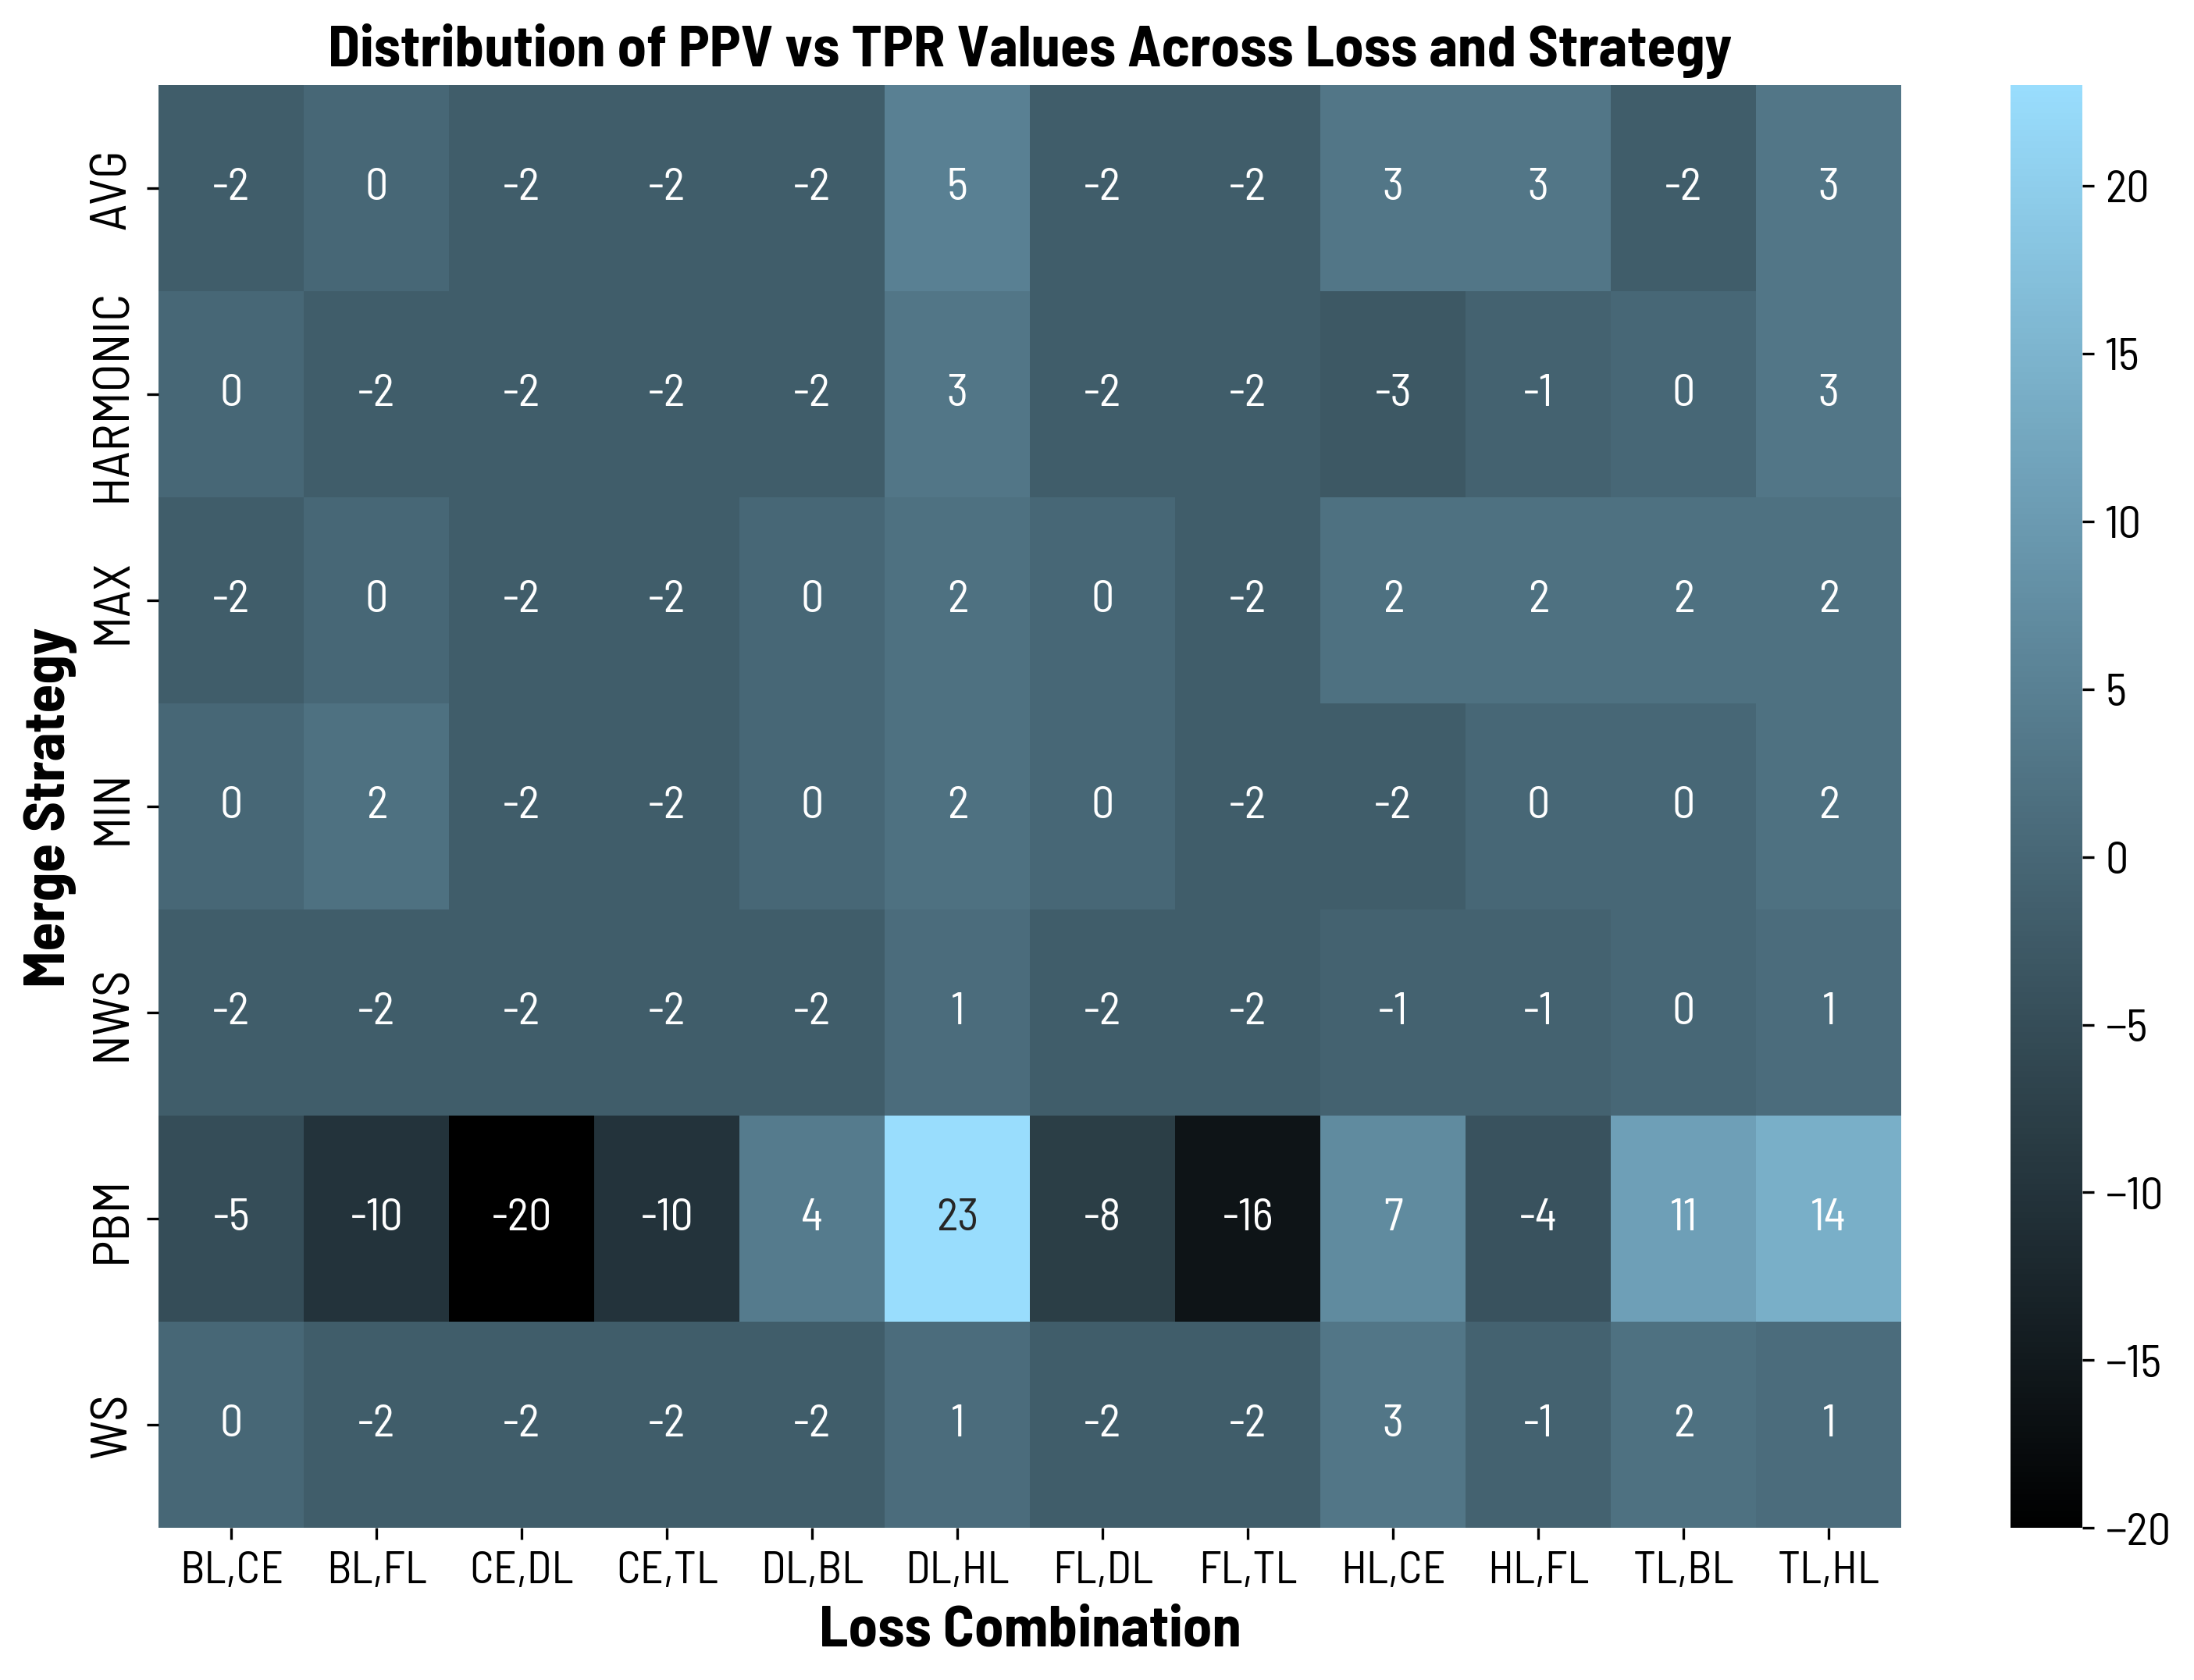
\includegraphics[width=\imgWidthcustom]{images/ppv_tpr_heatmap_double_idrid.png}}
    \subfigure[Distribution of PPV vs. TPR for triple losses]{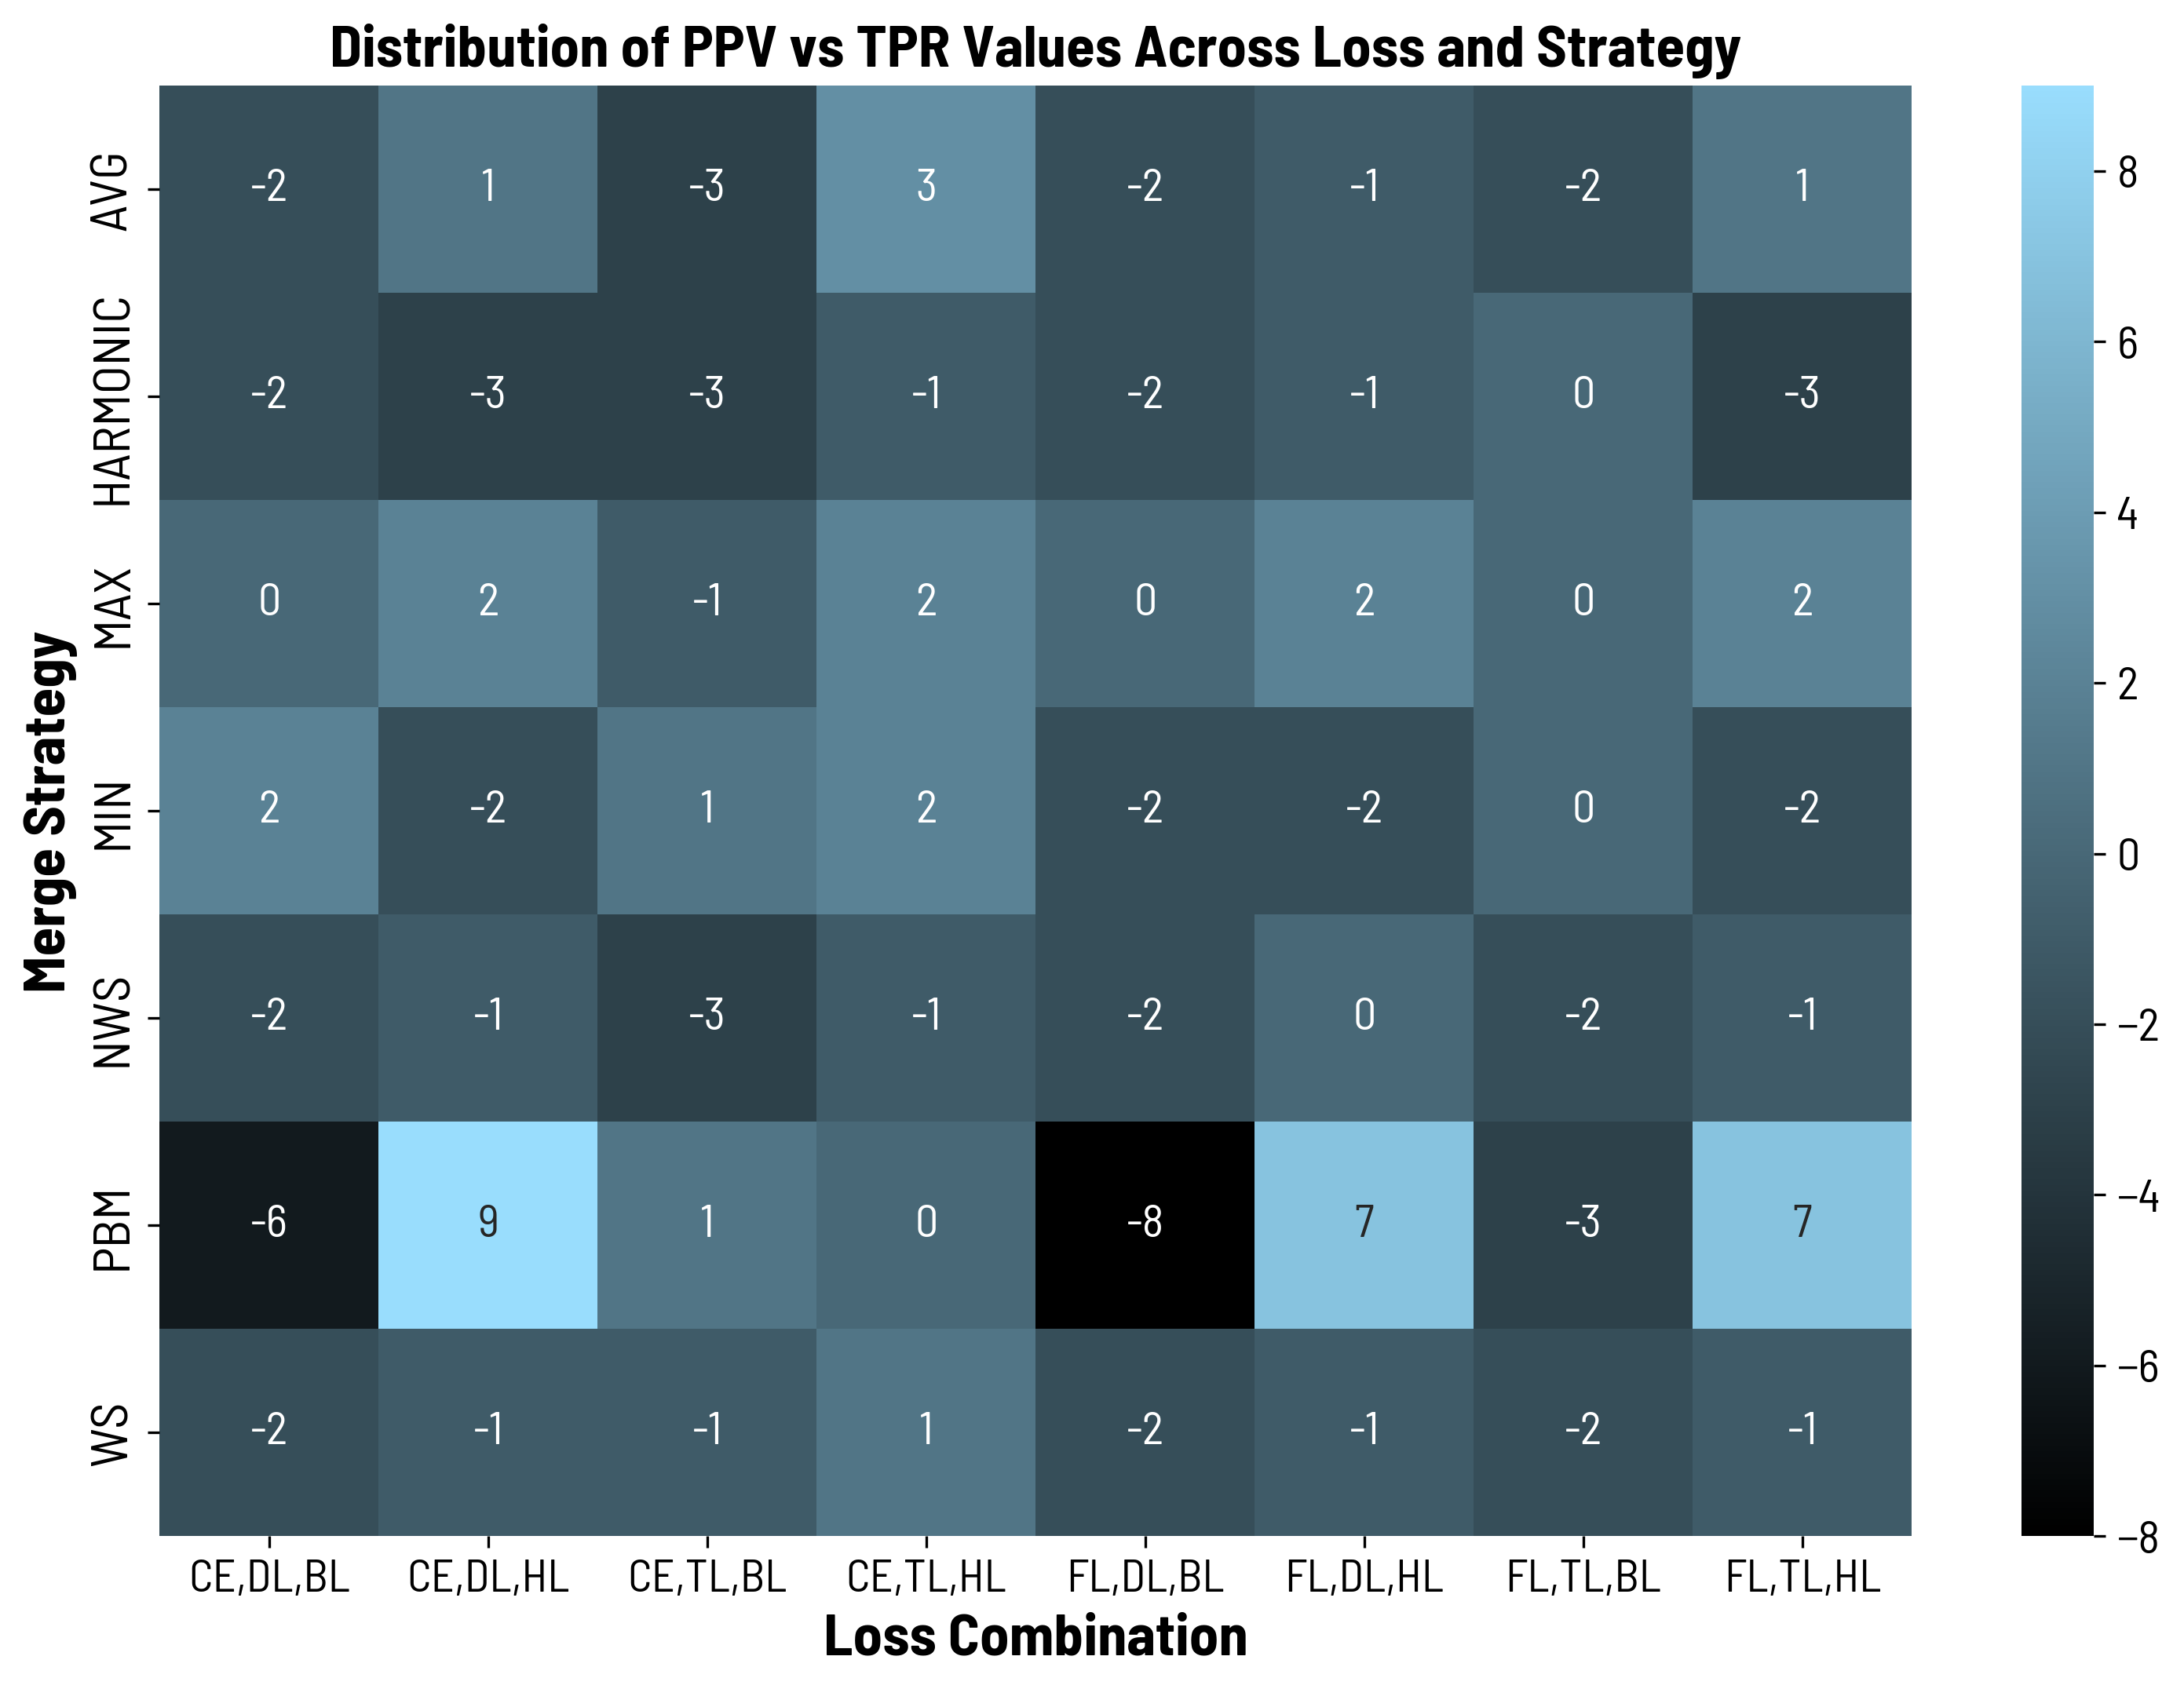
\includegraphics[width=\imgWidthcustom]{images/ppv_tpr_heatmap_triple_idrid.png}}
    \caption[Distribution of PPV vs. TPR Values]{Heatmaps visualizing the relative prevalence as a difference map of PPV and TPR across various loss combinations and merge strategies. Each cell represents a unique combination. Positive values indicate a predominance of TPR, while negative values signify a predominance of PPV.}
    \label{ppv_vs_tpr_idrid}
\end{figure}
\newpage